\documentclass[11pt,Chicago]{uuthesis}
\usepackage{amsfonts,amsthm,mathrsfs}
\usepackage{amsmath,amssymb}
\usepackage[mathscr]{euscript}
\usepackage{thesis}
\usepackage{graphicx}
\usepackage{subfigure}
\usepackage{latexsym}
\usepackage{flafter}
\usepackage{afterpage}
\usepackage{algorithm}
\usepackage{clrscode}
\usepackage{wrapfig}
\usepackage{multirow}
\usepackage{booktabs}
\usepackage{color}
\usepackage[table]{xcolor}
\usepackage{hyperref}
\usepackage{url}


\definecolor{darkgreen}{rgb}{0.0, 0.4, 0.0}
\definecolor{darkblue}{rgb}{0.0, 0.0, 0.6}
\definecolor{darkred}{rgb}{0.6, 0.0, 0.0}

% Make sure subfigures have parentheses around them everywhere
%\renewcommand\thesubfigure{(\alph{subfigure})}
% Make sure subfigures have parentheses around them everywhere
%\renewcommand\thesubfigure{(\alph{subfigure})}

\usepackage{lscape}
%\usepackage{diagram}
%\usepackage{tgrind}
\let \tenrm = \rm 		% This is used in fig*.tex
%\includeonly{}                    % Only front matter and back matter
%\includeonly{chap1}               %  plus chapter 1
%\includeonly{chap2}                %  plus chapter 2
%\includeonly{chap3}                %  plus chapter 3
%\includeonly{appA}                %  plus chapter 3
%\includeonly{chap1,chap2,chap3,chap4}   %  plus all chapters
%\includeonly{chap1,chap2,chap3,chap4,appA}   %  plus all chapters & appendix
%
%\tracingstats=2                % show TeX memory usage
\title{Towards the Theory and Practice of \protect\\ Verifying Visualizations}
\author{Tiago Etiene Queiroz}
\thesistype{dissertation} % or dissertation
\graduatedean{Robert M. Kirby}
\department{Computer Science}
\degree{Doctor of Philosophy}  % of Doctor of Philosophy
\departmentchair{}
\committeechair{Cl\'audio T. Silva}
\firstreader{Robert M. Kirby}
\secondreader{Christopher R. Johnson}
\thirdreader{Luis Gustavo Nonato}
\fourthreader{Juliana Freire}
\chairtitle{Professor}
\submitdate{August 2013}
\copyrightyear{2013}
% Chapter is one level, section and subsection are the next two levels.
\fourlevels
\dedication{To my beloved parents.}
 \inputpicturetrue  % By Jeff McGough. See uuguide and private thesis.sty
%\inputpicturefalse % To NOT produce pictures, uncomment this line


\theoremstyle{plain}
\newtheorem{thm}{Theorem}[section]

\theoremstyle{definition}
\newtheorem{dff}[thm]{Definition}

\DeclareMathAlphabet{\mathpzc}{OT1}{pzc}
                                 {m}{it}
                                 
\newcommand{\deliso}{$\proc{DelIso}$}
\newcommand{\mclewiner}{$\proc{MC33}$}
\newcommand{\vtk}{$\proc{VTKMC}$}
\newcommand{\afront}{$\proc{Afront}$}
\newcommand{\matlab}{$\proc{Matlab}$}
\newcommand{\macet}{$\proc{Macet}$}
\newcommand{\mcsimpleflow}{$\proc{MCFlow}$}
\newcommand{\Matlab}{$\proc{Matlab}$}
\newcommand{\snapmc}{$\proc{SnapMC}$}
\newcommand{\setitemsep}{\setlength{\itemsep}{0pt}}

\newcommand{\gc}{\rowcolor[gray]{.9}}
\newcommand{\s}{~~~~}
\newcommand{\cc}{\cellcolor[gray]{.9}}
\newcommand{\vnv}{V\&V}
\newcommand{\cs}{CS}
\newcommand{\cse}{CS\&E}
\newcommand{\mc}{\textsc{MC33}}
\newcommand{\cmc}{\textsc{C-MC33}}





\begin{document}
%% Comment out items by inserting a percent % character
\frontmatterformat
\titlepage
\copyrightpage
\committeeapproval
%\readingapproval
\preface{abstract}{Abstract}
\dedicationpage
\begin{epigraph}
``No amount of experimentation can ever prove me right; a single experiment can prove me wrong.''
\begin{flushright} -- Albert Einstein \par\end{flushright}
\end{epigraph}
\setcounter{tocdepth}{3}    %How many levels to include in TOC
\addtocontents{toc}{\protect\sloppy}    %Keeps long chapters within page # margins
\tableofcontents
\listoftables
\listoffigures
%
% Optional front page, made from source "notation.tex".
% If you don't need it, then don't use it.
%
%\optionalfront{Notation and Symbols}{\input{notation.tex}}
\preface{acknowledge}{Acknowledgments}
\maintext       % Start normal page numbering. Parts and chapters follow.
\chapter{Geometry of Isosurfaces}\label{chap1}

Bla Bla Bla 

\section{Introduction}
\label{chap1:sec:intro}

In this age of scientific computing, 
the simulation science pipeline of mathematical
modeling, simulation and evaluation is
a rendition of the scientific method as commonly employed as
the traditional experimental pipeline.
Critical to this simulation approach is
the evaluation stage in which numerical
data are post-processed, visualized and 
then examined in order to answer the original
queries that instigated the investigation.
In fact, visualization of scientific results has become
as much a part of the scientific process as 
mathematical modeling or numerical simulation.  
% CITATION NEEDED.

Despite its growing importance in the
scientific computing process, visualization has not fallen under the same
rigorous scrutiny as other components of the pipeline
like mathematical modeling and numerical simulation.
Unlike in traditional computational science and engineering areas,
there is no commonly accepted framework for verifying the accuracy, reliability, 
and robustness of visualization tools. This precludes
a precise quantification of the visualization error budget in the 
larger scientific pipeline.
Furthermore, very few investigations have focused on how the error originating from 
other components of the computational pipeline
impacts visualization algorithms. % CITATION NEEDED

In this work, we advocate the use of techniques from the
\emph{verification and validation} process used in the engineering
community (Section~\ref{chap1:sec:vv} presents V\&V in more detail). While
the lack of a well-established framework for verifying visualization
tools has meant that a variety of analysis techniques have been
developed~\cite{zhou01,tory04}, we believe that visualization 
has achieved sufficient importance to warrant investigation of
stricter verification methodologies. Several authors have
already asserted this need~\cite{globus95,kirby-vv-08}, and in this work we
present techniques that are a concrete step towards reducing the
gap between best practices in simulation science and visualization.


The purpose of this work is to present a verification methodology
for visualization tools that has comparable rigor to that of other 
components of the computational scientific pipeline. More specifically, we set out
to define a verification methodology in the mold of the area of V\&V, 
in the context of visualization.
Furthermore, we illustrate our proposal by testing several publicly 
available isosurface extraction
codes to the verification procedure, giving a detailed 
description of the steps involved in the process.

It is important to emphasize that the point of verification procedures
is not to compare algorithms to one other with
the hope of finding the best alternative.
This procedure equips developers of new algorithms and/or 
implementations with a process that provides a systematic way 
of identifying and correcting errors in both algorithms and implementations.
The goal is to provide users with a methodology that will give them a
more concrete model for the behavior of the implementation, which will
increase confidence in the visualization tools. 
As we will show, a fair verification analysis can 
bring out unforeseen behavior, and quickly detect implementation problems that
might not be caught through standard comparisons or visual inspection.

The contributions of this work are threefold. To the best of our
knowledge, we, for the first time, apply the framework of 
verification to assess the correctness of visualization tools.
Furthermore, we provide a detailed description of how to accomplish the 
verification procedure by subjecting different isosurfacing tools 
to the battery of tests comprising the V\&V process. 
Our second contribution is the underlying mathematical analysis and associated 
manufactured solutions developed to analyze the isosurfacing methods.
We should clarify that when applying MMS for other techniques (even in
the case of isosurface extraction), the theoretical analysis should be
tailored to the particular features of these algorithms.

The manufactured solutions presented here are simple but
general enough to be promptly employed for evaluating other 
visualization tools besides isosurfacing.
Our third contribution is a comprehensive set of results obtained
using the technique, including the finding of implementation errors in
two publicly available isosurface extraction codes.

%
\section{Validation and Verification}
\label{chap1:sec:vv}

In this section we provide a brief introduction to the idea of
\emph{verification and validation} (V\&V), and in particular, its
application in visualization scenarios. We will also review 
efforts to verify implementations in the specific context of
isosurface extraction.
% In the specific context of
% isosurface extraction, we 
% In this section we provide a brief discussion as to what is meant by
% validation and verification (V\&V) in visualization, and also to
% point out what is not meant by V\&V in visualization.  Both are
% equally important issues to clarify.
% As we are proposing a framework to verify isosurface extraction 
% codes, this section also brings an overview of works
% devoted to analyze the behavior and properties of some
% isosurfacing algorithms without worrying though with the
% correctness of the codes.

% \subsection{Validation and Verification within Visualization}

Babu\v{s}ka and Oden define verification as ``the process of determining
if a computational model obtained by discretizing a mathematical model
of a physical event and the code implementing the computational model
can be used to represent the mathematical model of the event with
sufficient accuracy'' \cite{babuska04}.  Although they review the concept 
only in the context of computational science and engineering applications, 
it is important to appreciate that the same idea applies to
scientific visualization. \emph{Verification is about investigating to
what extent a (numerical) approximation scheme -- both in algorithm
and corresponding implementation -- represents the desired mathematical
model}. Validation, on the other hand, is about ensuring that the
model represents physical reality. In this paper, we will concern
ourselves only with verification, under the assumption that the 
model has been validated by the user of the technique. This is the
perspective Kirby and Silva suggest for ``Verifiable Visualization''
\cite{kirby-vv-08}.

% A solid introduction to the concepts of validation and verification 
% as they apply to computational science and engineering was
% provided by Babuska and Oden in \cite{BabuskaO4}. 
% In accordance with Babuska and Oden verification can be defined as

% Although verification is only one component comprising the
% V\&V process (for the complete description of the V\&V process
% see~\cite{BabuskaO4}), it represents the core element as to inspect the
% computational side of the modern scientific experimentation. As visualization mostly
% relies on computational procedures, Kirby and Silva \cite{kirby-vv-08} 
% suggest recently to extend the V\&V idea to what they call ``Verifiable Visualization''.

One of the main requirements for verifiable visualization is to have 
a rigorous analysis which predicts the results of the algorithm and
its implementation when evaluating it on a known model problem.  The
more complete this analysis is, the more thorough the testing procedures
can be. This \emph{continuous process} of verification through refinement
of key controllable input parameters of the method (such as grid spacing) 
and testing is different from a one-shot process.
%
% The purpose of verifiable visualization is not to declare, at the outset, that
% a particular algorithm and implementation has been verified
% in the same way that a drug is declared FDA approved; rather,
%
The verification process should involve a suite of tests with
corresponding results from which one can
progressively increase reliance on the method under analysis. 
When appropriately applied, verification 
provides ways to appreciate the nuances of the applicability of the
method. As we will see in this paper, writing down the analysis for the
expected result of isosurface extraction gives us concrete
bounds on what features we can expect the resulting surface to have,
and these are extremely important for users.

% carlos: This is a really angry paragraph - we'll piss off readers
% this way.
%
% A common practice by the visualization community is to attempt a form of 
% verification through elementary tests towards 
% verifying the basic running of a visualization technique, 
% and then use that visualization technique on 
% ``real-world'' data.  
% What is the value of running on
% realistic data?  Many have convinced themselves that this
% is the means of convincing their intended audience of
% the wide applicability of their methodology.  However,
% from the computational science and engineering perspective, 
% the value of ``real data'' is that it helps to provide
% a scenario in which things can fail -- a scenario 
% that provides insight into how the method performs.
% The challenge, in part, within the visualization community 
% is to devise manufactured test cases which by
% application of a visualization technique provide a
% quantitative means of assessing success or failure 
% (or gradations therein).
%
% carlos: this is the structure 
% People typically use ``real data'' to test techniques. They should
% instead write down a model, expected outcomes, and see if their algos
% satisfy that. As we will show in Section foo, this not only helps pin
% down the characteristics of the technique, but is very effective at
% uncovering subtle bugs in the implementation.

A common practice in the visualization community is to test
implementations by using complicated, ``real-world'' datasets. The
value of these tests is that they provide evidence of the algorithm's applicability. We
advocate a complementary approach: developers should carefully
manufacture test cases that can be mathematically modeled and
analyzed, called \emph{manufactured solutions}. These manufactured
solutions can then be used to test the implementations. In this paper, we present
analysis that describe the expected rate of convergence of several
isosurface features, and test implementations acting on our model problems
using simple analytical volumes. As we show in Sections~\ref{chap1:sec:iea} 
and~\ref{chap1:sec:res}, this method helps pin down the mathematical characteristics 
of the technique, and, more practically, it is quite effective at uncovering 
implementation bugs.

%between simple to ``real'' to 
%be populated with manufactured solutions which by
%application of a visualization technique provide a
%quantitative means of assessing success or failure 
%(or gradations therein).  
% The key is to appreciate that
% all forms of approximation require compromise, and that
% it is imperative to the scientific effort to know
% both the strengths and weaknesses of the methods 
% which we employ.

% Manufactured solutions should not be those solutions
% which help demonstrate the features of a method.  
% These solutions, often generated and
% prominently displaced as the motivation or teaser
% of a method are often numerous and easy to construct.  

The challenge behind manufactured solutions is to construct them in a
way that allows us to predict the expected behavior of the method
under investigation.  Moreover, the manufactured solutions should tax
the method vigorously, bringing out potential problems. In
Section~\ref{chap1:sec:dis}, we will present some situations where
incorrectly chosen manufactured solutions have a big impact in the
results.  We do so to emphasize that all components of the pipeline,
even the construction and evaluation of the manufactured solutions,
must be meticulously handled to maintain the rigor of the verification
process.


%


%
\subsection{Isosurface Extraction Algorithms}
\label{chap1:sec:prevwork}

Isosurface extraction is a popular visualization technique, being a
tool currently used in science, engineering, and applications.
This popularity makes it a natural target for this first application of
verification mechanisms in the context of visualization.
%
This same popularity has also driven a large body of work
comparing different isosurface extraction algorithms.

Previous researchers have examined topological 
issues~\cite{ning93, Lewiner:2003},
mesh quality~\cite{Dietrich:TVCG:2008,Schreiner06},
accuracy~\cite{patera04,zhou01}, and
performance~\cite{Sutton00acase}. The influence of different reconstruction schemes and 
filters in scalar visualization has also been examined~\cite{Hamish06,Pommert02}.
In this paper, we focus on techniques to verify the correctness of
algorithms and their corresponding implementations. In particular, we
provide mathematical tools that other researchers and developers can
use to increase their confidence in the correctness of their own
isosurface extraction codes.  A traditional way to test
implementations in scientific visualization is to perform a visual
inspection of the results of the Marschner-Lobb
dataset~\cite{marschnerlobb}. In the context of isosurface extraction,
researchers routinely use tools such as Metro~\cite{Cignoni:1998:MET} to
quantitatively measure the distance between a single pair of surfaces.
We argue that the methodology presented here is more effective and more
explicit at elucidating a technique's limitations. In particular, our proposal
pays closer attention to the interplay between a theoretical
convergence analysis and the experimental result of a \emph{sequence} of
approximations.

% carlos: we need to cite crj's "visualizing errors" here.. this is an
% error quantification technique.
Globus and Uselton~\cite{globus95} and more recently
Kirby and Silva~\cite{kirby-vv-08} have pointed out the need 
for verifying both visualization techniques and the corresponding
software implementations. In this paper, we provide concrete tools for
the specific case of isosurface extraction. Although this is only one
particular technique in visualization, we expect the general technique
to generalize.

% As can be seen from the discussion above, the visualization literature 
% has lagged behind in
% verifying visualization codes. Some authors argue that this fault is due to the lack
% of a specific methodology, that is, particular verification approaches must be set forth  
% in the context of visualization. The present work aims at presenting a 
% framework to verify isosurfacing tools which follows
% the well established verification methodology usually employed in the
% V\&V field. In fact, we shall show that even simple manufactured solutions
% can reveal unexpected behavior, allowing not only to better understanding
% the conduct of visualization tools but also find out errors in computational codes.

It is important to again stress that verification is a \emph{process}: even
when successfully applied to an algorithm and its implementation, 
one can only concretely claim that the implementation behaves correctly
(in the sense of analyzed predicted behavior) for all test cases to which
it has been applied.  Because the test set, both in terms of model
problems and analyzed properties, is open-ended and ever increasing, 
the verification process must continually be applied to previous and
new algorithms as new test sets become available.  This does not, however,
preclude us from formulating a basic set of metrics against which
isosurface extraction methods should be tested, as this is the starting
point of the process.  This is what we turn to in the next section.

%
\section{Verifying Isosurface Extraction Algorithms}
\label{chap1:sec:iea}

\begin{algorithm}
\begin{codebox}
\Procname{$\proc{MMS}(f, u, h_1)$}
\li \Comment Let $f$ be a scalar field containing the solution surface $S$
\li \Comment Let $u$ be a given property ($f$, normals, area, etc.)
\li \Comment Let $h_1$ be the initial grid size
\li \For $i \gets 1$ \To $n$
\li     \Do $G_{h_i} \gets $ an approximation of $f$ at grid size $h_i$
\li         $S_{h_i} \gets $ an approximation of $S$ computed from $G_{h_i}$
\li         $E_{h_i} \gets || u(S_{h_i}) - u(S)||_u$
\li         $x_i \gets \log h_i$, $y_i \gets \log E_{h_i}$
\li         $h_{i+1} \gets h_i / 2$
        \End
\li $\tilde{q} \gets $ slope of best-fit linear regression of $(x_i, y_i)$
\li Compare $\tilde{q}$ and $q$
\end{codebox}
\caption{\label{alg:manufactured-solutions}Overview of the method of manufactured solutions (MMS).}
\end{algorithm}

In this section, we describe the technique we use for verifying
isosurface extraction algorithms, namely the \emph{method of manufactured
solutions} (MMS). We illustrate a possible implementation of MMS in
Figures~\ref{alg:manufactured-solutions} and~\ref{fig:mms-flow}. This 
technique requires us to write down the expected behavior of particular 
features of interest of the object (or model problem) 
being generated. In our case, we are generating triangular
approximations of smooth isosurfaces, and the features of interest are
geometric surface convergence, convergence of normals, area and
curvature. 

To use MMS, we first accomplish a mathematical analysis of
the expected convergence rate of the features (or characteristics) of interest, 
known in the numerical literature as the \emph{formal order of accuracy} of the
characteristic. This analysis is done for solutions of the problem that can
be conveniently described and analyzed (these are the manufactured
solutions). Then, the code is executed with progressively refined
versions of the data that is used in the generation or sampling of 
the manufactured solution. Finally, the empirical convergence rate is compared to the
one predicted by the analysis.  When the convergence rates are
comparable, we increase our confidence in the algorithm.
%
If the realizable behavior disagrees with the analysis, either (1) the analysis 
does not correspond to the correct behavior of the algorithm, (2) the assumptions
upon which the analysis was build were violated by the input data and hence
the predicted behavior is not valid for the circumstances under investigation, or (3) 
there are issues with the algorithm or with the implementation of the 
algorithm (depending on access to source code
and algorithmic details, one may not be able to distinguish between
these two -- algorithmic or implementation -- and hence we in this work 
always consider them together. Given sufficient information, the
verification process can help further delineate between these
two issues). Notice, however, that all three situations
warrant further investigation. In the following sections, we will discuss
these issues in more detail.  Let us first clarify how
we will arrive at theoretical and empirical convergence rates.

%\subsection{Approximation Error}
For a fixed grid size, we will strive to write the approximation error
between the desired isosurface property and its approximation by:
%% From the analysis presented above we can see that, for a fixed grid size, the approximation error 
%% between the exact isosurface and its approximation is given by:
%If we write $u_k$ as an expansion of Taylor series, we may assume that the truncation term $O(k^p)$ is the one that dominates error, where $p$ is the \emph{theoretical convergence rate}. Thus we can write the discretization error as:

\begin{equation}
E = |u_{approx} - u_{exact}|_u = O(h^p) = \alpha h^p
\label{eq:theoretical-convergence-rate}
\end{equation}
\noindent where $u_{approx},u_{exact}$ are the approximated and 
exact values of a property $u$,  
$|\cdot|_u$ is the norm used to compare the approximate and exact property,
$p$ is the order of accuracy and $\alpha$ is a constant. 
Practically speaking, the polynomial expression
(\ref{eq:theoretical-convergence-rate}) is not very convenient for numerical 
experimentation, as 
it is hard to find the value of $p$ from the direct plot of $h$ against $E$.
The standard technique to estimate $p$ is to linearize by
working on a log-log scale:
\begin{equation}
 \log E = \log (\alpha  h^p) = \log \alpha  + p \log h.
\label{eq:error-log-evaluation}
\end{equation}

Using this linearized version, we estimate $p$ from the slope of 
the line that best fits the points $(\log h,\log E)$ in a
least-squares sense. We use this technique in Section~\ref{chap1:sec:res}
when testing the isosurface codes.

% Why do we use order of accuracy?
MMS critically depends on an analysis of the order of accuracy of
expected solutions. Although this seems quite simple, the order of
accuracy under a sensitive norm like $||\cdot||_\infty$ has shown in
practice to be very effective in bringing out implementation errors in
numerical approximation schemes~\cite{Roy2005,babuska04}. In this
paper, we show that this analysis is just as effective for isosurface
extraction. In addition, we believe the convergence analysis required
by MMS is interesting in its own right. As we will discuss in
Section~\ref{chap1:sec:dis}, it helps to shed light on the consequences of
implementation choices.
%
%% Among the mathematical tools employed to verify
%% numerical codes, order of accuracy analysis plays a special role,
%% providing a very efficient mechanisms to check the correctness and
%% accuracy of numerical approximation
%% schemes~\cite{Roy2005,babuska04}. 
%
%% As it will be discussed later, order
%% of accuracy analysis enables us to better understand the behavior of
%% algorithms as well as to tackle implementation aspects while still
%% being very effective in elucidating coding errors.  Such versatility
%% motivates its use in the verification of isosurface methods, as
%% describe in what is to follow.


%% \subsection{Manufactured Solution}

%% The literature of V\&V has presented different methodologies for
%% verifying numerical codes in the field of engineering and scientific computing,
%% being the \emph{method of manufactured solution} (MMS) one of the most widespread
%% procedure.
%% The reasoning behind MMS is to choose a solution and use it to generate 
%% a set of input data to the computational code under verification, checking
%% whether the output behaves as the original solution. When used with
%% systematic grid refinement, MMS turns out an extremely reliable
%% code verification mechanism.

\begin{figure}
\centering
\includegraphics[width=0.95\linewidth,keepaspectratio=true]{chapter1/figures/mms.pdf}
\label{fig:mms-flow}
\caption{Workflow for the method of manufactured solution (Figure \ref{alg:manufactured-solutions}), clockwise from the top left.}
\end{figure}

%Numerical simulation of partial differential equations is a 
%powerful tool to help scientist to predict and understand several physical behavior.
%In order to build confidence in numerical simulation results, scientists have to 
%verify correctness of the code used to generate those solution. One
%of the traditional methods for code verification is the \emph{method of exact solution}. 
%This method consists in compare the numerical results against the analytical (exact)
%solution of the partial differential equations involved. The main problem with this 
%approach is that the exact solution is often not available or is a solution of
%a simplified model of the equations being solved.
%
%The \emph{method of manufactured solution} (MMS) is an alternative for code verification 
%of computational simulations. The idea is to choose a solution and use it to generate 
%a source term for the original set of equations. Thus, this ``manufactured'' solution is 
%an exact solution for the original set of equation with the correspondingly 
%generated source term.

In the context of isosurface methods, manufactured solutions can be built by
specifying a ``solution surface'' to be the exact solution and deriving a 
scalar field that contains such a solution surface as a level set. The 
verification methodology then proceeds as following: 
(1) use the manufactured scalar field as input for the isosurfacing 
methods, (2) run the methods, and (3) check the output surface against 
the solution surface (sometimes called the {\em ansatz solution} within
the mathematical verification literature).
In many cases, the manufactured scalar field can be derived analytically, 
making the observed order of accuracy tractable (we give
examples in next section).

%% The overall methodology for
%% verifying isosurface tools through manufactured solution can be stated as follows:
%algorithm \ref{alg:manufactured-solutions} presents the overall methodology for verifying
%isosurface tools using the method of manufactured solution. Details
%about how to computed the errors involved in the convergence analysis
%will also be given in next section.
%% In Algorithm~\ref{alg:manufactured-solutions} given above, $\tilde{q}$ and $q$ are the observed and 
%% analytical order of accuracy. Details about the metric $|\cdot|_u$ will be given in next section. 

%% \subsection{Formal order of accuracy}

%% Order of accuracy aims at deriving a mathematical framework
%% towards understanding, from a theoretical point of view, 
%% at which rate the approximations errors generated by isosurfacing schemes converge to the real isosurface 
%% when successive refinement is applied in the background domain.
%% More specifically, we analyze how the approximate vertices, normals, area, and curvatures
%% tend to their exact counterparts when ``finer and finer'' background grids are employed. 

In what follows, we will derive expected orders of accuracy for
several features of surfaces produced by isosurface extraction codes. We keep
our assumptions about the actual algorithms to a minimum to maximize
the applicability of the arguments given. We essentially only assume
that the maximum triangle size can be bounded above at any time, and
use Taylor series arguments (under assumptions of smoothness) 
to derive convergence rates. 
%
It is important to point out that order of accuracy analysis of
polyhedral surfaces has been studied by many
researchers~\cite{meek2000,xu2006,zxuLNCS05,hildebrandt06}.  In
fact, the results presented below are in agreement with the ones
reported in the literature. However, because we are considering
isosurface extraction, some of our arguments benefit by being
able to be condensed to simpler statements.

\subsection{Convergence of Vertex Position}
\label{subchap1:sec:vertex-order-of-accuracy}

We start our analysis of isosurface extraction by studying the
convergence of vertex positions. We analyze this convergence
indirectly by relating the values of the scalar field at the vertex
points and the distance between the vertices and the correct
isosurface. Given a value $\lambda$ such that the exact isosurface $S$
is defined by $f(x,y,z) = f(\vec{v}) = \lambda$, the \emph{algebraic}
distance of $\vec{v}$ to $S$ is defined as $|f(\vec{v}) - \lambda|$
\cite{Taubin94}. Notice that algebraic distances only makes sense
for implicit surfaces: it requires a scalar field. In addition, 
we restrict ourselves to \emph{regular} isosurfaces,
ones where for every point $x$ in $S$, $|\nabla f(x)|$ exists and
is nonzero.
%
Then, the geometric distance between
$\vec{v}$ and $S$ is approximated by $|f(\vec{v}) - \lambda| / |\nabla
f(\vec{v})|$ \cite{Taubin94}. We illustrate this relation
in Figure \ref{fig:algebraic-distance}. Since, by assumption, 
$|\nabla f(x)| > k$ for some
$k > 0$, and all $x$ in $S$, convergence in algebraic distance implies convergence in
geometric distance. Convergence in algebraic distance, however, is much
more tractable mathematically, and this is the item to which we turn our focus.

Many isosurface methods estimate vertex positions through linear
interpolation along edges of a grid.
Let $f:U\subset\mathbb{R}^3 \rightarrow \mathbb{R}$ be the a smooth 
real function defined in a 
subset $U=[a_x,b_x]\times[a_y,b_y]\times[a_z,b_z]$, where $[a_i,b_i], i \in {x,y,z}$ 
are real intervals.
We assume the intervals $[a_i,b_i]$ have the same length and 
let $a_x=x_0,\ldots,x_n=b_x$, $a_y=y_0,\ldots,y_n=b_y$, and
$a_z=z_0,\ldots,z_n=b_z$ be subdivisions for the intervals such that
$x_i = x_0+ih$, $y_i = y_0+ih$, $z_i = z_0+ih,\, i=0,\ldots,n$, 
where $h$ is the grid size and 
$c_{ijk}=[x_i,x_{i+1}]\times[y_j,y_{j+1}]\times[z_k,z_{k+1}]$
is a grid cell. 
\begin{figure}
\centering
\includegraphics[width=.75\linewidth]{chapter1/figures/algebraic.pdf}
\caption{The distance between a point $\vec{v}$ and the isosurface $S$
  with isovalue $\lambda$ can be approximated by the algebraic
  distance divided by the gradient magnitude of the scalar field at $\vec{v}$,
  $|f(\vec{v})-\lambda| / |\nabla f(\vec{v})|$. In the figure, the
  thick circle represents the isosurface $S$ and the fainter isolines
  illustrate changes in gradient magnitude: in regions of small
  gradient magnitude, the algebraic distance is small but geometric
  distance is large, and vice-versa for large gradient magnitude.}
\label{fig:algebraic-distance}
\end{figure}
Through a Taylor series expansion of $f$, one can evaluate $f$ 
at a point $\vec{p}\in c_{ijk}$ as:
\begin{equation}
f(\vec{p}) = f_{ijk} + \nabla f_{ijk}\cdot \vec{\delta} + \frac{1}{2}\vec{\delta}^T H(\vec{\xi}) \vec{\delta}
\label{eq:taylor}
\end{equation}
\noindent where $f_{ijk}=f(x_i,y_j,z_k)$, $\nabla f_{ijk}$ is the gradient 
of $f$ in $(x_i,y_j,z_k)$,
$H(\vec{\xi})$ is the Hessian of $f$ at a point $\vec{\xi}$ 
connecting $(x_i,y_j,z_k)$ and $\vec{p}$, 
and $\vec{\delta} = (u,v,w)^T$ is such that $\vec{p} = (x_i+uh,y_j+vh,z_k+wh)^T$.

Let the linear approximation of $f$ in $\vec{p}$ be defined by
\begin{equation}
\tilde{f}(\vec{p}) = f_{ijk} + \nabla f_{ijk}\cdot \vec{\delta}
\label{eq:linear}
\end{equation}
\noindent and consider a point $\vec{x_\lambda}$  such that $\tilde{f}(\vec{x_\lambda}) = \lambda$, that is,  
$\vec{x_\lambda}$ is a point on the isosurface $\lambda$ of $\tilde{f}$.

The algebraic distance between the exact isosurface $f(x,y,z) = \lambda$ and
the linearly approximated isosurface can be measured by 
$|f(\vec{x_\lambda}) - \lambda|$. From Equations~\ref{eq:taylor} and~\ref{eq:linear} one can 
see that
\begin{equation}
\begin{array}{c}
\displaystyle{|f(\vec{x_\lambda}) - \lambda| = |f_{ijk} + \nabla f_{ijk}\cdot \vec{\delta} + \frac{1}{2}\vec{\delta}^T H(\vec{\xi}) \vec{\delta} -\lambda| =}\\
|\tilde{f}(\vec{x_\lambda}) + O(h^2) -\lambda| = O(h^2)
\end{array}
\label{eq:algebraicerror}
\end{equation}
\noindent thus, the linearly approximated isosurface is of second-order accuracy.

%% Algebraic error has been adopted as one of the verification mechanisms presented in next section. We have opted
%% by algebraic error rather than geometrical error because the former is as much effective as geometrical 
%% error in the context of verification while still being computationally less expensive to compute.

%\noindent the approximation error can be written as:
%\begin{equation}
%|f(\vec{p}) - \tilde{f}(\vec{p})| = |\frac{1}{2}\vec{\delta}^T H(\vec{\xi}) \vec{\delta}| = O(h^2).
%\label{eq:linearerror}
%\end{equation}

%As isosurfacing methods place the vertices of the approximate isosurface on a level set of $\tilde{f}$, 
%these approximate vertices
%should converge to the real isosurface at the same rate as $\tilde{f}$ converges to $f$.
%In the case of linear interpolation, the rate of 
%convergence is quadratic, as one can be seen from Equation (\ref{eq:linearerror}).

\subsection{Convergence of Normals}
\label{chap1:sec:normalconvergence}

Assume, generally, that the scalar field $f(x,y,z)=\lambda$ can be
locally written as a graph of a function in two-variables
$g(x(u,v),y(u,v))=\lambda-f(x(u,v),y(u,v),z_k)$, as illustrated in
Figure~\ref{fig:graphfunct}, where $x(u,v) = x_i+uh$ and
$y(u,v)=y_j+vh$. This is acceptable because we have already assumed
the isosurface to be regular. Still without losing generality we
write $g(x(0,0),y(0,0)) = 0$, that is, the isosurface
contains the point $(x_i,y_j,z_k)$. Let  
$\vec{\Phi}(u,v) = (x(u,v),y(u,v),g(x(u,v),y(u,v)))$ be a parametrization 
for the isosurface $f(x,y,z)=\lambda$ in $c_{ijk}$ and
% \begin{equation}
% \frac{\partial\vec{\Phi}}{\partial u}\times\frac{\partial\vec{\Phi}}{\partial v} = 
% h^2\left(\begin{array}{c}
%              -\frac{\partial g}{\partial x}\\
% 	     -\frac{\partial g}{\partial y}\\ 
% 	     1\end{array}\right) = h^2 \vec{n_0}
% \label{eq:normal_exact}
% \myspacemini
% \end{equation}
\begin{equation}
\frac{\partial\vec{\Phi}}{\partial u}\times\frac{\partial\vec{\Phi}}{\partial v} = 
h^2\left(-\frac{\partial g}{\partial x},\\
	     -\frac{\partial g}{\partial y},\\ 
	     1\right)^T = h^2 \vec{n_0}
\label{eq:normal_exact}
\end{equation}
\noindent be the normal vector in $\vec{\Phi}(0,0)=(x_i,y_j,g(x_i,y_j))$ 
(the partial derivatives of $g$ are evaluated at $(x(0,0),y(0,0))=(x_i,y_j)$).

\begin{figure}
  \centering
  \includegraphics[width=0.60\linewidth,keepaspectratio=true]{chapter1/figures/gridcell.pdf}
  \caption{Isosurface local parametrization and approximation.}
  \label{fig:graphfunct}
\end{figure}

Consider now the triangle defined by the points $\vec{p_1},\vec{p_2}$, and $\vec{p_3}$ 
approximating the isosurface
$f(x,y,z)=\lambda$ in the grid cell $c_{ijk}$ (see Figure~\ref{fig:graphfunct}).
Let $\vec{p_1}$ be the grid point $(x_i,y_j,z_k)$, so $\vec{p_1}=\vec{\Phi}(0,0),\, \vec{p_2}=\vec{\Phi}(u_2,v_2)$, and $\vec{p_3} = \vec{\Phi}(u_3,v_3)$. 
Using the cross product in $\mathbb{R}^3$, 
the normal of the triangle $p_1p_2p_3$ can be computed by:
\begin{equation}
\begin{array}{c}
\displaystyle{\vec{n_{p_1p_2p_3}}\!\! =\!\! (\vec{p_2} - \vec{p_1})\times(\vec{p_3} - \vec{p_1})\!\! =} \\
\displaystyle{\left(\!\!\!\!\!\begin{array}{c}
h(v_2g(x(u_3,v_3),y(u_3,v_3)) - v_3g(x(u_2,v_2),y(u_2,v_2)))\\
h(u_3g(x(u_2,v_2),y(u_2,v_2)) - u_2g(x(u_3,v_3),y(u_3,v_3)))\\
%h(u_3g(u_2,v_2) - u_2g(u_3,v_3))\\
h^2(u_2v_3-u_3v_2))
\end{array}\!\!\!\!\!\right).}
\end{array}
\label{eq:normal_tri1}
\end{equation}

Expanding $g(x(u_i,v_i),y(u_i,v_i)),\, i \in \{2,3\}$ in a Taylor
series, some terms cancel and the normal $\vec{n_{p_1p_2p_3}}$ becomes:
% \begin{equation}
% \vec{n_{p_1p_2p_3}} = rh^2
% \left(\begin{array}{c}
% -\frac{\partial g}{\partial x} + O(h)\\
% -\frac{\partial g}{\partial y} + O(h)\\ 
%  1\end{array}\right)
% \label{eq:normal_tri2}
% \myspacemini
% \end{equation}
\begin{equation}
\vec{n_{p_1p_2p_3}} = rh^2
\left(
-\frac{\partial g}{\partial x} + O(h),\\
-\frac{\partial g}{\partial y} + O(h),\\ 
 1\right)^T
\label{eq:normal_tri2}
\end{equation}
where $r = u_2v_3-u_3v_2$. 
Comparing the exact normal vector $\vec{n_0}$ in Equation~\ref{eq:normal_exact} with
$\vec{n_{p_1p_2p_3}}$ above, we recover first-order of accuracy for normals. 
In addition, notice that the usual scheme of estimating vertex 
normals by the arithmetic mean of triangle normals
does not decrease the order of accuracy; that is, vertex 
normals (computed by arithmetic mean) are at least first-order accurate.

\subsection{Convergence of Area}
\label{chap1:sec:areaconvergence}

\begin{figure}
\centering
\includegraphics[width=.8\linewidth]{chapter1/figures/sequence.pdf}
\caption{Uniform convergence does not imply convergence in area. The
  sequence of curves converges uniformly to a straight line, but the
  length of the curves does not change.}
\label{fig:uniformconvergence}
\end{figure}

Currently, much less is known about convergence in area, compared to
convergence of vertices or normals. To illustrate the difficulty
involved in approximating lengths and areas, consider the sequence
of approximations to a straight line shown in Figure \ref{fig:uniformconvergence}. 
Even though the function sequence converges uniformly to the line, 
the length of the approximation stays constant.

To the best of our knowledge, the only relevant results establish
convergence in area given convergence in vertex positions \emph{and}
convergence in normals, such as in Hildebrandt {\em et al.}
\cite{hildebrandt06}. However, the authors only establish
asymptotic convergence, with no order of accuracy associated with
it. The argument is more mathematically involved than space allows
here, so we refer the reader to that paper. Currently, this means that
the only information the observed order of accuracy provides to us is that
if we expect convergence in normals, we should also expect convergence
in area, and vice-versa.

% We assume once again that the isosurface $f(x,y,z)=\lambda$ can be written as
% the graph of a function $g(x(u,v),y(u,v))$ in $c_{ijk}$.

% %, one can compute the area of the isosurface in $c_{ijk}$ as follows:
% %\begin{equation}
% %\int\!\!\!\!\!\int_T \|\vec{n}\| dudv
% %\label{eq:area1}
% %\end{equation}
% %where $\vec{n}$ is the surface normal.
% The approximation error $E_a$ between the area of the exact surface 
% and the area of the triangle (as in Figure~\ref{fig:graphfunct})
% can be estimated using the traditional formula for the area of a parametric surface \cite{Courant},
% as follows: 
% \begin{equation}
% E_a = \left|\int\!\!\!\!\!\int_T \|\vec{n_{p_1p_2p_3}}\|- \|\vec{n}\| \;du\;dv\;\right|
% \label{eq:area1}
% \end{equation}
% \noindent where $T$ is the triangle defining the domain of $\vec{\Phi}$, $\vec{n_{p_1p_2p_3}}$ is 
% the normal of the triangle approximating the surface, and $\vec{n}$ is the normal 
% of the exact surface.

% Using (\ref{eq:normal_tri2}) and Taylor expansion for $\|\vec{n}\|$,
% together with the inequality $|a - b| \le |a| + |b|$, one can write:
% \begin{equation}
% E_a \le \left| \displaystyle{\int\!\!\!\!\!\int_T h^2(r\|\vec{n_0} + O(h)\| + \|\vec{n_0}\|+O(h)) \;du\;dv\;}\right| = O(h^2) \\
% \label{eq:area2}
% \end{equation}

% Therefore, from Equation (\ref{eq:area2}) one can see that the area of 
% the approximated surface has second order of accuracy.

\subsection{Convergence of Curvature}
\label{chap1:sec:curvconvergence}
The following formula gives an estimate of the curvature at a
vertex $p$:
\begin{equation}
K(p) = \frac{2\pi-\sum \theta_{i\,i+1}}{\frac{1}{3}A_{i\,i+1}}
\label{eq:curvat}
\end{equation}
\noindent where $\theta_{i\,i+1}$ and $A_{i\,i+1}$ are the angle 
$\angle p_ipp_{i+1}$ and area of the
triangle $p_ipp_{i+1}$ respectively (summation is over all triangles comprising 
the star of $p$)~\cite{meek2000}. 
Meek and Walton~\cite{meek2000} showed that the curvature computed via 
Equation~\ref{eq:curvat}
does not converge in general; that is, if the vertices of the star of $p$ 
are arbitrarily distributed
around $p$, one cannot expect curvature convergence. In fact, they
described a more general result stating that $O(h)$ accuracy can only be
obtained if the normals are known to have accuracy $O(h^2)$. Subsequently,
Xu~\cite{xu2006} presented a very particular distribution of vertices around $p$
under which the curvature estimated by Equation~\ref{eq:curvat} has accuracy $O(h^2)$. 

Curvature discretization schemes other than the one given in
Equation~\ref{eq:curvat} such as the quadratic-fit and spherical-image method
(see Meek and Walton~\cite{meek2000} for details) also demand
particular vertex distributions to ensure convergence. In our context
of keeping the analysis applicable for many isosurfacing algorithms,
this means we cannot use the lack of observed curvature convergence as an
indication of problematic behavior. Based on the results
mentioned above, one should actually expect curvature not to converge for most
isosurface extraction algorithms. More generally, this indicates a weakness of
MMS, namely that some features of interest (such as curvature)
will not have sufficient theoretical order of accuracy to be used in numerical
measurements. Notice, in addition, that if we had not written down the
theoretical model for curvature convergence, we might have expected
some sort of curvature approximation. Even a negative result such as
the one presented in this section can increase the confidence in the
results generated by an implementation.

% The convergence analysis of triangulated isosurfacing 
% can be accomplished by analyzing how quickly
% the triangular meshes converge to the original isosurface  
% when the background regular grid that supports the isosurface algorithm is 
% successively refined. Mathematically, 
% let $E_{S\tilde{S}_i}$ and $E_{S\tilde{S}_{i+1}}$ be the approximation errors of a given property
% $A:\mathbb{R}^3\rightarrow \mathbb{R}^d$ defined over $S$ and $\tilde{S}$
% in two consecutive grids with spacing $h_i$ and $h_{i+1}$ respectively, where 
% $h_{i+1} = \frac{h_i}{2}$. By conjecturing that the approximation error in two consecutive grids
% are related by:
% \begin{equation}
% E_{S\tilde{S}_{i+1}} = h^\alpha\, E_{S\tilde{S}_i}
% \label{eq:error-relation}
% \end{equation}
% \noindent where $h=h_1$ is the initial grid size, we define the convergence rate 
% (or error order) of the method as the exponent $\alpha$ in equation (\ref{eq:error-relation}).
% A typical approach to compute the convergence rate numerically is 
% to estimate $\alpha$ as the slope of the straight line
% that best fits the points $(\log h_i,\log E_{S\tilde{S}_i}),\; i=1\ldots s$, where $s$
% is the number of grids employed in the experiments.


%
\section{Experimental Results}
\label{chap1:sec:res}

%\subsection{Isosurface Extraction Algorithms Under Verification}
%\label{subchap1:sec:iea}

In this section we present the results of applying the afore-described 
methodology. We use the framework to verify six different isosurface 
extraction codes, namely: VTK Marching Cubes~\cite{lor87},
SnapMC~\cite{Raman:2008:QIM}, Macet~\cite{Dietrich:TVCG:2008},
Dual Contouring~\cite{Ju02}, Afront~\cite{Schreiner06},
and DelIso \cite{Dey07}. All these
implementations are open source and/or publicly 
available\footnote{Links at http://www.sci.utah.edu/\textasciitilde etiene/}.
Before presenting the actual results of subjecting these
implementations to the verification process,
we briefly review their salient features.

%We have chosen such algorithms due to their popularity and similar characteristics, as all of them deal with 
%triangular meshes to approximate the desired isosurface and they also demand a background grid to support the approximation scheme.

%% \subsection{Isosurface Extraction Codes under Verification}

\paragraph*{VTK Marching Cubes:} Marching Cubes~\cite{lor87} (MC) is
arguably the most popular isosurface extraction algorithm.
% THIS SENTENCE SHOULD FIT BETTER SOMEWHERE ELSE IN MOTIVATION 
%and its VTK implementation~\cite{vtk} is widely employed in engineering applications and in life sciences field. 
It reduces the problem of generating an isosurface triangulation
to a finite set of cases by considering the \emph{signs} of 
how the isosurface intersects each cell of a regular background grid.
As there are only 256 different
types of intersections between the isosurface and a regular Cartesian 3D cell, 
a template of triangles is set to each case, making the implementation quite simple 
through a look-up table. The vertices of the triangles lie on 
the edges of the cubic cells, and they are computed by linearly interpolating 
the implicit function values stored at the corners of the grid cell. 

\paragraph*{SnapMC:} SnapMC~\cite{Raman:2008:QIM} is a recently proposed algorithm
that extends the original Marching Cubes look-up table to cases where
the isosurface goes exactly through the corners of the background
grid.  The new look-up table is automatically built by an adaptation of
the convex hull scheme proposed by
Bhaniramka {\em et al.}~\cite{bhaniramka04}. Even though the traditional Marching
Cubes algorithm can easily handle these cases by some kind of symbolic
perturbation, SnapMC \emph{perturbs the scalar field} to avoid edge
intersections close to grid corners. In particular, it changes
the values on the grid so that the surface is ``snapped'' to the grid
corners.

\paragraph*{Macet:} Macet~\cite{Dietrich:TVCG:2008} is another variant of Marching
Cubes that tries to improve the shape of the triangles in a
mesh. Unlike SnapMC, it \emph{perturbs the active edges} of Marching Cubes
cases by moving the vertices before the triangulation step.  The
motivation behind Macet is that poorly-shaped triangles tend to be
generated when the intersection between the isosurface and a grid cell
is approximately parallel to an edge of the grid cell. Therefore, some
corners of the background grid are displaced so as to avoid the
parallel-like intersections.

\paragraph*{Dual Contouring:} Dual Contouring~\cite{Ju02} is a feature-preserving
isosurfacing method to extract crack-free surfaces from both uniform
and adaptive octree grids. This technique can be seen as a combination of
Extended Marching Cubes~\cite{kobbelt01} and SurfaceNets~\cite{gibson98} 
as it makes use of Hermite data and quadratic error function minimization 
to position the vertices of the surface mesh (as Extended Marching Cubes) 
and the dual topology to connect such vertices (as SurfaceNets).  Dual 
Contouring tends to generate better quality triangles than Marching Cubes 
while still being very effective in representing sharp features, rendering this
implicit polygonalization method a good alternative to the popular Marching Cubes.

\paragraph*{Afront:} Afront~\cite{Schreiner06} is an advancing-front method
for surface extraction. Although we focus on applying Afront to
isosurface extraction, it can also be used for remeshing and
triangulating point-set surfaces. The outstanding feature of Afront is
that it generates triangles adapted to the local details of a surface,
namely its maximum absolute curvature. In this sense, Afront is
fundamentally different from the other algorithms we analyze. In lieu
of grid refinement, we will use its $\rho$ parameter to control
triangulation size. Because the manufactured solution we use is a
sphere, reducing $\rho$ by half is roughly equivalent to reducing the
maximum triangle size by half. A full analysis of Afront (and, in
particular, the influence of the other main parameter $\eta$) warrants
further investigation, but is beyond the scope of this paper.

\paragraph*{DelIso:} DelIso \cite{Dey07} is a Delaunay-based 
approach for isosurfacing. It computes the restricted Delaunay triangulation 
from a 3D Voronoi Diagram. We run our tests on a customized version of DelIso 16 bit, 
and our examples use the default set of parameter.

%% Afront provides both surface meshing or remeshing and works at a local or global level.
%% %It was motivated by the fact that classical approaches as marching methods requires 
%% Afront uses two user-defined parameters, namely $\rho$ and $\eta$, to control approximation accuracy and triangle 
%% adaptiveness respectively. The main idea is to use the parameters $\rho$ and $\eta$ to build a guidance field from the input surface whith
%% dictates triangles sizes. 
%% The guidance field gives also an Hausdorff error bound between the original surface and the generated mesh.

In what follows, we present the results of applying the verification process 
to these algorithms. We will describe the manufactured solutions we use and
their observed convergence rate on the isosurface extraction algorithm.

% THIS IS CONTRIBUITION. SHOULD BE MOVED
%A side effect of our experiments is a natural and detailed comparison among such techniques, what can be seen as another
%relevant contribution of this work. 

%As already mentioned, we shall show that well established verification tools also turn out very effective in the context of visualization.
%In fact, we have reached quite surprising and unexpected results by employing a conventional convergence analysis to verify isosurface algorithms.

\subsection{Observed order of accuracy}
\label{chap1:sec:verification-results}

We start by investigating the behavior of the algorithms 
under the manufactured solution given by the
scalar field $f(x,y,z) = x^2+y^2+z^2 - 1$ and isosurface $f(x,y,z) =
0$ in the domain $D=[-4,\, 4]^3$.
%% In this section we presents the scenario where the tests will be performed. The errors formulas are given and the convergence curves as well.
%% Let $f:\mathbb{R}^3\rightarrow \mathbb{R}$ be a smooth function and
%% $S$ the isosurface $f(x,y,z) = \lambda$. 
%% In the following sections, we assume the simple case $f(x,y,z) = x^2 + y^2 + z^2 - 1$ within domain
%% $D=[-4,\, 4]^3$.
Let $\tilde{S}_k$ be a simplicial complex that approximates $S$ for a given 
discretization parameter $k$ (cell size $h$ for marching cubes-based methods, 
accuracy $\rho$ for Afront and maximum edge size $\iota$ for DelIso).

The order of accuracy for VTK Marching Cubes, SnapMC, Macet and Dual
Contouring depends on the cell size $h$. We run our tests with grid
refinement $h_{i+1} = h_{i} / 2$ and initial condition $h_1$. For
Afront, the order of accuracy depends on parameter $\rho$ thus the
refinement is given by $\rho_{i+1} = \rho_{i} / 2$ with initial
condition $\rho_1$. Our customized version of DelIso has an additional parameter $\iota$
that controls the largest edge on the output mesh. In this case, the refinement 
formula is
$\iota_{i+1} = \iota_{i} / 2$.
In the particular case of SnapMC, we set the snap
parameter  $\gamma$ to its maximum value ($\gamma = 1/2$). Even though
the manufactured solution we selected is about as simple as can be
imagined, comparing the formal order of accuracy with the observed one
was enough to suggest bugs in two implementations. The observed
order of accuracy of the examined properties 
is presented on Table~\ref{tab:results}.

\begin{table}
\centering
\begin{tabular}{lrrrr}
\hline
 & Vertex  & Normal & Area & Curvature \\
 & $O(h^2)$ & $O(h)$ & --  & $O(1)$ \\
\hline
VTK MC          &  $1.94$    & $0.93$  & $2.00$      & $-3.35$ \\
SnapMC          &  $1.93$    & $0.82$   & $2.14$     & $-0.29$ \\
Afront$^*$          &  $-0.06$ & $0.80$   & $1.93$     & $-0.27$ \\
%Afront $(h)$    &  $-0.14^*$ & $0.01^*$ & $0.05^*$   & $0.07 $ \\
 Macet$^{1,*}$      &  $0.98$    & $-0.12$  & $0.29$     & $-2.41$ \\
 Macet$^{2,*}$      &  $0.03$  & $0.75$   & $2.02$     & $-0.61$ \\
 DC$^1$         &  $1.02$    & $-0.11$  & $0.69$     & $-2.08$ \\
 DC$^2$         &  $1.96$    & $0.96$   & $1.89$     & $-0.15$ \\
 DellIso      &  $1.49$    & $1.07$  & $2.04$      & $0.07$ \\
\hline
\end{tabular}
\caption{Comparison between formal order of accuracy and observed
  order of accuracy using $f(x,y,z) = x^2 + y^2 + z^2 -1$ as a manufactured solution 
  and for different algorithms. $^1$ indicates the original source 
    code and $^2$ our fixed version.
   $^*$ indicates that a high-order spline was used instead of a 
linear interpolation (Section \ref{chap1:sec:iea}).}
\label{tab:results}
\end{table}

%% As we will discuss,
%% the spherical solution was not taxing enough on some of the codes we
%% used, leadin
%% We were able to find bugs in the some of the codes using $f$ as a manufactured solution. However, due to its simplicity, $f$ is not suitable to evaluate some of the implementations. A detailed discussion is given in the next section.


\begin{figure}
\centering
\subfigure{
\label{fig:meshconver}
\includegraphics[width=0.40\linewidth,keepaspectratio=true]{chapter1/figures/all_meshconv-bug.pdf}}
\subfigure{
\label{fig:normconver}
\includegraphics[width=0.40\linewidth,keepaspectratio=true]{chapter1/figures/all_normalconv-bug.pdf}}
\subfigure{
\label{fig:areaconv}
\includegraphics[width=0.40\linewidth,keepaspectratio=true]{chapter1/figures/all_areaconv-bug.pdf}}
\subfigure{
\label{fig:curvatureconv}
\includegraphics[width=0.40\linewidth,keepaspectratio=true]{chapter1/figures/all_curvconv-bug.pdf}}
\caption{Observed order of accuracy. The implementations of 
Macet and Dual Contouring have a bug that causes the deviation on errors. The black 
continuous line represents the expected behavior. $p$ is the slope of the linear 
regression for each curve.}
\end{figure}


\subsubsection{Algebraic distance}
%\label{subchap1:sec:mesh}

Section \ref{subchap1:sec:vertex-order-of-accuracy} shows that one expects second-order 
convergence for function value on vertices if linear interpolation is used. 
We define the following approximation error on $L_\infty$ norm:
\begin{equation}
E_{k} = \max_{j=1\cdots n}|\lambda - f(v_{j})|
\label{eq:surferror}
\end{equation}
where $\lambda$ is the isovalue of interest, $v_j$ is a vertex of $\tilde{S}$ and 
$n$ the number of vertices. Figure~\ref{fig:meshconver} shows the vertex observed 
order of accuracy.
VTK Marching Cubes, SnapMC have nearly quadratic convergence rates 
as shown in Figure~\ref{fig:meshconver}. Afront shows a zero-order of accuracy 
though it presents very low error (in fact, the lowest in Figure \ref{fig:meshconver}). 
This is due to the Catmull-Rom spline that is being used for surface 
approximation on the voxelized grid. Since it has cubic-order of accuracy, 
even for large values of $\rho$  it can approximate with high precision 
the manufactured solution $f$. Next section shows that this is due to a poor 
choice for a manufactured solution. DelIso implementation has non-zero order 
of accuracy due to an outlier. Large values of $\iota$ causes bad approximations 
of the manufactured solution.
%All other approximation have zero-th accuracy order. 
%A possible explanation for this is that 
%the convergence of algebraic function on vertices does not depend on $\iota$ but on other variable, voxel size $h$.
%Because DelIso uses trilinear interpolation to approximate a surface vertex, the error on vertices remain constant if
%the grid size does not change.


The Macet and Dual Contouring curves suggest that the algorithms converge to 
a fixed value. 
%There are three possible interpretations for this behavior: 
%a) the tests were not correct;
%b) there is another error source (not present or erroneously ignored 
%in the theoretical analysis) that becomes dominant during refinement;
%c) there is a bug in the source code. 
In fact, there was indeed a problem in the implementation
that was affecting the convergence of Macet and Dual Contouring
(specifically, we found a hard-coded limit in the number of steps in a
root-finding procedure that was being triggered by the high resolution
of the volume). Once fixed, we obtain the results shown in Figure
\ref{fig:meshconver-fixed}. Macet and Afront now have similar behavior 
in the observed order of accuracy of vertex position 
(Figure \ref{fig:meshconver-fixed}). This is because both methods use 
high-order interpolation with splines, not linear interpolation as 
assumed before (see Section \ref{chap1:sec:mms-complexity}).

% In order to verify whether the isosurfacing algorithms behave 
% as expected in terms of mesh convergence, we computed the
% error (\ref{eq:surferror}) between the triangular mesh and a sphere 

\subsubsection{Normals}
\label{subchap1:sec:normal-convergence}

Section \ref{chap1:sec:normalconvergence} shows that 
one expects first-order of accuracy for normal computations. 
We define the following approximation error using $L_\infty$ norm:
\begin{equation}
E_{k} = \max_{j=1\cdots n}|\theta_{\sigma_j}|
\label{eq:normerror}
\end{equation}
where $\theta_{\sigma_j}$ is the angle between the normal of 
the triangle $\sigma_j$ and the normal of 
the point in $S$ closest to the centroid of $\sigma_j$.
As shown in Figure \ref{fig:normconver}, VTK Marching Cubes, Afront,
SnapMC and DelIso have good observed order of accuracy above $0.8$. However, only 
VTK Marching Cubes and DelIso present close proximity to linear. 
Macet and Dual Contouring once again do not present a consistent order. 
Figure \ref{fig:normconver-fixed} shows the results after fixing both codes.

\subsubsection{Area}
\label{chap1:sec:area-observed-order-of-accuracy}

Although there is no formal order of accuracy for area, one expects \emph{some}
convergence for it (Section \ref{chap1:sec:areaconvergence}).
We define the following approximation error:
\begin{equation}
E_{k} = |A(S) - A(\tilde{S}_k)|
\label{eq:surfareaerror}
\end{equation}
where $A$ is the area function of a continuous or piecewise-linear surface. 
The results are shown in Figure~\ref{fig:areaconv}. 
VTK Marching Cubes, Afront and DelIso present second-order of accuracy as shown 
in Figure \ref{fig:areaconv}. SnapMC accuracy is slightly better than quadratic due 
to poor approximation for large $h$. The error dropped faster than quadratic when the 
grid was refined for the first time. Macet and Dual Contouring exhibit once again  
unexpected behavior. Unlike the previous time, the curves now seem to diverge 
when $h$ is too small. Once the bug is fixed the convergence curves changes,
and they become quadratic (Figure \ref{fig:areaconv-fixed}).
 
\subsubsection{Curvature}

Section \ref{chap1:sec:curvconvergence} shows that one expects zero-th order of accuracy for 
curvature computation. 
We define the approximation error using $L_\infty$ norm:
\begin{equation}
E_{k} = \max_{j=1\cdots n}|K(v_j) - \tilde{K}(v_j)|
\label{eq:curverror}
\end{equation}
where $K(v)$ is the Gaussian curvature at $v \in S$ and $\tilde{K}(v)$ is the Gaussian curvature at $v \in \tilde{S}$. In this
particular case where $S$ is a sphere, $K(v) = 1$ for every $v \in S$. The results 
are shown in Figure~\ref{fig:curvatureconv}.
DelIso, Afront and SnapMC are close to zeroth-order accuracy. The
curvature order of accuracy for VTK Marching Cubes, on the other hand,
diverges significantly. This unexpected behavior might deserve further
investigation which we leave for future work.
Although the curves shown in Figure~\ref{fig:curvatureconv} for Macet and 
Dual Contouring diverge, they change after fixing the code 
(Figure \ref{fig:curvatureconv-fixed}).

\begin{table}
\centering
\begin{tabular}{cccc}
Bug $\#1$ & Bug $\#2$ & Quality & Observed accuracy \\

\hline
No Fix & No Fix & Good & Bad  \\
\hline
Fix 1 & No Fix & Good & Bad\\
Fix 1 & Fixed & Bad & Good\\
\hline
Fix 2 & No Fix & Good & Bad\\
Fix 2 & Fixed & Bad & Good\\
\hline
\end{tabular}
\caption{Table of results for Macet. Triangle quality versus 
convergence. We were not able to find a solution that provides 
both triangle quality and convergence.}
\label{tab:results-macet}
\end{table}

\subsection{Detected Bugs}

We were able to find and fix bugs in two of the implementations 
under verification, namely, Macet and Dual Contouring, using as  
manufactured solution a sphere centered at origin with radius $1$. 
The new result curves are shown in Figure \ref{fig:allconv-fixed}. The observed 
order of accuracy for Dual Contouring is quite satisfactory for all manufactured 
solution. In particular, the normal order of accuracy has the best rate among the 
methods. Macet improved for its results for area. On the other hand, it still has 
some issues related to normals, which perhaps indicates a need for more tests 
and verification. The new order of accuracy for algebraic 
distance (Figure \ref{fig:meshconver-fixed}) does not tell us 
much about the correctness of the code because of the zero-th order 
of accuracy (same for Afront). 

The zero-th order of accuracy might happen if the formal order of accuracy 
is zero-th order, in which case the observed order matches the formal order. 
It might also happen due to a poor choice for manufactured solution. If 
it is not complex enough, the implementation being tested may approximate 
exactly the solution and therefore there is no error within the approximation 
although another error source (truncation error, for instance) may show up. 
The next section presents a detailed discussion concerning MMS.

\begin{figure}
\centering
\subfigure{
\label{fig:meshconver-fixed}
\includegraphics[width=0.40\linewidth,keepaspectratio=true]{chapter1/figures/all_meshconv.pdf}}
\subfigure{
\label{fig:normconver-fixed}
\includegraphics[width=0.40\linewidth,keepaspectratio=true]{chapter1/figures/all_normalconv.pdf}}
\subfigure{
\label{fig:areaconv-fixed}
\includegraphics[width=0.40\linewidth,keepaspectratio=true]{chapter1/figures/all_areaconv.pdf}}
\subfigure{
\label{fig:curvatureconv-fixed}
\includegraphics[width=0.385\linewidth,keepaspectratio=true]{chapter1/figures/all_curvconv.pdf}}
\caption{Observed order of accuracy after fixing Macet and Dual Contouring code (other curves remain the same). The black continuous line represents the expected behavior. $p$ is the slope of the linear regression for each curve.}
\label{fig:allconv-fixed}
\end{figure}



\begin{figure}
\centering
\includegraphics[width=0.95\linewidth]{chapter1/figures/teaser.pdf}
\caption{Through the verification methodology presented on this paper 
we were able to uncover a convergence problem within a publicly available marching-based 
isosurfacing code (top left) and fix it (top right). The problem causes the mesh normals to 
\emph{disagree} with the known gradient field when refining the voxel size $h$ (bottom row). 
The two graphs show the convergence of the normals before and after fixing the code.}
\label{fig:teaser}
\end{figure}





Although we managed to fix the Macet convergence problem, we were not 
able to do so in a way that preserves triangle quality (Figure \ref{fig:teaser}).
Two were the problems we found in the source code, and we proposed two 
solutions for one of them. Table \ref{tab:results-macet} shows that we could 
not find any combination that both fixed the convergence problem and preserved the 
triangle quality simultaneously. This sort of behavior raises the question if there 
is a theoretical problem that prevents both from being satisfied simultaneously, 
or it is just a matter of finding a better algorithmic fix. 
In both cases, further study and subsequent tests must be accomplished.

%Despite the fact that the observed order of accuracy for the DelIso implementation 
%does not follows the formal order, we did not investigate the source 
%code to confirm that this is due to a bug.

%
\section{Discussion}
\label{chap1:sec:dis}

As we have shown, MMS is an effective means of diagnosing problems within 
the algorithms and implementations of isosurface extraction algorithms. 
In this work we have considered the two -- algorithm and implementation --
as one unit as one cannot always distinguish between the two if only
limited information (source code and algorithmic details) is 
available.  In this section, we present a more thorough discussion 
of the use of MMS, particularly for isosurface extraction.

\paragraph*{On the implementation and use of MMS.}
One of the primary advantages of verifying simulation codes using MMS
is that it is a non-intrusive method. MMS treats the code being
verified as a blackbox, and so can be easily integrated into an existing
test suite with little to no impact.
%
% \paragraph{On the implementation and use of MMS:} Unlike traditional
% computational simulation codes that uses MMS, Algorithm
% \ref{alg:manufactured-solutions} does not need to be integrated on the
% developing code. It treats the code under verification as a blackbox
% and therefore can be easily used with low or zero impact on any other
% test suite being used (MMS does not replace traditional test suites
% but rather complement them).
%
However, MMS does not ``see'' the implementation, and so provides
little direct information about where a particular bug might be when there
is a discrepancy between the formal and observed orders of accuracy.
In our experience, there are three main places where mistakes can happen: (1) in
the design and construction of the manufactured solution, (2) in the coding of the
algorithm being tested, and (3) in the evaluation and interpretation
of the results. Mistakes on the evaluation of results have two flavors:
misinterpretation or poor formal order of accuracy. The first heavily
depends on testers' and experts' experience and ability to judge what
a good result is. For example, should the normal observed order of accuracy for
Afront and Macet on Figure \ref{fig:normconver} be considered linear
($p = 0.80$ and $p = 0.75$ respectively)?
%
The latter depends on a rigorous formal order of accuracy analysis of the algorithm
considering all sorts of errors; even round-off errors may be
significant. In fact, we spent more time on writing out rigorously the
analysis of the formal order of accuracy and on searching for possible sources of
error than on the tests themselves. This again highlights the fact that verification 
using MMS is a process: it is typical to go back to the white board and refine
formal analyses before arriving at conclusive answers.
%
Although the formal order of accuracy analysis might be a painful
process, the literature has many results that can be promptly
used. As a consequence, if one wishes to writes his own MC technique,
for instance, his only concern is to write a test which exploits 
the results available within the literature.
% MMS itself is an
% easy-to-code test. All that is needed is to run the desired code as a
% blackbox and compute the error relative to a manufactured solution.

\paragraph*{On the complexity of the manufactured solution.}
\label{chap1:sec:mms-complexity}
The complexity of the manufactured solution can have a large influence
on the effectiveness of verification. 
Suppose one chooses the manufactured solution to be $f(x,y,z) = x + y + k
$, $k$ constant, instead of a
sphere. Since MC-based techniques use linear interpolation,
one expects the approximation
to be exact regardless of any discretization
parameter $h$, {\em i.e.}, $p = 0$ (notice that the evaluated error might
be non-zero, implying there is some other error source that
does not depend on $h$).
%
Since such a function $f$ is extremely simple,
it might not trigger bugs that would otherwise reduce the
observed order of accuracy. In our experiments, the (problematic) implementation of
Dual Contouring achieved the formal order of accuracy for this
particularly simple function ($p = 0$).
% Since this new $f$ is a really simple
% manufactured solution, Dual Contouring code (with bug) was able to
% approximate the isosurface with zero-th observed order accuracy. This
% corroborates with the correctness of the (bugged) implementation.

Another example on the influence of manufactured solution arose with
in our examination of Afront. Because Afront uses Catmull-Rom splines, some simple
isosurfaces will converge to within numerical error for very rough
volumes, and the numerically observed order of accuracy will be much
lower than expected. With an implicit function whose isosurfaces are
spheres, we observed zero-th order of accuracy for Afront for algebraic distance. 
With a modified implicit function that included transcendental functions, 
MMS reveals that Afront does not have the expected convergence rate on the 
full interval, as shown in
Figure~\ref{fig:afront-meshconvonh}. Notice that Macet has similar behavior.
Additional tests are needed to determine the source 
of this behavior within both codes.

% %  concerns Afront code. A possible input data for Afront is
% % a voxelized grid, the same grid used by MC-based techniques. The first
% % step for Afront is to build a implicit surface using Catmull-Rom
% % splines locally so that the guidance field might be constructed
% % later. Furthermore, every mesh vertex is projected onto the spline
% % (i. e., the error on mesh vertices depends on the quality of spline
% % approximation). In the tests perfomed in Section
% % \ref{chap1:sec:verification-results}, we were refining $\rho$ and
% % maintaining the voxel size $h$ fixed, so that we could evaluate
% % convergence on $\rho$. This test indirectly evaluates the correctness
% % of Catmull-Rom splines construction, although this is not the best way
% % to evaluate it. Thus, since Afront uses Catmull-Rom splines for
% % function approximation one might expect cube order of accuracy for
% % Afront on mesh vertices.
% % Nevertheless, the observed order on $h$ for Afront using a sphere as a
% % manufactured solution is $p = 0$. This is due to Catmull-Rom spline
% % ability to approximate a sphere with high precision and then the
% % approximation error is constant, $E_{k} = \max_{j=1\cdots n}|v -
% % f(c_{\sigma_j})| \approx 10^{-5}$, regardless of $h$ (note that this
% % error is less than any other error found previously for centroid
% % convergence). 

% Using a more complex manufactured solution, namely,
% $f(x,y,z) = a \cos(x) \cos(y) - z_0$, where $a$ is amplitude and $z_0$
% fixed, we observe a \emph{linear} convergence rate (Figure
% \ref{fig:afront-meshconvonh}). This might be due to a bad test, a poor
% convergence analysis or a bug in the code.

\begin{figure}
\centering
\includegraphics[width=0.84\linewidth,keepaspectratio=true]{chapter1/figures/afront_meshconv-onh.pdf}
  \caption{Order of accuracy for a transcendental function 
$f(x,y,z) = x^2 + y^2 + z^2 + \cos(Ax)^2 + \cos(Ay)^2 + \cos(Az)^2$, $A$ 
is a constant. The observed orders of accuracy for all implementations 
are relative to the voxel size $h$.
We expect third-order accuracy for 
Afront and Macet due to their use of high-order spline approximations.
Both have the expected convergence rate for all but the last two values.}
  \label{fig:afront-meshconvonh}
\end{figure}

\paragraph*{On the order of accuracy.}
In this paper, we have chosen to make our formal analysis as generic
as possible to accommodate as many implementations under verification
as possible. Although we are able to evaluate many codes using the same 
manufactured solution, when using MMS for a particular code, it is best to
exploit as much detail about the algorithm as necessary. If the goal is to 
design a manufactured solution for verifying Marching Cubes-based techniques 
the manufactured solution should exercise all possible cases. % Both functions presented
% before touches at most 102 table entries ($\sim 40\%$ of the MC table)
% and thus they are imcomplete tests.
Additionally, particular aspects of the manufactured solutions can be
incorporated into the formal analysis. For example, the analysis for
Afront becomes much more complicated if curvatures are not constant
over the surface (in that case, its additional parameter $\eta$ comes
into play~\cite{Schreiner06}, and accurately bounding the triangle
size is not practical).

%When evaluating the errors generated by the approximations, there are
%two main issues. First, one needs to decide where to evaluate the
%error. 

The errors in Section~\ref{chap1:sec:verification-results} were
measured at different locations on the mesh. Vertex convergence and
Gaussian curvature were measured on triangle vertices, while normals
were measured on the triangle centroid. 
More importantly, measurements
performed at different locations may have different orders of
accuracy. For example,
Macet has cubic formal order of accuracy on vertices due to the spline approximation
but quadratic formal order of accuracy on centroids.

In Section~\ref{chap1:sec:iea}, we define the error using a pessimistic
$L_\infty$ norm. This makes MMS a very sensitive technique. In
fact, it can detect subtle off-by-one mistakes in grid sizes
and interactions between node-centric and cell-centric
reconstructions,
even for simple manufactured solutions. In
these cases, it is important not to infer incorrect conclusions. 

% Carlos: I removed this - it does not seem important.
%
% Consider advancing front techniques. Besides
% the challenge of placing a triangle on the mesh, algorithms based on
% advancing front technique have to deal with fronts that meet. At this
% point, the algorithm might be forced to insert a ``bad triangle'',
% which might cause a drastic change in $L_\infty$ norm. Therefore, if
% we define a loose norm $|| \ast ||_\star = \frac{1}{d} || \ast ||_1$,
% which is the average error on a $d$-dimensional vector, the observed
% order of accuracy for Afront and VTK Marching Cubes becames $p = 0.94$
% and $p = 0.99$ respectively. Both results are close to the ideal
% linear order. The formal analysis for $L_\infty$ is usually simpler,
% but the particular choice will depend on context.

The numerical estimates for MMS should be performed on as wide a range
of parameter values as possible. In our tests, we used 
$h \in (0.001, 1.0)$ and observed that both faulty implementations
performed appropriately for large values of $h$. Just as the
implementations might only enter the asymptotic regime and achieve the
formal convergences for small values of $h$, it might be that (as we
have experienced) bugs only manifest themselves on sufficiently small
values of $h$.

% Besides of the range of values, we may identify more code mistakes if
% we perform evaluation for as many different functions as possible
% (area, normal, curvature, etc). For instance, although the observed
% order for Macet on interval $h \in [4^{-2}, 4^{0}]$ is acceptable for
% algebraic distance and area, it is not satisfactory for normal and
% this might be enough to revisit the code and motivates new tests.

% Finally, all functions defined over the surface have a well defined
% observed order of accuracy except for gaussian curvature, which is
% $O(1)$. The constant formal order of accuracy $O(1)$ does not allow us
% to draw any conclusion about the correctness of the code.

% If we intend to use the method outside this interval we should apply the method for that interval.

\paragraph*{On the limitations of the test.}
MMS does not cover every aspect of verification for
isosurface extraction. For example, an important aspect we do not
know how to test with MMS is the topological correctness of an
extracted mesh. This is challenging because there does not seem to
be a good measure of convergence for topological properties
such as the Euler characteristic or Betti numbers. A proper study of
these issues is a natural avenue for future work.

%
%
% In a extreme case, we could have a
% isosurface extractor algorithm that converges for every MMS solution
% but fails to generate a mesh with same topology of the input
% surface. This fails because our convergence tests does not consider
% more than a neighborhood of a point to compute the desired properties.


%
\section{Conclusions and Future Work}

Because of its simplicity and effectiveness, we believe MMS could become a
standard tool in the verification of scientific visualization software 
in the same that it has been adopted by the scientific simulation community 
as a trustworthy tool for assess code correctness.
Using a simple manufactured solution, 
we were able to reveal bugs that prevented the convergence of 
some mesh properties of two publicly available isosurfacing codes.
In particular, the by-products of the verification process, namely
a continuous refinement of mathematical analysis of the algorithm's
behavior and a numerical comparison of the results of the 
implementation against a known solution are valuable in their own right, 
and should be published together with new algorithms.

We are investigating the applicability of MMS to other
visualization techniques such as streamline generation and volume
rendering. In particular, MMS should clarify assumptions and
errors intrinsic in these visualizations, a topic that has
received recent attention\cite{Johnson03}.  More importantly, we hope the 
examples presented here will encourage the adoption of MMS by the
visualization community at large, 
increasing the impact of its contributions 
to a wider audience.


\chapter{Verifying Geometry of Isosurface Extraction Algorithms}
\label{chap:geometry}

In this chapter, we are concerned with important properties of isosurface extraction algorithms. 
In particular, we will focus on geometrical properties; thus, the verification
procedure developed in the forthcoming sections will be focused on the correctness of the geometry of the extracted surfaces. This is in contrast to topological properties of isosurfaces, which will be discussed in
Chapter \ref{chap:topology}. 

%\section{Introduction}
%\label{chap1:sec:intro}

In this age of scientific computing, 
the simulation science pipeline of mathematical
modeling, simulation and evaluation is
a rendition of the scientific method as commonly employed as
the traditional experimental pipeline.
Critical to this simulation approach is
the evaluation stage in which numerical
data are post-processed, visualized and 
then examined in order to answer the original
queries that instigated the investigation.
In fact, visualization of scientific results has become
as much a part of the scientific process as 
mathematical modeling or numerical simulation.  
% CITATION NEEDED.

Despite its growing importance in the
scientific computing process, visualization has not fallen under the same
rigorous scrutiny as other components of the pipeline
like mathematical modeling and numerical simulation.
Unlike in traditional computational science and engineering areas,
there is no commonly accepted framework for verifying the accuracy, reliability, 
and robustness of visualization tools. This precludes
a precise quantification of the visualization error budget in the 
larger scientific pipeline.
Furthermore, very few investigations have focused on how the error originating from 
other components of the computational pipeline
impacts visualization algorithms. % CITATION NEEDED

In this work, we advocate the use of techniques from the
\emph{verification and validation} process used in the engineering
community (Section~\ref{chap1:sec:vv} presents V\&V in more detail). While
the lack of a well-established framework for verifying visualization
tools has meant that a variety of analysis techniques have been
developed~\cite{zhou01,tory04}, we believe that visualization 
has achieved sufficient importance to warrant investigation of
stricter verification methodologies. Several authors have
already asserted this need~\cite{globus95,kirby-vv-08}, and in this work we
present techniques that are a concrete step towards reducing the
gap between best practices in simulation science and visualization.


The purpose of this work is to present a verification methodology
for visualization tools that has comparable rigor to that of other 
components of the computational scientific pipeline. More specifically, we set out
to define a verification methodology in the mold of the area of V\&V, 
in the context of visualization.
Furthermore, we illustrate our proposal by testing several publicly 
available isosurface extraction
codes to the verification procedure, giving a detailed 
description of the steps involved in the process.

It is important to emphasize that the point of verification procedures
is not to compare algorithms to one other with
the hope of finding the best alternative.
This procedure equips developers of new algorithms and/or 
implementations with a process that provides a systematic way 
of identifying and correcting errors in both algorithms and implementations.
The goal is to provide users with a methodology that will give them a
more concrete model for the behavior of the implementation, which will
increase confidence in the visualization tools. 
As we will show, a fair verification analysis can 
bring out unforeseen behavior, and quickly detect implementation problems that
might not be caught through standard comparisons or visual inspection.

The contributions of this work are threefold. To the best of our
knowledge, we, for the first time, apply the framework of 
verification to assess the correctness of visualization tools.
Furthermore, we provide a detailed description of how to accomplish the 
verification procedure by subjecting different isosurfacing tools 
to the battery of tests comprising the V\&V process. 
Our second contribution is the underlying mathematical analysis and associated 
manufactured solutions developed to analyze the isosurfacing methods.
We should clarify that when applying MMS for other techniques (even in
the case of isosurface extraction), the theoretical analysis should be
tailored to the particular features of these algorithms.

The manufactured solutions presented here are simple but
general enough to be promptly employed for evaluating other 
visualization tools besides isosurfacing.
Our third contribution is a comprehensive set of results obtained
using the technique, including the finding of implementation errors in
two publicly available isosurface extraction codes.

%
\section{Validation and Verification}
\label{chap1:sec:vv}

In this section we provide a brief introduction to the idea of
\emph{verification and validation} (V\&V), and in particular, its
application in visualization scenarios. We will also review 
efforts to verify implementations in the specific context of
isosurface extraction.
% In the specific context of
% isosurface extraction, we 
% In this section we provide a brief discussion as to what is meant by
% validation and verification (V\&V) in visualization, and also to
% point out what is not meant by V\&V in visualization.  Both are
% equally important issues to clarify.
% As we are proposing a framework to verify isosurface extraction 
% codes, this section also brings an overview of works
% devoted to analyze the behavior and properties of some
% isosurfacing algorithms without worrying though with the
% correctness of the codes.

% \subsection{Validation and Verification within Visualization}

Babu\v{s}ka and Oden define verification as ``the process of determining
if a computational model obtained by discretizing a mathematical model
of a physical event and the code implementing the computational model
can be used to represent the mathematical model of the event with
sufficient accuracy'' \cite{babuska04}.  Although they review the concept 
only in the context of computational science and engineering applications, 
it is important to appreciate that the same idea applies to
scientific visualization. \emph{Verification is about investigating to
what extent a (numerical) approximation scheme -- both in algorithm
and corresponding implementation -- represents the desired mathematical
model}. Validation, on the other hand, is about ensuring that the
model represents physical reality. In this paper, we will concern
ourselves only with verification, under the assumption that the 
model has been validated by the user of the technique. This is the
perspective Kirby and Silva suggest for ``Verifiable Visualization''
\cite{kirby-vv-08}.

% A solid introduction to the concepts of validation and verification 
% as they apply to computational science and engineering was
% provided by Babuska and Oden in \cite{BabuskaO4}. 
% In accordance with Babuska and Oden verification can be defined as

% Although verification is only one component comprising the
% V\&V process (for the complete description of the V\&V process
% see~\cite{BabuskaO4}), it represents the core element as to inspect the
% computational side of the modern scientific experimentation. As visualization mostly
% relies on computational procedures, Kirby and Silva \cite{kirby-vv-08} 
% suggest recently to extend the V\&V idea to what they call ``Verifiable Visualization''.

One of the main requirements for verifiable visualization is to have 
a rigorous analysis which predicts the results of the algorithm and
its implementation when evaluating it on a known model problem.  The
more complete this analysis is, the more thorough the testing procedures
can be. This \emph{continuous process} of verification through refinement
of key controllable input parameters of the method (such as grid spacing) 
and testing is different from a one-shot process.
%
% The purpose of verifiable visualization is not to declare, at the outset, that
% a particular algorithm and implementation has been verified
% in the same way that a drug is declared FDA approved; rather,
%
The verification process should involve a suite of tests with
corresponding results from which one can
progressively increase reliance on the method under analysis. 
When appropriately applied, verification 
provides ways to appreciate the nuances of the applicability of the
method. As we will see in this paper, writing down the analysis for the
expected result of isosurface extraction gives us concrete
bounds on what features we can expect the resulting surface to have,
and these are extremely important for users.

% carlos: This is a really angry paragraph - we'll piss off readers
% this way.
%
% A common practice by the visualization community is to attempt a form of 
% verification through elementary tests towards 
% verifying the basic running of a visualization technique, 
% and then use that visualization technique on 
% ``real-world'' data.  
% What is the value of running on
% realistic data?  Many have convinced themselves that this
% is the means of convincing their intended audience of
% the wide applicability of their methodology.  However,
% from the computational science and engineering perspective, 
% the value of ``real data'' is that it helps to provide
% a scenario in which things can fail -- a scenario 
% that provides insight into how the method performs.
% The challenge, in part, within the visualization community 
% is to devise manufactured test cases which by
% application of a visualization technique provide a
% quantitative means of assessing success or failure 
% (or gradations therein).
%
% carlos: this is the structure 
% People typically use ``real data'' to test techniques. They should
% instead write down a model, expected outcomes, and see if their algos
% satisfy that. As we will show in Section foo, this not only helps pin
% down the characteristics of the technique, but is very effective at
% uncovering subtle bugs in the implementation.

A common practice in the visualization community is to test
implementations by using complicated, ``real-world'' datasets. The
value of these tests is that they provide evidence of the algorithm's applicability. We
advocate a complementary approach: developers should carefully
manufacture test cases that can be mathematically modeled and
analyzed, called \emph{manufactured solutions}. These manufactured
solutions can then be used to test the implementations. In this paper, we present
analysis that describe the expected rate of convergence of several
isosurface features, and test implementations acting on our model problems
using simple analytical volumes. As we show in Sections~\ref{chap1:sec:iea} 
and~\ref{chap1:sec:res}, this method helps pin down the mathematical characteristics 
of the technique, and, more practically, it is quite effective at uncovering 
implementation bugs.

%between simple to ``real'' to 
%be populated with manufactured solutions which by
%application of a visualization technique provide a
%quantitative means of assessing success or failure 
%(or gradations therein).  
% The key is to appreciate that
% all forms of approximation require compromise, and that
% it is imperative to the scientific effort to know
% both the strengths and weaknesses of the methods 
% which we employ.

% Manufactured solutions should not be those solutions
% which help demonstrate the features of a method.  
% These solutions, often generated and
% prominently displaced as the motivation or teaser
% of a method are often numerous and easy to construct.  

The challenge behind manufactured solutions is to construct them in a
way that allows us to predict the expected behavior of the method
under investigation.  Moreover, the manufactured solutions should tax
the method vigorously, bringing out potential problems. In
Section~\ref{chap1:sec:dis}, we will present some situations where
incorrectly chosen manufactured solutions have a big impact in the
results.  We do so to emphasize that all components of the pipeline,
even the construction and evaluation of the manufactured solutions,
must be meticulously handled to maintain the rigor of the verification
process.


%


%
\section{Related Work}
\label{chap1:sec:prevwork}

Isosurface extraction is a popular visualization technique, being a
tool currently used in science, engineering, and applications.
This popularity makes it a natural target for this first application of
verification mechanisms in the context of visualization.
%
This same popularity has also driven a large body of work
comparing different isosurface extraction algorithms.

Previous researchers have examined topological 
issues~\cite{ning93, Lewiner:2003},
mesh quality~\cite{Dietrich:TVCG:2008,Schreiner06},
accuracy~\cite{patera04,zhou01}, and
performance~\cite{Sutton00acase}. The influence of different reconstruction schemes and 
filters in scalar visualization has also been examined~\cite{Hamish06,Pommert02}.
In this chapter, we focus on techniques to verify the correctness of
algorithms and their corresponding implementations. In particular, we
provide mathematical tools that other researchers and developers can
use to increase their confidence in the correctness of their own
isosurface extraction codes.  A traditional way to test
implementations in scientific visualization is to perform a visual
inspection of the results of the Marschner-Lobb
dataset~\cite{marschnerlobb}. In the context of isosurface extraction,
researchers routinely use tools such as Metro~\cite{Cignoni:1998:MET} to
quantitatively measure the distance between a single pair of surfaces.
We argue that the methodology presented here is more effective and more
explicit at elucidating a technique's limitations. In particular, our proposal
pays closer attention to the interplay between a theoretical
convergence analysis and the experimental result of a \emph{sequence} of
approximations.

% carlos: we need to cite crj's "visualizing errors" here.. this is an
% error quantification technique.
Globus and Uselton~\cite{globus95} and more recently,
Kirby and Silva~\cite{kirby-vv-08} have pointed out the need 
for verifying both visualization techniques and the corresponding
software implementations. In this chapter, we provide concrete tools for
the specific case of isosurface extraction. Although this is only one
particular technique in visualization, we expect the general technique
to generalize.

% As can be seen from the discussion above, the visualization literature 
% has lagged behind in
% verifying visualization codes. Some authors argue that this fault is due to the lack
% of a specific methodology, that is, particular verification approaches must be set forth  
% in the context of visualization. The present work aims at presenting a 
% framework to verify isosurfacing tools which follows
% the well established verification methodology usually employed in the
% V\&V field. In fact, we shall show that even simple manufactured solutions
% can reveal unexpected behavior, allowing not only to better understanding
% the conduct of visualization tools but also find out errors in computational codes.

It is important to again stress that verification is a \emph{process}: even
when successfully applied to an algorithm and its implementation, 
one can only concretely claim that the implementation behaves correctly
(in the sense of analyzed predicted behavior) for all test cases to which
it has been applied.  Because the test set, both in terms of model
problems and analyzed properties, is open-ended and ever increasing, 
the verification process must continually be applied to previous and
new algorithms as new test sets become available.  This does not, however,
preclude us from formulating a basic set of metrics against which
isosurface extraction methods should be tested, as this is the starting
point of the process.  This is what we turn to in the next section.

%
\section{Verifying Isosurface Extraction Algorithms}
\label{chap1:sec:iea}

In this section, we describe the technique we use for verifying
isosurface extraction algorithms, namely the \emph{method of manufactured
solutions} (MMS). We illustrate a possible implementation of MMS in
Algorithm~\ref{alg:manufactured-solutions} and Figure ~\ref{fig:mms-flow}. This 
technique requires us to write down the expected behavior of particular 
features of interest of the object (or model problem) 
being generated. In our case, we are generating triangular
approximations of smooth isosurfaces, and the features of interest are
geometric surface convergence, convergence of normals, area and
curvature. 

\begin{algorithm}[h]
\begin{codebox}
\Procname{$\proc{MMS}(f, u, h_1)$}
\li \Comment Let $f$ be a scalar field containing the solution surface $S$
\li \Comment Let $u$ be a given property ($f$, normals, area, etc.)
\li \Comment Let $h_1$ be the initial grid size
\li \For $i \gets 1$ \To $n$
\li     \Do $G_{h_i} \gets $ an approximation of $f$ at grid size $h_i$
\li         $S_{h_i} \gets $ an approximation of $S$ computed from $G_{h_i}$
\li         $E_{h_i} \gets || u(S_{h_i}) - u(S)||_u$
\li         $x_i \gets \log h_i$, $y_i \gets \log E_{h_i}$
\li         $h_{i+1} \gets h_i / 2$
        \End
\li $\tilde{q} \gets $ slope of best-fit linear regression of $(x_i, y_i)$
\li Compare $\tilde{q}$ and $q$
\end{codebox}
\caption{\label{alg:manufactured-solutions}Overview of the method of manufactured solutions (MMS).}
\end{algorithm}

To use MMS, we first accomplish a mathematical analysis of
the expected convergence rate of the features (or characteristics) of interest, 
known in the numerical literature as the \emph{formal order of accuracy} of the
characteristic. This analysis is done for solutions of the problem that can
be conveniently described and analyzed (these are the manufactured
solutions). Then, the code is executed with progressively refined
versions of the data that is used in the generation or sampling of 
the manufactured solution. Finally, the empirical convergence rate is compared to the
one predicted by the analysis.  When the convergence rates are
comparable, we increase our confidence in the algorithm.
%
If the realizable behavior disagrees with the analysis, either (1) the analysis 
does not correspond to the correct behavior of the algorithm, (2) the assumptions
upon which the analysis was build were violated by the input data and hence
the predicted behavior is not valid for the circumstances under investigation, or (3) 
there are issues with the algorithm or with the implementation of the 
algorithm (depending on access to source code
and algorithmic details, one may not be able to distinguish between
these two -- algorithmic or implementation -- and hence we in this work 
always consider them together. Given sufficient information, the
verification process can help further delineate between these
two issues). Notice, however, that all three situations
warrant further investigation. In the following sections, we will discuss
these issues in more detail.  Let us first clarify how
we will arrive at theoretical and empirical convergence rates.

For a fixed grid size, we will strive to write the approximation error
between the desired isosurface property and its approximation by:
\begin{equation}
E = |u_{approx} - u_{exact}|_u = O(h^p) = \alpha h^p
\label{eq:theoretical-convergence-rate}
\end{equation}
\noindent where $u_{approx},u_{exact}$ are the approximated and 
exact values of a property $u$,  
$|\cdot|_u$ is the norm used to compare the approximate and exact property,
$p$ is the order of accuracy and $\alpha$ is a constant. 
Practically speaking, the polynomial expression
(\ref{eq:theoretical-convergence-rate}) is not very convenient for numerical 
experimentation, as 
it is hard to find the value of $p$ from the direct plot of $h$ against $E$.
The standard technique to estimate $p$ is to linearize by
working on a log-log scale:
\begin{equation}
 \log E = \log (\alpha  h^p) = \log \alpha  + p \log h.
\label{eq:error-log-evaluation}
\end{equation}

Using this linearized version, we estimate $p$ from the slope of 
the line that best fits the points $(\log h,\log E)$ in a
least-squares sense. We use this technique in Section~\ref{chap1:sec:res}
when testing the isosurface codes.

\begin{figure}[h]
\centering
\includegraphics[width=0.95\linewidth,keepaspectratio=true]{chapter2/figures/mms.pdf}
\label{fig:mms-flow}
\caption{Workflow for the method of manufactured solution (Figure \ref{alg:manufactured-solutions}), clockwise from the top left.}
\end{figure}

MMS critically depends on an analysis of the order of accuracy of
expected solutions. Although this seems quite simple, the order of
accuracy under a sensitive norm like $||\cdot||_\infty$ has shown in
practice to be very effective in bringing out implementation errors in
numerical approximation schemes~\cite{Roy2005,babuska04}. In this
paper, we show that this analysis is just as effective for isosurface
extraction. In addition, we believe the convergence analysis required
by MMS is interesting in its own right. As we will discuss in
Section~\ref{chap1:sec:dis}, it helps to shed light on the consequences of
implementation choices.

In the context of isosurface methods, manufactured solutions can be built by
specifying a ``solution surface'' to be the exact solution and deriving a 
scalar field that contains such a solution surface as a level set. The 
verification methodology then proceeds as following: 
(1) use the manufactured scalar field as input for the isosurfacing 
methods, (2) run the methods, and (3) check the output surface against 
the solution surface (sometimes called the {\em ansatz solution} within
the mathematical verification literature).
In many cases, the manufactured scalar field can be derived analytically, 
making the observed order of accuracy tractable (we give
examples in next section).

%% The overall methodology for
%% verifying isosurface tools through manufactured solution can be stated as follows:
%algorithm \ref{alg:manufactured-solutions} presents the overall methodology for verifying
%isosurface tools using the method of manufactured solution. Details
%about how to computed the errors involved in the convergence analysis
%will also be given in next section.
%% In Algorithm~\ref{alg:manufactured-solutions} given above, $\tilde{q}$ and $q$ are the observed and 
%% analytical order of accuracy. Details about the metric $|\cdot|_u$ will be given in next section. 

%% \subsection{Formal order of accuracy}

%% Order of accuracy aims at deriving a mathematical framework
%% towards understanding, from a theoretical point of view, 
%% at which rate the approximations errors generated by isosurfacing schemes converge to the real isosurface 
%% when successive refinement is applied in the background domain.
%% More specifically, we analyze how the approximate vertices, normals, area, and curvatures
%% tend to their exact counterparts when ``finer and finer'' background grids are employed. 

In what follows, we will derive expected orders of accuracy for
several features of surfaces produced by isosurface extraction codes. We keep
our assumptions about the actual algorithms to a minimum to maximize
the applicability of the arguments given. We essentially only assume
that the maximum triangle size can be bounded above at any time, and
use Taylor series arguments (under assumptions of smoothness) 
to derive convergence rates. 
%
It is important to point out that order of accuracy analysis of
polyhedral surfaces has been studied by many
researchers~\cite{meek2000,xu2006,zxuLNCS05,hildebrandt06}.  In
fact, the results presented below are in agreement with the ones
reported in the literature. However, because we are considering
isosurface extraction, some of our arguments benefit by being
able to be condensed to simpler statements.

\subsection{Convergence of Vertex Position}
\label{subchap1:sec:vertex-order-of-accuracy}

We start our analysis of isosurface extraction by studying the
convergence of vertex positions. We analyze this convergence
indirectly by relating the values of the scalar field at the vertex
points and the distance between the vertices and the correct
isosurface. Given a value $\lambda$ such that the exact isosurface $S$
is defined by $f(x,y,z) = f(\vec{v}) = \lambda$, the \emph{algebraic}
distance of $\vec{v}$ to $S$ is defined as $|f(\vec{v}) - \lambda|$
\cite{Taubin94}. Notice that algebraic distances only makes sense
for implicit surfaces: it requires a scalar field. In addition, 
we restrict ourselves to \emph{regular} isosurfaces,
ones where for every point $x$ in $S$, $|\nabla f(x)|$ exists and
is nonzero.
%
Then, the geometric distance between
$\vec{v}$ and $S$ is approximated by $|f(\vec{v}) - \lambda| / |\nabla
f(\vec{v})|$ \cite{Taubin94}. We illustrate this relation
in Figure \ref{fig:algebraic-distance}. Since, by assumption, 
$|\nabla f(x)| > k$ for some
$k > 0$, and all $x$ in $S$, convergence in algebraic distance implies convergence in
geometric distance. Convergence in algebraic distance, however, is much
more tractable mathematically, and this is the item to which we turn our focus.

Many isosurface methods estimate vertex positions through linear
interpolation along edges of a grid.
Let $f:U\subset\mathbb{R}^3 \rightarrow \mathbb{R}$ be the a smooth 
real function defined in a 
subset $U=[a_x,b_x]\times[a_y,b_y]\times[a_z,b_z]$, where $[a_i,b_i], i \in {x,y,z}$ 
are real intervals.
We assume the intervals $[a_i,b_i]$ have the same length and 
let $a_x=x_0,\ldots,x_n=b_x$, $a_y=y_0,\ldots,y_n=b_y$, and
$a_z=z_0,\ldots,z_n=b_z$ be subdivisions for the intervals such that
$x_i = x_0+ih$, $y_i = y_0+ih$, $z_i = z_0+ih,\, i=0,\ldots,n$, 
where $h$ is the grid size and 
$c_{ijk}=[x_i,x_{i+1}]\times[y_j,y_{j+1}]\times[z_k,z_{k+1}]$
is a grid cell. 
\begin{figure}[h]
\centering
\includegraphics[width=.75\linewidth]{chapter2/figures/algebraic.pdf}
\caption{The distance between a point $\vec{v}$ and the isosurface $S$
  with isovalue $\lambda$ can be approximated by the algebraic
  distance divided by the gradient magnitude of the scalar field at $\vec{v}$,
  $|f(\vec{v})-\lambda| / |\nabla f(\vec{v})|$. In the figure, the
  thick circle represents the isosurface $S$ and the fainter isolines
  illustrate changes in gradient magnitude: in regions of small
  gradient magnitude, the algebraic distance is small but geometric
  distance is large, and vice-versa for large gradient magnitude.}
\label{fig:algebraic-distance}
\end{figure}
Through a Taylor series expansion of $f$, one can evaluate $f$ 
at a point $\vec{p}\in c_{ijk}$ as:
\begin{equation}
f(\vec{p}) = f_{ijk} + \nabla f_{ijk}\cdot \vec{\delta} + \frac{1}{2}\vec{\delta}^T H(\vec{\xi}) \vec{\delta}
\label{eq:taylor}
\end{equation}
\noindent where $f_{ijk}=f(x_i,y_j,z_k)$, $\nabla f_{ijk}$ is the gradient 
of $f$ in $(x_i,y_j,z_k)$,
$H(\vec{\xi})$ is the Hessian of $f$ at a point $\vec{\xi}$ 
connecting $(x_i,y_j,z_k)$ and $\vec{p}$, 
and $\vec{\delta} = (u,v,w)^T$ is such that $\vec{p} = (x_i+uh,y_j+vh,z_k+wh)^T$.

Let the linear approximation of $f$ in $\vec{p}$ be defined by
\begin{equation}
\tilde{f}(\vec{p}) = f_{ijk} + \nabla f_{ijk}\cdot \vec{\delta}
\label{eq:linear}
\end{equation}
\noindent and consider a point $\vec{x_\lambda}$  such that $\tilde{f}(\vec{x_\lambda}) = \lambda$, that is,  
$\vec{x_\lambda}$ is a point on the isosurface $\lambda$ of $\tilde{f}$.

The algebraic distance between the exact isosurface $f(x,y,z) = \lambda$ and
the linearly approximated isosurface can be measured by 
$|f(\vec{x_\lambda}) - \lambda|$. From Equations~\ref{eq:taylor} and~\ref{eq:linear} one can 
see that
\begin{equation}
\begin{array}{c}
\displaystyle{|f(\vec{x_\lambda}) - \lambda| = |f_{ijk} + \nabla f_{ijk}\cdot \vec{\delta} + \frac{1}{2}\vec{\delta}^T H(\vec{\xi}) \vec{\delta} -\lambda| =}\\
|\tilde{f}(\vec{x_\lambda}) + O(h^2) -\lambda| = O(h^2)
\end{array}
\label{eq:algebraicerror}
\end{equation}
\noindent thus, the linearly approximated isosurface is of second-order accuracy.

%% Algebraic error has been adopted as one of the verification mechanisms presented in next section. We have opted
%% by algebraic error rather than geometrical error because the former is as much effective as geometrical 
%% error in the context of verification while still being computationally less expensive to compute.

%\noindent the approximation error can be written as:
%\begin{equation}
%|f(\vec{p}) - \tilde{f}(\vec{p})| = |\frac{1}{2}\vec{\delta}^T H(\vec{\xi}) \vec{\delta}| = O(h^2).
%\label{eq:linearerror}
%\end{equation}

%As isosurfacing methods place the vertices of the approximate isosurface on a level set of $\tilde{f}$, 
%these approximate vertices
%should converge to the real isosurface at the same rate as $\tilde{f}$ converges to $f$.
%In the case of linear interpolation, the rate of 
%convergence is quadratic, as one can be seen from Equation (\ref{eq:linearerror}).

\subsection{Convergence of Normals}
\label{chap1:sec:normalconvergence}

Assume, generally, that the scalar field $f(x,y,z)=\lambda$ can be
locally written as a graph of a function in two-variables
$g(x(u,v),y(u,v))=\lambda-f(x(u,v),y(u,v),z_k)$, as illustrated in
Figure~\ref{fig:graphfunct}, where $x(u,v) = x_i+uh$ and
$y(u,v)=y_j+vh$. This is acceptable because we have already assumed
the isosurface to be regular. Still without losing generality we
write $g(x(0,0),y(0,0)) = 0$, that is, the isosurface
contains the point $(x_i,y_j,z_k)$.
\begin{figure}[h]
  \centering
  \includegraphics[width=0.40\linewidth,keepaspectratio=true]{chapter2/figures/gridcell.pdf}
  \caption{Isosurface local parametrization and approximation.}
  \label{fig:graphfunct}
\end{figure}
 Let  $\vec{\Phi}(u,v) = (x(u,v),y(u,v),g(x(u,v),y(u,v)))$ be a parametrization 
for the isosurface $f(x,y,z)=\lambda$ in $c_{ijk}$ and
% \begin{equation}
% \frac{\partial\vec{\Phi}}{\partial u}\times\frac{\partial\vec{\Phi}}{\partial v} = 
% h^2\left(\begin{array}{c}
%              -\frac{\partial g}{\partial x}\\
% 	     -\frac{\partial g}{\partial y}\\ 
% 	     1\end{array}\right) = h^2 \vec{n_0}
% \label{eq:normal_exact}
% \myspacemini
% \end{equation}
\begin{equation}
\frac{\partial\vec{\Phi}}{\partial u}\times\frac{\partial\vec{\Phi}}{\partial v} = 
h^2\left(-\frac{\partial g}{\partial x},\\
	     -\frac{\partial g}{\partial y},\\ 
	     1\right)^T = h^2 \vec{n_0}
\label{eq:normal_exact}
\end{equation}
\noindent be the normal vector in $\vec{\Phi}(0,0)=(x_i,y_j,g(x_i,y_j))$ 
(the partial derivatives of $g$ are evaluated at $(x(0,0),y(0,0))=(x_i,y_j)$).

Consider now the triangle defined by the points $\vec{p_1},\vec{p_2}$, and $\vec{p_3}$ 
approximating the isosurface
$f(x,y,z)=\lambda$ in the grid cell $c_{ijk}$ (see Figure~\ref{fig:graphfunct}).
Let $\vec{p_1}$ be the grid point $(x_i,y_j,z_k)$, so $\vec{p_1}=\vec{\Phi}(0,0),\, \vec{p_2}=\vec{\Phi}(u_2,v_2)$, and $\vec{p_3} = \vec{\Phi}(u_3,v_3)$. 
Using the cross product in $\mathbb{R}^3$, 
the normal of the triangle $p_1p_2p_3$ can be computed by:
\begin{equation}
\begin{array}{c}
\displaystyle{\vec{n_{p_1p_2p_3}}\!\! =\!\! (\vec{p_2} - \vec{p_1})\times(\vec{p_3} - \vec{p_1})\!\! =} \\
\displaystyle{\left(\!\!\!\!\!\begin{array}{c}
h(v_2g(x(u_3,v_3),y(u_3,v_3)) - v_3g(x(u_2,v_2),y(u_2,v_2)))\\
h(u_3g(x(u_2,v_2),y(u_2,v_2)) - u_2g(x(u_3,v_3),y(u_3,v_3)))\\
%h(u_3g(u_2,v_2) - u_2g(u_3,v_3))\\
h^2(u_2v_3-u_3v_2))
\end{array}\!\!\!\!\!\right).}
\end{array}
\label{eq:normal_tri1}
\end{equation}

Expanding $g(x(u_i,v_i),y(u_i,v_i)),\, i \in \{2,3\}$ in a Taylor
series, some terms cancel and the normal $\vec{n_{p_1p_2p_3}}$ becomes:
% \begin{equation}
% \vec{n_{p_1p_2p_3}} = rh^2
% \left(\begin{array}{c}
% -\frac{\partial g}{\partial x} + O(h)\\
% -\frac{\partial g}{\partial y} + O(h)\\ 
%  1\end{array}\right)
% \label{eq:normal_tri2}
% \myspacemini
% \end{equation}
\begin{equation}
\vec{n_{p_1p_2p_3}} = rh^2
\left(
-\frac{\partial g}{\partial x} + O(h),\\
-\frac{\partial g}{\partial y} + O(h),\\ 
 1\right)^T
\label{eq:normal_tri2}
\end{equation}
where $r = u_2v_3-u_3v_2$. 
Comparing the exact normal vector $\vec{n_0}$ in Equation~\ref{eq:normal_exact} with
$\vec{n_{p_1p_2p_3}}$ above, we recover first-order of accuracy for normals. 
In addition, notice that the usual scheme of estimating vertex 
normals by the arithmetic mean of triangle normals
does not decrease the order of accuracy; that is, vertex 
normals (computed by arithmetic mean) are at least first-order accurate.

\subsection{Convergence of Area}
\label{chap1:sec:areaconvergence}

Currently, much less is known about convergence in area, compared to
convergence of vertices or normals. To illustrate the difficulty
involved in approximating lengths and areas, consider the sequence
of approximations to a straight line shown in Figure \ref{fig:uniformconvergence}. 
Even though the function sequence converges uniformly to the line, 
the length of the approximation stays constant.

\begin{figure}[t]
\centering
\includegraphics[width=.8\linewidth]{chapter2/figures/sequence.pdf}
\caption{Uniform convergence does not imply convergence in area. The
  sequence of curves converges uniformly to a straight line, but the
  length of the curves does not change.}
\label{fig:uniformconvergence}
\end{figure}


To the best of our knowledge, the only relevant results establish
convergence in area given convergence in vertex positions \emph{and}
convergence in normals, such as in Hildebrandt {\em et al.}
\cite{hildebrandt06}. However, the authors only establish
asymptotic convergence, with no order of accuracy associated with
it. The argument is more mathematically involved than space allows
here, so we refer the reader to that paper. Currently, this means that
the only information the observed order of accuracy provides to us is that
if we expect convergence in normals, we should also expect convergence
in area, and vice-versa.

% We assume once again that the isosurface $f(x,y,z)=\lambda$ can be written as
% the graph of a function $g(x(u,v),y(u,v))$ in $c_{ijk}$.

% %, one can compute the area of the isosurface in $c_{ijk}$ as follows:
% %\begin{equation}
% %\int\!\!\!\!\!\int_T \|\vec{n}\| dudv
% %\label{eq:area1}
% %\end{equation}
% %where $\vec{n}$ is the surface normal.
% The approximation error $E_a$ between the area of the exact surface 
% and the area of the triangle (as in Figure~\ref{fig:graphfunct})
% can be estimated using the traditional formula for the area of a parametric surface \cite{Courant},
% as follows: 
% \begin{equation}
% E_a = \left|\int\!\!\!\!\!\int_T \|\vec{n_{p_1p_2p_3}}\|- \|\vec{n}\| \;du\;dv\;\right|
% \label{eq:area1}
% \end{equation}
% \noindent where $T$ is the triangle defining the domain of $\vec{\Phi}$, $\vec{n_{p_1p_2p_3}}$ is 
% the normal of the triangle approximating the surface, and $\vec{n}$ is the normal 
% of the exact surface.

% Using (\ref{eq:normal_tri2}) and Taylor expansion for $\|\vec{n}\|$,
% together with the inequality $|a - b| \le |a| + |b|$, one can write:
% \begin{equation}
% E_a \le \left| \displaystyle{\int\!\!\!\!\!\int_T h^2(r\|\vec{n_0} + O(h)\| + \|\vec{n_0}\|+O(h)) \;du\;dv\;}\right| = O(h^2) \\
% \label{eq:area2}
% \end{equation}

% Therefore, from Equation (\ref{eq:area2}) one can see that the area of 
% the approximated surface has second order of accuracy.

\subsection{Convergence of Curvature}
\label{chap1:sec:curvconvergence}
The following formula gives an estimate of the curvature at a
vertex $p$:
\begin{equation}
K(p) = \frac{2\pi-\sum \theta_{i\,i+1}}{\frac{1}{3}A_{i\,i+1}}
\label{eq:curvat}
\end{equation}
\noindent where $\theta_{i\,i+1}$ and $A_{i\,i+1}$ are the angle 
$\angle p_ipp_{i+1}$ and area of the
triangle $p_ipp_{i+1}$ respectively (summation is over all triangles comprising 
the star of $p$)~\cite{meek2000}. 
Meek and Walton~\cite{meek2000} showed that the curvature computed via 
Equation~\ref{eq:curvat}
does not converge in general; that is, if the vertices of the star of $p$ 
are arbitrarily distributed
around $p$, one cannot expect curvature convergence. In fact, they
described a more general result stating that $O(h)$ accuracy can only be
obtained if the normals are known to have accuracy $O(h^2)$. Subsequently,
Xu~\cite{xu2006} presented a very particular distribution of vertices around $p$
under which the curvature estimated by Equation~\ref{eq:curvat} has accuracy $O(h^2)$. 

Curvature discretization schemes other than the one given in
Equation~\ref{eq:curvat} such as the quadratic-fit and spherical-image method
(see Meek and Walton~\cite{meek2000} for details) also demand
particular vertex distributions to ensure convergence. In our context
of keeping the analysis applicable for many isosurfacing algorithms,
this means we cannot use the lack of observed curvature convergence as an
indication of problematic behavior. Based on the results
mentioned above, one should actually expect curvature not to converge for most
isosurface extraction algorithms. More generally, this indicates a weakness of
MMS, namely that some features of interest (such as curvature)
will not have sufficient theoretical order of accuracy to be used in numerical
measurements. Notice, in addition, that if we had not written down the
theoretical model for curvature convergence, we might have expected
some sort of curvature approximation. Even a negative result such as
the one presented in this section can increase the confidence in the
results generated by an implementation.

% The convergence analysis of triangulated isosurfacing 
% can be accomplished by analyzing how quickly
% the triangular meshes converge to the original isosurface  
% when the background regular grid that supports the isosurface algorithm is 
% successively refined. Mathematically, 
% let $E_{S\tilde{S}_i}$ and $E_{S\tilde{S}_{i+1}}$ be the approximation errors of a given property
% $A:\mathbb{R}^3\rightarrow \mathbb{R}^d$ defined over $S$ and $\tilde{S}$
% in two consecutive grids with spacing $h_i$ and $h_{i+1}$ respectively, where 
% $h_{i+1} = \frac{h_i}{2}$. By conjecturing that the approximation error in two consecutive grids
% are related by:
% \begin{equation}
% E_{S\tilde{S}_{i+1}} = h^\alpha\, E_{S\tilde{S}_i}
% \label{eq:error-relation}
% \end{equation}
% \noindent where $h=h_1$ is the initial grid size, we define the convergence rate 
% (or error order) of the method as the exponent $\alpha$ in equation (\ref{eq:error-relation}).
% A typical approach to compute the convergence rate numerically is 
% to estimate $\alpha$ as the slope of the straight line
% that best fits the points $(\log h_i,\log E_{S\tilde{S}_i}),\; i=1\ldots s$, where $s$
% is the number of grids employed in the experiments.


%
\section{Experimental Results}
\label{chap1:sec:res}

%\subsection{Isosurface Extraction Algorithms Under Verification}
%\label{subchap1:sec:iea}

In this section we present the results of applying the afore-described 
methodology. We use the framework to verify six different isosurface 
extraction codes, namely: VTK Marching Cubes~\cite{lor87},
SnapMC~\cite{Raman:2008:QIM}, Macet~\cite{Dietrich:TVCG:2008},
Dual Contouring~\cite{Ju:2002:DCH:566654.566586}, Afront~\cite{Schreiner06},
and DelIso \cite{Dey07}. All these
implementations are open source and/or publicly 
available. Before presenting the actual results of subjecting these
implementations to the verification process,
we briefly review their salient features.

%We have chosen such algorithms due to their popularity and similar characteristics, as all of them deal with 
%triangular meshes to approximate the desired isosurface and they also demand a background grid to support the approximation scheme.

%% \subsection{Isosurface Extraction Codes under Verification}

\paragraph*{VTK Marching Cubes.} Marching Cubes~\cite{lor87} (MC) is
arguably the most popular isosurface extraction algorithm.
% THIS SENTENCE SHOULD FIT BETTER SOMEWHERE ELSE IN MOTIVATION 
%and its VTK implementation~\cite{vtk} is widely employed in engineering applications and in life sciences field. 
It reduces the problem of generating an isosurface triangulation
to a finite set of cases by considering the \emph{signs} of 
how the isosurface intersects each cell of a regular background grid.
As there are only 256 different
types of intersections between the isosurface and a regular Cartesian 3D cell, 
a template of triangles is set to each case, making the implementation quite simple 
through a look-up table. The vertices of the triangles lie on 
the edges of the cubic cells, and they are computed by linearly interpolating 
the implicit function values stored at the corners of the grid cell. 

\paragraph*{SnapMC.} SnapMC~\cite{Raman:2008:QIM} is a recently proposed algorithm
that extends the original Marching Cubes look-up table to cases where
the isosurface goes exactly through the corners of the background
grid.  The new look-up table is automatically built by an adaptation of
the convex hull scheme proposed by
Bhaniramka {\em et al.}~\cite{bhaniramka04}. Even though the traditional Marching
Cubes algorithm can easily handle these cases by some kind of symbolic
perturbation, SnapMC \emph{perturbs the scalar field} to avoid edge
intersections close to grid corners. In particular, it changes
the values on the grid so that the surface is ``snapped'' to the grid
corners.

\paragraph*{Macet.} Macet~\cite{Dietrich:TVCG:2008} is another variant of Marching
Cubes that tries to improve the shape of the triangles in a
mesh. Unlike SnapMC, it \emph{perturbs the active edges} of Marching Cubes
cases by moving the vertices before the triangulation step.  The
motivation behind Macet is that poorly-shaped triangles tend to be
generated when the intersection between the isosurface and a grid cell
is approximately parallel to an edge of the grid cell. Therefore, some
corners of the background grid are displaced so as to avoid the
parallel-like intersections.

\paragraph*{Dual Contouring.} Dual Contouring~\cite{Ju:2002:DCH:566654.566586} is a feature-preserving
isosurfacing method to extract crack-free surfaces from both uniform
and adaptive octree grids. This technique can be seen as a combination of
Extended Marching Cubes~\cite{kobbelt01} and SurfaceNets~\cite{gibson98} 
as it makes use of Hermite data and quadratic error function minimization 
to position the vertices of the surface mesh (as Extended Marching Cubes) 
and the dual topology to connect such vertices (as SurfaceNets).  Dual 
Contouring tends to generate better quality triangles than Marching Cubes 
while still being very effective in representing sharp features, rendering this
implicit polygonalization method a good alternative to the popular Marching Cubes.

\paragraph*{Afront.} Afront~\cite{Schreiner06} is an advancing-front method
for surface extraction. Although we focus on applying Afront to
isosurface extraction, it can also be used for remeshing and
triangulating point-set surfaces. The outstanding feature of Afront is
that it generates triangles adapted to the local details of a surface,
namely its maximum absolute curvature. In this sense, Afront is
fundamentally different from the other algorithms we analyze. In lieu
of grid refinement, we will use its $\rho$ parameter to control
triangulation size. Because the manufactured solution we use is a
sphere, reducing $\rho$ by half is roughly equivalent to reducing the
maximum triangle size by half. A full analysis of Afront (and, in
particular, the influence of the other main parameter $\eta$) warrants
further investigation, but is beyond the scope of this dissertation.

\paragraph*{DelIso.} DelIso \cite{Dey07} is a Delaunay-based 
approach for isosurfacing. It computes the restricted Delaunay triangulation 
from a 3D Voronoi Diagram. We run our tests on a customized version of DelIso 16 bit, 
and our examples use the default set of parameter.

%% Afront provides both surface meshing or remeshing and works at a local or global level.
%% %It was motivated by the fact that classical approaches as marching methods requires 
%% Afront uses two user-defined parameters, namely $\rho$ and $\eta$, to control approximation accuracy and triangle 
%% adaptiveness respectively. The main idea is to use the parameters $\rho$ and $\eta$ to build a guidance field from the input surface whith
%% dictates triangles sizes. 
%% The guidance field gives also an Hausdorff error bound between the original surface and the generated mesh.

In what follows, we present the results of applying the verification process 
to these algorithms. We will describe the manufactured solutions we use and
their observed convergence rate on the isosurface extraction algorithm.

% THIS IS CONTRIBUITION. SHOULD BE MOVED
%A side effect of our experiments is a natural and detailed comparison among such techniques, what can be seen as another
%relevant contribution of this work. 

%As already mentioned, we shall show that well established verification tools also turn out very effective in the context of visualization.
%In fact, we have reached quite surprising and unexpected results by employing a conventional convergence analysis to verify isosurface algorithms.

\subsection{Observed order of accuracy}
\label{chap1:sec:verification-results}

We start by investigating the behavior of the algorithms 
under the manufactured solution given by the
scalar field $f(x,y,z) = x^2+y^2+z^2 - 1$ and isosurface $f(x,y,z) =
0$ in the domain $D=[-4,\, 4]^3$.
%% In this section we presents the scenario where the tests will be performed. The errors formulas are given and the convergence curves as well.
%% Let $f:\mathbb{R}^3\rightarrow \mathbb{R}$ be a smooth function and
%% $S$ the isosurface $f(x,y,z) = \lambda$. 
%% In the following sections, we assume the simple case $f(x,y,z) = x^2 + y^2 + z^2 - 1$ within domain
%% $D=[-4,\, 4]^3$.
Let $\tilde{S}_k$ be a simplicial complex that approximates $S$ for a given 
discretization parameter $k$ (cell size $h$ for marching cubes-based methods, 
accuracy $\rho$ for Afront and maximum edge size $\iota$ for DelIso).

The order of accuracy for VTK Marching Cubes, SnapMC, Macet and Dual
Contouring depends on the cell size $h$. We run our tests with grid
refinement $h_{i+1} = h_{i} / 2$ and initial condition $h_1$. For
Afront, the order of accuracy depends on parameter $\rho$ thus the
refinement is given by $\rho_{i+1} = \rho_{i} / 2$ with initial
condition $\rho_1$. Our customized version of DelIso has an additional parameter $\iota$
that controls the largest edge on the output mesh. In this case, the refinement 
formula is
$\iota_{i+1} = \iota_{i} / 2$.
In the particular case of SnapMC, we set the snap
parameter  $\gamma$ to its maximum value ($\gamma = 1/2$). Even though
the manufactured solution we selected is about as simple as can be
imagined, comparing the formal order of accuracy with the observed one
was enough to suggest bugs in two implementations. The observed
order of accuracy of the examined properties 
is presented on Table~\ref{tab:results}.

\begin{table}[b]
\centering
\begin{tabular}{lrrrr}
\hline
 & Vertex  & Normal & Area & Curvature \\
 & $O(h^2)$ & $O(h)$ & --  & $O(1)$ \\
\hline
VTK MC          &  $1.94$    & $0.93$  & $2.00$      & $-3.35$ \\
SnapMC          &  $1.93$    & $0.82$   & $2.14$     & $-0.29$ \\
Afront$^*$          &  $-0.06$ & $0.80$   & $1.93$     & $-0.27$ \\
%Afront $(h)$    &  $-0.14^*$ & $0.01^*$ & $0.05^*$   & $0.07 $ \\
 Macet$^{1,*}$      &  $0.98$    & $-0.12$  & $0.29$     & $-2.41$ \\
 Macet$^{2,*}$      &  $0.03$  & $0.75$   & $2.02$     & $-0.61$ \\
 DC$^1$         &  $1.02$    & $-0.11$  & $0.69$     & $-2.08$ \\
 DC$^2$         &  $1.96$    & $0.96$   & $1.89$     & $-0.15$ \\
 DellIso      &  $1.49$    & $1.07$  & $2.04$      & $0.07$ \\
\hline
\end{tabular}
\caption{Comparison between formal order of accuracy and observed
  order of accuracy using $f(x,y,z) = x^2 + y^2 + z^2 -1$ as a manufactured solution 
  and for different algorithms. $^1$ indicates the original source 
    code and $^2$ our fixed version.
   $^*$ indicates that a high-order spline was used instead of a 
linear interpolation (Section \ref{chap1:sec:iea}).}
\label{tab:results}
\end{table}


\subsubsection{Algebraic distance}
%\label{subchap1:sec:mesh}

Section \ref{subchap1:sec:vertex-order-of-accuracy} shows that one expects second-order 
convergence for function value on vertices if linear interpolation is used. 
We define the following approximation error on $L_\infty$ norm:
\begin{equation}
E_{k} = \max_{j=1\cdots n}|\lambda - f(v_{j})|
\label{eq:surferror}
\end{equation}
where $\lambda$ is the isovalue of interest, $v_j$ is a vertex of $\tilde{S}$ and 
$n$ the number of vertices. Figure~\ref{fig:meshconver} shows the vertex observed 
order of accuracy.
VTK Marching Cubes, SnapMC have nearly quadratic convergence rates 
as shown in Figure~\ref{fig:meshconver}. Afront shows a zero-order of accuracy 
though it presents very low error (in fact, the lowest in Figure \ref{fig:meshconver}). 
This is due to the Catmull-Rom spline that is being used for surface 
approximation on the voxelized grid. Since it has cubic-order of accuracy, 
even for large values of $\rho$  it can approximate with high precision 
the manufactured solution $f$. Next section shows that this is due to a poor 
choice for a manufactured solution. DelIso implementation has non-zero order 
of accuracy due to an outlier. Large values of $\iota$ causes bad approximations 
of the manufactured solution.
%All other approximation have zero-th accuracy order. 
%A possible explanation for this is that 
%the convergence of algebraic function on vertices does not depend on $\iota$ but on other variable, voxel size $h$.
%Because DelIso uses trilinear interpolation to approximate a surface vertex, the error on vertices remain constant if
%the grid size does not change.


The Macet and Dual Contouring curves suggest that the algorithms converge to 
a fixed value. 
%There are three possible interpretations for this behavior: 
%a) the tests were not correct;
%b) there is another error source (not present or erroneously ignored 
%in the theoretical analysis) that becomes dominant during refinement;
%c) there is a bug in the source code. 
In fact, there was indeed a problem in the implementation
that was affecting the convergence of Macet and Dual Contouring
(specifically, we found a hard-coded limit in the number of steps in a
root-finding procedure that was being triggered by the high resolution
of the volume). Once fixed, we obtain the results shown in Figure
\ref{fig:allconv-fixed}. Macet and Afront now have similar behavior 
in the observed order of accuracy of vertex position 
(Figure \ref{fig:allconv-fixed}). This is because both methods use 
high-order interpolation with splines, not linear interpolation as 
assumed before (see Section \ref{chap1:sec:mms-complexity}).

\begin{figure}[b]
\centering
\subfigure{
\label{fig:meshconver}
\includegraphics[width=0.48\linewidth,keepaspectratio=true]{chapter2/figures/all_meshconv-bug.pdf}}
\subfigure{
\label{fig:normconver}
\includegraphics[width=0.48\linewidth,keepaspectratio=true]{chapter2/figures/all_normalconv-bug.pdf}}
\subfigure{
\label{fig:areaconv}
\includegraphics[width=0.48\linewidth,keepaspectratio=true]{chapter2/figures/all_areaconv-bug.pdf}}
\subfigure{
\label{fig:curvatureconv}
\includegraphics[width=0.48\linewidth,keepaspectratio=true]{chapter2/figures/all_curvconv-bug.pdf}}
\caption{Observed order of accuracy. The implementations of 
Macet and Dual Contouring have a bug that causes the deviation on errors. The black 
continuous line represents the expected behavior. $p$ is the slope of the linear 
regression for each curve.}
\end{figure}


\subsubsection{Normals}
\label{subchap1:sec:normal-convergence}

Section \ref{chap1:sec:normalconvergence} shows that 
one expects first-order of accuracy for normal computations. 
We define the following approximation error using $L_\infty$ norm:
\begin{equation}
E_{k} = \max_{j=1\cdots n}|\theta_{\sigma_j}|
\label{eq:normerror}
\end{equation}
where $\theta_{\sigma_j}$ is the angle between the normal of 
the triangle $\sigma_j$ and the normal of 
the point in $S$ closest to the centroid of $\sigma_j$.
As shown in Figure \ref{fig:normconver}, VTK Marching Cubes, Afront,
SnapMC and DelIso have good observed order of accuracy above $0.8$. However, only 
VTK Marching Cubes and DelIso present close proximity to linear. 
Macet and Dual Contouring once again do not present a consistent order. 
Figure \ref{fig:normconver-fixed} shows the results after fixing both codes.

\subsubsection{Area}
\label{chap1:sec:area-observed-order-of-accuracy}

Although there is no formal order of accuracy for area, one expects \emph{some}
convergence for it (Section \ref{chap1:sec:areaconvergence}).
We define the following approximation error:
\begin{equation}
E_{k} = |A(S) - A(\tilde{S}_k)|
\label{eq:surfareaerror}
\end{equation}
where $A$ is the area function of a continuous or piecewise-linear surface. 
The results are shown in Figure~\ref{fig:areaconv}. 
VTK Marching Cubes, Afront and DelIso present second-order of accuracy as shown 
in Figure \ref{fig:areaconv}. SnapMC accuracy is slightly better than quadratic due 
to poor approximation for large $h$. The error dropped faster than quadratic when the 
grid was refined for the first time. Macet and Dual Contouring exhibit once again  
unexpected behavior. Unlike the previous time, the curves now seem to diverge 
when $h$ is too small. Once the bug is fixed the convergence curves changes,
and they become quadratic (Figure \ref{fig:areaconv-fixed}).
 
\subsubsection{Curvature}

Section \ref{chap1:sec:curvconvergence} shows that one expects zero-th order of accuracy for 
curvature computation. 
We define the approximation error using $L_\infty$ norm:
\begin{equation}
E_{k} = \max_{j=1\cdots n}|K(v_j) - \tilde{K}(v_j)|
\label{eq:curverror}
\end{equation}
where $K(v)$ is the Gaussian curvature at $v \in S$ and $\tilde{K}(v)$ is the Gaussian curvature at $v \in \tilde{S}$. In this
particular case where $S$ is a sphere, $K(v) = 1$ for every $v \in S$. The results 
are shown in Figure~\ref{fig:curvatureconv}.
DelIso, Afront and SnapMC are close to zeroth-order accuracy. The
curvature order of accuracy for VTK Marching Cubes, on the other hand,
diverges significantly. This unexpected behavior might deserve further
investigation which we leave for future work.
Although the curves shown in Figure~\ref{fig:curvatureconv} for Macet and 
Dual Contouring diverge, they change after fixing the code 
(Figure \ref{fig:curvatureconv-fixed}).

\begin{figure}[b]
\centering
\subfigure{
\label{fig:meshconver-fixed}
\includegraphics[width=0.48\linewidth,keepaspectratio=true]{chapter2/figures/all_meshconv.pdf}}
\subfigure{
\label{fig:normconver-fixed}
\includegraphics[width=0.48\linewidth,keepaspectratio=true]{chapter2/figures/all_normalconv.pdf}}
\subfigure{
\label{fig:areaconv-fixed}
\includegraphics[width=0.48\linewidth,keepaspectratio=true]{chapter2/figures/all_areaconv.pdf}}
\subfigure{
\label{fig:curvatureconv-fixed}
\includegraphics[width=0.47\linewidth,keepaspectratio=true]{chapter2/figures/all_curvconv.pdf}}
\caption{Observed order of accuracy after fixing Macet and Dual Contouring code (other curves remain the same). The black continuous line represents the expected behavior. $p$ is the slope of the linear regression for each curve.}
\label{fig:allconv-fixed}
\end{figure}

\subsection{Detected Bugs}

We were able to find and fix bugs in two of the implementations 
under verification, namely, Macet and Dual Contouring, using as  
manufactured solution a sphere centered at origin with radius $1$. 
The new result curves are shown in Figure \ref{fig:allconv-fixed}. The observed 
order of accuracy for Dual Contouring is quite satisfactory for all manufactured 
solution. In particular, the normal order of accuracy has the best rate among the 
methods. Macet improved for its results for area. On the other hand, it still has 
some issues related to normals, which perhaps indicates a need for more tests 
and verification. The new order of accuracy for algebraic 
distance (Figure \ref{fig:allconv-fixed}) does not tell us 
much about the correctness of the code because of the zero-th order 
of accuracy (same for Afront). 

The zero-th order of accuracy might happen if the formal order of accuracy 
is zero-th order, in which case the observed order matches the formal order. 
It might also happen due to a poor choice for manufactured solution. If 
it is not complex enough, the implementation being tested may approximate 
exactly the solution and therefore there is no error within the approximation 
although another error source (truncation error, for instance) may show up. 
The next section presents a detailed discussion concerning MMS.

Although we managed to fix the Macet convergence problem, we were not 
able to do so in a way that preserves triangle quality (Figure \ref{fig:teaser}).
Two were the problems we found in the source code, and we proposed two 
solutions for one of them. Table \ref{tab:results-macet} shows that we could 
not find any combination that both fixed the convergence problem and preserved the 
triangle quality simultaneously. This sort of behavior raises the question if there 
is a theoretical problem that prevents both from being satisfied simultaneously, 
or it is just a matter of finding a better algorithmic fix. 
In both cases, further study and subsequent tests must be accomplished.

\begin{figure}[b]
\centering
\includegraphics[width=1\linewidth]{chapter2/figures/teaser.pdf}
\caption{Through the verification methodology presented on this chapter 
we were able to uncover a convergence problem within a publicly available marching-based 
isosurfacing code (top left) and fix it (top right). The problem causes the mesh normals to 
\emph{disagree} with the known gradient field when refining the voxel size $h$ (bottom row). 
The two graphs show the convergence of the normals before and after fixing the code.}
\label{fig:teaser}
\end{figure}

\begin{table}[t]
\centering
\begin{tabular}{cccc}
Bug $\#1$ & Bug $\#2$ & Quality & Observed accuracy \\

\hline
No Fix & No Fix & Good & Bad  \\
\hline
Fix 1 & No Fix & Good & Bad\\
Fix 1 & Fixed & Bad & Good\\
\hline
Fix 2 & No Fix & Good & Bad\\
Fix 2 & Fixed & Bad & Good\\
\hline
\end{tabular}
\caption{Table of results for Macet. Triangle quality versus 
convergence. We were not able to find a solution that provides 
both triangle quality and convergence.}
\label{tab:results-macet}
\end{table}
%
\section{Discussion}
\label{chap1:sec:dis}

As we have shown, MMS is an effective means of diagnosing problems within 
the algorithms and implementations of isosurface extraction algorithms. 
In this work we have considered the two -- algorithm and implementation --
as one unit as one cannot always distinguish between the two if only
limited information (source code and algorithmic details) is 
available.  In this section, we present a more thorough discussion 
of the use of MMS, particularly for isosurface extraction.

\paragraph*{On the implementation and use of MMS.}
One of the primary advantages of verifying simulation codes using MMS
is that it is a non-intrusive method. MMS treats the code being
verified as a blackbox, and so can be easily integrated into an existing
test suite with little to no impact.
%
% \paragraph{On the implementation and use of MMS:} Unlike traditional
% computational simulation codes that uses MMS, Algorithm
% \ref{alg:manufactured-solutions} does not need to be integrated on the
% developing code. It treats the code under verification as a blackbox
% and therefore can be easily used with low or zero impact on any other
% test suite being used (MMS does not replace traditional test suites
% but rather complement them).
%
However, MMS does not ``see'' the implementation, and so provides
little direct information about where a particular bug might be when there
is a discrepancy between the formal and observed orders of accuracy.
In our experience, there are three main places where mistakes can happen: (1) in
the design and construction of the manufactured solution, (2) in the coding of the
algorithm being tested, and (3) in the evaluation and interpretation
of the results. Mistakes on the evaluation of results have two flavors:
misinterpretation or poor formal order of accuracy. The first heavily
depends on testers' and experts' experience and ability to judge what
a good result is. For example, should the normal observed order of accuracy for
Afront and Macet on Figure \ref{fig:normconver} be considered linear
($p = 0.80$ and $p = 0.75$ respectively)?
%
The latter depends on a rigorous formal order of accuracy analysis of the algorithm
considering all sorts of errors; even round-off errors may be
significant. In fact, we spent more time on writing out rigorously the
analysis of the formal order of accuracy and on searching for possible sources of
error than on the tests themselves. This again highlights the fact that verification 
using MMS is a process: it is typical to go back to the white board and refine
formal analyses before arriving at conclusive answers.
%
Although the formal order of accuracy analysis might be a painful
process, the literature has many results that can be promptly
used. As a consequence, if one wishes to writes his own MC technique,
for instance, his only concern is to write a test which exploits 
the results available within the literature.
% MMS itself is an
% easy-to-code test. All that is needed is to run the desired code as a
% blackbox and compute the error relative to a manufactured solution.

\paragraph*{On the complexity of the manufactured solution.}
\label{chap1:sec:mms-complexity}
The complexity of the manufactured solution can have a large influence
on the effectiveness of verification. 
Suppose one chooses the manufactured solution to be $f(x,y,z) = x + y + k
$, $k$ constant, instead of a
sphere. Since MC-based techniques use linear interpolation,
one expects the approximation
to be exact regardless of any discretization
parameter $h$, {\em i.e.}, $p = 0$ (notice that the evaluated error might
be non-zero, implying there is some other error source that
does not depend on $h$).
%
Since such a function $f$ is extremely simple,
it might not trigger bugs that would otherwise reduce the
observed order of accuracy. In our experiments, the (problematic) implementation of
Dual Contouring achieved the formal order of accuracy for this
particularly simple function ($p = 0$).
% Since this new $f$ is a really simple
% manufactured solution, Dual Contouring code (with bug) was able to
% approximate the isosurface with zero-th observed order accuracy. This
% corroborates with the correctness of the (bugged) implementation.

Another example on the influence of manufactured solution arose with
in our examination of Afront. Because Afront uses Catmull-Rom splines, some simple
isosurfaces will converge to within numerical error for very rough
volumes, and the numerically observed order of accuracy will be much
lower than expected. With an implicit function whose isosurfaces are
spheres, we observed zero-th order of accuracy for Afront for algebraic distance. 
With a modified implicit function that included transcendental functions, 
MMS reveals that Afront does not have the expected convergence rate on the 
full interval, as shown in
Figure~\ref{fig:afront-meshconvonh}. Notice that Macet has similar behavior.
Additional tests are needed to determine the source 
of this behavior within both codes.

\begin{figure}[b]
\centering
\includegraphics[width=0.6\linewidth,keepaspectratio=true]{chapter2/figures/afront_meshconv-onh.pdf}
  \caption{Order of accuracy for a transcendental function 
$f(x,y,z) = x^2 + y^2 + z^2 + \cos(Ax)^2 + \cos(Ay)^2 + \cos(Az)^2$, $A$ 
is a constant. The observed orders of accuracy for all implementations 
are relative to the voxel size $h$.
We expect third-order accuracy for 
Afront and Macet due to their use of high-order spline approximations.
Both have the expected convergence rate for all but the last two values.}
  \label{fig:afront-meshconvonh}
\end{figure}


\paragraph*{On the order of accuracy.}
In this chapter, we have chosen to make our formal analysis as generic
as possible to accommodate as many implementations under verification
as possible. Although we are able to evaluate many codes using the same 
manufactured solution, when using MMS for a particular code, it is best to
exploit as much detail about the algorithm as necessary. If the goal is to 
design a manufactured solution for verifying Marching Cubes-based techniques 
the manufactured solution should exercise all possible cases. % Both functions presented
% before touches at most 102 table entries ($\sim 40\%$ of the MC table)
% and thus they are imcomplete tests.
Additionally, particular aspects of the manufactured solutions can be
incorporated into the formal analysis. For example, the analysis for
Afront becomes much more complicated if curvatures are not constant
over the surface (in that case, its additional parameter $\eta$ comes
into play~\cite{Schreiner06}, and accurately bounding the triangle
size is not practical).

%When evaluating the errors generated by the approximations, there are
%two main issues. First, one needs to decide where to evaluate the
%error. 

The errors in Section~\ref{chap1:sec:verification-results} were
measured at different locations on the mesh. Vertex convergence and
Gaussian curvature were measured on triangle vertices, while normals
were measured on the triangle centroid. 
More importantly, measurements
performed at different locations may have different orders of
accuracy. For example,
Macet has cubic formal order of accuracy on vertices due to the spline approximation
but quadratic formal order of accuracy on centroids.

In Section~\ref{chap1:sec:iea}, we define the error using a pessimistic
$L_\infty$ norm. This makes MMS a very sensitive technique. In
fact, it can detect subtle off-by-one mistakes in grid sizes
and interactions between node-centric and cell-centric
reconstructions,
even for simple manufactured solutions. In
these cases, it is important not to infer incorrect conclusions. 

% Carlos: I removed this - it does not seem important.
%
% Consider advancing front techniques. Besides
% the challenge of placing a triangle on the mesh, algorithms based on
% advancing front technique have to deal with fronts that meet. At this
% point, the algorithm might be forced to insert a ``bad triangle'',
% which might cause a drastic change in $L_\infty$ norm. Therefore, if
% we define a loose norm $|| \ast ||_\star = \frac{1}{d} || \ast ||_1$,
% which is the average error on a $d$-dimensional vector, the observed
% order of accuracy for Afront and VTK Marching Cubes becames $p = 0.94$
% and $p = 0.99$ respectively. Both results are close to the ideal
% linear order. The formal analysis for $L_\infty$ is usually simpler,
% but the particular choice will depend on context.

The numerical estimates for MMS should be performed on as wide a range
of parameter values as possible. In our tests, we used 
$h \in (0.001, 1.0)$ and observed that both faulty implementations
performed appropriately for large values of $h$. Just as the
implementations might only enter the asymptotic regime and achieve the
formal convergences for small values of $h$, it might be that (as we
have experienced) bugs only manifest themselves on sufficiently small
values of $h$.

% Besides of the range of values, we may identify more code mistakes if
% we perform evaluation for as many different functions as possible
% (area, normal, curvature, etc). For instance, although the observed
% order for Macet on interval $h \in [4^{-2}, 4^{0}]$ is acceptable for
% algebraic distance and area, it is not satisfactory for normal and
% this might be enough to revisit the code and motivates new tests.

% Finally, all functions defined over the surface have a well defined
% observed order of accuracy except for gaussian curvature, which is
% $O(1)$. The constant formal order of accuracy $O(1)$ does not allow us
% to draw any conclusion about the correctness of the code.

% If we intend to use the method outside this interval we should apply the method for that interval.

\paragraph*{On the limitations of the test.}
MMS does not cover every aspect of verification for
isosurface extraction. For example, an important aspect we do not
know how to test with MMS is the topological correctness of an
extracted mesh. This is challenging because there does not seem to
be a good measure of convergence for topological properties
such as the Euler characteristic or Betti numbers. A proper study of
these issues is a natural avenue for future work.

%
%
% In a extreme case, we could have a
% isosurface extractor algorithm that converges for every MMS solution
% but fails to generate a mesh with same topology of the input
% surface. This fails because our convergence tests does not consider
% more than a neighborhood of a point to compute the desired properties.


%
\section{Conclusion}

Using a simple manufactured solution, 
we were able to reveal bugs that prevented the convergence of 
some mesh properties of two publicly available isosurfacing codes.
In particular, the by-products of the verification process, namely
a continuous refinement of mathematical analysis of the algorithm's
behavior and a numerical comparison of the results of the 
implementation against a known solution are valuable in their own right, 
and should be published together with new algorithms.
%
In the next chapter, we present a natural extension of the verification of geometrical properties of isosurfaces, namely, the verification of topological properties of isosurfaces.

%We are investigating the applicability of MMS to other
%visualization techniques such as streamline generation and volume
%rendering. In particular, MMS should clarify assumptions and
%errors intrinsic in these visualizations, a topic that has
%received recent attention\cite{Johnson:2003:NSV:942583.942610}.  More importantly, we hope the 
%examples presented here will encourage the adoption of MMS by the
%visualization community at large, 
%increasing the impact of its contributions 
%to a wider audience.


\chapter{Verifying Topology of Isosurface Extraction Algorithms}\label{chap:topology}

Visualization is an important aspect of current large-scale
data analysis.
%
As the users of scientific software are not typically visualization
experts,
%
they might not be aware of limitations
and properties of the underlying algorithms and visualization
techniques.
%
As visualization researchers and practitioners, it is our responsibility to
ensure that these limitations and properties are clearly stated and studied.
%
Moreover, we should provide mechanisms which attest to the correctness of 
visualization systems.
%
Unfortunately, the accuracy, reliability, and robustness of visualization
algorithms and their implementations have not in general fallen under
such scrutiny as have other components of the scientific computing
pipeline.
%

The main goal of verifiable visualization is to increase confidence in
visualization tools~\cite{kirby-vv-08}.
%,and is the main motivation of this paper as well.  
Verifiable visualization tries to develop systematic mechanisms for
identifying and correcting errors in both algorithms and
implementations of visualization techniques.  As an example, consider
a recent scheme to check geometrical properties of isosurface
extraction~\cite{etiene:tvcg:2009}.  By writing down easily checkable
convergence properties that the programs should exhibit, the authors
identified bugs in isosurfacing codes that had gone undetected.

We strive for verification tools which are both \emph{simple} and
\emph{effective}. Simple verification methods are less likely to have
bugs themselves, and effective methods make it difficult for bugs to
hide.  Alas, the mathematical properties of an algorithm and its
implementation are both constructs of fallible human beings, and so
perfection is an unattainable goal; there will always be the next
bug. Verification is, fundamentally, a \emph{process}, and when it
finds problems with an algorithm or its implementation, we can only
claim that the new implementation behaves more correctly than the old
one.  Nevertheless, the verification process clarifies \emph{how} the
implementations fail or succeed.

In this work, we investigate isosurfacing algorithms and
implementations and focus on their \emph{topological properties}. For
brevity, we will use the general phrase ``isosurfacing'' when we refer
to both isosurfacing algorithms and their implementations.
%
As a simple example, the topology of the output of isosurface codes
should match that of the level set of the scalar field (as discussed
in Section \ref{sec:problem}).
%
Broadly speaking, we use the method of manufactured solutions (MMS) to
check these properties.
%
By manufacturing a model whose known behavior should be reproduced by
the techniques under analysis, MMS can check whether they meet
expectations.

Etiene et al. have recently used this method to verify geometrical properties of
isosurfacing codes~\cite{etiene:tvcg:2009}, and topological
verification naturally follows.
%
An important contribution of this work is the selection of
significant topological characteristics that can be verified by
software methods.
%
We use results from two fields in computational topology, namely
digital topology and stratified Morse theory.
%
% The
% selection of compelling test cases requires not only conceptual insight, but also
% experimental testing.

In summary, the main contributions of this work can be stated as
follows:
\begin{enumerate}
\item In the spirit of verifiable visualization, we introduce a
  methodology for checking topological properties of publicly and
  commercially available isosurfacing software.
\item We show how to adapt techniques from digital topology to yield simple
  and effective verification tools for isosurfaces without
  boundaries.
\item We introduce a simple technique to compute the Euler
  characteristic of a level set of a trilinearly interpolated scalar
  field. The technique relies on stratified Morse theory and allows
  us to verify topological properties of isosurfaces with boundaries.
\item We propose a mechanism to manufacture isosurfaces with
  non-trivial topological properties, showing that this simple
  mechanism effectively stresses isosurfacing programs. As input, we
  also assume a piecewise trilinear scalar field defined on a regular
  grid.
% cscheid: The sentence below does not belong here.
%
% We should clarify that when applying MMS for other techniques (and even in
% the case of isosurface extraction), the theoretical analysis should be
% tailored to the particular features of these algorithms.
%
%as the same framework 
%can be adopted to scrutinizing other visualization methods.
\end{enumerate}
The verification process produces a comprehensive record of the desired properties
of the implementations, along with an objective assessment of whether these
properties are satisfied. This record improves the
applicability of the technique and increases the value of
visualization.
%
%% Finally, we stress that a valuable by-product of the verification process is
%% a comprehensive record of the desired properties of the results of the
%% technique, along with an objective assessment of whether or not
%% these properties are satisfied.
%
%% This record improves
%% the applicability of the technique under verification and increases 
%% the value of the contributions of visualization for the computational science community.
%
We present a set of results obtained using our method, and we report
errors in two publicly-available isosurface extraction codes.
%which claim topological properties.

\section{Related Work}
\label{sec:rw}
 
The literature that evaluates isosurface extraction
techniques is enormous, with works ranging from mesh
quality~\cite{Dietrich:TVCG:2008,Schreiner06,Raman:2008:QIM}, to
performance~\cite{Sutton00acase} and accuracy
analysis~\cite{patera04,zhou01}.
%
In this section, we focus
on methods that deal with
topological issues that naturally appear in isosurfacing. 

%\paragraph*{Topology-aware Isosurfacing}
\textbf{Topology-aware Isosurfacing}.
Arguably the most popular isosurface extraction technique, Marching Cubes~\cite{lor87}
(MC) processes one grid cell 
at a time and uses the \emph{signs} of each grid node (whether
the scalar field at the node is above or below the isovalue) to fit a triangular mesh that
approximates the isosurface within the cell.
As no information besides the signs is taken into account, Marching
Cubes cannot guarantee any topological 
equivalence between the triangulated mesh and the original isosurface. In fact,
the original Marching
Cubes algorithm would produce surfaces with
``cracks,'' caused by alternating vertex signs along a face boundary,
which lead to contradicting triangulations in neighboring cells~\cite{Nielson:1991:ADR:949607.949621}.
Disambiguation mechanisms can ensure crack-free surfaces,
and many schemes have been proposed, such as
the one by Montani et al.~\cite{Montani:1994:MLT},
domain tetrahedralization~\cite{Hamish06}, 
preferred polarity~\cite{Bloomenthal88}, gradient-based method~\cite{gelder:tog:1994}, and
feature-based schemes~\cite{ho:cgf:2005}.
%
The survey of Newman and Yi has a comprehensive account~\cite{newman:candg:2006}.
%
Although disambiguation prevents cracks in the output, it does not
guarantee topological equivalence.

Topological equivalence between the resulting triangle mesh and the isosurface
can only be achieved with additional information about the underlying
scalar field.
%
Since function values on grid nodes are typically the only information
provided, a reconstruction kernel is assumed, of which trilinear
reconstruction on regular hexahedral grids is most
popular~\cite{Nielson03onmarching}.
%
Nielson and
Hamann, for example,
use saddle points of the bilinear
interpolant on grid cell faces~\cite{Nielson:1991:ADR:949607.949621}. 
%
Their method cannot always reproduce the
topology of trilinear interpolation because there remain  ambiguities
internal to a grid cell: pairs of non-homeomorphic isosurfaces could
be homeomorphic when restricted to the grid cell faces.
%
This problem has been recognized by Natarajan~\cite{Natarajan:1994:GTC:205424.205429} and 
Chernyaev~\cite{Chernyaev95marchingcubes}, leading to new classification and
triangulation schemes.
%
This line of work has inspired many other ``topology-aware'' triangulation
methods,
such as Cignoni et al.'s reconstruction
technique~\cite{Cignoni00reconstructionof}.
%
Subsequent work by Lopes and Brodlie~\cite{lopes:tvcg:2003} and
Lewiner et al.~\cite{Lewiner:2003} has finally provided triangulation patterns covering
all possible topological configurations of trilinear functions, implicitly promising
a crack-free surface.
%
The topology of the level sets generated by trilinear interpolation
has been recently studied by Carr and Snoeyink~\cite{CS08}, and Carr
and Max~\cite{10.1109/TVCG.2009.10}. A discussion about these can be found in
Section~\ref{sec:smt}.

% \paragraph*{Verifiable Visualization}
\textbf{Verifiable Visualization}.
Many of the false steps in the route from the
original MC algorithm to the recent homeomorphic solutions
could have been avoided with a systematic procedure to verify the
algorithms and the corresponding implementations. 
%
Although the lack of verification of visualization techniques and the
corresponding software implementations has been a long-term concern of
the visualization community~\cite{globus95,kirby-vv-08}, concrete
proposals on verification are relatively recent.
%
Etiene et al.~\cite{etiene:tvcg:2009} were among the first
in scientific visualization to propose a practical
verification framework for geometrical properties of isosurfacing.
Their work is
based on the method of manufactured solutions (MMS),
a popular approach for assessing numerical software~\cite{babuska04}. 
We are interested in \emph{topological properties} of
isosurfacing, and we also use MMS as a
verification mechanism. As we will show in Section~\ref{sec:results}, our proposed
technique discovered problems in popular software,
supporting our assertion about the value of a
broader culture of verification in scientific visualization.

There have been significant theoretical investigations in computational
topology dealing with, for example, isosurface invariants, persistence, and stability~
\cite{Cohen-Steiner07, edelsbrunner10}.
%
This body of work is concerned with how to
define and compute topological properties of computational objects. 
%
We instead develop methods that stress topological properties of isosurfacing.
%
These goals are complementary.
%
Computational topology 
tools for data analysis might offer new properties which can be used
for verification purposes, and verification tools can
assess the correctness of the computational topology implementations.
%
Although the mechanism we propose to compute topological invariants
for piecewise smooth scalar fields is, to the best of our knowledge,
novel (see Section~\ref{sec:smt}), our primary goal is to present a
method that developers can adapt to assess their own software.

%There has been significant theoretical investigations in the field of
%computational topology, where algorithm correctness is a major concern and
%indeed carefully proven \cite{Cohen-Steiner07, edelsbrunner10}  (computation of the topological invariants of
%isosurfaces, persistence simplification of topological spaces, stability of of
%geometrical measures). However, most of these works study the piecewise linear
%setting (triangulations), which benefits from many nice combinatorial
%properties leading to sound correctness assessments. In contrast, due to their
%more application-oriented concerns, visualization techniques have been mostly
%built around data-representations involving more complex interpolants (like
%the trilinear), where more ambiguity naturally arises. Moreover, to the best
%of our knowledge, no methodology has been proposed in the computational
%topology community toward stressing isosurfacing codes in order to verify
%their topological correctness.

\section{Verifying Isosurface Topology}
\label{sec:problem}

We now discuss strategies for verifying topological
properties of isosurfacing techniques. 
%
We start by observing that simply stating the desired properties of
the implementation is valuable.
%
Consider a typical implementation of Marching Cubes.
%
How would you debug it?
%
Without a small set of desired properties, we are mostly limited to
inspecting the output by explicitly exercising every case in the case
table. The fifteen cases might not seem daunting, but what if we
suspect a bug in symmetry reduction? We now have 256 cases
to check. Even worse, what if the bug is in a combination of separate
cases along neighboring cells?
%
The verification would grow to be at least as complicated as the
original algorithm, and we would just as likely make a mistake during
the verification as we would in the implementation.
%
Therefore, we need properties that are simple to state, easy to check,
and good at catching bugs.

\textbf{Simple example}. Although the previously mentioned problem
with Marching Cubes~\cite{lor87} is well-known, it is not
immediately clear what topological properties
fail to hold. For example, ``the output of Marching Cubes cannot
contain boundary curves'' is not one such property, for two
reasons. First, some valid surfaces generated by Marching Cubes --
such as with the simple $2^3$ case -- do contain boundaries. Second,
many incorrect outputs might not contain any boundaries at all. The
following might appear to be a good candidate property: ``given a
positive vertex $v_0$ and a negative vertex $v_1$, any path through
the scalar field should intersect the isosurface an odd number of
times.'' This property \emph{does} capture the fact that the triangle
mesh should separate interior vertices from exterior vertices and
seems to isolate the problem with the cracks. Checking this property,
on the other hand, and even stating it precisely, is
problematic. Geometrical algorithms for intersection tests are
notoriously brittle; for example, some paths might intersect the
isosurface in degenerate ways.  A more promising approach comes from
noticing that any such separating isosurface has to be a piecewise-linear
manifold, whose boundary must be a subset of the boundary of the
grid. This directly suggests that ``the output of Marching Cubes must
be a piecewise-linear (PL) manifold whose boundaries are contained in
the boundary of the grid.''  This property is simple to state and easy
to test: the link of every interior vertex in a PL manifold is
topologically a circle, and the link of every boundary vertex is a
line.
%
The term ``consistency'' has been used to describe problems with some
algorithms~\cite{newman:candg:2006}. In this work, we say that the
output of an algorithm is \emph{consistent} if it obeys the PL
manifold property above.  By generating arbitrary grids and extracting
isosurfaces with arbitrary isovalues, the inconsistency of the
original case table becomes mechanically checkable and instantly
apparent.
%
Some modifications to the basic Marching Cubes table, such as using
Nielson and Hamann's asymptotic decider~\cite{Nielson:1991:ADR:949607.949621}, result in
consistent implementations, and the outputs pass the PL manifold
checks (as we will show in Section~\ref{sec:results}).

The example we have presented above is a complete instance of the
method of manufactured solutions. We identify a property that the
results should obey, run the implementations on inputs, and test
whether the resulting outputs respect the properties.
%
In the next sections, we develop a verification method for algorithms
to reproduce the topology of the level sets of trilinear
interpolation~\cite{Chernyaev95marchingcubes,lopes:tvcg:2003,Nielson03onmarching},
thus completely eliminating any ambiguity. In this work, we say the
output is \emph{correct} if it is homeomorphic to the corresponding
level set of the scalar field.
%
This correctness property is simple to state, but developing effective
verification schemes that are powerful and simple to implement is more
involved. We will turn to invariants of topological spaces, in
particular to Betti numbers and the Euler characteristic, 
their relative strengths and weaknesses, and discuss how to robustly check
their values.  Figure~\ref{fig:pipeline} shows our pipeline to assess
topological correctness and also the chapter organization.

\begin{figure}[b]
\begin{center}
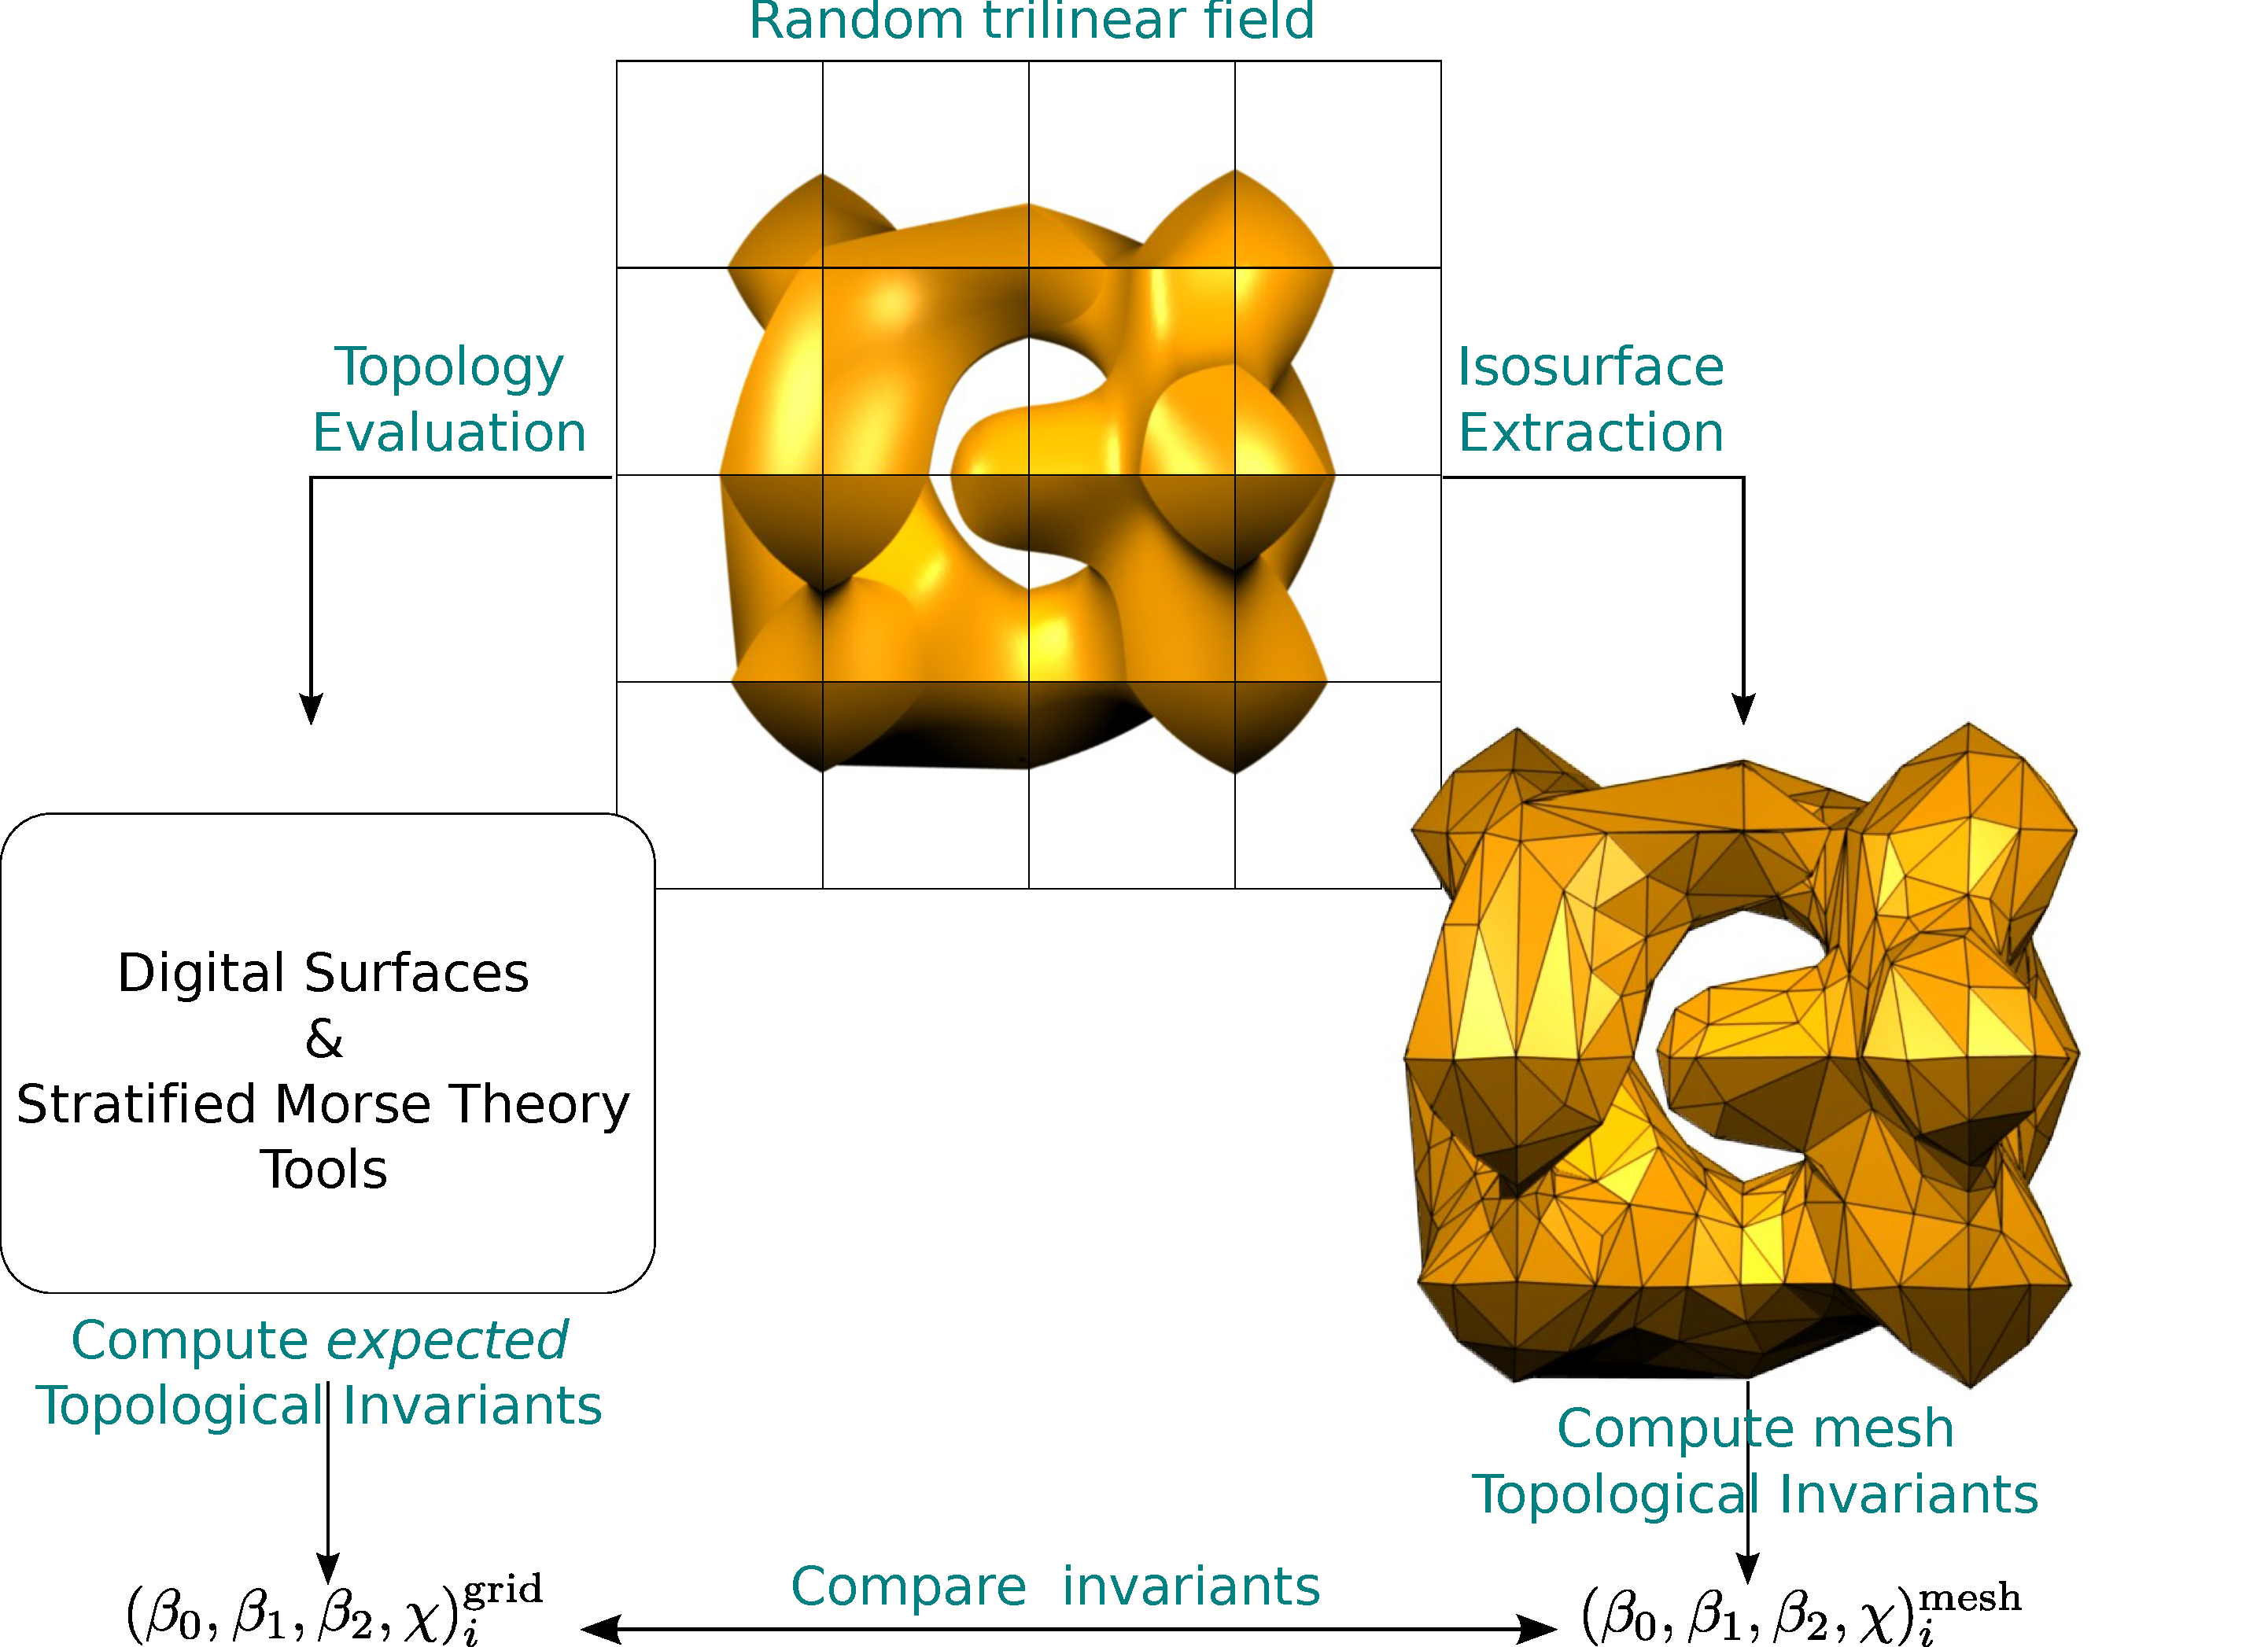
\includegraphics[width=1.0\linewidth,keepaspectratio=true]{chapter3/figures/pipeline.pdf}
\caption{Overview of our topology verification pipeline. First step,
  we generate a random trilinear field and extract a random isosurface
  using the implementation under verification. We then compute the
  \emph{expected} topological invariants from the trilinear field and
  compare them against the invariants obtained from the mesh. We
  provide two simple ways to compute topological invariants from a
  trilinear field based on digital topology (DT) or stratified Morse
  theory (SMT). }
\label{fig:pipeline}
\end{center}
\end{figure}

\section{Mathematical Tools}
\label{sec:math-foundations}

This section describes the mathematical machinery used to derive the
topology verification tools. More specifically, we provide a summary
of the results we need from digital topology and stratified Morse
theory.  A detailed discussion on digital topology can be found in
Stelldinger et al.'s paper~\cite{siqueira:2007}, and Goresky and
MacPherson give a comprehensive presentation of stratified Morse
theory~\cite{Goresky:1988:SMT}.

In Section~\ref{sec:digital-topology}, we describe a method, based on
digital topology, that operates on manifold surfaces without
boundaries and determines the Euler characteristic and Betti numbers
of the level sets. A more general setting of surfaces with boundaries
is handled with tools derived from stratified Morse theory, detailed
in Section~\ref{sec:smt}.  The latter method can only determine the
Euler characteristic of the level set.

Let us start by recalling the definition and some properties of the
Euler characteristic, which we denote by $\chi$. For a compact
2-manifold $\mathcal{M}$, $\chi(\mathcal{M}) = V - E + F$, where $V$,
$E$, and $F$ are the number of vertices, edges, and faces of any finite
cell decomposition of $\mathcal{M}$. If $\mathcal{M}$ is a connected
orientable 2-manifold without boundary, $\chi(\mathcal{M}) = 2 -
2g(\mathcal{M})$, where $g(\mathcal{M})$ is the genus of
$\mathcal{M}$. The Euler characteristic may also be written as
$\chi(\mathcal{M}) = \sum_{i=0}^n(-1)^i \beta_i$, where $\beta_i$ are
the Betti numbers: the rank of the $i$-th homology group of
$\mathcal{M}$.
%$\beta_i = \text{rank} H_i(M)$ is the Betti number and $H_i(M)$ is
%the $i^{th}$ Homology group.
Intuitively, for 2-manifolds, $\beta_0$, $\beta_1$ and $\beta_2$
correspond to the number of connected components, holes and voids
(regions of the space enclosed by the surface) respectively.  If
$\mathcal{M}$ has many distinct connected components, that is,
$\mathcal{M} = \bigcup^n_{i = 1} \mathcal{M}^i$ and $\mathcal{M}^i
\bigcap \mathcal{M}^j = \emptyset$ for $i \neq j$ then
$\chi(\mathcal{M}) = \sum_{i}^n \chi(\mathcal{M}^i)$. More details
about Betti numbers, the Euler characteristic, and homology groups can
be found in Edelsbrunner and Harer's text~\cite{edelsbrunner10}. The
Euler characteristic and the Betti numbers are topological invariants:
two homeomorphic topological spaces will have the same Euler
characteristic and Betti numbers whenever these are well-defined.


\subsection{Digital topology}
\label{sec:digital-topology}

Let $\mathcal{G}$ be an $n\times n \times n$ cubic regular grid with a
scalar $e(s)$ assigned to each vertex $s$ of $\mathcal{G}$ and
$t:\mathbb{R}^3\rightarrow\mathbb{R}$ be the piecewise trilinear
interpolation function in $\mathcal{G}$, that is, ~~$t(x) = t_i(x)$,
where $t_i$ is the trilinear interpolant in the cubic cell $c_i$
containing $x$.
%
Given a scalar value $\alpha$, the set of points satisfying
$t(x)=\alpha$ is called the \emph{isosurface} $\alpha$ of $t$. In what
follows, $t(x)=\alpha$ will be considered a compact, orientable
2-manifold without boundary.
%The complement of a cubic cell $c_i$ is a cubic cell $\bar{c}_i$ such
%that for each vertex $s_i \in c_i$ and $\bar{s}_i \in \bar{c}_i$ we
%have $e(\bar{s}_i) < \alpha$ if $ e(s_i) > \alpha$ and $e(\bar{s}_i)
%> \alpha$ if $ e(s_i) < \alpha$.
We say that a cubic cell $c_i$ of $\mathcal{G}$ is \emph{unambiguous}
if the following two conditions hold simultaneously:
\begin{enumerate}
\item any two vertices $s_a$ and $s_b$ in $c_i$ for which
  $e(s_a)<\alpha$ and $ e(s_b)<\alpha$ are connected by \emph{negative
  edges}, i. e., a sequence of edges $s_as_1,s_1s_2,\ldots,s_ks_b$ in
  $c_i$ whose vertices satisfy $e(s_i)<\alpha$ for $i=1,\ldots, k$ and
\item any two vertices $s_c$ and $s_d$ in $c_i$ for which
  $e(s_c)>\alpha$ and $e(s_d)>\alpha$ are connected by \emph{positive
  edges}, i. e., a sequence of edges $s_cs_1,s_1s_2,\ldots,s_ls_d$ in
  $c_i$ whose vertices satisfy $e(s_i)>\alpha$ for $i=1,\ldots,l$.
\end{enumerate}
 In other words, a cell is unambiguous if all positive vertices form a
 single connected component via the positive edges and, conversely, all
 negative vertices form a single connected component by negative
 edges~\cite{gelder:tog:1994}.  If either property fails to hold, $c_i$ is called \emph{ambiguous}. The top
 row in Figure~\ref{fig:topology_preserving} shows all possible
 unambiguous cases.

\begin{figure}[t]
\begin{center}
\includegraphics[width=1\linewidth,keepaspectratio=true]{chapter3/figures/mi.pdf}
\caption{An illustration of the relation between unambiguous
  isosurfaces of trilinear interpolants and the corresponding digital
  surfaces.  The top row shows all possible configurations of the
  intersection of $t = \alpha$ with a cube $c_j$ for unambiguous
  configurations \cite{lopes:tvcg:2003}.  Each red dot $s_i$ denotes a
  vertex with $e(s_i) < \alpha$. Each image on the top right is the
  complement $\bar{c}_i$ of cases 1 to 4 on the left (cases 5 to 7
  were omitted because the complement is identical to the original
  cube up to symmetry).  The middle row shows the volume reconstructed
  by Majority Interpolation (MI) for configurations 1 to 7 (left) and
  the complements (right) depicted in the top row.  Bottom row shows
  the boundary of the volume reconstructed by the MI algorithm (The
  role of faces that intersect $c_i$ is explained in the proof of
  Theorem~\ref{thm:topological_equivalence_trilinear}).  Notice that
  all surfaces in the top and bottom rows are topological disks. For
  each cube configuration, the boundary of each digital reconstruction
  (bottom row) has the same set of positive/negative connected components as the
  unambiguous configurations (top row).  }
\label{fig:topology_preserving}
\end{center}
\end{figure}

The geometric dual of $\mathcal{G}$ is called the \emph{voxel grid}
associated with $\mathcal{G}$, denoted by $V_{\mathcal{G}}$. More
specifically, each vertex $s$ of $\mathcal{G}$ has a corresponding
voxel $v_s$ in $V_{\mathcal{G}}$, each edge of $\mathcal{G}$
corresponds to a face in $V_{\mathcal{G}}$ (and vice versa), and each
cubic cell in $\mathcal{G}$ corresponds to a vertex in
$V_{\mathcal{G}}$, as illustrated in Figure~\ref{fig:voxelgrid}.  Each
voxel $v_s$ can also be seen as the Voronoi cell associated with $s$.
Scalars defined in the vertices of $\mathcal{G}$ can naturally be
extended to voxels, thus ensuring a single scalar value $e(v_s)$ to
each voxel $v_s$ in $V_{\mathcal{G}}$ defined as $e(s)=e(v_s)$.  As we
shall show, the voxel grid structure plays an
important role when using digital topology to compute topological
invariants of a given isosurface. Before showing that relation,
though, we need a few more definitions.

\begin{figure}[t]
\centering
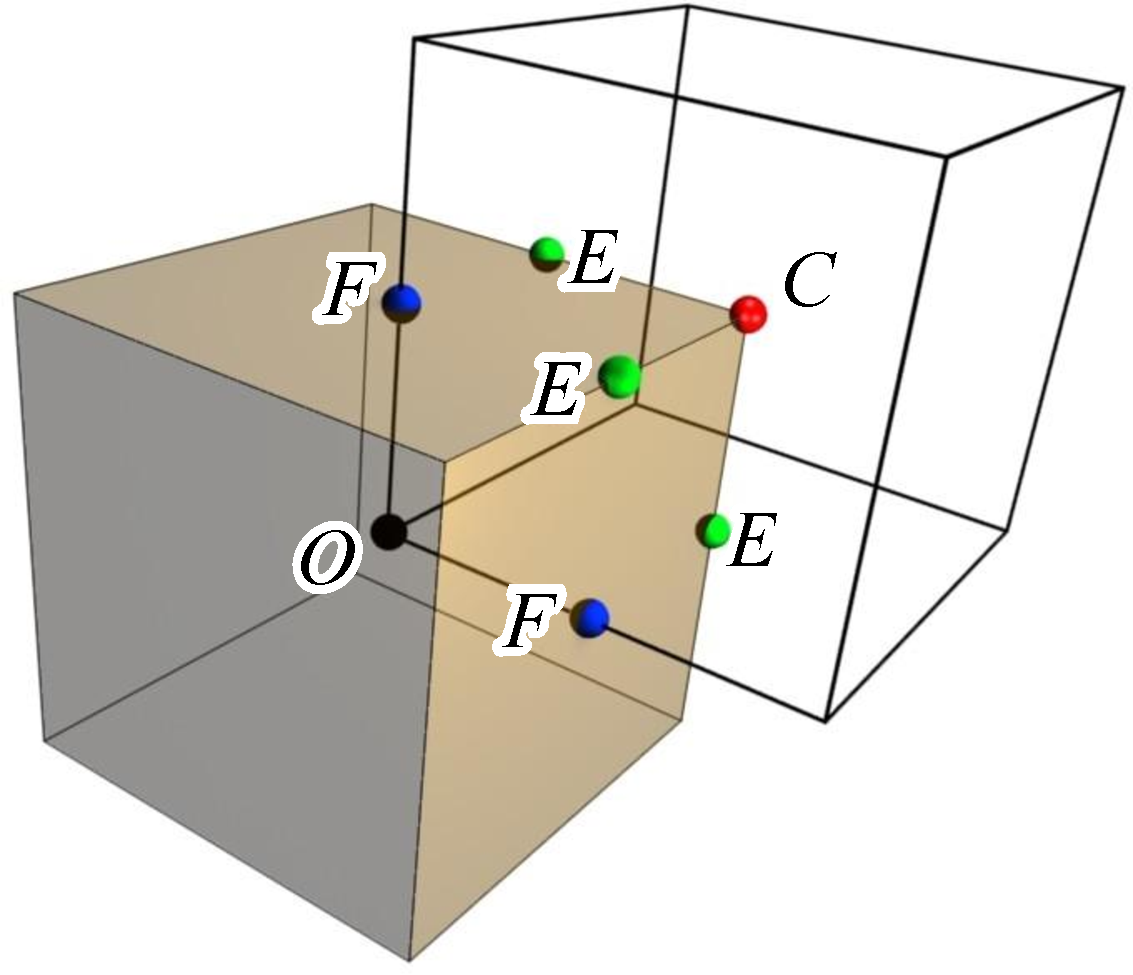
\includegraphics[width=0.35\linewidth]{chapter3/figures/voxel.pdf}
\caption{The four distinct groups of vertices $O, F, E, C$, are
  depicted as black, blue, green, and red points. They are the ``Old'',
  ``Face'', ``Edge,'' and ``Corner'' points of a voxel region
  $V_\mathcal{G}$ (semitransparent cube) respectively. For the sake of
  clarity, we only show a few points.}  
\label{fig:voxelgrid}
\end{figure}


Denote by $\mathcal{G}^\prime$ the $(2n-1)\times (2n-1) \times (2n-1)$ regular grid
obtained from a refinement of $\mathcal{G}$.
%Scalar values can be defined on the vertices of $\mathcal{G}^\prime$
% using the The piecewise trilinear function $t$ defined above, that
% is, if a vertex $s\in\mathcal{G}^\prime$ is also a vertex of
% $\mathcal{G}$ then the value of $e(s)$ is the same as in
% $\mathcal{G}$ otherwise $s$ lies in a cubic cell $c_i$ of
% $\mathcal{G}$ and $e(s)=t(s)$.
Vertices of $\mathcal{G}^\prime$ can be grouped in four distinct sets,
denoted by $O$, $F$, $E$, $C$. The set $O$ contains the vertices of
$\mathcal{G}^\prime$ that are also vertices of $\mathcal{G}$. The sets
$F$ and $E$ contain the vertices of $\mathcal{G}^\prime$ lying on the
center of faces and edges of the voxel grid $V_{\mathcal{G}}$,
respectively. Finally, $C$ contains all vertices of $V_{\mathcal{G}}$.
Figure~\ref{fig:voxelgrid} illustrates these sets.

Consider now the voxel grid $V_{\mathcal{G^\prime}}$ dual to the
refined grid $\mathcal{G}^\prime$.  Given a scalar value $\alpha$, the
\emph{digital object} $\mathcal{O}_\alpha$ is the subset of voxels $v$
in $V_{\mathcal{G^\prime}}$ such that $v\in\mathcal{O}_\alpha$ if at
least one of the criteria below are satisfied:
\begin{itemize}
\item $v\in O$ and $e(v)\leq\alpha$
\item $v\in F$ and both neighbors of $v$ in $O$ have scalars less than
  (or equal to) $\alpha$
\item $v\in E$ and at least $4$ of the $8$ neighbors of $v$ in $O\cup
  F$ have scalars less than (or equal) $\alpha$
\item $v\in C$ and at least $12$ of the $26$ neighbors of $v$ in
  $O\cup F\cup E$ have scalars less than (or equal) $\alpha$
\end{itemize}
The description above is called Majority Interpolation (MI) 
(Algorithm~\ref{alg:majority-interpolation}), and it allows us to compute
the voxels that belong to a digital object $\mathcal{O}_\alpha$.
%satisfying the above criteria, we use Majority Interpolation (MI), a
%procedure illustrated in Figure~\ref{alg:majority-interpolation}.
%cscheid: I removed the sentence below, because it was in the way of
%the rest of the exposition here. It belongs in the discussion More
%importantly, MI is a simple algorithm, an essential requirement in
%the context of verification.
The middle row of Figure~\ref{fig:topology_preserving} shows all
possible cases for voxels picked by the MI algorithm (notice the
correspondence with the top row of the same figure).

\begin{algorithm}[t]
\begin{codebox}
\Procname{$\proc{MajorityInterpolation}(\mathcal{G},\alpha)$}
%\li \Comment Let $S'$ be $S$ with resolution doubled
\li \Comment Let $O$, $F$, $E$ and $C$ be the subset of vertices 
\zi ~~~in $\mathcal{G}^\prime$ as described in
subsection~\ref{sec:digital-topology}. %an old, face, edge and corner point
%\zi  respectively (Definition \ref{dff:majority-interpolation}).
\li \Comment Let $\mathpzc{N}(s, \star)$ be the set of neighbors of
$s\in\mathcal{G}^\prime$ in the \zi ~~~ set $\star$, where $\star =
\{O, F, E, C\}$, with associate scalar \zi ~~~ less than $\alpha$
%\zi of $s \in S'$ inside $p = 0$
\li \For $s \in \mathcal{G}^\prime$
\li     \Do  	\If $s \in O$ \bf or
\li		    $s \in \proc{F}$ and $|\mathpzc{N}(s, O)| = 2$ \bf or
\li			  $s \in E$ and $|\mathpzc{N}(s, O)+\mathpzc{N}(s, F)| 
\geqslant 4$ \bf or
\li		    $s \in \proc{C}$ and $|\mathpzc{N}(s, O)+\mathpzc{N}(s,
F)+\mathpzc{N}(s,E)| \geqslant 12$
\li		\Then Select voxel $v_s$
		\End
	\End
\li \Return $\mathcal{O}_\alpha$
\end{codebox}
\caption{Voxel selection using Majority Interpolation (MI).
}
\label{alg:majority-interpolation}
\end{algorithm}

The importance of $\mathcal{O}_\alpha$ is two-fold. First, the
boundary surface of the union of the voxels in $\mathcal{O}_\alpha$,
denoted by $\partial\mathcal{O}_\alpha$ and called a \emph{digital
  surface}, is a $2$-manifold (See the proof by Stelldinger et
al.~\cite{siqueira:2007}). Second, the genus of
$\partial\mathcal{O}_\alpha$ can be computed directly from
$\mathcal{O}_\alpha$ using the algorithm proposed by Chen and Rong
\cite{LiChen:2008} (Algorithm~\ref{alg:compute-invariant}). As the
connected components of $\mathcal{O}_\alpha$ can also be easily
computed and isolated, one can calculate the Euler characteristic of
each connected component of $\mathcal{O}_\alpha$ from the formula
$\chi = 2 - 2g$ and thus $\beta_0$, $\beta_1$, and $\beta_2$.
% cscheid: We should say how that is done here.

The voxel grid $V_{\mathcal{G^\prime}}$ described above allows us to
compute topological invariants for any digital surface
$\partial\mathcal{O}_\alpha$. However, we so far do not have any
result relating $\partial\mathcal{O}_\alpha$ to the isosurface
$t(x)=\alpha$.  The next theorem provides the connection.

\begin{thm}
Let $\mathcal{G}$ be an $n\times n\times n$ rectilinear grid with scalars
associated with each vertex of $\mathcal{G}$ and $t$ be the piecewise trilinear 
function defined on $\mathcal{G}$, such that the isosurface $t(x)=\alpha$ is a
2-manifold without boundary. If no cubic cell of $\mathcal{G}$ is
ambiguous with respect to $t(x)=\alpha$, then $\partial\mathcal{O}_\alpha$
is homeomorphic to the isosurface $t(x)=\alpha$.
\label{thm:topological_equivalence_trilinear}
\end{thm}
{\bf Proof:} Given a cube $c_i \subset \mathcal{G}$ and an isosurface
 $t = \{x \;|\; t(x) = \alpha\}$, let $t_i = t \cap c_i$.  Similarly,
denote
\[\partial \mathcal{O}_i =  cl_{\mathbb{R}^3} \left( (\partial \mathcal{O}_\alpha \cap c_i) - \partial c_i  \right),\]
where $cl_{\mathbb{R}^3}$ denotes the closure operator. We note that
$\partial \mathcal{O}_i$ is a 2-manifold for all $i$
\cite{SPB04,siqueira:2007}.  There are two main parts to the proof
presented here. For each $i$,
\begin{enumerate}
%\vspace{-0.1in}
\item the 2-manifolds $t_i$ and $\partial \mathcal{O}_i$ are homeomorphic; and
%\vspace{-0.1in}
\item both $t_i$ and $\partial \mathcal{O}_i$ cut the same edges and faces of $c_i$.
%\vspace{-0.1in}
\end{enumerate}

Since $t$ is trilinear, no level-set of $t$ can intersect an edge more
than once. Hence, if $c_i$ is not ambiguous, $t_i$ is exactly one of
the cases 1 to 7 in the top row of
Figure~\ref{fig:topology_preserving}~\cite{lopes:tvcg:2003},
either a topological disk or the empty set.  
%
%The digital reconstruction of each unambiguous case is shown in the
%middle row of Figure \ref{fig:topology_preserving}.
%
Each case in the top row of Figure \ref{fig:topology_preserving} is
the unambiguous input for the MI algorithm to produce the voxel
reconstruction shown in the middle row, where the boundaries of each of
these voxel reconstructions are shown in the bottom row.
%
By inspection, we can verify
that the boundary of the digital reconstruction $\partial
\mathcal{O}_i$ (bottom row of Figure \ref{fig:topology_preserving}) is
also a disk for all possible unambiguous cases and complement cases.
Hence, for each $i$, the 2-manifolds $\partial \mathcal{O}_i$ and
$t_i$ are homeomorphic.
%
Then, for each $i$, both $\partial \mathcal{O}_i$ and $t_i$ cut the same
set of edges and faces of $c_i$. Again, we can verify this for all possible $i$
by inspecting the top and bottom rows in Figure \ref{fig:topology_preserving}, respectively.
%
Finally, we apply the Pasting Lemma~\cite{Munkres} across
neighboring surfaces $\partial \mathcal{O}_i$ and $\partial \mathcal{O}_j$ in order to
establish the homeomorphism between $\partial \mathcal{O}_\alpha$
and $t$.
$\Box$
% cscheid: I don't think the Pasting Lemma applies here. The pasting
% lemma is used to create continuous functions in unions of sets by
% combining continuos functions in the subsets and using the natural
% topology. This is not what we need here - since we are trying to
% relate different subsets (the digital reconstructions and the level
% sets of the scalar field) by homeomorphisms. We need something
% stronger. Our other paper has a lemma that might be too strong, but
% is certainly sufficient.

This proof provides a main ingredient for
the verification method in Section~\ref{sec:manufactured}. Crucially, 
we will show how to manufacture a complex solution that
unambiguously crosses every cubic cell of the grid. Since we have
shown the conditions for which the digital surfaces and the level sets
are homeomorphic, any topological invariant will have to be the
same for both surfaces.

\subsection{Stratified Morse Theory}
\label{sec:smt}
The mathematical developments presented above allow us to compute the
Betti numbers of any isosurface of the piecewise trilinear
interpolant.  However, they require isosurfaces without boundaries.
In this section, we provide a mechanism to compute the Euler
characteristic of any regular isosurface of the piecewise trilinear
interpolant through an analysis based on critical points, which can be
used to verify properties of isosurfaces with boundary components.  We
will use some basic machinery from stratified Morse theory (SMT),
following the presentation of Goresky and MacPherson's
monograph~\cite{Goresky:1988:SMT}.
%We follow the presentation of a separate
%report~\cite{scheidegger:techreport:2010} (submitted as supplementary
%material), which provides a mechanism to compute the Euler
%characteristic of piecewise trilinear isosurfaces using a
%mathematical framework derived from Stratified Morse Theory (SMT)
%\cite{scheidegger:techreport:2010}.

Let $f$ for now be a smooth function with isolated critical points
$p$, where $\nabla f(p) = 0$.  From classical Morse theory, the
topology of two isosurfaces $f(x)=\alpha$ and $f(x)=\alpha+\epsilon$
differs only if the interval $[\alpha, \alpha + \epsilon]$ contains a
critical value ($f(p)$ is a critical value iff $p$ is a critical
point). Moreover, if $\varepsilon_p$ is a small neighborhood around
$p$ and $L^-(p)$ and $L^+(p)$ are the subset of points on the boundary
of $\varepsilon_p$ satisfying $f(x)<f(p)$ and $f(x)>f(p)$
respectively, then the topological change from the isosurface
$f(x)=f(p)-\epsilon$ to $f(x)=f(p)+\epsilon$ is characterized by
removing $L^-(p)$ and attaching $L^+(p)$. Thus, changes in the Euler
characteristic, denoted by $\Delta\chi(p)$, are given by:
\begin{equation}
\Delta\chi(p) = \chi(L^+(p)) - \chi(L^-(p)).
\label{eq:deltachi}
\end{equation}
% \noindent where $\chi(L^-(p))$ and $\chi(L^+(p))$ are the Euler characteristic of $L^-(p)$ and $L^+(p)$,
% respectively. 
\noindent For a smooth function $f$, the number of negative eigenvalues of the
Hessian matrix determines the index of a critical point $p$, and the
four cases give the following values for $\chi(L^-(p))$
and $\chi(L^+(p))$:
%In the smooth scenario, $\chi(L^-(p))$ and $\chi(L^+(p))$
%can be inferred from the number of negative eigenvalues of the Hessian
%matrix of $f$ in $p$, and we have four distinct cases:
\begin{center}
\begin{tabular}{c|c|c|c|c}
& min & saddle-1 & saddle-2 & max \\
\hline
$\chi(L^-(p))$ & 0 & 2 & 0 & 2 \\ 
$\chi(L^+(p))$ & 2 & 0 & 2 & 0
\end{tabular}
\end{center}
The above formulation is straightforward but unfortunately cannot be directly applied to
functions appearing in either piecewise trilinear interpolations or
isosurfaces with boundary, both of which
appear in some of the isosurfacing algorithms with guaranteed
topology. Trilinear interpolants are not smooth across the faces
of grid cells, so the gradient is not well-defined there. Identifying the
critical points using smooth Morse theory is then
problematic. Although arguments based on smooth Morse
theory have appeared in the
literature~\cite{Weber:2002:ESF}, there are complications. For
example, the scalar field in a node
of the regular grid might not have \emph{any} partial
derivatives. Although one can still argue about the
intuitive concepts of minima and maxima around a non-differentiable point,
configurations such as saddles are more problematic, since their
topological behavior is different depending on whether they are on the
boundary of the domain. It is 
important, then, to have a mathematical tool which makes predictions
regardless of the types of configurations, and SMT is one such theory.

Intuitively, a \emph{stratification} is a partition of a
piecewise-smooth manifold such that each subset, called a
\emph{stratum}, is either a set of discrete points or has a smooth
structure.  In a regular grid with cubic cells, the stratification we
propose will be formed by four sets (the strata), each one a (possibly
disconnected) manifold.  The \emph{vertex set} contains all vertices
of the grid. The \emph{edge set} contains all edge interiors, the
\emph{face set} contains all face interiors, and the \emph{cell set}
contains all cube interiors. We illustrate the concept for the 2D case
in Figure~\ref{fig:stratification}.  The important property of the
strata is that the level sets of $f$ restricted to each stratum are
smooth (or lack any differential structure, as in the vertex-set). In
SMT, one applies standard Morse theory on each stratum, and then
combines the partial results appropriately.

\begin{figure}[t]
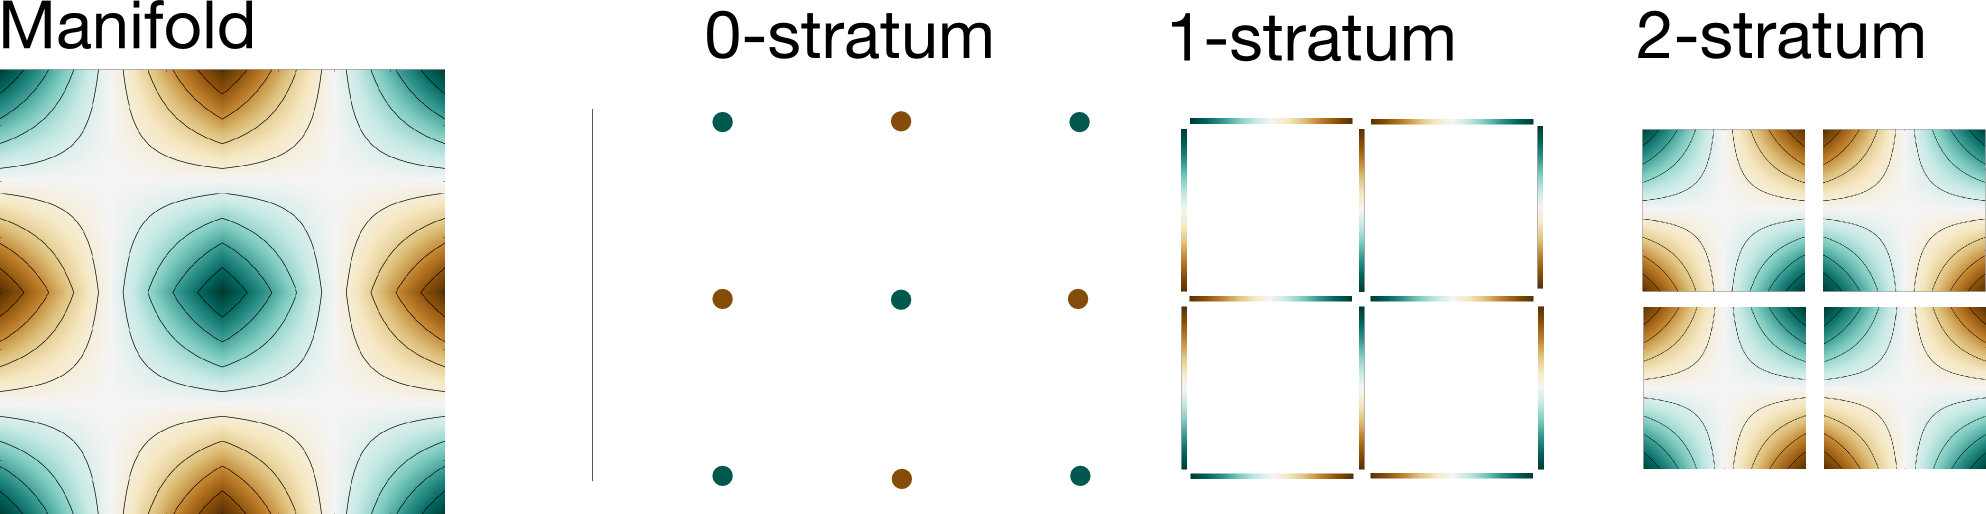
\includegraphics[width=\linewidth]{chapter3/figures/stratification.png}
\caption{\label{fig:stratification}An illustration of a
  piecewise-smooth immersed 2-manifold. The colormap illustrates the
  value of each point of the scalar field. Notice that although the manifold
  itself is not everywhere differentiable, each stratum is itself an open
  manifold that is differentiable.}
\end{figure}

The set of points with zero gradient (computed on each stratum), which
SMT assumes to be isolated, are called the \emph{critical points} of
the stratified Morse function. In addition, every point in the vertex
set is considered critical as well. One major difference between SMT
and the smooth theory is that some critical points do not actually
change the topology of the level sets. This is why considering all
grid vertices as critical does not introduce any practical problems:
most grid vertices of typical scalar fields will be \emph{virtual
  critical points}, {\em i.e.}, points which do not change the Euler
characteristic of the surface. Carr and Snoeyink use a
related concept (which they call ``potential critical points'') in
their state-machine description of the topology of
interpolants~\cite{CS08}.

Let $\mathcal{M}$ be the stratified grid described above.  It can be
shown that if $p$ is a point in a $d$-dimensional stratum of
$\mathcal{M}$, it is always possible to find a $(3-d)$-dimensional
submanifold of $\mathcal{M}$ (which might straddle many strata) that
meets transversely the stratum containing $p$, and whose intersection
consists of only $p$ (one way to think of this $(3-d)$-manifold is as a ``topological orthogonal
complement'').  In this context, we can define a small neighborhood
$T_\varepsilon(p)$ in the strata containing $p$ and the \emph{lower
  tangential} link $T_L^-(p)$ as the set of points in the boundary of
$T_\varepsilon(p)$ with scalar values less than that in $p$.
\begin{wrapfigure}{r}{3cm}
\centering
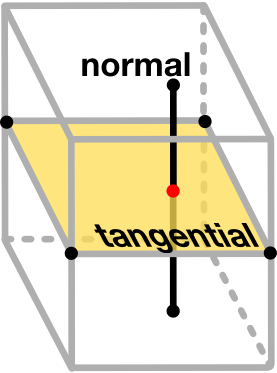
\includegraphics[width=2.0cm,keepaspectratio=true]{chapter3/figures/ilustration.png}
\end{wrapfigure}
Similarly we can define the \emph{upper tangential} link $T_L^+(p)$ as
the set of points in the boundary of $T_\varepsilon(p)$ with scalar
value higher than that at $p$.  \emph{Lower normal} $N_L^-(p)$ and
\emph{upper normal} $N_L^+(p)$ links are analogous notions, but the
lower and upper links are taken to be subsets of $N_\varepsilon(p)$,
itself a subset of the $(3-d)$-dimensional submanifold transverse to
the stratum of $p$ going through $p$.  The definitions above are needed
in order to define the \emph{lower stratified link} and \emph{upper
  stratified link}, as follows: given $T_\varepsilon(p),\,
T_L^-(p),\,N_\varepsilon(p)$ and $N_L^-(p)$, the \emph{lower
  stratified Morse link} (and similarly for upper stratified link) is
given by
\begin{equation}
L^-(p) = (T_\varepsilon(p) \times N_L^-(p)) \cup (N_\varepsilon(p)
\times T_L^-(p)) \label{eq:lowerstratifiedlink}.
\end{equation}
These definitions allow us to classify critical points even in the non-smooth scenario.
They let us compute topological changes with
the same methodology used in the smooth case. In other words, when a
scalar value $\alpha$ crosses a critical value $\alpha_p$ in a
critical point $p$, the topological change in the isosurface is
characterized by removing $L^-(p)$ and attaching $L^+(p)$, affecting
the Euler characteristic as defined in Equation~\ref{eq:deltachi}.%\cite{?}.

The remaining problem is how to determine $\chi(L^-(p))$ and
$\chi(L^+(p))$. 
Recalling that $\chi(A \cup B) = \chi(A) + \chi(B) - \chi(A \cap B)$,
$\chi(A\times B)=\chi(A)\chi(B)$, and $\chi(T_\varepsilon)=\chi(N_\varepsilon)=1$ (we are omitting 
the point $p$) we have:
\begin{equation}
\begin{array}{l}
\chi(L^-) = \chi(T_\varepsilon \times N_L^- \cup N_\varepsilon \times T_L^-) \\
    \qquad  = \chi(N_L^-) + \chi(T_L^-) - \chi(T_\varepsilon \times N_L^- \cap N_\varepsilon \times T_L^-)
\end{array}
\end{equation}
Now, we can define $T_\varepsilon = T_L^- \cup T_r,\, T_L^- \cap T_r =
\emptyset$ and similarly for $N_\varepsilon$ and $N_L^-$.  Then,
expand the partitions and products, and distribute the intersections
around the unions, noticing all but one of intersections will be
empty:
\begin{eqnarray*}
T_\varepsilon \times N_L^- \cap N_\varepsilon \times T_L^- \hspace{-8.0px} &=& \hspace{-8.0px} ((T_r \cup T_L^-) \times N_L^-) \cap ((N_r \cup N_L^-) \times T_L^-) \\
\hspace{-8.0px} &=& \hspace{-8.0px} ((T_r \times N_L^-) \cup (T_L^- \times N_L^-)) \cap \\
\hspace{-8.0px} && \hspace{-8.0px}((N_r \times T_L^-) \cup (N_L^- \times T_L^-)) \\
\hspace{-8.0px} &=& \hspace{-8.0px}N_L^- \times T_L^-
\end{eqnarray*}
Therefore:
\begin{eqnarray*}
\chi(T_\varepsilon \times N_L^- \cap N_\varepsilon \times T_L^-) &=& \chi(N_L^- \times T_L^-) \\
&=& \chi(N_L^-)\chi(T_L^-)
\end{eqnarray*}
which gives the final result
\begin{equation}
\chi(L^-) = \chi(N_L^-)+\chi(T_L^-)-\chi(N_L^-)\chi(T_L^-) \label{eq:lowerchi}.
\end{equation}

The same result is valid for $\chi(L^+)$, if we replace the 
superscript `$-$' by `$+$' in Equation~\ref{eq:lowerchi}. If $T_L^-$ or
$T_L^+$ are one-dimensional, then we are done. If not, then we can
recursively apply the same equation to $T_L^-$ and $T_L^+$ and look at
progressively lower-dimensional strata until we reach
$T_\varepsilon(p)$ and $N_\varepsilon(p)$ given by $1$-disks. The
lower and upper links for these \mbox{$1$-disks} will always be
discrete spaces with zero, one, or two points, for which $\chi$ is
simply the cardinality of the set.

In some cases, the Euler characteristic of the lower and upper link
might be equal. Then, $\chi(L^-(p)) = \chi(L^+(p))$, and
$\Delta\chi(p) = 0$. These cases correspond to the virtual critical
points mentioned above.
%, that is, critical points which do not change
%the Euler characteristic of the surface.
%
Critical points in the interior of cubic cells are handled by the
smooth theory, since in that case the normal Morse data is
0-dimensional. This implies that the link will be an empty set with
Euler characteristic zero. So, by Equation~\ref{eq:lowerchi},
$\chi(L^-) = \chi(T_L^-)$. Because the restriction of the scalar field
to a grid edge is a linear function, no critical point can appear
there. As a result, the new cases are critical points occurring at
vertices or in the interior of faces of the grid.  For a critical
point $p$ in a vertex, stratification can be carried out recursively,
using the edges of the cubes meeting in $p$ as tangential and normal
submanifolds. Denoting by $n_{l1},n_{l2},n_{l3}$ the number of
vertices adjacent to $p$ with scalar value less than that of $p$ in
each Cartesian coordinate direction, Equation~(\ref{eq:lowerchi})
gives:
\begin{equation}
\chi(L^-(p)) = n_{l1}+n_{l2}+n_{l3} - n_{l1}(n_{l2}+n_{l3})
\end{equation}
$\chi(L^+(p))$ can be computed similarly, but considering the number of neighbors of $p$ in each Cartesian 
direction with scalars higher than that of $p$.

If $p$ is a critical point lying in a face $r$ of a cube, we consider
the face itself as the tangential submanifold and the line segment
$r^\perp$ orthogonal to $r$ through $p$ the normal submanifold.
Recursively, the tangential submanifold can be further stratified in
two $1$-disks (tangential and normal).  Denote by $n_l$ the number of
ends of $r^\perp$ with scalar value less than that of $p$. Also,
recalling that the critical point lying in the face $r$ is necessarily
a saddle, thus having two face corners with scalar values less and two
higher than that of $p$, Equation~(\ref{eq:lowerchi}) gives:
\begin{equation}
\chi(L^-(p)) = n_l+2 - 2\,n_l
\end{equation}
Analogously, we can compute $\chi(L^+(p)) = n_u+2 - 2\,n_u$ where
$n_u$ is the number of ends of $r^\perp$ with scalar value higher than
that of $p$.

A similar analysis can be be carried out for every type of critical
point, regardless of whether the point belongs to the interior of a
grid cell (and so would yield equally well to a smooth Morse theory
analysis), an interior face, a boundary face, or a vertex of any
type. The Euler characteristic $\chi_\alpha$ of any isosurface with
isovalue $\alpha$ is simply given as:
\begin{equation}
\chi_\alpha = \sum_{p_i\in C_\alpha} \Delta\chi(p_i)
\label{ref:chis}
\end{equation}
where $C_\alpha$ is the set of critical points with critical values less than $\alpha$.

It is worth mentioning once again that, to the best of our knowledge,
no other work has presented a scheme which provides such a simple
mechanism for computing the Euler characteristic of level sets of
piecewise-smooth trilinear functions. Compare, for example, the case
analyses and state machines performed separately by
Nielson~\cite{Nielson03onmarching}, by Carr and Snoeyink~\cite{CS08},
and by Carr and Max~\cite{10.1109/TVCG.2009.10}. In contrast, we can recover an
(admittedly weaker) topological invariant by a much simpler
argument. In addition, this argument already generalizes (trivially
because of the stratification argument) to arbitrary dimensions,
unlike the other arguments in the literature.


\section{Manufactured Solution Pipeline}
\label{sec:manufactured}

We now put the pieces together and build a pipeline for topology 
verification using the results presented in Section~\ref{sec:math-foundations}. 
In the following sections, the procedure called $\proc{Isosurfacing}$ refers to the
isosurface extraction technique under verification.
$\proc{InvariantFromMesh}$ computes topological invariants of a simplicial
complex. 
%Section \ref{sec:discussion} compares the verification pipelines using
%Digital Topology and Stratified Morse Theory.


\subsection{Consistency}
\label{sec:consistency-verification}

As previously mentioned, MC-like algorithms which use
disambiguation techniques are expected to generate PL manifold isosurfaces no matter how complex 
the function sampled in the vertices of the regular grid. 
In order to stress the consistency test, we generate a random scalar field with values in the
interval $[-1,1]$ and extract the isosurface with isovalue $\alpha=0$
(which is all but guaranteed not to be a critical value) using a
given isosurfacing technique, subjecting the 
resulting triangle mesh to the consistency verification. This process
is repeated a large number of times, and  
%
if the implementation fails to
produce \mbox{PL manifolds} for all cases, then the counterexample
provides a documented starting point for debugging. If it passes the
tests, we consider the implementation verified.
% (in the sense of analyzed predicted behavior) for all test cases to which
% it has been applied, increasing our confidence in the stated properties

\subsection{Verification using Stratified Morse Theory}
\label{subsec:smt-verify}

We can use the formulation described in Section~\ref{sec:smt} to
verify isosurfacing programs which promise to match the
topology of the trilinear interpolant.
The SMT-based verification procedure is summarized in
Algorithm~\ref{alg:manufactured-solutions-smt}. The algorithm 
has four main steps. A random scalar field with node values in the
interval $[-1,1]$ is initially created. Representing the trilinear
interpolation in a grid cell by $f(x,y,z) = axyz + bxy + cxz + dyz + ex + fy + gz + h$,
the internal critical points are given by:
\[\begin{array}{ccc}
t_x = (d \Delta_x \pm \sqrt{\Delta_x \Delta_y \Delta_z})/({a \Delta_x})\\
t_y = (c \Delta_y \pm \sqrt{\Delta_x \Delta_y \Delta_z})/({a \Delta_y})\\
t_z = (b \Delta_z \pm \sqrt{\Delta_x \Delta_y \Delta_z})/({a \Delta_z}),
\end{array}\]
%% \begin{eqnarray*}
%% t_x &=&  \\
%% t_y &=&  \\
%% t_z &=&  
%% \end{eqnarray*}
\noindent where $\Delta_x = bc-ae$, $\Delta_y = bd-af$, and $\Delta_z
= cd-ag$~\cite{Pascucci03}.  Critical points on faces of the cubes are found by setting
$x,y$ or $z$ to either 0 or 1, and solving
the quadratic equation.  
If the solutions lie outside the unit cube $[0, 1]^3$, they are not
considered critical points, since they lie outside the domain of the cell. The scalar field
is regenerated if any degenerate critical point is detected (these
can happen if either the random values in a cubic cell have, by chance, the same value or when 
$\Delta_x$, $\Delta_y$ or $\Delta_z$ are zero). In order
to avoid numerical instabilities, we also regenerate the scalar field
locally if any internal critical point lies too close to the border of
the domain (that is, to an edge or to a face of the cube).

\begin{algorithm}[t]
\begin{codebox}
\Procname{$\proc{MMS-SMT}(\mathcal{G})$}
\li \Comment Let the input $\mathcal{G}$ be $n \times n \times n$ rectilinear grid
\li \For $i \gets 1$ \To $\#$tests
\li     \Do $\mathcal{G} \gets$ randomly sampled $n \times n \times n$ grid \label{alg:mms:sampling}
\li         $\id{CPs} \gets \proc{ComputeCriticalPoints}(\mathcal{G})$
\li         \If $p \in CPs$ is degenerate \kw{or}
\li		$p$ is an internal saddle close to edges or faces
\li         	\Then $\proc{GoTo}$ \ref{alg:mms:sampling} \label{alg:mms:goto-smt}
\li         \Else $K \gets \proc{Isosurfacing}(\mathcal{G})$
\li         	  $(\chi^v)_i \gets \proc{InvariantFromCPs}(\mathcal{G})$
\li         	  $(\chi^k)_i \gets \proc{InvariantFromMesh}(K)$
	    \End
\li Compare $(\chi^v)_i$ and $(\chi^k)_i$
      \End
\end{codebox}
\caption{Overview of the method of manufactured solutions (MMS) using
stratified Morse theory. \proc{InvariantFromCPs} is computed using Equation
\ref{ref:chis}. The method either fails to match the expected topology, in
which case $\mathcal{G}$ is provided as a counterexample, or
succeeds otherwise.}
\label{alg:manufactured-solutions-smt}
\end{algorithm}

The third step computes the Euler characteristic of a set of
isosurfaces with random isovalues in the interval $[-1, 1]$ using the
theory previously described, jointly with Equation~\ref{ref:chis}.  In
the final step, the triangle mesh $M$ approximating the isosurfaces is
extracted using the algorithm under verification, and $\chi(M) = V(M)
- E(M) + F(M)$, where $V(M),E(M)$, and $F(M)$ are the number of
vertices, edges, and triangles. If the Euler characteristic computed
from the mesh does not match the one calculated via
Equation~\ref{ref:chis}, the verification fails. We carry out the
process a number of times, and implementations that pass the tests are
less likely to contain bugs.

\subsection{Verification using Digital Topology}
\label{subsec:ds-verify}

Algorithm~\ref{alg:manufactured-solutions-digital-surfaces} shows the
verification pipeline using the MI algorithm, and
Figure~\ref{fig:trilinear-field} depicts the refinement process. Once
again a random scalar field, with potentially many ambiguous cubes, is
initially generated in the vertices of a grid $\mathcal{G}$.  The
algorithm illustrated in
Algorithm~\ref{alg:manufactured-solutions-digital-surfaces} is applied to
refine $\mathcal{G}$ so as to generate a new grid
$\tilde{\mathcal{G}}$ which does not have ambiguous cells. If the
maximum number of refinement is reached and ambiguous cells still
remain, then the process is restarted from scratch.  Notice that cube
subdivision does not need to be uniform.  For instance, each cube may
be refined using a randomly placed new node point or using $t_i$'s
critical points, and the result of the verification process still
holds.  This is because Theorem
$\ref{thm:topological_equivalence_trilinear}$ only requires $c_i$ to
be unambiguous.
%This shows us that the reliability of this verification process depends 
%only on key concepts with other steps performed in
%possibly many different ways. 
For simplicity, in this work we refine $\mathcal{G}$ uniformly
doubling the grid resolution in each dimension.

\begin{algorithm}[t]
\begin{codebox}
\Procname{$\proc{MMS-DS}(\mathcal{G})$}
\li \Comment Let the input $\mathcal{G}$ be a $n \times n \times n$ rectilinear grid
\li \For $i \gets 1$ \To $\#$tests
\li     \Do  $\mathcal{G} \gets$ randomly sampled $n \times n \times n$ grid \label{alg:mms:sampling2}
\li         $\tilde{\mathcal{G}} \gets \proc{RefineAndResample}(\mathcal{G})$
\li         \If $\tilde{\mathcal{G}}$ has ambiguous cubes
\li         	\Then $\proc{GoTo}$ \ref{alg:mms:sampling2} \label{alg:mms:goto-dt}
			\End
\li         $\mathcal{O} \gets
\proc{MajorityInterpolation}(\tilde{\mathcal{G}})$
\li 		  $K \gets \proc{Isosurfacing}(\mathcal{G})$
\li         	  $(\beta_0^v, \beta_1^v,\beta_2^v)_i \gets
\proc{InvariantFromDS}(\partial {\mathcal{O}})$
\li         	  $(\beta_0^k, \beta_1^k,\beta_2^k)_i \gets
\proc{InvariantFromMesh}(K)$
\li Compare $(\beta_0^v, \beta_1^v,\beta_2^v)_i$ and $(\beta_0^k, \beta_1^k,\beta_2^k)_i$
	    \End
      \End
\end{codebox}
\caption{Overview of the method of manufactured solutions (MMS) using digital
topology. The method either fails to match the expected topology, in
which case $\mathcal{G}$  is provided as a counterexample, or
succeeds otherwise.}
\label{alg:manufactured-solutions-digital-surfaces}
\end{algorithm}

\begin{figure}[t]
\centering
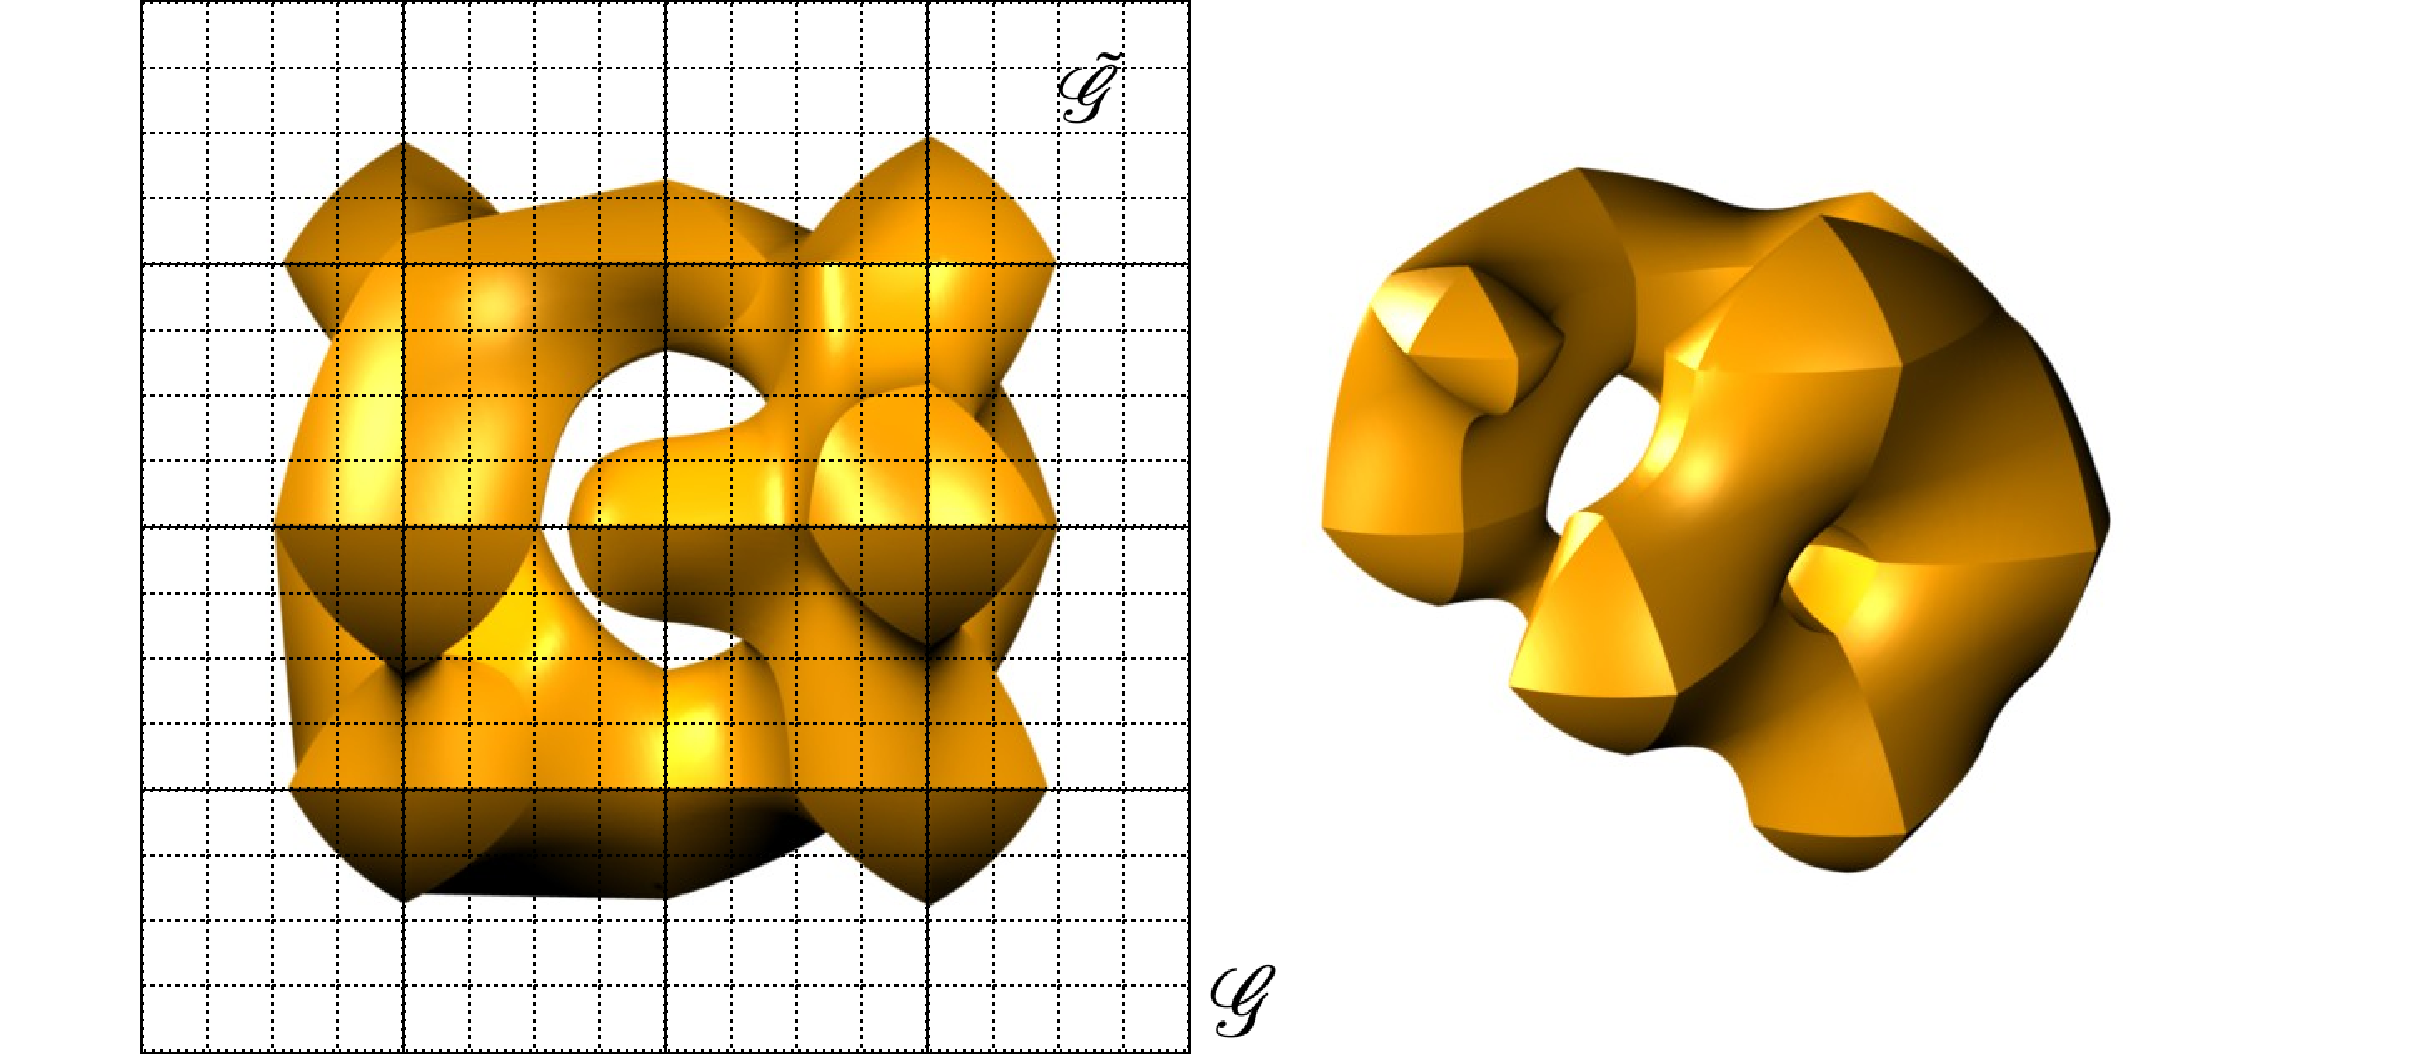
\includegraphics[width=1.0\linewidth,keepaspectratio=true]
{chapter3/figures/trilinear-field.pdf}
\caption{Our manufactured solution is given by $t(x) = \alpha$. $\mathcal{G}$ is
depicted in solid lines while $\tilde{\mathcal{G}}$ is shown in dashed lines.
$\tilde{\mathcal{G}}$ is a uniform subdivision of $\mathcal{G}$. The trilinear
surfaces $t_i$ are defined for each cube
$c_i \in \mathcal{G}$ and resampled in $c'_j \in \tilde{\mathcal{G}}$.
The cubes in the center of $\mathcal{G}$ have four maxima each
(left) and thus induce complicated topology. The final
isosurface may have several tunnels and/or connected
components even for coarse $\mathcal{G}$ (right). }
\label{fig:trilinear-field}
\end{figure}

Scalars are assigned to the new vertices of $\tilde{\mathcal{G}}$ (the ones not in $\mathcal{G}$) by trilinearly 
interpolating
from scalars in $\mathcal{G}$, thus ensuring that $\mathcal{G}$ and  $\tilde{\mathcal{G}}$ have
exactly the same scalar field~\cite{Nielson03onmarching}.
As all cubic cells in $\tilde{\mathcal{G}}$ are unambiguous, Theorem \ref{thm:topological_equivalence_trilinear} guarantees 
the topology of the digital surface $\partial\mathcal{O}_\alpha$
obtained from $\tilde{\mathcal{G}}$ is equivalent to 
that of $t(x)=\alpha$. Algorithm \proc{InvariantFromDS} computes
topological invariants of
$\partial\mathcal{O}_\alpha$ using the scheme discussed in
Section~\ref{sec:digital-topology}. In this context, \proc{InvariantFromDS} is
the algorithm illustrated in Algorithm~\ref{alg:compute-invariant}.
Surfaces with boundary are avoided by assigning the scalar value $1$ to every vertex in the
boundary of $\mathcal{G}$.

\begin{algorithm}[b]
\begin{codebox}
\Procname{$\proc{GenusFromDS}(\partial \mathcal{O}_\alpha)$}
\li \Comment Let $\partial \mathcal{O}_\alpha$ be a 2-manifold without
boundary
\li \Comment Let $|\mathpzc{N}_i|$ be the number of surface points with
\zi ~~~exactly $i$ neighbors.
\li \Comment Let $g$ be the surface genus
\li $g = 1 + (|\mathpzc{N}_5| + 2 |\mathpzc{N}_6| - |\mathpzc{N}_3|) / 8 $
\li \Return $g$
\end{codebox}
\caption{A simple formula for genus computation.}
\label{alg:compute-invariant}
\end{algorithm}


\section{Experimental Results}
\label{sec:results}

In this section, we present the results of applying our topology verification
methodology to a number of different isosurfacing techniques, 
three of them with topological guarantees with respect to trilinear interpolant.
Specifically, the techniques are:

\vtk\ \cite{vtk} is the Visualization Toolkit (VTK) implementation of the
Marching Cubes algorithm with the
implicit disambiguation scheme proposed by Montani et al.
\cite{Montani:1994:MLT}. Essentially, it separates positive vertices when a
face saddle appears and assumes no tunnels exist inside a cube. The
proposed scheme is topologically consistent, but it does not reproduce the
topology of the trilinear interpolant. 

Marching Cubes with Edge Transformations or \macet\ \cite{Dietrich:TVCG:2008} is
a Marching Cubes-based technique designed to generate triangle 
meshes with good quality. 
%The authors show that approximately parallel intersections
%between an isosurface and a grid cube are responsible for bad triangle quality.
Quality is reached by displacing active edges of the grid (edges intersected by the
isosurface), both in normal and tangential direction toward avoiding ``sliver'' intersections. 
%The results presented shows substancial improvement on mesh quality. 
Macet does not reproduce the topology of the trilinear interpolant.

\afront~\cite{Schreiner06} is an advancing-front method for isosurface
extraction, remeshing, and triangulation of point sets. It works by advancing
triangles over an implicit surface. A sizing function that takes curvature into account
is used to adapt the triangle mesh to features of the
surface. \afront\ uses cubic spline reconstruction kernels to
construct the scalar field from a regular grid.
%is derived from a Afront's main feature is a
%special scheme for adapting triangle size according to surface curvature.
The algorithm produces high-quality triangle meshes with bounded
Hausdorff error. As occurred with the VTK and Macet implementations, Afront produces consistent
surfaces but, as expected, the results do not match the trilinear
interpolant.

\matlab$^\circledR$ \cite{matlab10} is a high-level language for building codes that requires intensive
numerical computation. It has a number of features and among them an isosurface extraction routine for volume data
visualization. Unfortunately, \matlab\ documentation does not offer information
on the particularities of the implemented isosurface extraction technique (e.g., Marching Cubes, Delaunay-based, etc; consistent or correct).

\snapmc\ \cite{Raman:2008:QIM} is a Marching Cubes variant which produces high-quality 
triangle meshes from regular grids. The central idea is to extend the 
original lookup table to account for cases where the isosurface passes exactly through the 
grid nodes. Specifically, a user-controlled parameter dictates maximum distance 
for ``snapping'' the isosurface into the grid node. 
The authors report an improvement in the minimum triangle angle when compared to previous techniques.


\mclewiner\ was introduced by Chernyaev
\cite{Chernyaev95marchingcubes} to solve ambiguities in the original MC. It
extends Marching Cubes table from 15 to 33 cases to account for ambiguous cases
and to reproduce the topology of the trilinear interpolant inside each cube. The
original table was later modified to remove two redundant cases which leads to 31
unique configurations. Chernyaev's MC solves face ambiguity using Nielsen and
Hamann's \cite{Nielson:1991:ADR:949607.949621} asymptotic decider and internal ambiguity
by evaluating the bilinear function over a plane parallel to a face. Additional
points may be inserted to reproduce some configuration requiring subvoxel
accuracy.  We use Lewiner et al.'s implementation \cite{Lewiner:2003} of
Chernyaev's algorithm.

\deliso\ \cite{Dey07} is a Delaunay-based approach for isosurface extraction. 
It uses the intersection of the 3D Voronoi diagram and the desired surface to 
define a restricted Delaunay triangulation. Moreover, it
builds the restricted Delaunay triangulation without having to
compute the whole 3D Voronoi structure. \deliso\ has theoretical guarantees of
homeomorphism and mesh quality.

\mcsimpleflow\ is a proof-of-concept implementation of the algorithm
described in Scheidegger et al.
\cite{scheidegger:techreport:2010}. It works by successive cube
subdivision until it has a \emph{simple edge flow}. A cube has a
simple edge flow if it has only one \emph{minima} and one
\emph{maxima}. A vertex $s \in c_i$ is a minimum if all vertices $s_j
\in c_i$ connected to it has $t(s_j) > t(s_i)$. Similarly, a vertex is
a maximum if $t(s_j) < t(s_i)$ for every neighbor vertex $j$.  This
property guarantees that the Marching Cubes method will generate a
triangle mesh homeomorphic to the isosurface. After subdivision, the
surfaces must be attached back together. The final mesh is
topologically correct with respect to the trilinear interpolant.

We believe that the implementation of any of these algorithms in full
detail is non-trivial. The results reported in the following section
support this statement. They show that coding isosurfacing algorithms
is complex and error-prone, and they reinforce the need for robust
verification mechanisms.
%are intended only to stress the complexity involved in coding
%isosurfacing techniques and to show that our framework may help
%developers to find and gain confidence in the implementation.
In what follows, we say that a \emph{mismatch} occurs when invariants
computed from a verification procedure disagree with the invariants
computed from the isosurfacing technique.  A mismatch does not
necessarily mean an implementation is incorrect, as we shall see later
in this section.  After discussions with the developers, however, we
did find that there were bugs in some of the implementations.

\subsection{Topology consistency}
\label{sec:consistency}

All implementations were subject to the consistency test 
(Section \ref{sec:consistency-verification}), resulting in the outputs
reported in the first column of 
Table~\ref{tbl:verification-ds-stm}. We observed mismatches for
\deliso, \snapmc\ (with non-zero snap value), and \matlab\ 
implementations. Now, we detail these results.

% Although the focus of the paper is on topology correctness, we present the
% results for topology consistency for completeness.
\subsubsection{\deliso}
\label{sec:consistency:deliso}
We analyzed $50$ cases where \deliso's output mismatched the ground
truth produced by MMS, and we found that: 1) $28$ cases had incorrect
hole(s) in the mesh, 2) $15$ cases had missing triangle(s), and 3) $7$
cases had duplicated vertices.  These cases are illustrated in Figure
\ref{fig:pproblem-deliso}.  The first problem is possibly due to the
non-smooth nature of the piecewise trilinear interpolant, since in all
$28$ cases the holes appeared in the faces of the cubic grid. It is
important to recall that \deliso\ is designed to reproduce the
topology of the trilinear interpolant inside each grid cube, but the
underlying algorithm requires the isosurface to be $C^2$ continuous
everywhere, which does not hold for the piecewise trilinear
isosurface.
%are only guranteed to be $C^0$. 
In practice, real world datasets such as medical images may induce
``smoother'' piecewise trilinear fields when compared to the extreme
stressing from the random field, which should reduce the incidence of
such cases. Missing triangles, however, occurred in the interior of
cubic cells where the trilinear surface is smooth.
%This might occur due to 
Those problems deserve a deeper analysis, as one cannot say beforehand
if the mismatches are caused by problems in the code or numerical
instability
%We attribute that to numerical instabilities associated with the
%isosurfacing process.
associated with the initial sampling, ray-surface intersection, and the
3D Delaunay triangulation construction.
%may compromises the construction of the restricted delaunay. 

\subsubsection{\snapmc}

Table \ref{tbl:verification-ds-stm} shows that \snapmc\ with non-zero snap value
causes the mesh to be topologically inconsistent (Figure 
\ref{fig:inconsistencies:snapmc}) in more the 50\% of the performed tests. 
The reason for this behavior is in the heart of the technique: the snapping process 
causes geometrically close vertices to be merged together 
which may eliminate connected components, or loops, join connected
components or even create non-manifold surfaces. This is why there was an increase
in the number of mismatches when compared with \snapmc\ with zero snap value.
Since non-manifold meshes are not desirable in many applications, the authors 
suggest a post-processing for fixing these topological issues, although no implementation
or algorithm for this post-processing is provided.

\subsubsection{\matlab}

\matlab\ documentation does not specify the properties of the
implemented isosurface extraction technique. Consequently, it becomes
hard to justify the results for the high number of mismatches we see
in Table \ref{tbl:verification-ds-stm}.  For instance, Figure
\ref{fig:inconsistencies:matlab} shows an example of a non-manifold
mesh extracted using \matlab. In that figure, the two highlighted
edges have more than two faces connected to them and the faces between
these edges are coplanar.  Since we do not have enough information to
explain this behavior, this might be the actual expected behavior or
an unexpected side effect. An advantage of our tests is the record of
the observed behavior of mesh topologies generated by \matlab.

\subsubsection{\macet}

In our first tests, \macet\ failed in all consistency tests for a $5 \times 5 \times 5$ grid. 
%resolution because the way it traverse the volume for building the triangulation. 
An inspection in the code revealed that the layer of cells in the boundary of the grid
has not been traversed. Once that bug was fixed, \macet\ started to produce
PL manifold
meshes and was successful in the consistency test, as shown in Table~\ref{tbl:verification-ds-stm}.

\subsection{Topology correctness}
\label{sec:correctness}


The verification tests described in Section \ref{subsec:smt-verify}
and \ref{subsec:ds-verify} were applied to all algorithms, although
only \mclewiner, \deliso, and \mcsimpleflow\ were expected to generate
meshes with the same topology of the trilinear interpolant. Our tests
consisted of one thousand random fields generated in a rectilinear $5
\times 5 \times 5$ grid $\mathcal{G}$.  The verification test using
Digital Surfaces demanded a compact, orientable, 2-manifold without
boundary, so we set scalars equal $1$ for grid vertices in the
boundary of the grid.  As stratified Morse theory supports surfaces
with boundary, no special treatment was employed in the boundary of
$\mathcal{G}$. We decided to run these tests using all algorithms for
completeness and also for testing the tightness of the theory, which
says that if the algorithms do not preserve the topology of the
trilinear interpolant, a mismatch should occur.  Interestingly, with
this test, we were able to find another code mistake in \macet\ that
prevented it from terminating safely when the SMT procedure was applied. 
For all non topology-preserving algorithms, there was a high
number of mismatches as expected.
%(first three rows of Table
%\ref{tbl:verification-ds-stm}).

One might think that the algorithms described in Algorithms
\ref{alg:manufactured-solutions-smt} and
\ref{alg:manufactured-solutions-digital-surfaces} do not cover all
possible topology configurations because 
some scalar fields are eventually discarded (lines 7 and 6
respectively). This could happen due to the presence of ambiguous cells after
refining the input grid to the maximum tolerance (digital topology test) or 
critical points falling too close to edges/faces of the cubic cells (SMT
test). However, we can ensure that all  
possible configurations for the trilinear interpolation were considered in the tests. 
Figure~\ref{fig:cubes-entries} shows the incidence of each possible
configuration (including all ambiguous cases)  
for the trilinear interpolation in the generated random fields. Dark bars correspond to the
number of times a specific case happens in the random field, and the
light bars show
how many of those cases are accepted by our verification methodology,
that is, the random field is 
not discarded. 
Notice that no significant differences can be observed, implying that
our rejection-sampling method does not bias the case frequencies.

Some configurations, such as 13 or
0, have low incidence rates and therefore might not be sufficiently stressed during verification. While the
trivial case 0 does not pose a challenge for
topology-preserving implementations, configuration 13 has 6 subcases
whose level-sets are fairly complicated \cite{lopes:tvcg:2003,
Nielson03onmarching}. Fortunately, we can build random fields in a convenient
fashion by forcing a few cubes to represent a
particular instance of the table, such as case 13, which produces 
more focused tests.

\begin{figure}[t]
\centering
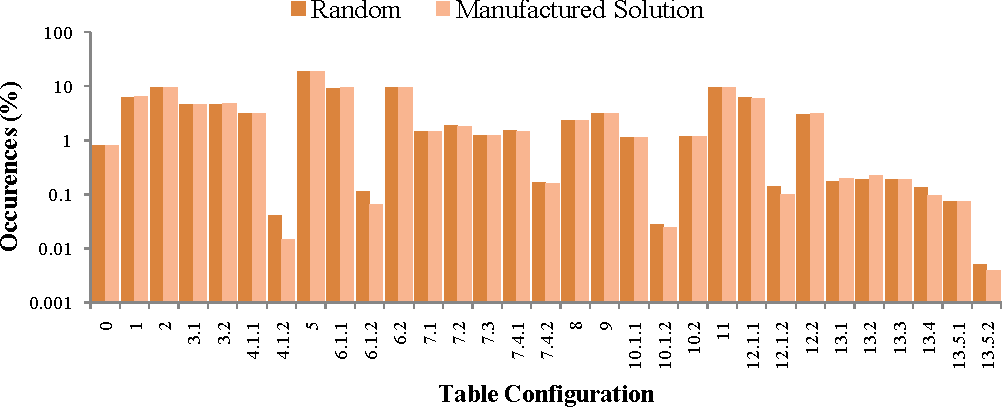
\includegraphics[width=1.0\linewidth,keepaspectratio=true]
{chapter3/figures/random-sampling.pdf}
\caption{The horizontal axis shows the case and subcase numbers for
  each of the 31 Marching Cubes configurations described by Lopes and
  Brodlie~\cite{lopes:tvcg:2003}. The dark bars show the percentage of
  random fields that fit a particular configuration. The light bars
  show the percentage of random fields which fit a particular
  configuration \emph{and} do not violate the assumptions of our
  manufactured solution.  Our manufactured solution hits all possible
  cube configurations.}
\label{fig:cubes-entries}
\end{figure}


% \begin{figure}
% \centering
% \includegraphics[width=0.7\linewidth,keepaspectratio=true]
% {chapter3/figures/mc33-case-00.pdf}
% \caption{An instance of one of the problems uncovered by our framework. From
% left to right: the output from $\proc{MarchingCubes33}$, the expected ouput
% \cite{Lewiner:2003} and the level-set beign extrated. A code mistake prevented
% the extraction of the right configuration.}
% \label{fig:mc33-problem}
% \end{figure}


Table \ref{tbl:verification-ds-stm} shows statistics for all 
implementations. For 
\mclewiner, the tests revealed a problem with configuration 4, 6, and 13 of
the table (ambiguous cases). Figure \ref{fig:problem-mclewiner} shows the
obtained and expected tiles for a cube. 
Contacting the author,
we found that one of the mismatches was due
to a mistake when coding configuration 13 of the MC table. A
non-obvious algorithm detail that is not
discussed in either Chernyaev's or Lewiner's work is the problem of orientation in
some of the cube configurations~\cite{Lewiner:2010:PC}. The case 13.5.2 shown in Figure
\ref{fig:problem-mclewiner} (right) is an example of one such configuration, where
an additional criterion is required to decide the tunnel orientation that is
lacking in the original implementation of \mclewiner. This problem was easily
detected by our framework, because the orientation changes the mesh
invariants, and a mismatch occurs.

\deliso\ presented a high percentage of $\beta_0$ mismatches due to the
mechanism used for tracking connected components. It uses ray-surface intersection to
sample a few points over each connected component of the isosurface before extracting it.
The number of rays is a user-controlled parameter and its initial position
and direction are randomly assigned. \deliso\ is likely to extract the biggest
connected component and, occasionally, it misses small components. It is
important to say that
the ray-sample based scheme tends to work fine in practical applications where
small
surfaces are not present. The invariant mismatches for $\beta_1$ and $\beta_2$
are computed only
if no consistency mismatch happens.

For \mcsimpleflow, we applied the verification
framework systematically during its implementation/development. Obviously, many
bugs were uncovered and fixed over the course of its development. 
%Noticie that this amount of tests is feasable only  using an
%automatic pipeline.
Since we are randomizing the piecewise trilinear field, we are
likely to cover all possible Marching Cubes entries and also different
cube combinations. As verification tests have been applied since the very beginning,
all detectable bugs were removed, resulting in no mismatches. 
The downside of \mcsimpleflow, though, is that typical bad quality
triangles appearing in Marching Cubes become even worse in
\mcsimpleflow,
because cubes of different sizes are glued together. 
\mcsimpleflow\ geometrical
convergence is presented in the supplementary material
\cite{scheidegger:techreport:2010}.

% We finish this section remebering that all three codes \mclewiner, \deliso\
% and \mcsimpleflow\ are still under development and constantly improving. 

\begin{figure}[t]
\centering
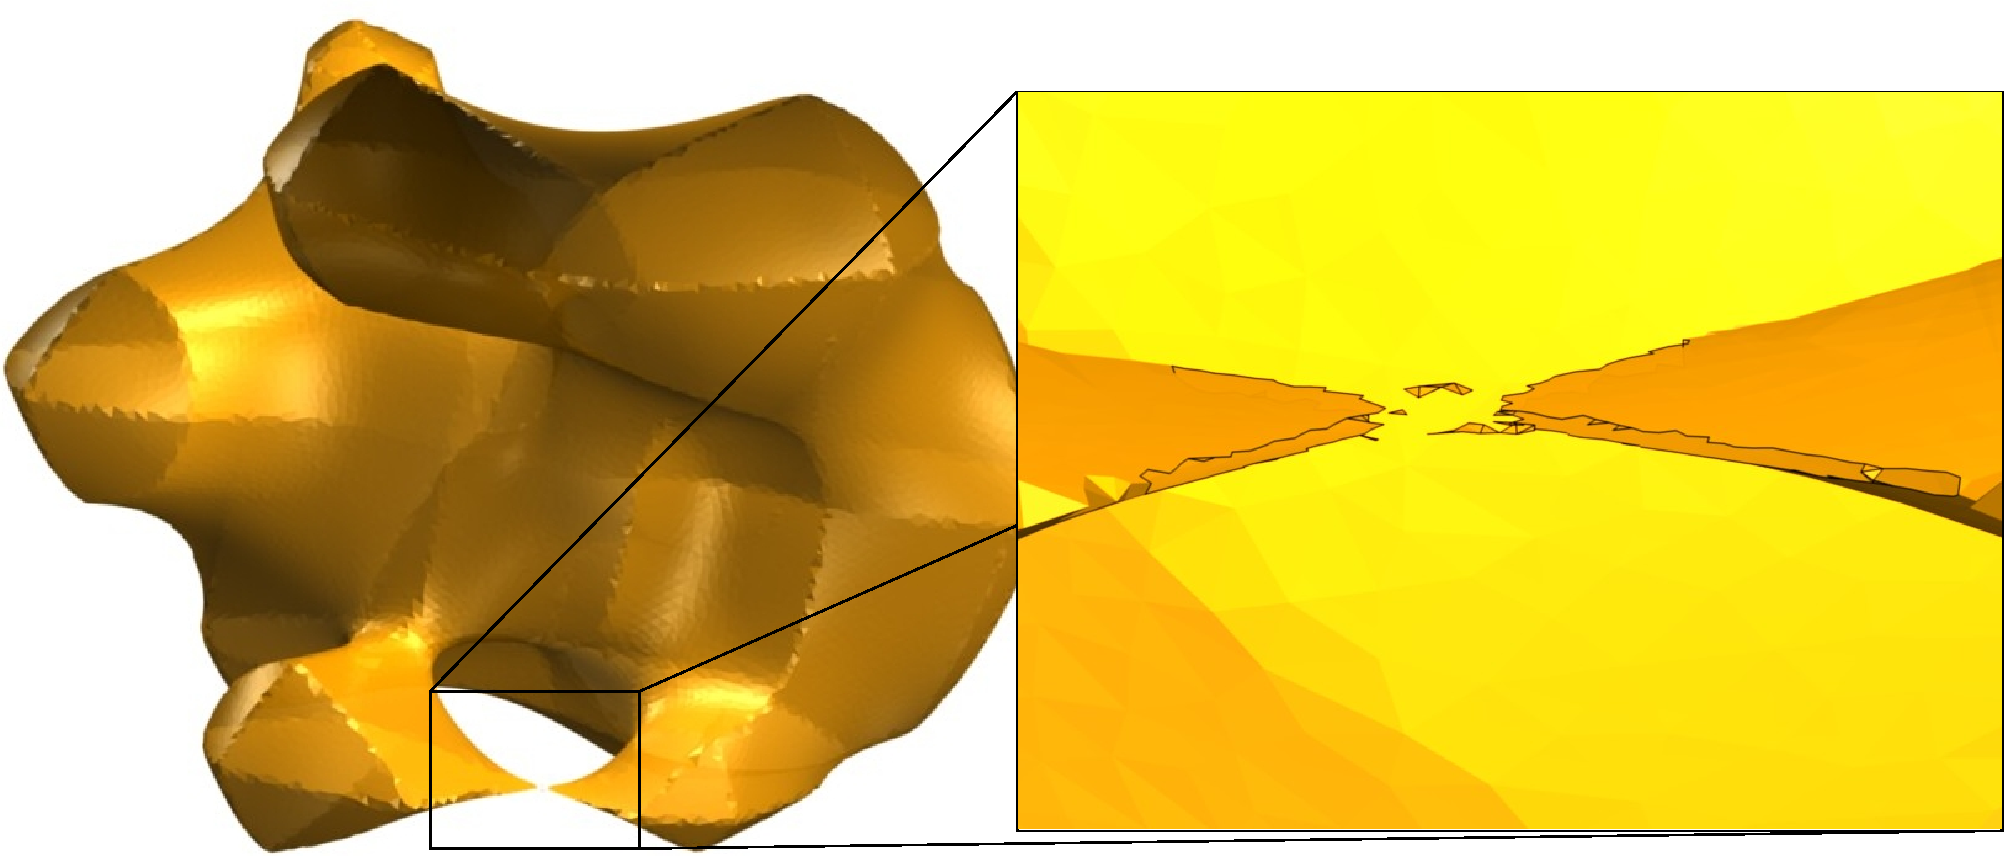
\includegraphics[width=0.33\linewidth,keepaspectratio=true]
{chapter3/figures/deliso-case-00.pdf}
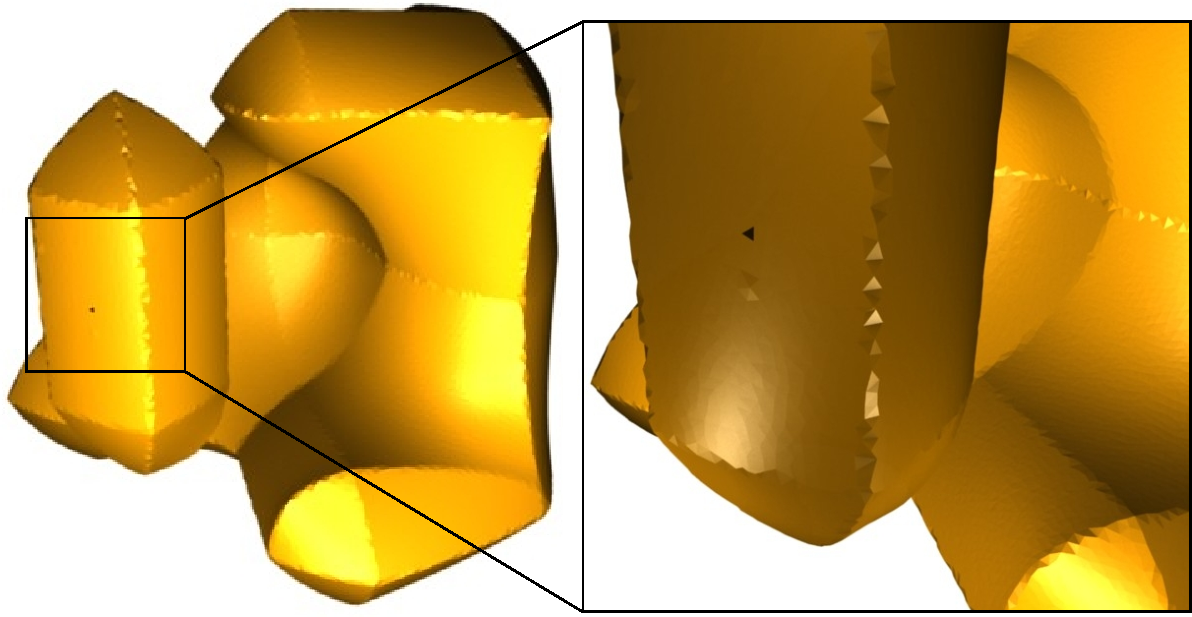
\includegraphics[width=0.3\linewidth,keepaspectratio=true]
{chapter3/figures/deliso-case-02.pdf}
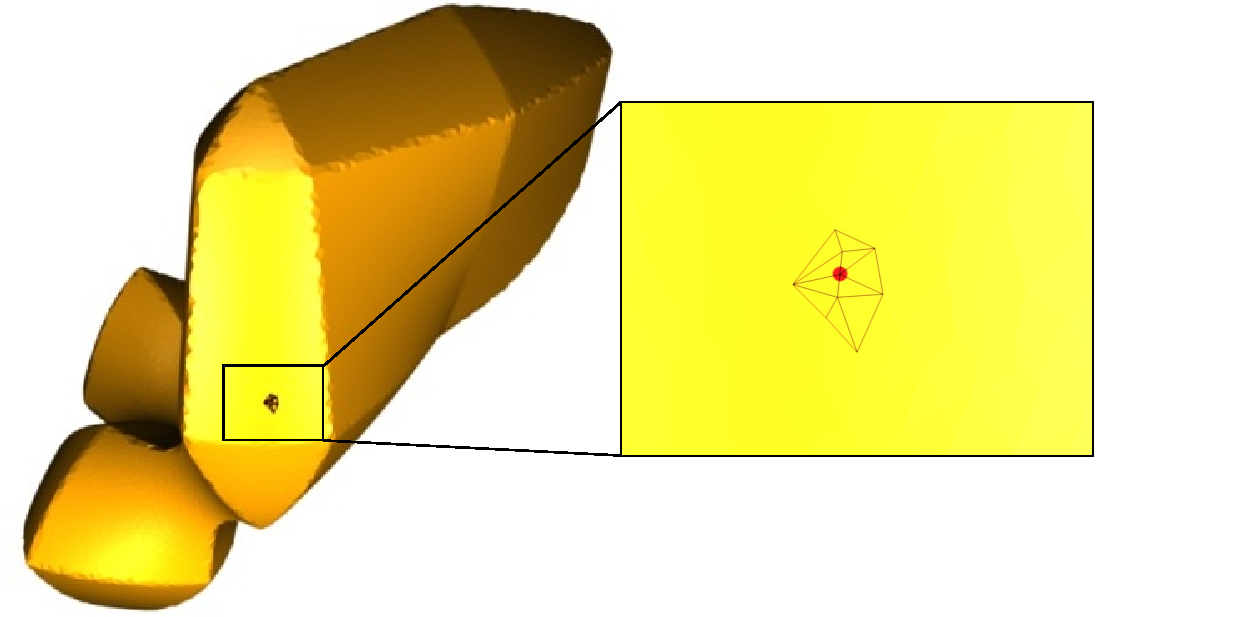
\includegraphics[width=0.29\linewidth,keepaspectratio=true]
{chapter3/figures/deliso-case-03.pdf}
\caption{\deliso\ mismatch example. From left to right: holes in $C^0$
  regions; single missing triangle in a smooth region; duplicated
  vertex (the mesh around the duplicated vertex is shown). These
  behavior induce topology mismatches between the generated mesh and
  the expected topology.}
\label{fig:pproblem-deliso}
\end{figure}

\begin{figure}[t]
\centering
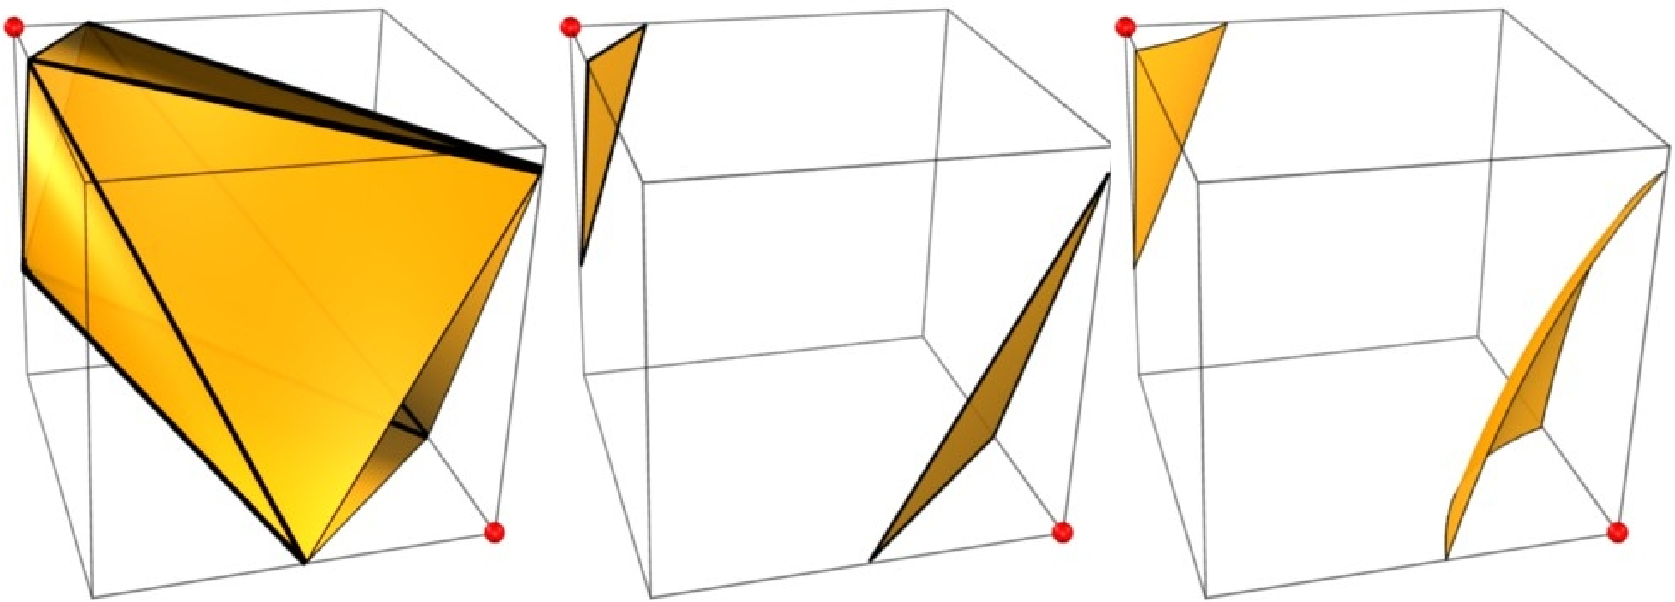
\includegraphics[width=0.3\linewidth,keepaspectratio=true]
{chapter3/figures/mc33-case-02.pdf} ~~~~
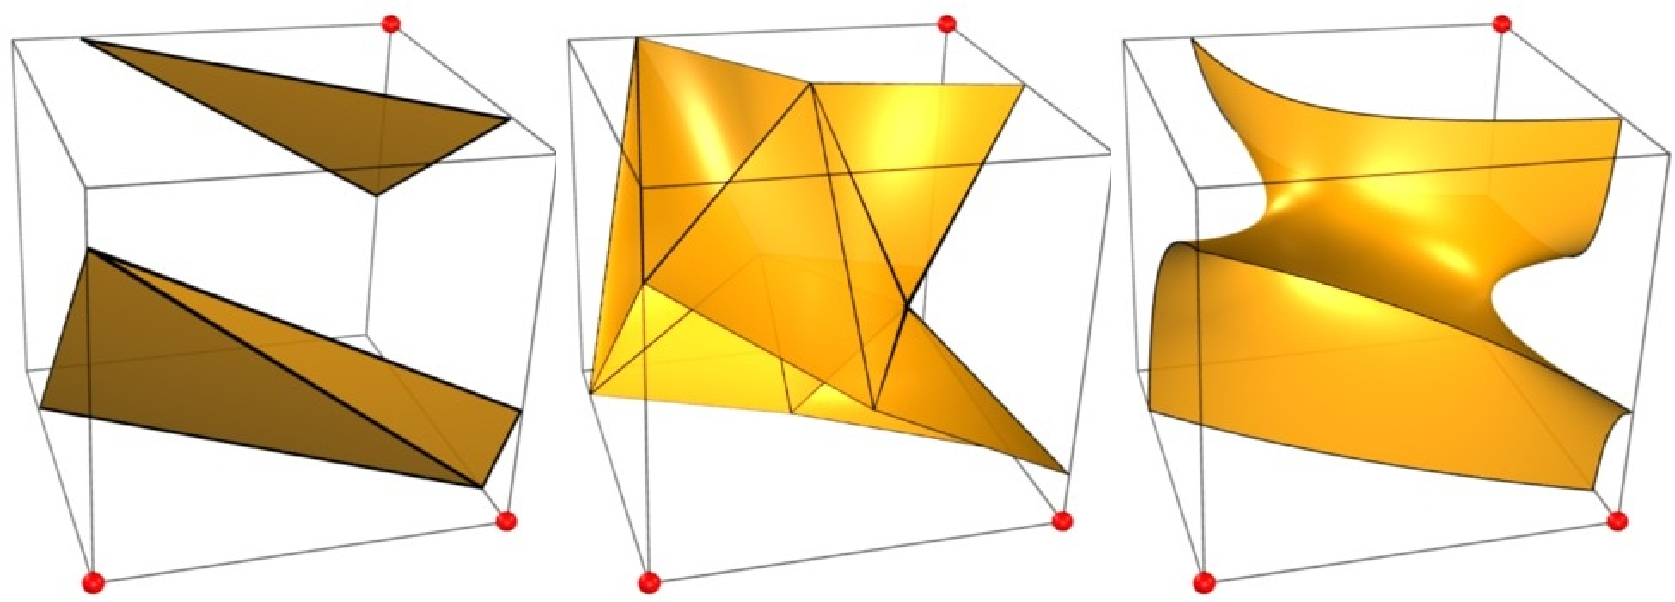
\includegraphics[width=0.3\linewidth,keepaspectratio=true]
{chapter3/figures/mc33-case-01.pdf} ~~~~
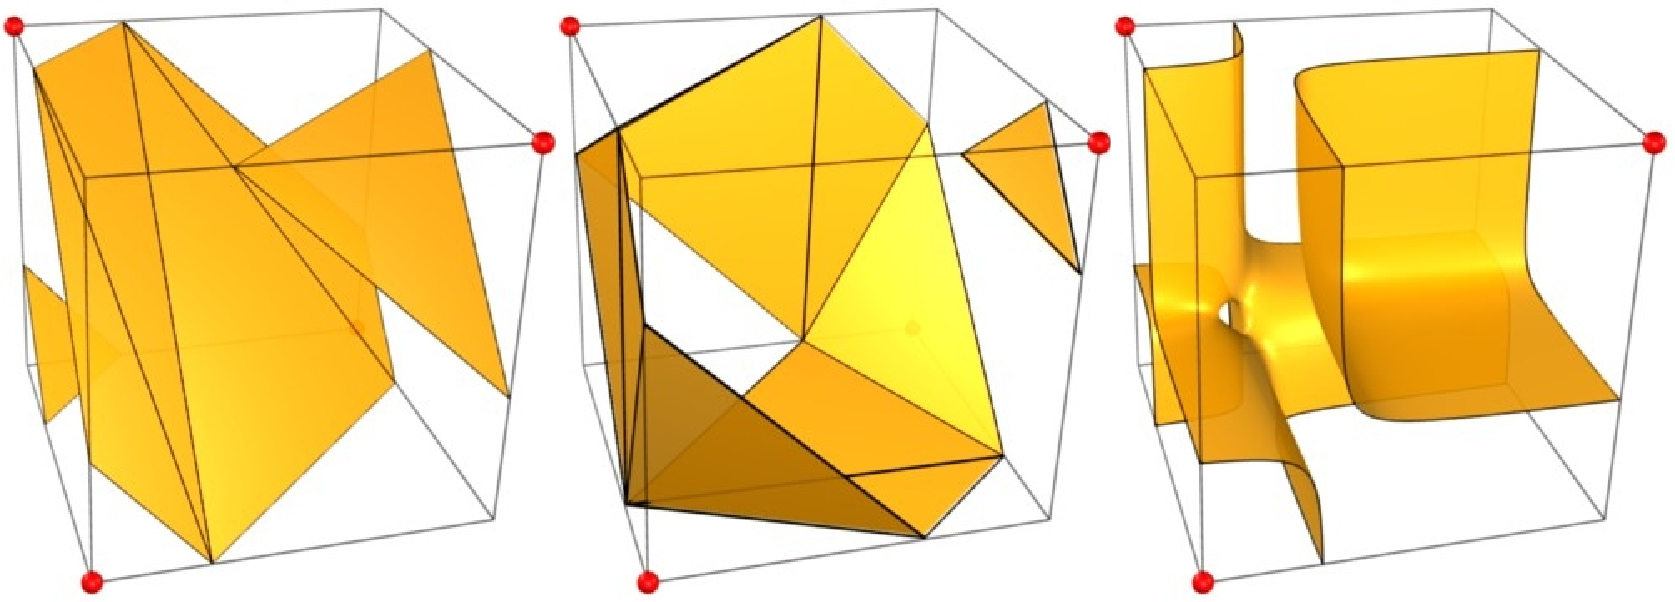
\includegraphics[width=0.3\linewidth,keepaspectratio=true]
{chapter3/figures/mc33-case-00.pdf} 
\caption{\mclewiner\ mismatch example. From left to right: problem in
  the case 4.1.2, 6.1.2, and 13.5.2 of marching cube table (all are
  ambiguous). Each group of three pictures shows the obtained,
  expected, and implicit surfaces. Our verification procedure can
  detect the topological differences between the obtained and expected
  topologies, even for ambiguous cases.}
\label{fig:problem-mclewiner}
\end{figure}


\begin{figure}[t]
\centering
\subfigure[\snapmc\ (0.3)]{
\label{fig:inconsistencies:snapmc}
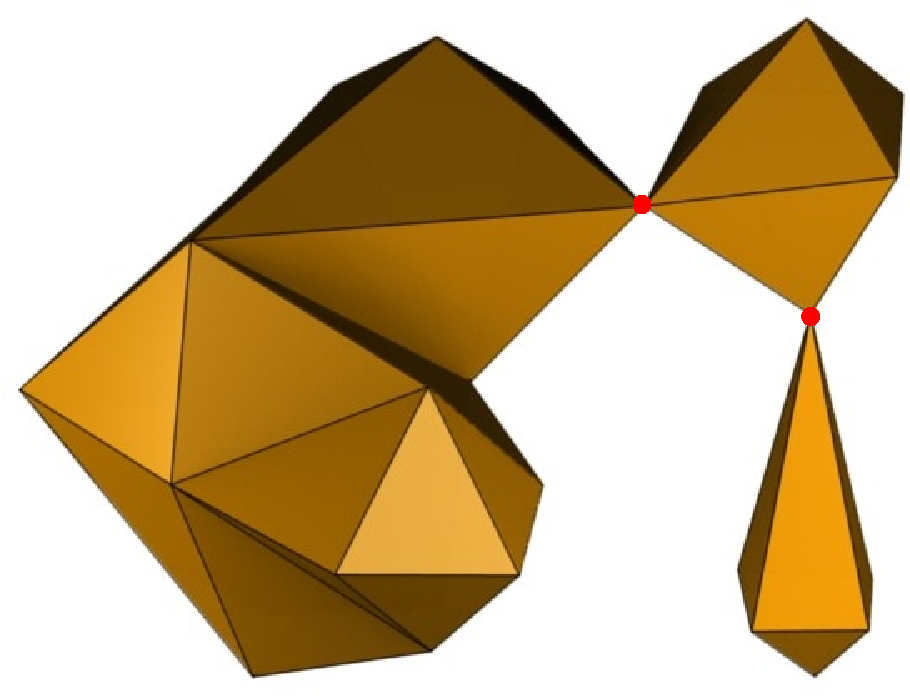
\includegraphics[width=0.20\linewidth,keepaspectratio=true]
{chapter3/figures/snapmc_00.pdf}} ~~~~~~~~
\subfigure[\matlab]{
\label{fig:inconsistencies:matlab}
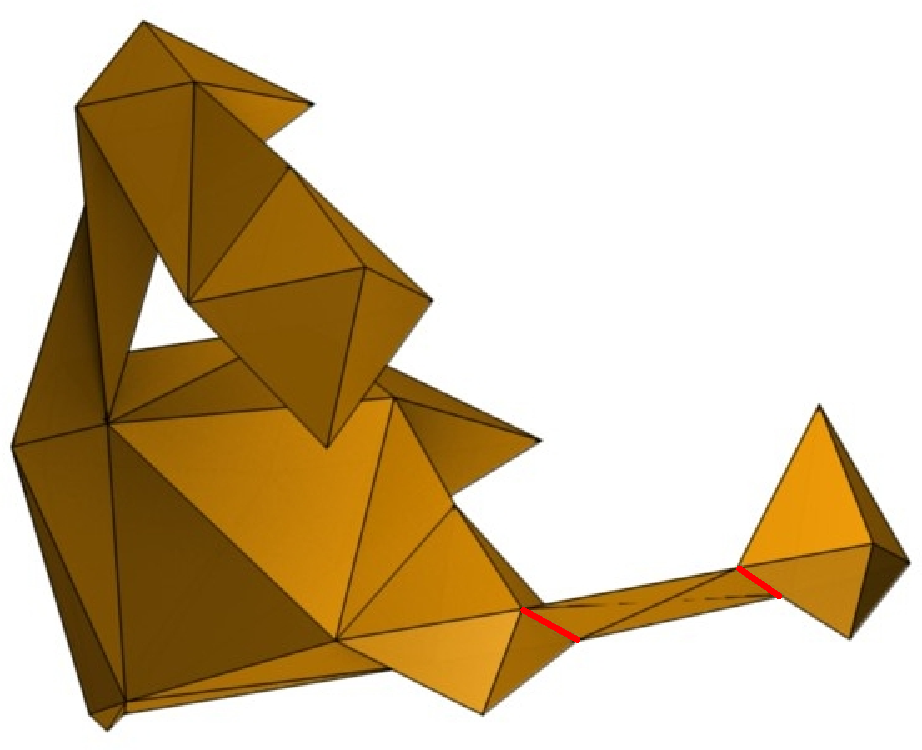
\includegraphics[width=0.20\linewidth,keepaspectratio=true]
{chapter3/figures/matlab_00.pdf}} ~~~~~~~~
\subfigure[\mcsimpleflow]{
\label{fig:problem-mcsimpleflow}
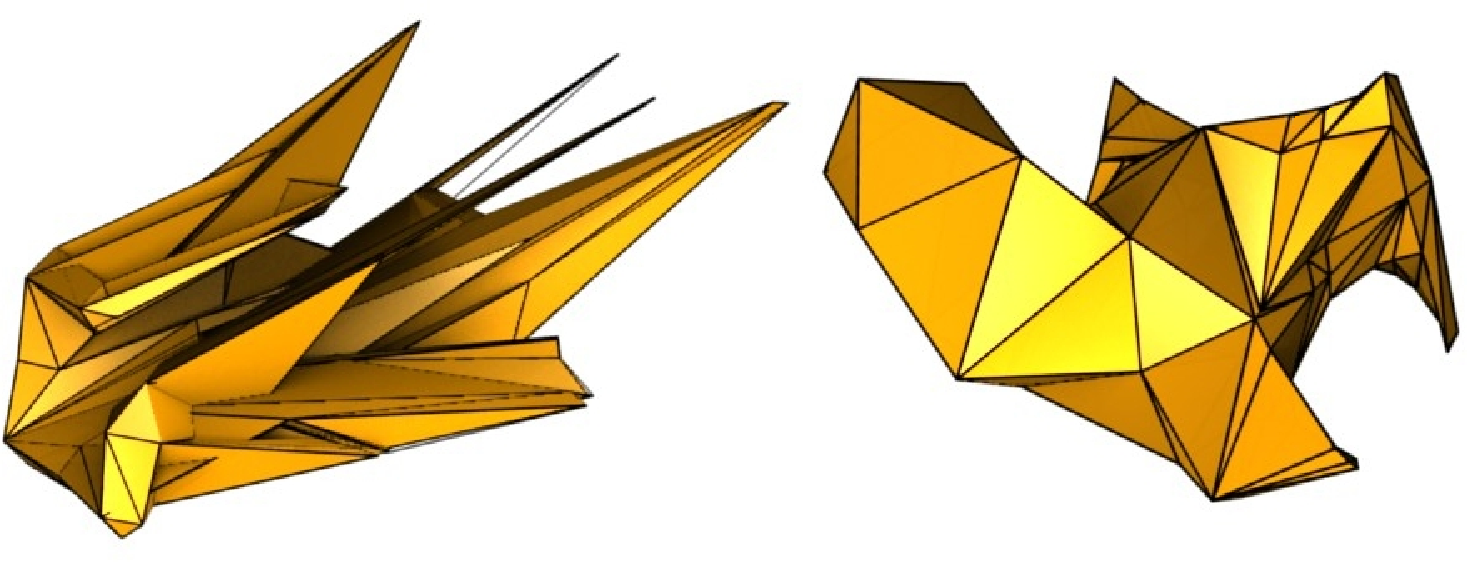
\includegraphics[width=0.37\linewidth,keepaspectratio=true]
{chapter3/figures/our_mc.pdf}}
\caption{Mismatches in topology and geometry. (a) \snapmc\ generates
  non-manifold surfaces due to the snap process. (b)
  \matlab\ generates some edges (red) that are shared by more than two
  face. (c) \mcsimpleflow before (left) and after (right) fixing a bug
  that causes the code to produce the expected topology, but the wrong
  geometry.}
\label{fig:inconsistencies}
\end{figure}


\section{Discussion and Limitations}
\label{sec:discussion}

\subsection{Quality of manufactured solutions}
In any use of MMS, one very important question is that of the quality
of the manufactured solutions, since it reflects directly on the
quality of the verification process. Using random solutions, for which
we compute the necessary invariants, naturally seems to yield good
results. However, our random solutions will almost always have
nonidentical values. This raises the issue of detecting and handling
degenerate inputs, such as the ones arising from quantization. We
note that most implementations use techniques such as Simulation of
Simplicity~\cite{Edelsbrunner:1990:SOS} (for example, by arbitrarily breaking ties using node
ordering) to effectively keep the facade of nondegeneracy. However, we note
that developing manufactured solutions
specifically to stress degeneracies is desirable when using
verification tools during development. We decided against this since
different implementations might employ different strategies to handle
degeneracies and our goal was to keep the presentation sufficiently
uniform.

\begin{table}[b]
\caption{Rate of invariant mismatches using the PL manifold property, digital
surfaces, and stratified Morse theory for $1000$ randomly generated
scalar fields (the lower the rate the better).
The invariants $\beta_1$ and $\beta_2$ are computed only if the output mesh is a
2-manifold without boundary. \emph{We run correctness tests in all algorithms for
completeness and to test tightness of the theory: algorithms that are not
topology-preserving should fail these tests}. 
The high number of \deliso, \snapmc, and \matlab\ mismatches are explained in
Section \ref{sec:consistency}. 
$^1$ indicates zero snap parameter and $^2$ indicates snap value of
0.3.}
\begin{center}
\begin{tabular}{l@{}cccccc}
   & Consistency (\%) &\multicolumn{5}{c}{Correctness (\%)} \\
\hline
    &\multirow{2}{*}{Disk} &\multicolumn{4}{c}{Digital Surfaces} &
SMT\\
              &        &$\beta_0$ & $\beta_1 $ & $\beta_2 $ & $\chi$ & $\chi$ \\
\hline
\afront       & ~$0.0$  & $35.9$  & $22.8$ & $35.9$ & $47.5$ & ~$25.5$
\\
\Matlab       & $19.7$  & $32.2$  & $18.9$ & $20.5$ & $49.3$ & ~$70.3$
\\
\vtk          & ~$0.0$  & $27.6$  & $23.2$ & $27.6$ & $43.5$ & ~$70.7$
\\
\hline
\macet        & ~$0.0$  & $54.3$  & $20.9$ & $54.3$ & $64.0$ & $100.0$
\\
\snapmc$^1$   & ~$0.0$  & $45.0$  & $25.4$ & $45.0$ & $57.3$ & ~$72.0$
\\
\snapmc$^2$   & $53.7$  & $41.6$  & $17.3$ & $23.1$ & $87.1$ & ~$74.0$
\\
\hline
\mclewiner    & ~$0.0$  & ~$2.4 $ & ~$1.1$ & ~$2.4$ & ~$3.4$ & ~~$5.4$ 
\\
\deliso       & $19.1$  & $24.4$  & ~$0.1$ & $20.0$ & $37.2$ & ~$33.2$ 
\\
\mcsimpleflow & ~$0.0$  & ~$0.0$  & ~$0.0$ & ~$0.0$ & ~$0.0$ & ~~$0.0$ 
\\
\hline
\end{tabular}
\label{tbl:verification-ds-stm}
\end{center}
\end{table}


\subsection{Topology and Geometry}
This work extends the work by Etiene et al.~\cite{etiene:tvcg:2009} toward
including topology in the loop of verification for isosurface techniques. 
The machinery presented herein combined with the methodology for verifying
geometry comprises a solid battery of tests able to stress most of the existing 
isosurface extraction codes. 

To illustrate this, we also submitted \mclewiner\ and \mcsimpleflow\ techniques 
to the geometrical test proposed by Etiene, as these codes have not been 
geometrically verified. While \mclewiner\ has geometrical
behavior in agreement with Etiene's approach, the results presented in Section~\ref{sec:results} 
show it does not pass the topological tests. 
%our framework revealed a code mistake. 
On the other hand, after ensuring that 
\mcsimpleflow\ was successful regarding topological tests, 
we submitted it to the geometrical analysis, which revealed problems.
Figure \ref{fig:problem-mcsimpleflow} shows an
example of an output generated in the early stages of development of \mcsimpleflow\ before (left) and after
(right) fixing the bug. The topology matches the expected one (a
topological sphere); nevertheless, the geometry does not converge. 


% \paragraph*{Interpreting behavior}
% We have talked to the authors of two of the techniques under verification to
% understand the behavior shown in Table \ref{tbl:verification-ds-stm}. As
% explained earlier, \mclewiner\ had a code mistake that prevent it from
% generate
% the right topology for configuration 13.5.2 of Marching Cubes table. Even
% after
% fixing it, there were still some mismatches that need to be explained which
% motivates the verification cycle. 
% \paragraph*{Topology Consistency vs. Correctness}

\subsection{SMT vs. DT}
The verification approach using digital surfaces generates detailed
information about the expected topology because it provides $\beta_0$, $\beta_1$, and $\beta_2$. 
However, verifying isosurfaces with boundaries would require
additional theoretical results, as the theory supporting our verification
algorithm is only valid for surfaces without boundary.
%The current framework does not deal with surfaces touching the
%boundary of the domain although it can be extended to account for it. 
In contrast, the verification methodology using stratified Morse theory can handle
surfaces with boundary. However, SMT only provides information 
about the Euler characteristic, making it harder to determine when the topological verification process fails.
%Since many application requires extraction of isosurfaces with boundaries, it is
%also important they are computed correctly. 
Another issue with SMT is that if a code incorrectly introduces topological features so as
to preserve $\chi$, then no failure will be detected. For example, suppose the surface to
be reconstructed is a torus, but the code produces a torus plus three triangles,
each one sharing two vertices with the other triangles but not an edge. In this case, 
torus plus three ``cycling'' triangles also has $\chi = 0$, exactly the Euler characteristic of the single torus.
In that case, notice that the digital surface-based test would be able to
detect the spurious three triangles by comparing $\beta_0$.
Despite being less sensitive in theory, 
SMT-based verification revealed similar problems as the digital topology tests have. 
We believe this effectiveness comes in part from 
the randomized nature of our tests.

\subsection{Implementation of SMT and DT}
Verification tools should be as simple as possible while still
revealing unexpected behavior. The pipeline for geometric
convergence is straightforward and thus much less error-prone. This is
mostly because
Etiene et al.'s approach uses analytical manufactured solutions to provide
information about function value, gradients, area, and curvature. In topology,
on the other hand, we can manufacture only simple analytical solutions (e.g., a
sphere, torus, double-torus, etc.) for which we know topological
invariants. There are no guarantees that these solutions will cover all
cases of a trilinear interpolant inside a cube. For this reason, we
employ a random manufactured solution and must then compute
explicitly the topological invariants.
A point which naturally arises in verification settings is that the verification code is another program. 
How do we verify the verifier?

First, note that the implementation of either verifier is simpler than
the isosurfacing techniques under scrutiny. This reduces the chances
of a bug impacting the original verification.  In addition, we can use
the same strategy to check if the verification tools are implemented
correctly. For SMT, one may compute $\chi$ for an isovalue that is
greater than any other in the grid. In such case, the verification
tool should result in $\chi = 0$. For DT, we can use the fact that
Majority Interpolation always produces a 2-manifold. Fortunately, this
test reduces to check for two invalid cube configurations as described
by Stelldinger et al.~\cite{siqueira:2007}. Obviously, there might
remain bugs in the verification code. As we have stated before, a
mismatch between the expected invariants and the computed ones
indicates a problem \emph{somewhere} in the pipeline; our experiments
are empirical evidence of the technique's effectiveness in detecting
implementation problems.

Another concern is the performance of the verification tools. In our
experiments, the invariant computation via SMT and DS is faster than
any isosurface extraction presented in this work, for most of the
random grids. In some scenarios, DS might experience a slowdown
because it refines the grid in order to eliminate ambiguous cubes (the
maximum number of refinement is set to 4). Thus, both SMT and DS (after
grid refinement) need to perform a constant number of operations
for each grid cube to determine the digital surface (DS) or critical
points (SMT).  In this particular context, we highlight the recent
developments on certifying algorithms, which produce both the
output and an \emph{efficiently checkable certificate of
  correctness}\cite{McConnell:2010:CA}.


\subsection{Contour Trees}
Contour trees \cite{Hamish03} are powerful structures to describe the
evolution of level-sets of simply connected domains. It normally
assumes a simplicial complex as input, but there are extensions to
handle regular grids\cite{Pascucci03}. Contour trees naturally provide
$\beta_0$, and they can be extended to report $\beta_1$ and
$\beta_2$. Hence, for any isovalue, we have information about all
Betti numbers, even for surfaces with boundaries.  This fact renders
contour trees a good candidate for verification purposes. In fact, if an
implementation is available, we encourage its use so as to increase
confidence in the algorithm's behavior.  However, the implementation of
a contour tree is more complicated than the techniques presented here.
For regular-grids, a divide-and-conquer approach can be used along
with oracles representing the split and join trees in the deepest
level of the recursion, which is non-trivial. Also, implementing the
merging of the two trees to obtain the final contour tree is still
involving and error-prone.  Our approach, on the other
hand, is based on regular grid refinement and voxel selection for the DT
method and critical point computation and classification for the SMT
method.  There are other tools, including contour trees, that could be
used to assess topology correctness of isosurface extraction
algorithms, and an interesting experiment would be to compare the
number of mismatches found by each of these tools.  Nevertheless, in
this work, we have focused on the approaches using SMT and DT because
of their simplicity and effectiveness in finding code
mistakes in publicly available implementations.  We believe that the
simpler methodologies we have presented here are more likely to be
adopted during development of visualization isosurfacing tools.

\subsection{Topology of the underlying object}
In this work, we are interested in how to effectively verify
topological properties of codes which employ trilinear
interpolation. In particular, this means that our verification tools
will work for implementations other than marching methods (for
example, DelIso is based on Delaunay refinement).
%
Nevertheless, in practice, the original scalar field will not be
trilinear, and algorithms which assume a trilinearly interpolated
scalar field might not provide any topological guarantee regarding the
reconstructed object.
%scientists may be interested in the topology of the \emph{original
%object} instead of a trilinear interpolant. 
Consider, for example, a piecewise linear curve $\gamma$ built by
walking through diagonals of adjacent cubes $c_i \in \mathcal{G}$ and
define the distance field $d(x) = \min\{||x - x'||\, \text{such
  that}\ x'\in\gamma\}$. The isosurface $d(x) = \alpha$ for any
$\alpha > 0$ is a single tube around $\gamma$.  However, none of the
implementations tested could successfully reproduce the tubular
structure for all $\alpha > 0$. This is not particularly surprising,
since the trilinear interpolation from samples of $d$ is quite
different from the $d$.
\begin{wrapfigure}{l}{4.5cm}
\vspace{-0.2cm}
\hspace{-0.0cm}
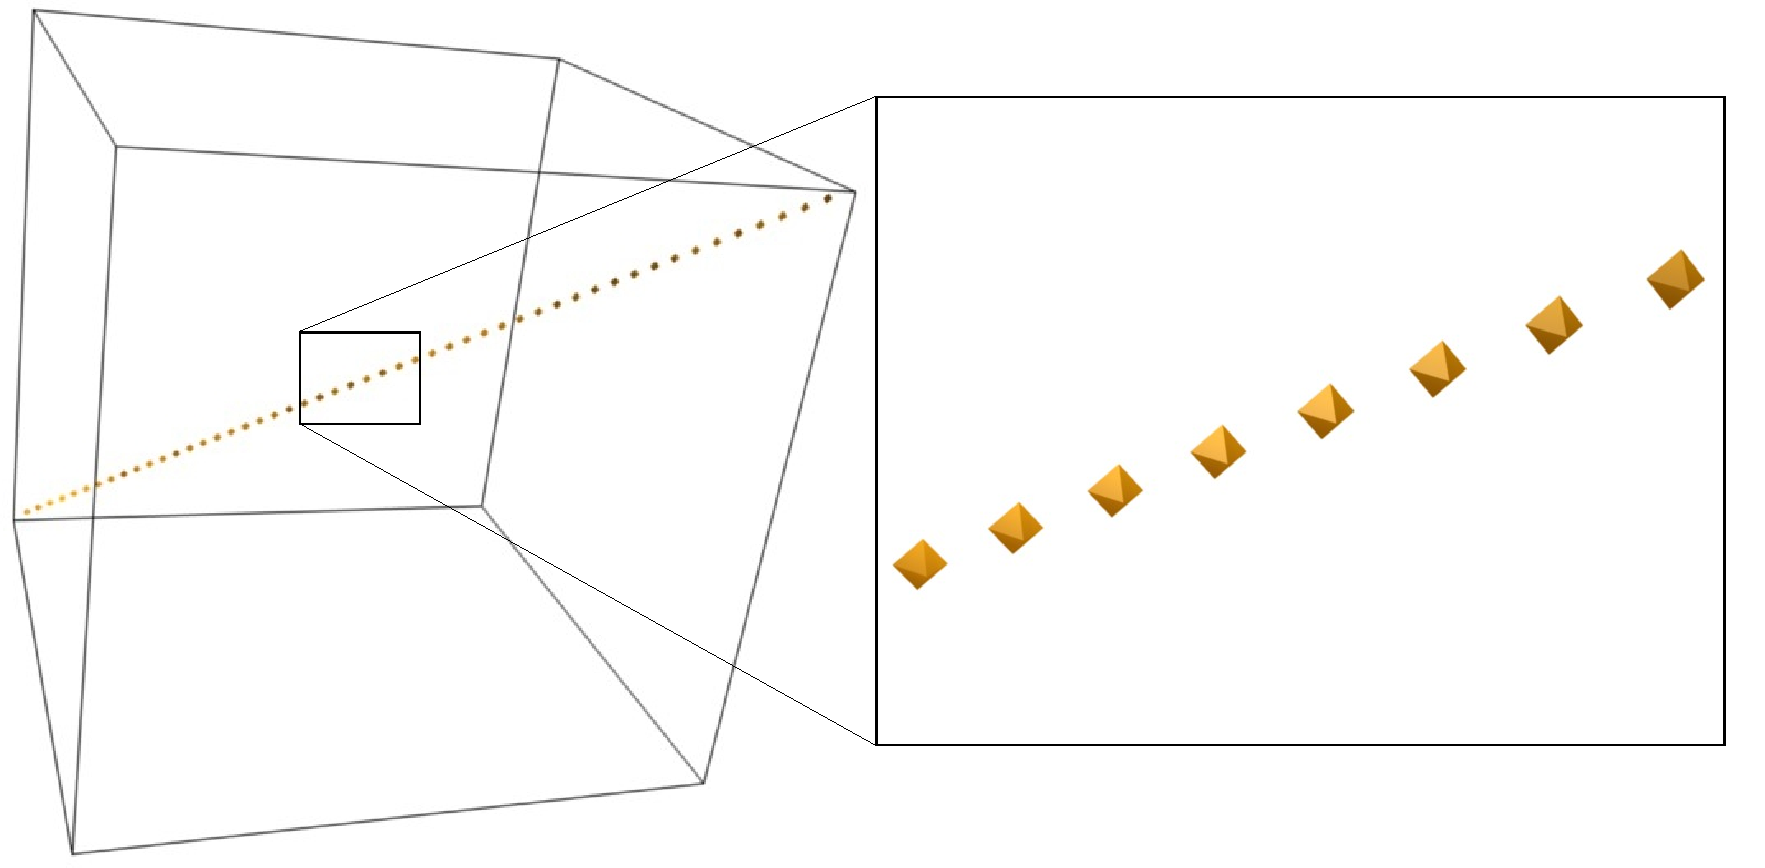
\includegraphics[width=0.7\linewidth,keepaspectratio=true]
{chapter3/figures/distance-field.pdf}
\end{wrapfigure}
The inline figure on the right shows a typical output produced by VTK
Marching Cubes for the distance field $d = \alpha$. Notice, however,
that this is not only an issue of sampling rate because if the tube
keeps going through the diagonals of cubic cells, VTK will not be able
reproduce $d = \alpha$ yet.  Also recall that some structures cannot
even be reproduced by trilinear interpolants, as when
$\gamma$ crosses diagonals of two parallel faces of a cubic cell, as
described in \cite{Chernyaev95marchingcubes, Pascucci03}.  The aspects
above are not errors in the codes but reflect software design choices
that should be clearly expressed to users of those visualization
techniques.

%Other interpolants could be used to reconstructu guiding the meshing
%template in each cube considering that this is an issue related to
%the disambiguation scheme employed and not necessarily a code
%mistake.  In the scenario described above, the isovalue can be
%changed slightly or the disambiguation scheme could be altered in
%order to reproduce the tubes correctly but some curves crossing
%cannot even be reproduced by trilinear interpolant Any interpolant
%can be used to approximate the topology of the original
%object. However, there are only a handful of cases were one can
%guarantee that the extracted surface is homeomeorphic to the
%underlying object.

\subsection{Limitations}
The theoretical guarantees supporting our manufactured solution
rely on the trilinear interpolant.  
If an interpolant other than trilinear is employed, then new results ensuring
homeomorphism (Theorem 4.1) should be derived. 
The basic infrastructure we have described here, however,
should be appropriate as a starting point for the process.


\section{Conclusion and Future Work}

We extended the framework presented by Etiene et al.
\cite{etiene:tvcg:2009} by including topology into the verification
cycle.  We used machinery from digital topology and stratified Morse
theory to derive two verification tools that are simple and yet
capable of finding unexpected behavior and coding mistakes.
%
We argue that researchers and developers should consider adopting
verification as an integral part of the investigation and development
of scientific visualization techniques.  Topological properties are as
important as geometric ones, and they deserve the same amount of
attention. It is telling that the only algorithm that passed all
verification tests proposed here is the one that used
the verification procedures \emph{during} its development. We believe
this happened because topological properties are particularly subtle
and require an unusually large amount of care.

The idea of verification through manufactured solutions is clearly problem-dependent
and mathematical tools must be tailored accordingly. 
Still, we expect the framework to enjoy a similar effectiveness in many areas of scientific visualization,
including volume rendering, streamline computation, and mesh simplification.
%Those areas have been extensively studied and would likely benefit from a verification
%framework.
We hope that the results of this work further motivate the visualization
community to develop a culture of verification.

%We should highlight that this is just a brick to the new field of
%verification for visualization.  This is a valuable tool for
%verification. There are several ways to extend this: volume
%rendering, streamlines, simplification, etc.  All these algorithms
%are part of critical pipelines and thus its correctness is of great
%importance. (We have to polish this)

%We should include some complexity analysis (although it doesn't
%matter). It will be easy and the reviewers will be happy.  Bullet
%points contribuitions. We should emphasize this whole new field of
%verification in the introduction. We should emphasize that this has
%not been done before. Similar work, like Edelbrunner, doesn't cover
%this.

%% if specified like this the section will be ommitted in review mode
\section*{Acknowledgments}
We thank Thomas Lewiner and Joshua Levine for
  help with \mclewiner\ and \deliso\ codes respectively.
This work was supported in part by grants from
%  the National Science Foundation
  NSF
 (grants IIS-0905385, IIS-0844546,
  ATM-0835821, CNS-0751152, OCE-0424602, CNS-0514485, IIS-0513692,
  CNS-0524096, CCF-0401498, OISE-0405402, CCF-0528201, CNS-0551724,
  CMMI 1053077, IIP 0810023, CCF 0429477),
  DOE,
%  the Department of Energy, 
  IBM Faculty Awards and PhD Fellowship, the
  US ARO % Army Research Office
  under grant W911NF0810517, ExxonMobil, and
  Fapesp-Brazil (\#2008/03349-6).


\chapter{Practical Considerations on the Topological Correctness of Marching Cubes 33}
\label{chap:mc33}

Isosurface extraction techniques can be divided into two classes according to their topological guarantees, namely, consistency or correctness. Topologically \emph{consistent} techniques produce surfaces that are piecewise-linear (PL) manifolds (\emph{i.e.}, crack-free surfaces), except at the boundary of the domain. To-pologically \emph{correct} techniques produce a PL-manifold homeomorphic to the surface induced by a given interpolant, such as the trilinear interpolant. Although there are many topologically \emph{consistent} MC-based techniques, only a handful are topologically \emph{correct}. Marching Cubes 33 is one of the first MC-based algorithms that aim to preserve the topology of the trilinear interpolant.

Topological correctness increases the complexity of isosurface extraction algorithms. 
The many isosurface configurations possible for a given interpolant in a cubic grid makes both the algorithm and its implementation a challenging task. 
%
As algorithms and implementations become more complex, issues may be overlooked and remain hidden in the multitude of (pseudo-) lines of code.
%
Throughout years of research, it has been shown that some supposedly topologically correct techniques, including \mc, have issues that prevent correctness  \cite{Etiene:2012:TVI:2197070.2197097, lopes:tvcg:2003, newman:candg:2006}. 
%
In particular, the work of Etiene \emph{et al.} \cite{Etiene:2012:TVI:2197070.2197097} shows that the \mc{} implementation by Lewiner \emph{et al.} \cite{lewiner:impl,Lewiner:2003}, fails to produce topologically correct isosurfaces. 
%
Alas, the authors \emph{do not} provide an explanation for the problem source, let alone fix the problem. 
%
They only provide cases that are mishandled by \mc{} and a conjecture regarding  the root of one of the observed flaws.
%
As we studied the \mc{} implementation, we realized that the source of the problem was not merely implementation bugs but the core ideas behind the implemented algorithm.  
%
In this work, we address issues with Chernyaev's original algorithm, its extension, and its implementation. 
%
Our work closes an existing gap in the topological correctness of Marching Cubes 33.
 
 The subtleties involved in the correctness of isosurface extraction techniques are sometimes difficult to grasp in the ordinary paper medium. Both the geometry and topology inside grid voxels are often complex and challenging to understand,  study and replicate ({\em e.g.}, see Figures 9 and 10 in~\cite{Nielson03onmarching}).  As an attempt to bridge this gap, we build on recent efforts towards \emph{executable papers}~\cite{Koop:2011tv, Tohline:2010jn}. Executable papers extend the traditional paper/digital counterpart by including tools that allow readers to interact, explore and verify experiments more easily.  In this chapter, we use executable papers to increase the reproducibility of our results.
 %
 
Our contributions, which have a practical nature, are the following:
\begin{itemize}
\item We explain and address three algorithmic issues and one non-trivial implementation issue with Marching Cubes 33. In particular, we solve an issue with the core \mc{} disambiguation procedure that, as far as we know, has not been addressed elsewhere. Hence, we close an existing gap in the \mc{} literature.
\item We make our results reproducible. CrowdLabs~\cite{Tohline:2010jn} and Vistrails \cite{Freire:2006va} are used to create an executable paper that can reproduce the results shown in the following sections.
\item We provide datasets that  can be used to verify the correctness of any topologically correct isosurface extraction technique.
\end{itemize}
A by-product of this work is a thorough analysis of both the \mc{} algorithm and its implementation that can be used by anyone interested in  the use or development of correct isosurface extraction algorithms based on \mc{}. The results of our efforts are materialized into an extended version of the \mc{} implementation \cite{lewiner:impl}, henceforth called Corrected-MC33 (\cmc).

This work is organized as follows. Section \ref{sec:preliminaries} reviews key aspects related to the Marching Cubes 33 algorithm. Section \ref{experiments_setup} explains how experiments that uncovered problems in both \mc{} algorithm and implementation were conducted. The details of the problems found are shown in Section \ref{erros_cause:chernyaev} and the solutions are presented in Section \ref{sec:solution}. Section \ref{sec:real-world} shows the results of applying algorithm with different topological guarantees to real-world datasets.

%============================================================================================



\section{Related Work}
\label{related_work1}

Soon after the publication of the MC algorithm, the quest for a topologically correct isosurface extraction technique began. A number of approaches were proposed for dealing with cracks, face ambiguity, and, lastly, interior ambiguity.
%
D\"urst \cite{Durst88} was the first to point out that some MC cases allow multiple triangulations. A consequence of this is that MC does not always generate topologically consistent surfaces. This problem arises due to the \emph{ambiguity problem}; and
the Asymptotic Decider \cite{Nielson:1991:ADR:949607.949621} provides a simple and elegant solution to face ambiguity.

The ambiguity problem also occurs in the interior of a voxel. Natarajan \cite{Natarajan:1994:GTC:205424.205429}  was the first to address this problem by adding four new cases to the standard MC triangulation table (subcases of cases 3, 4, 6, and 7). To find the correct subcases, the author proposed a disambiguation procedure based on both face and interior critical points. Nevertheless,  the method misses the possibility of two interior critical points in case 7, consequently the proposed algorithm may generate a surface with the incorrect topology~\cite{10.1109/TVCG.2009.10, newman:candg:2006}.

Using a different approach, Chernyaev \cite{Chernyaev95marchingcubes} extended the original MC table to 33 cases -- hence \mc{}; this extension included all the subcases for each ambiguous case. He used the Asymptotic Decider and a new interior ambiguity test to discriminate among subcases. Lewiner \emph{et al.} \cite{Lewiner:2003} provided a practical open-source implementation of the Chernyaev algorithm. It is worth noting that some of the configurations shown in Chernyaev's work~\cite{Chernyaev95marchingcubes} may have been inspired by personal communication with Nielson \cite{Nielson03onmarching}.
%
Matveyev~\cite{Matveyev99} introduced an isosurface technique that is also based on an extended table and used the intersections of isosurfaces with cube diagonals to determine the correct case. 

Lopes and Brodlie \cite{lopes:tvcg:2003} extended the tests proposed by Natarajan. The goals of the work are threefold: i) extract topologically correct isosurfaces; ii) produce geometrically accurate isosurface; iii) allow continuity with respect to changes in threshold and data.  Nevertheless, as in Natarajan's work, the method missed the possibility of two interior critical points in case 7~\cite{lopes:tvcg:2003}.
%
Cignoni \emph{et al.}~\cite{Cignoni2000399} also used the test proposed by Natarajan to reconstruct topologically correct isosurfaces.
%
The work of Theisel \cite{CGF:CGF00563} uses B\'ezier patches to build $G^1$ continuous isosurfaces that are topologically correct.  Nielson \cite{Nielson03onmarching} lists all possible cases of a trilinear interpolant inside a cubic grid and builds a topologically correct MC using a three stage algorithm for surface polygonization. 

The past two decades have also produced a number of isosurface techniques that are not MC-based. Dual Contouring~\cite{Ju:2002:DCH:566654.566586} (DC) is a robust, crack-free, isosurface extraction technique that works on the dual grid. Several improvements over Dual Contouring have been proposed: Schaefer \emph{et al.}~\cite{Schaefer:2007:MDC:1263130.1263312} address the issue of non-manifold surfaces generated by DC; Varadhan \emph{et al.}~\cite{Varadhan:2003:FSI:1081432.1081458} combine a signed distance field with DC to reconstruct details such as thin features; and Zhang \emph{et al.}~\cite{Zhang:2004:DCT:1032664.1034486} use DC for topology-preserving simplification of isosurfaces. Note that none of these techniques are intended to preserve the topology of the trilinear interpolant. Dey and Levine~\cite{Dey07} presented an algorithm that computes a Delaunay triangulation based on the intersection between the isosurface and the 3D Voronoi diagram. Another paradigm for isosurface extraction is the advancing front method. Advancing front algorithms build a triangulated surface by progressively adding triangles to an implicit surface~\cite{Hartmann98}, possibly creating several fronts that are simultaneously advanced one triangle at a time.  A number of extensions have been proposed for advancing front techniques \cite{Schreiner06, CGF:CGF972, Silva:1998:GCA:288692.288717}. 

In the following sections, we focus on \mc{}. Note that, although many of the  algorithms presented previously are topologically consistent, only a handful of them are topologically correct~\cite{Chernyaev95marchingcubes, Dey07}. Also, the implementation of a topologically correct isosurface extraction algorithm is non-trivial.
Hence, once the algorithm is implemented, topological guarantees, both  consistency and correctness, may be lost because of algorithm or implementation issues, as shown in the work of Etiene \emph{et al.}~\cite{Etiene:2012:TVI:2197070.2197097}. 
%
Although it has been ten years since the publication of \mc{}, we believe it is important to correct a mistake in the algorithm that has gone unnoticed since Chernyaev published it almost 20 years ago. In this work we aim to close an existing gap in the \mc{} literature. Furthermore, we aim not only to provide a correct algorithm but verify that our modified implementation is faithful to the correct algorithm.  We explain the issues and propose solutions for both algorithm and implementation. 
%
We note that ``\mc{}'' may refer to either the Marching Cubes 33 \emph{algorithm} presented in Chernyaev's work \cite{Chernyaev95marchingcubes} or its \emph{implementation}, as in Lewiner \emph{et al.}  \cite{Lewiner:2003} depending on the context.

%============================================================================================

\section{Preliminaries}
\label{sec:preliminaries}

In this section we present the notation that will be used throughout this chapter. We also briefly review the main concepts behind Chernyaev's algorithm and Lewiner \emph{et al.}'s improvements to it. 
%
Let $G$ be a rectilinear grid with scalar values associated with each vertex $x_j \in G$. Let $g:\mathbb{R}^3 \rightarrow \mathbb{R}$ be a piecewise-trilinear interpolation function defined on $G$. Given an isovalue $\lambda$,  the isosurface $S_\lambda$ is defined as the set of points for which $g(x)=\lambda$. For each voxel $v_i \subset G$, and $x \in v_i$, $g(x) = g_i(x)$ where $g_i$ is the trilinear interpolant inside the cubic cell $v_i$. 

The output of MC-based algorithms is a piecewise-linear mesh $M_\lambda$, and we say that an algorithm and its implementation are \emph{topologically correct} if $M_\lambda$ is homeomorphic to $S_\lambda$. Without loss of generality, we assume that $\lambda = 0$, and thus $S_\lambda = S_0 = S$. We say that a point $x$ is \emph{positive} (\emph{negative}) if $g(x) > 0$ ($g(x) < 0$). 

Given a voxel $v_i$, and a cutting-plane $P$ parallel to one of $v_i$'s faces, define  $f_i:\mathbb{R}^2 \rightarrow \mathbb{R}$ as the bilinear interpolant along $P$. Note that $f_i(x) = g_i(x)$ for $x \in P$. Throughout the text, we deal with a single voxel $v$; thus, we omit the subscript $i$. We also assume that $v$ and $P$ are defined in the domains  $[0,1]^3$ and $[0,1]^2$, respectively.

\begin{figure}[b]
     \centering
     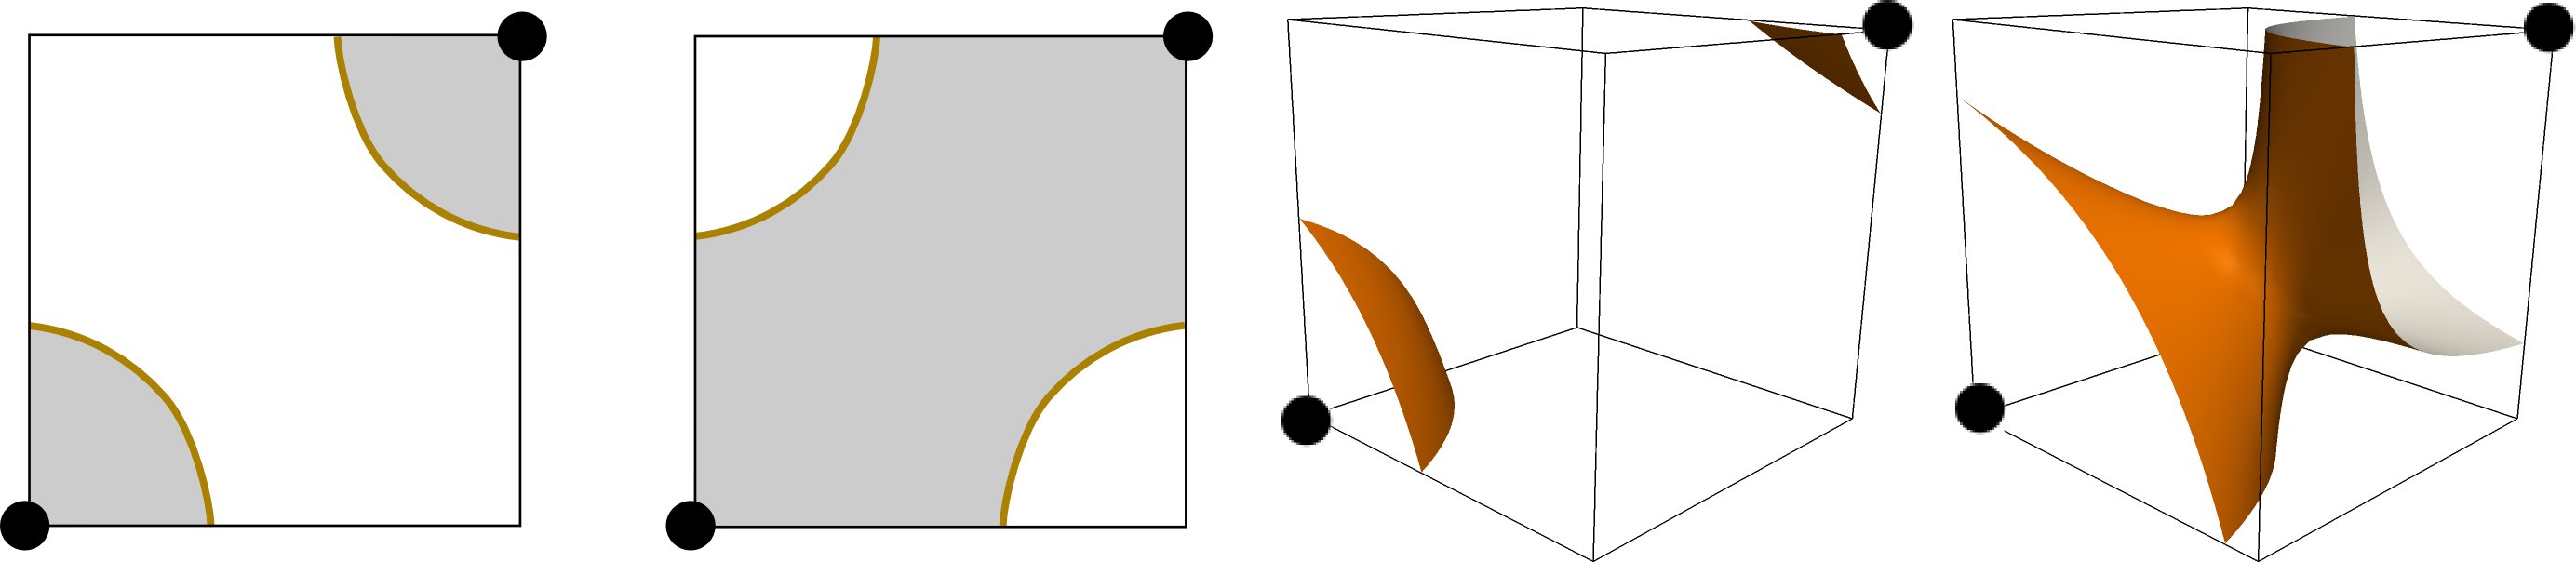
\includegraphics[width=1\linewidth]{chapter4/figures/ambiguity.png}
     \caption{Left: case 4 ambiguity. The interior ambiguity test proposed by Chernyaev is used choose the correct configuration.Right: face ambiguity. The Asymptotic Decider  is used to resolve the ambiguity.}
     \label{ambiguity}
\end{figure}
 
\begin{figure}[t]
     \centering
     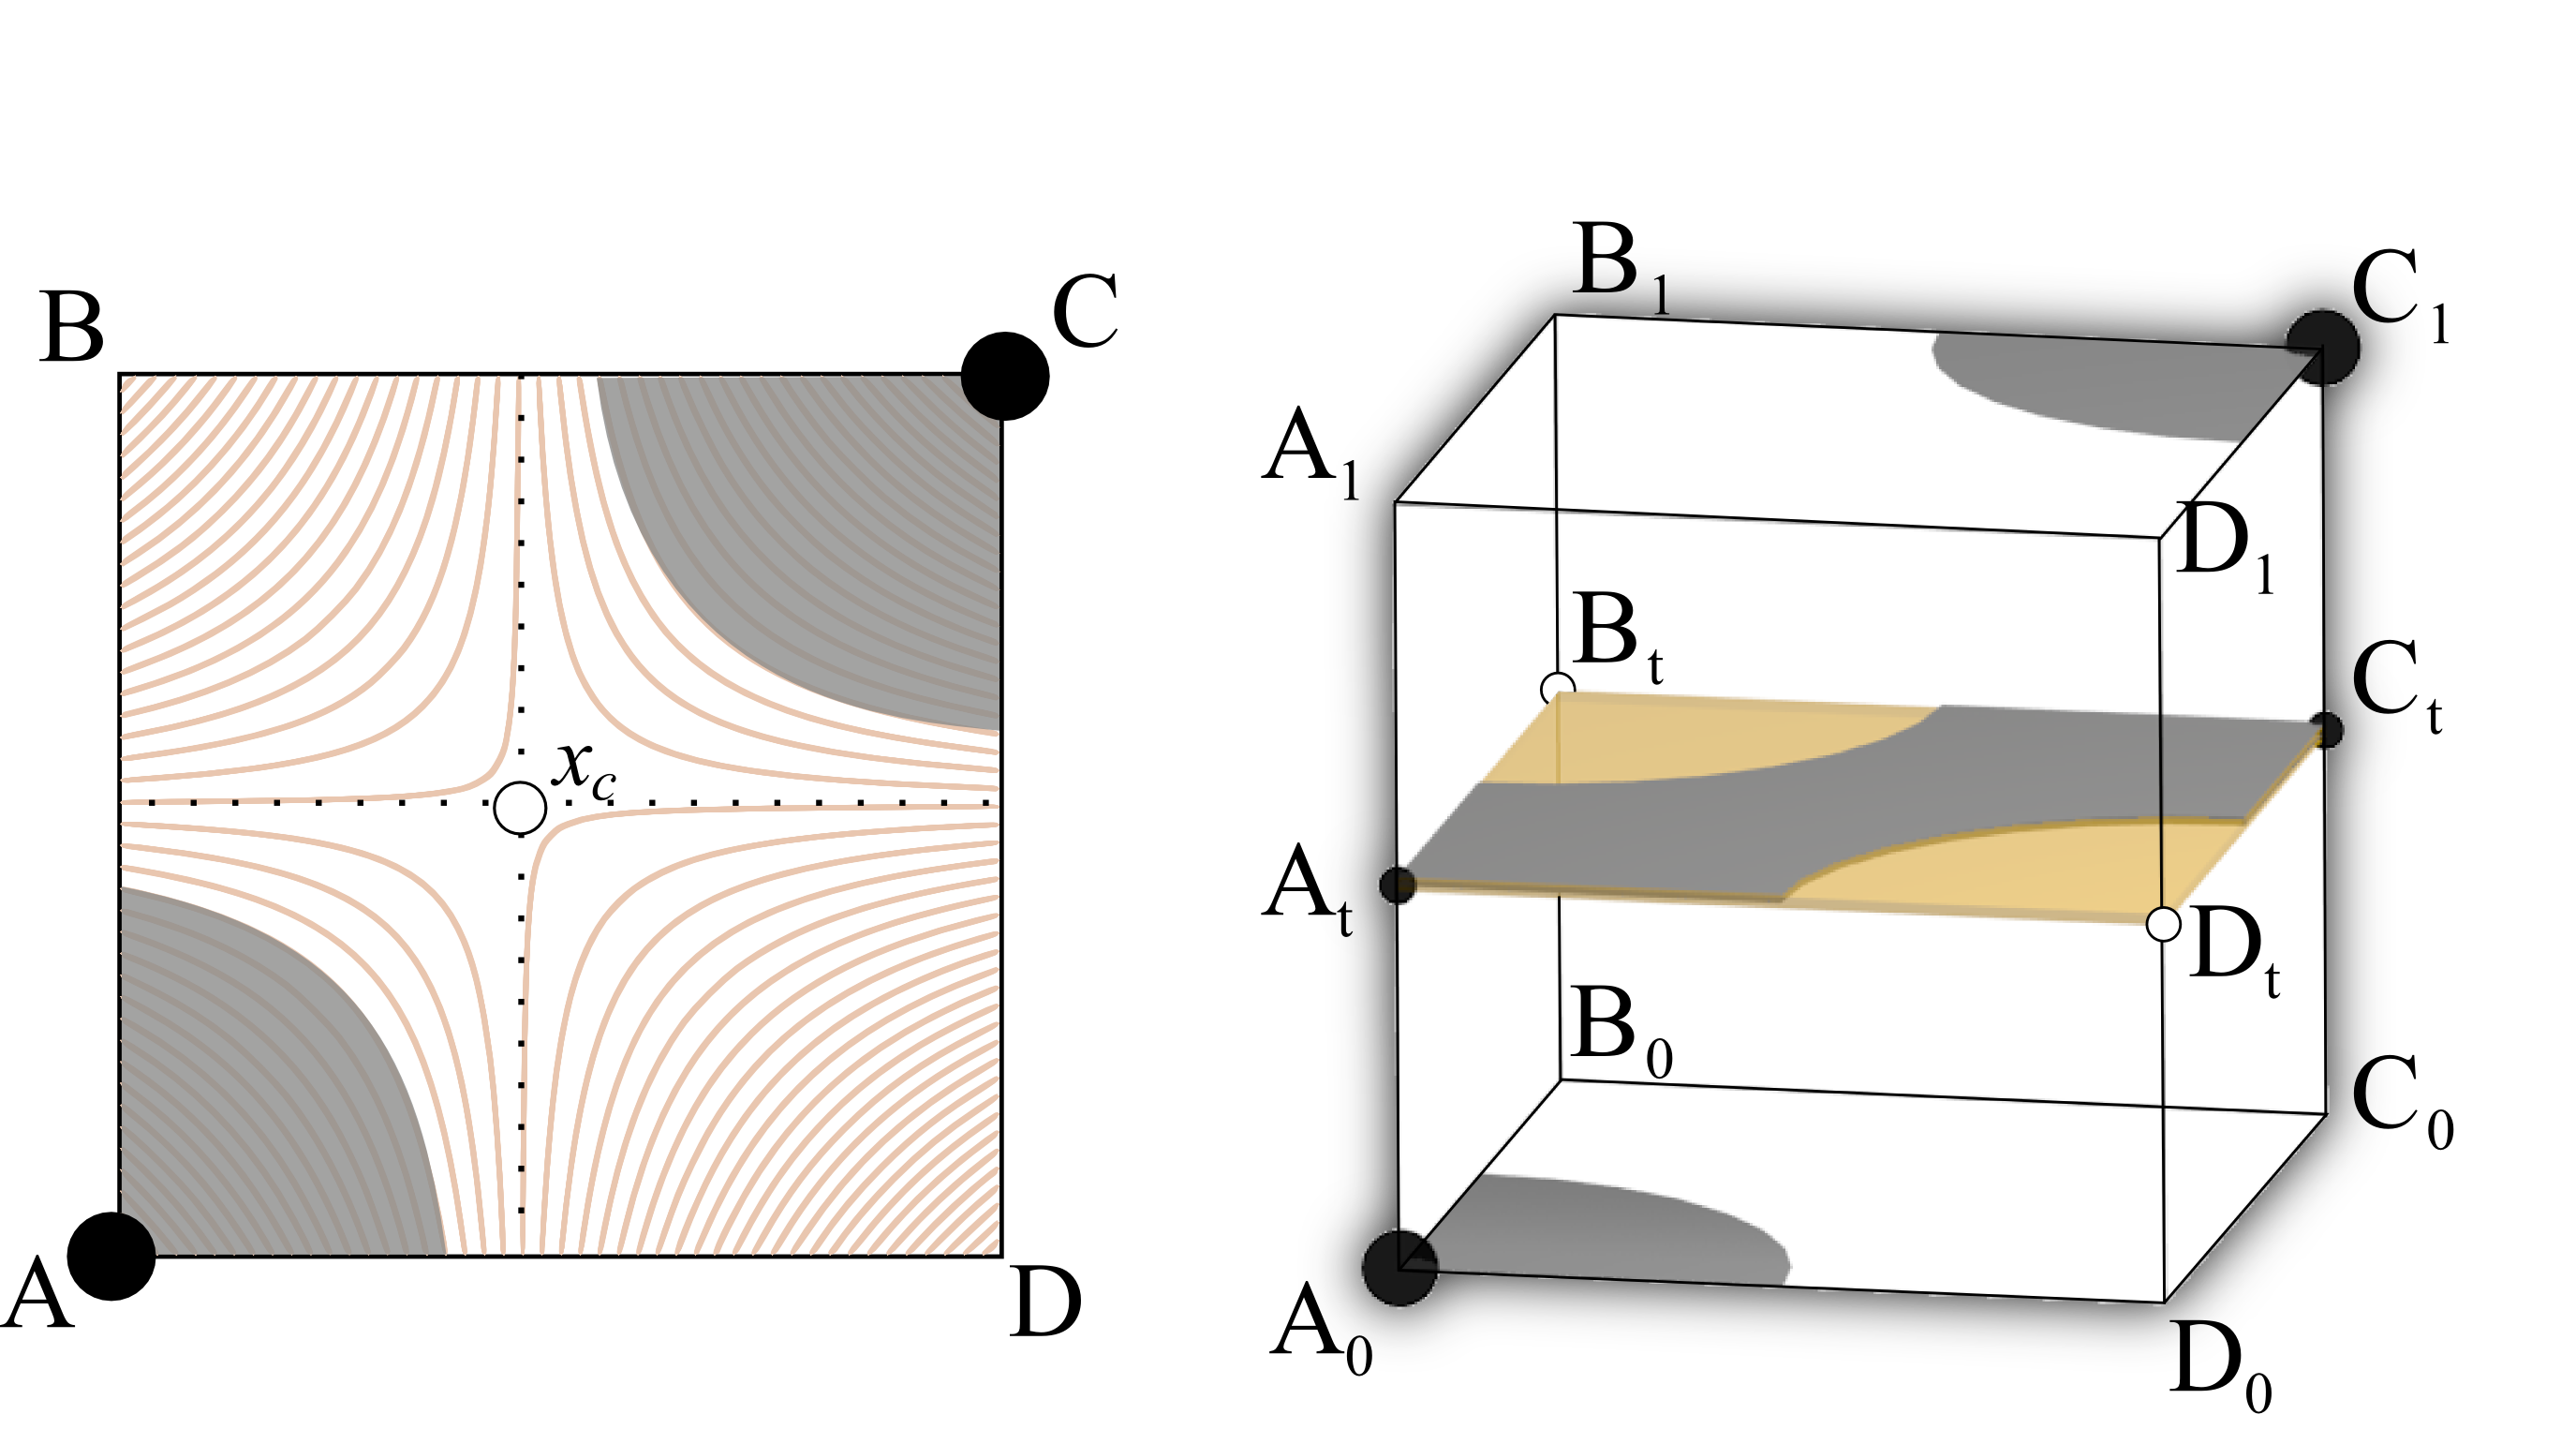
\includegraphics[width=0.65\linewidth]{chapter4/figures/cut-plane-fig.png}
     \caption{Asymptotic Decider (left) and \mc{} interior ambiguity test for MC case 4 (right). The gray areas represent regions with positive scalar values, and the capital letters represent the scalar value at each vertex. In the left image, we observe that $f(x_c) < 0$, where $x_c$ is the saddle point position. Positive areas will be connected if $f(x_c) > 0$. The orange squared plane shown in the right image represents the cutting-plane. The goal of the \mc{} algorithm is to find a cutting-plane such that the gray areas in the top and bottom planes are joined in the interior.}
     \label{interior_ambiguity}
\end{figure}


\subsection{Chernyaev's \mc{}}

The two pillars of Marching Cubes 33's topological correctness are Nielson and Hamann's Asymptotic Decider and Chernyaev's interior ambiguities test; together these solve the face ambiguity and interior ambiguity problems in the Marching Cubes 33 algorithm.
%
A face ambiguity occurs when face vertices have alternating signs. That is, one face diagonal is positive (both vertices are positive) and the other is negative (both vertices are negative). In this case, the signs of the face vertices are insufficient to determine the correct way to triangulate the isosurface. Similarly, an interior ambiguity occurs when the signs of the cube vertices are insufficient to determine the correct surface triangulation, \emph{i.e.}, when multiple triangulations are possible for the same cube configuration (see Figure \ref{ambiguity}).

The idea behind the Asymptotic Decider is to verify the face saddle sign and compare it to the sign on the face vertices. A positive saddle means that the positive face vertices are connected; consequently, the positive face vertices are separated if the face saddle point is negative (see Figure \ref{interior_ambiguity}). To compute the face saddle sign, the saddle point position $x_c$ must be computed~\cite{Chernyaev95marchingcubes}:
\begin{eqnarray}
x_c & = & \left( \frac{A - D}{A+C-B-D}, \frac{A - B}{A+C-B-D} \right), \label{eq:saddle_position}
\end{eqnarray}
where $A$, $B$, $C$ and $D$ are the scalar values at the face vertices (see Figure \ref{interior_ambiguity}).
%
The sign of $x_c$ can easily be checked by replacing Equation \eqref{eq:saddle_position} into the bilinear interpolant:
\begin{eqnarray}
f(x_c) & = & \frac{AC - BD}{A+C-B-D}.\label{eq:saddle_value}
\end{eqnarray}
For an ambiguous face, assuming $A$, $C$ positive and $B$ and $D$ negative, the denominator of the Equation \eqref{eq:saddle_value} is always positive (see Figure \ref{interior_ambiguity}). Then, the face ambiguity is solved by evaluating the sign of the numerator of $f(x_c)$.

Due to the interior ambiguity, the Asymptotic Decider alone cannot solve the topological correctness problem. Chernyaev uses the idea behind the Asymptotic Decider to solve the interior ambiguity problem. The proposed test uses a  sweeping cutting-plane to evaluate the behavior of the trilinear interpolant inside the cube.

Given a cube with an ambiguous configuration, define the scalar values at the base and top planes as $A _{0}$, $B_{0}$, $C_{0}$, $D_{0}$ and $A _{1}$, $B_{1}$, $C_{1}$, $D_{1}$, respectively (see Figure \ref{interior_ambiguity}).  Let $A_{0}$ and $C_{1}$, the vertices to be tested, be positive. Observe that, although $A_{0}$ and $C_{1}$ belong to opposite cube faces, they can be connected through the cube interior. In other words, there may exist a path from $A_0$ to $C_1$ passing through the voxel interior for which all points belonging to that path are positive. To determine whether $A_0$ and $C_1$ are connected, Chernyaev begins by observing that the saddle points at the top and base cube faces are negative, \emph{i.e.}, Equation \eqref{eq:saddle_value} is negative at the bottom and top faces. Since the denominator is positive, it follows that:
 %
\begin{eqnarray}
A_0C_0 - B_0D_0 &<& 0 \label{eq:condition1}\\
A_1C_1 - B_1D_1 &<& 0 \label{eq:condition2}.
\end{eqnarray}

Then, if there is a plane cutting the cube such that its saddle point is positive, it means that there is a positive area crossing the cube,  \emph{i.e.}  the positive vertices are connected inside the cube.  In other words, the Chernyaev interior test searches for a $t$ for which:
\begin{eqnarray}
F(t) = A_tC_t-B_tD_t &>& 0. \label{eq:chernyaev_test}
\end{eqnarray}
This can be achieved by solving a second order equation in $t$. Replacing $X_t = X_0 + (X_1-X_0)t$,  $X \in \{A, B, C, D\}$ and $t \in [0,1]$ in Equation \eqref{eq:chernyaev_test} one obtains a second order equation in $t$:
\begin{eqnarray}
F(t) &=& A_tC_t-B_tD_t\\
       &=& a t^2 + b t + c  \label{eq:disambiguation},
\end{eqnarray}
where $a$, $b$, and $c$ are functions of $A, B, C,$ and $D$ (see \ref{app:counter-example}). Chernyaev concludes that positive vertices $A_0$ and $C_1$ are connected through the cube interior if: 
\begin{enumerate}
\item $a < 0$;
\item $t_{\mathrm{max}} = -b / 2a \in (0,1)$; 
\item $F(t_{\mathrm{max}}) > 0$. 
\end{enumerate}
If one of the above conditions fails, the positive vertices are separated.

\subsection{Lewiner \emph{et al.}'s \mc{}}

Lewiner \emph{et al.}~\cite{Lewiner:2003} proposed a modification of Chernyaev's interior test. In this modification, they use an alternative method for computing the height plane $t$ for most ambiguous cases. For cases  6, 7, 12, and 13, the authors compute the height $t$ based on the barycenter of the end vertices of an edge $e$ (a cube edge intersected by the isosurface) weighted by the values of the scalar field on these vertices (see \cite{Lewiner:2003} for details). In practice, the implementation uses:
\begin{eqnarray}
t_{\mathrm{alt}} &=& \frac{V_{0}}{V_{0} - V_{1}},\label{eq:alternative}
\end{eqnarray}
where $V_{0}$ and $V_{1}$ are the scalar values at the vertices of $e$. Note that this is equivalent to finding the intersection point between the isosurface $S$ and $e$. The authors keep the structure of the test proposed by Chernyaev, but condition (i) is not used, and condition (ii) is always true because $e$ is an edge intersected by the isosurface; consequently, $t_{alt} \in (0,1)$.

Section \ref{erros_cause:chernyaev} explains why the algorithm proposed by Chernyaev and its modified version proposed by Lewiner \emph{et al.} may fail to extract surfaces that are topologically correct. In the following section, we present the tools we use to detect, debug, and reproduce the issues found in the \mc{} algorithm and its implementation. The full Marching Cubes table can be found in the works of Chernyaev \cite{Chernyaev95marchingcubes} and Lewiner \emph{et al.}\cite{Lewiner:2003}.


\section{Experiments setup}
\label{experiments_setup}

We begin by investigating the source of topological problems in the \mc{} implementation~\cite{Etiene:2012:TVI:2197070.2197097}.
%
The topological issues described were obtained by systematically stress-testing the implementation over many topological configurations using the verification framework proposed in Etiene \emph{et al.}~\cite{Etiene:2012:TVI:2197070.2197097}. These authors' algorithm can be summarized as follows.
%
(I) A random scalar field $G$ is built by uniformly sampling scalar values in the range $[-1,1]$ for each $x_j \in G$.
%
(II) The \emph{expected topological invariants} are obtained directly from $S$, {\em i.e.}, without extracting the isosurface of interest. The topological invariants used are the Euler characteristic $\chi(S)$ and the Betti numbers $\beta_k(S)$. 
%
(III) The \mc{} implementation is used to extract a piecewise linear mesh $M$, and its invariants $\chi(M)$ and $\beta_k(M)$ are computed.
%
(IV) Lastly, the pairs of topological invariants $\{\chi(S)$, $\chi(M)\}$ and $\{\beta_k(S), \beta_k(M)\}$ are compared. A mismatch indicates that a problem has occurred. Nevertheless,  as the authors note, a match between invariants does not imply a bug-free code~\cite{Etiene:2012:TVI:2197070.2197097}. The verification process does not prove the absence of bugs but only increases one's confidence in its correctness.
%
In this chapter, we exploit the fact that when the expected and obtained surfaces are not homeomorphic, a counterexample is given in the form of a scalar field $G$ and a mesh $M$. We use this information to find and correct errors in \mc{}.

\subsection{Reproducibility}

\begin{figure}[b]
     \centering
    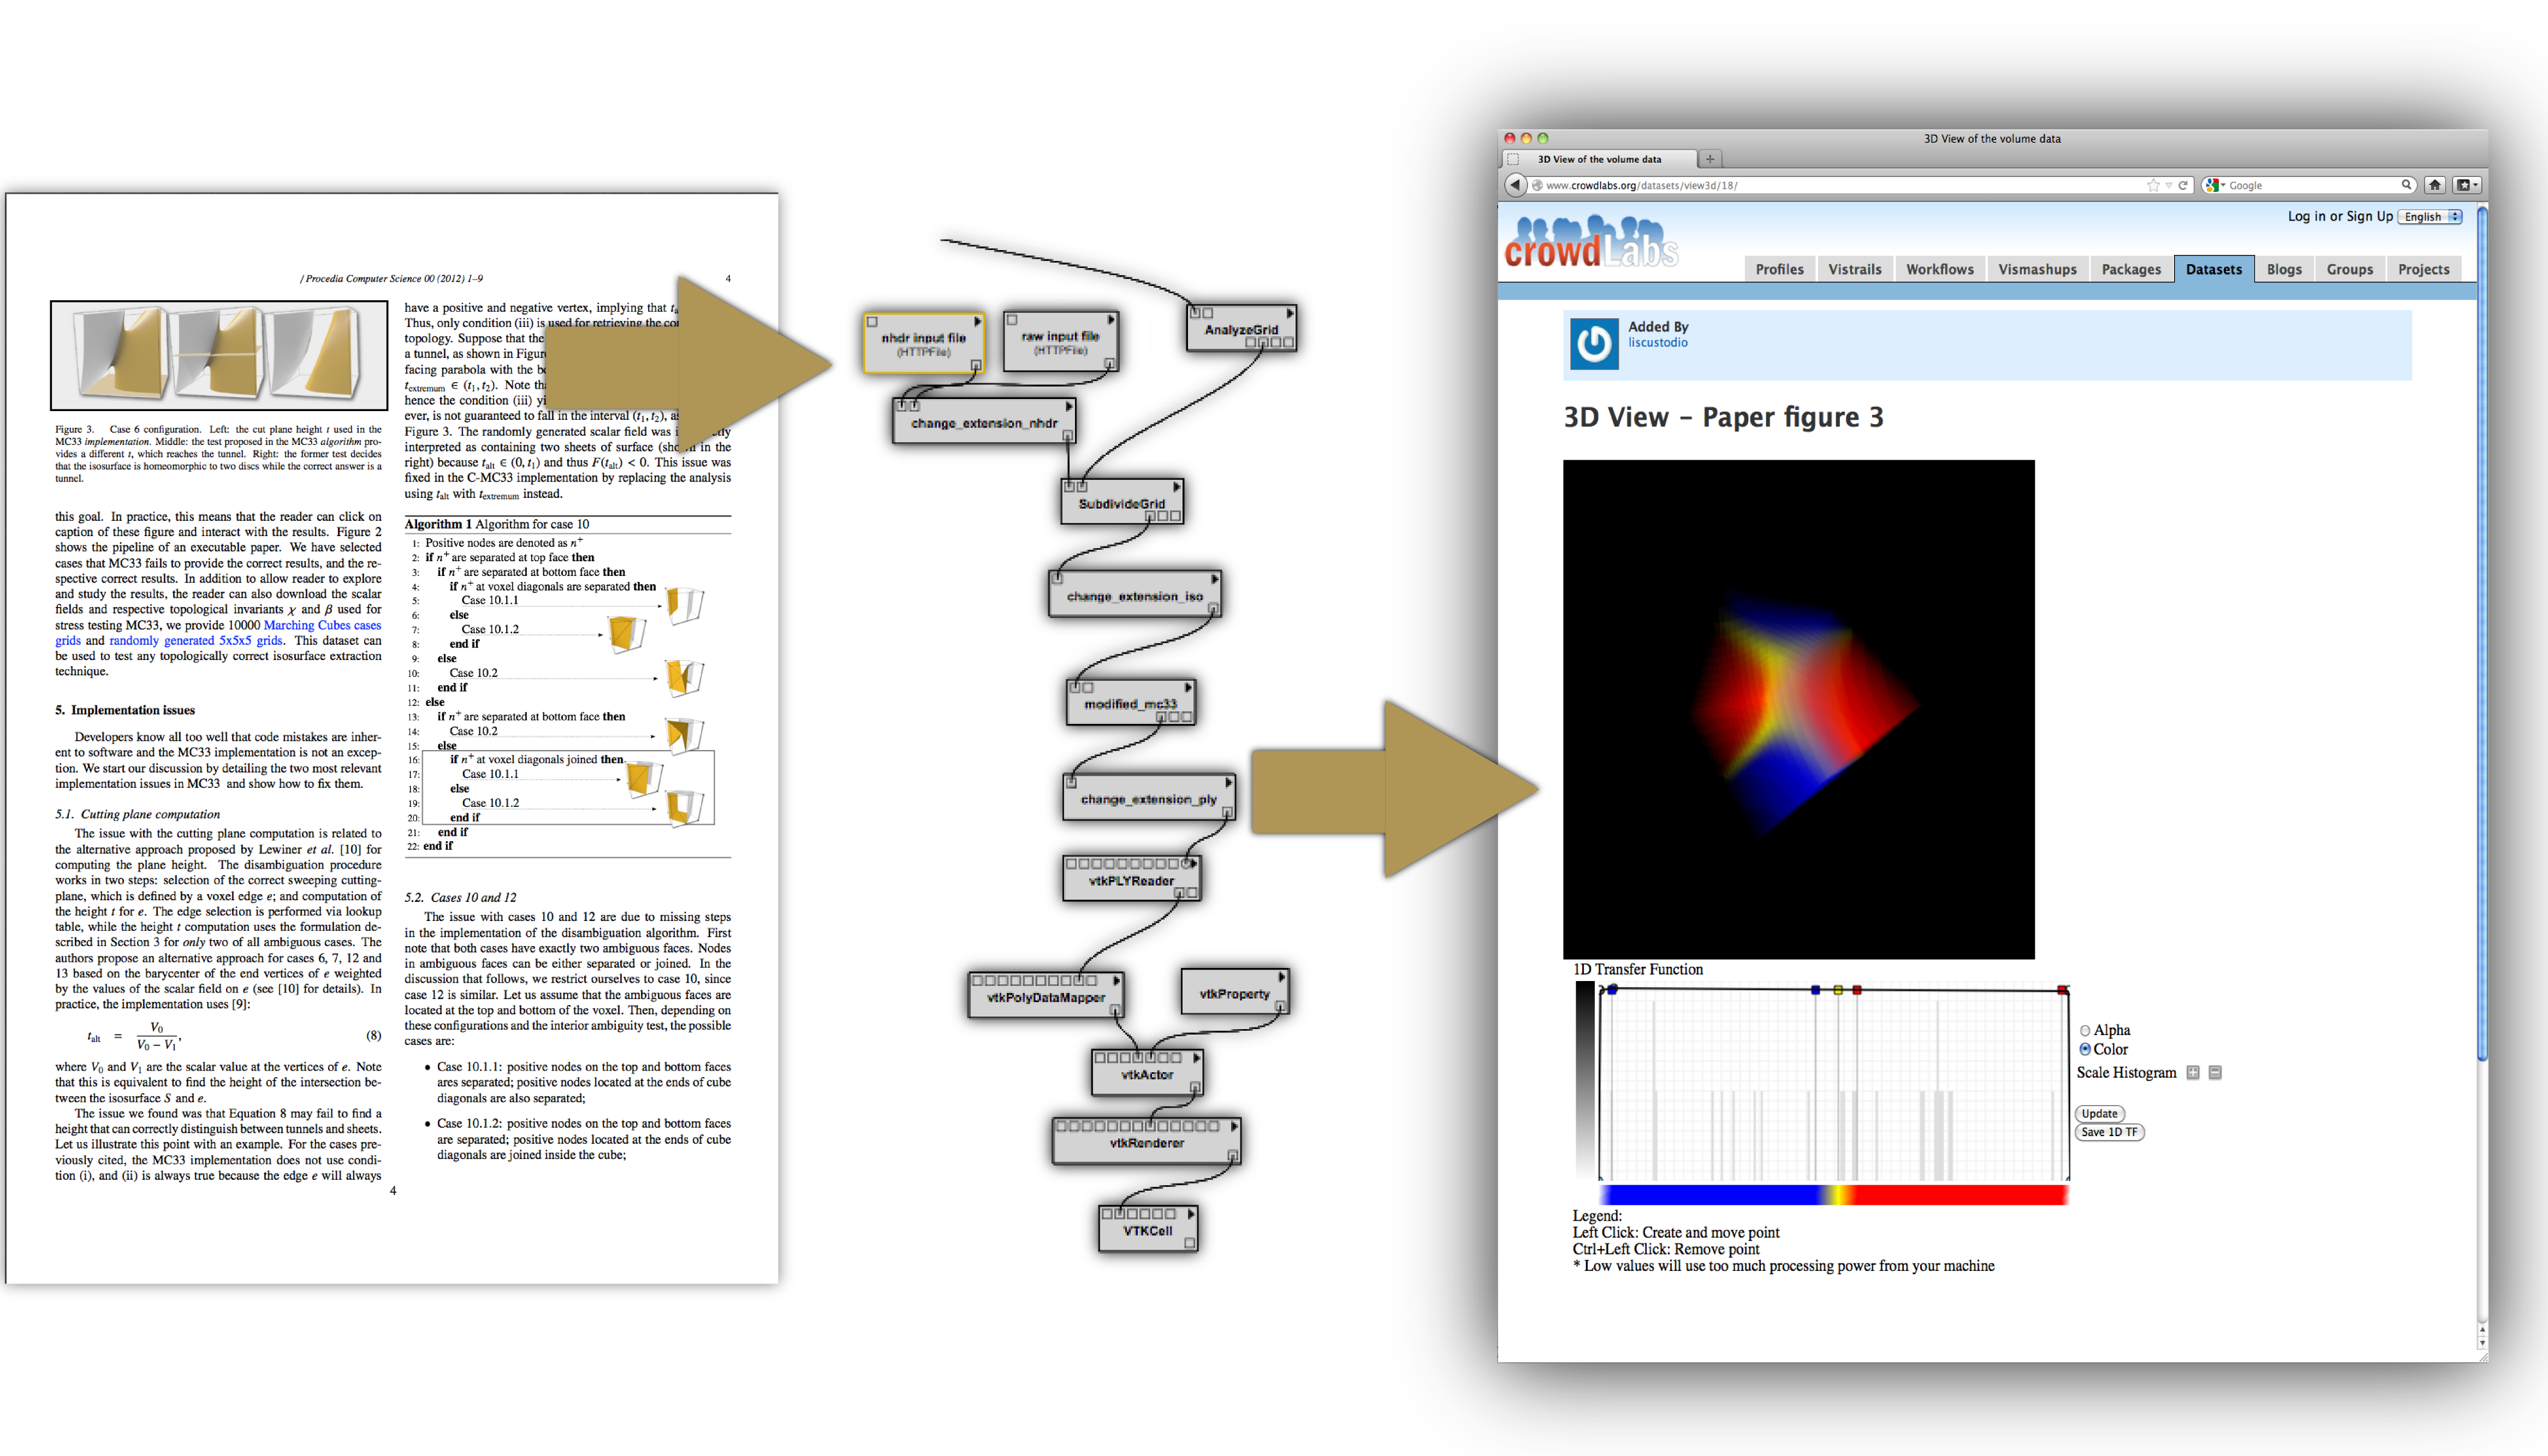
\includegraphics[width=0.7\linewidth]{chapter4/figures/executable.png}
     \caption{ \label{fig:executable}\href{http://liscustodio.github.io/C_MC33/index.html}{The executable paper pipeline. An image is made executable (left), meaning that the reader can launch a request to execute a pipeline in a remote server (middle) and interact with the result in a web browser (right) \cite{lisOnline2013}.}}
\end{figure}

As investigators in a mature field within the scientific visualization community, isosurface extraction researchers have developed ways to help other researchers and practitioners reproduce their results. Published journal articles offer a first approximation of reproducibility. Nevertheless, many details regarding implementation, source code, input data, and other types of information are often omitted. Many, but not all, published techniques make source code and input data freely available, and some are part of widely used visualization packages such as VTK~\cite{vtk}. This practice greatly increases the degree of reproducibility of the work. 
We use CrowdLabs~\cite{Tohline:2010jn} and Vistrails~\cite{Freire:2006va, Silva:2007:PVR:1300781.1302461} as a platform to achieve this goal. To explore some of the results shown in this chapter, the  reader may click on individual figure captions and interact with the results via web browser. Figure \ref{fig:executable} shows the pipeline of an executable paper. 
%
We have selected cases in which \mc{} fails and have provided the respective correct results. In addition,  to allow the reader to explore and study the results presented here, he or she can also download the scalar fields and respective topological invariants $\chi$ and $\beta$ used for stress testing \mc. We also provide 10000 \href{http://liscustodio.github.io/C_MC33/MarchingCubes_cases.zip}{\textcolor{blue}{Marching Cubes cases grids}} and \href{http://liscustodio.github.io/C_MC33/Closed_Surfaces.zip}{\textcolor{blue}{randomly generated 5x5x5 grids}} \cite{lisOnline2013}. This dataset can be used to test any topologically correct isosurface extraction technique.



\section{Issues with the \mc{}}
\label{erros_cause:chernyaev}

In this section, we discuss specific issues regarding both Chernyaev~\cite{Chernyaev95marchingcubes} and Lewiner \emph{et al.}'s~\cite{Lewiner:2003} work. Because Lewiner \emph{et al.} extends Chernyaev's work, the issues presented in the latter are also part of the former. Specifically, we detail three \emph{algorithmic} issues -- two in Chernyaev's \mc{} and one in Lewiner \emph{et al.}  --  and one \emph{implementation} issue. The solutions for the issues raised here will be presented in the next section.

This section is organized as follows. First, we explain an algorithmic problem with the \mc{} core disambiguation procedure. This issue has not been discussed in the literature to date. We then discuss a second algorithmic problem related to the triangulation table and the extraction of non-manifold meshes. Although this problem has been discussed in the literature, we discuss it here for completeness and because we provide an alternative  solution to the problem (see Section \ref{sec:solution}). Next, we show a third algorithmic problem related to the alternative approach proposed by Lewiner \emph{et al.} for computing the height plane $t$. Lastly, we show a non-trivial problem with the open-source implementation of the \mc{}. 

\subsection{Issue I -- Case 13.5}
\label{sec:problem-case-13}

Here, we show a problem with the core disambiguation procedure described in Chernyaev's work. To our knowledge, this problem has not been exposed or addressed in the literature.

Case 13 is certainly the most complex table case; all faces are ambiguous, and six subcases are possible. Four of the subcases can be discriminated by using Asymptotic Decider. The remaining cases 13.5.1 and 13.5.2 require Chernyaev's \mc{} interior ambiguity resolution method.
%
Recall that the \mc{} approach discriminates between tunnels and isolated sheets by finding a cutting-plane for which positive nodes in the cube diagonal are joined by points in the interior of the cubic cell (see Figure \ref{interior_ambiguity}). 
Cases 13.5.1 and 13.5.2 differ precisely because the positive nodes in case 13.5.2 are connected to one another by interior points, which is not true for 13.5.1 (see Figure \ref{fig:case13}).

\begin{figure}[b]
     \centering
     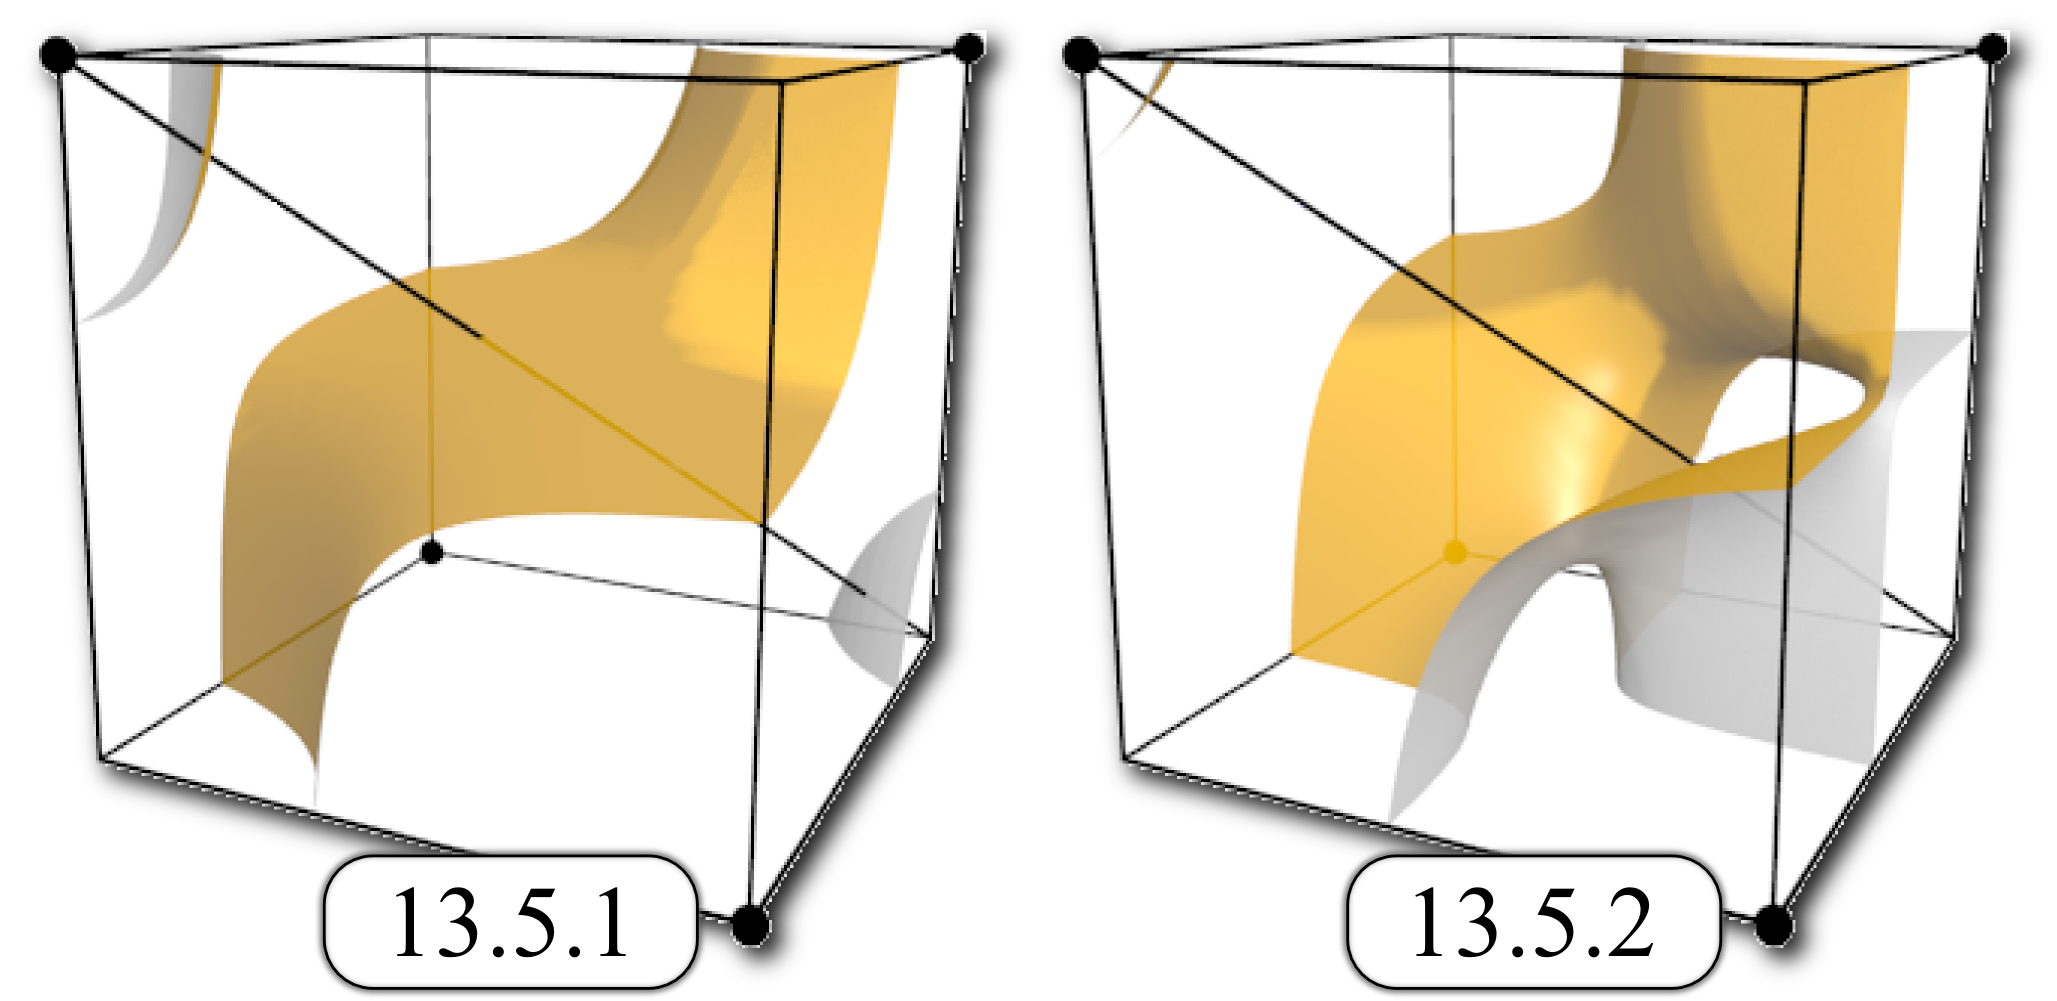
\includegraphics[width=0.6\linewidth]{chapter4/figures/case-13.png}
     \caption{Challenging cases for Chernyave's interior test: voxel diagonal has vertices with opposite signs. Case 13.5.2 needs to be oriented correctly. One of the diagonal vertices is isolated from all other vertices in the cube, while the other is faced by the tunnel. In order to determine which vertex is isolated, we apply the same tool used for disambiguation of case 13.5. For case 13.5.1, the orientation of the isosurface have no influence on the topology. }
     \label{fig:case13}
\end{figure}


\begin{figure}[b]
     \centering
     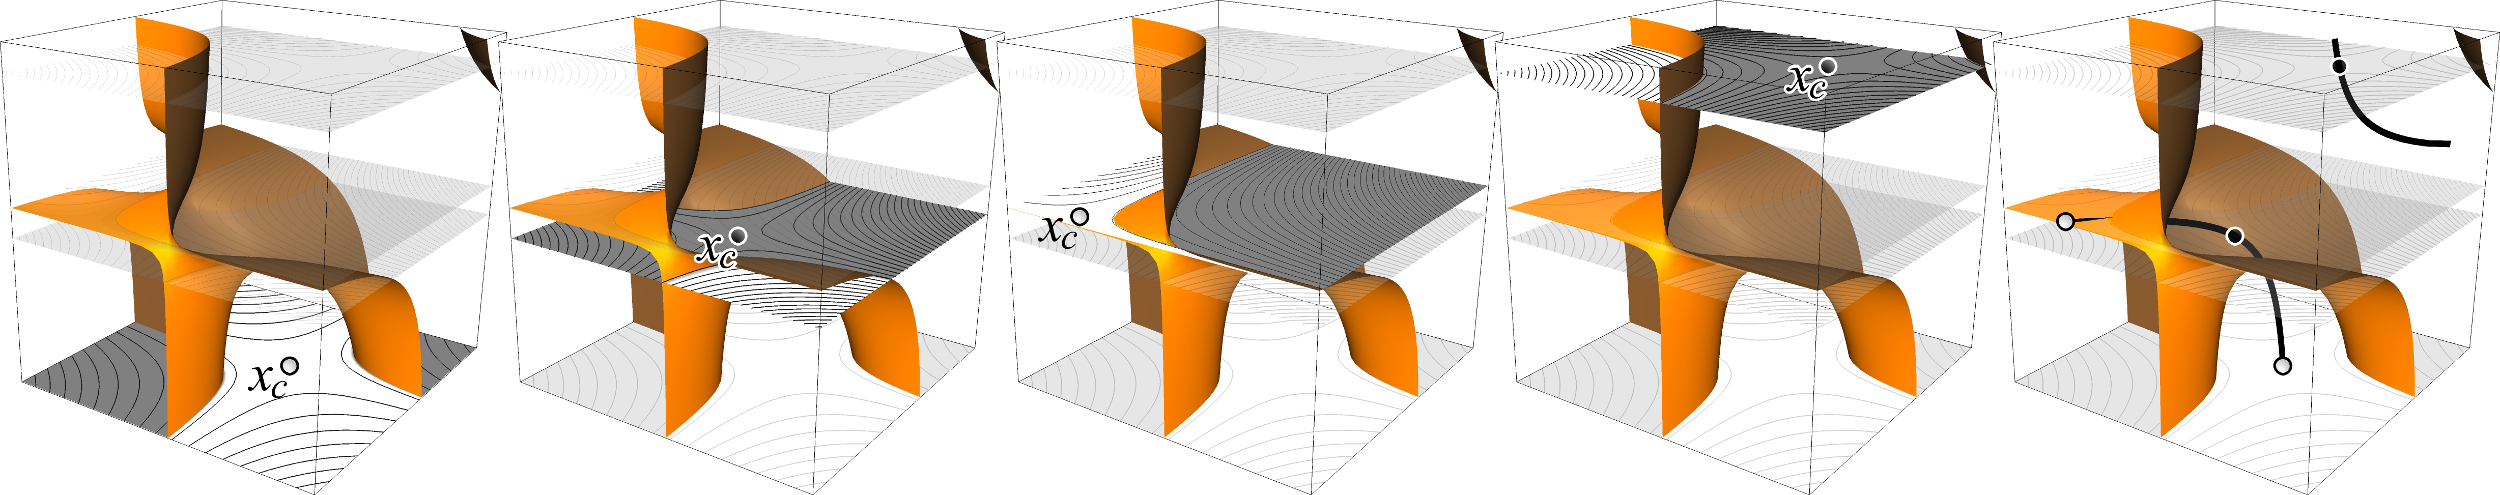
\includegraphics[width=0.99\linewidth]{chapter4/figures/case13/case13.png}
     \caption{Sign changes of the cutting-plane saddle point as a function of the height $t$. The gray area depicts $f(x) > 0$. The black (resp. white) dots are face saddles with $f(x_c) > 0$ (resp. $f(x_c) < 0$). From left to right, the four leftmost images show the sign of the face saddle points changing from negative to positive to negative and to positive again, respectively. The rightmost image shows the  hyperbolic trajectory of the face saddle position $x_c(t)$. The \mc{} algorithm fails to track the saddle point sign because it ignores the influence of the hyperbolic trajectory shown here. }
     \label{fig:case13saddlesigns}
\end{figure}

\begin{figure}[t]
     \centering
     \includegraphics[width=0.7\linewidth]{chapter4/figures//graph.png}
     \caption{Counterexample to Chernyaev's core disambiguation algorithm. The \mc{} algorithm incorrectly interprets case 13.5.2 as 13.5.1. The left image shows the zero-level set for case 13.5.2 and cutting-planes at heights $t_1$, $t_2$, and $t_a$, which correspond to both roots of $F(t)$ and the asymptote of $f(x_c(t))$, respectively. The blue ribbon shows the path of the face saddle $x_c(t)$. The right image shows the changes in $f(x_c(t))$ and $F(t)$. According to the three criteria of the \mc{} algorithm described in Section \ref{sec:preliminaries},  the upward-facing red parabola defines the absence of a tunnel (condition (i)), which is incorrect. The blue curve, on the other hand, shows the correct sign change.}
     \label{fig:case13counter_example}
\end{figure}

Although it seems that the \mc{} methodology described in Section \ref{sec:preliminaries} fits naturally in this scenario, as it turns out this disambiguation procedure \emph{cannot} be applied for 13.5. 
%
Let us illustrate this point with an example. Figure \ref{fig:case13saddlesigns} shows the expected changes in the sign of the saddle point $x_c$ as a function of the height $t$. Mathematically
\begin{eqnarray}
x_c(t) & = & \left( \frac{A_t - D_t}{A_t+C_t-B_t-D_t}, \frac{A_t - B_t}{A_t+C_t-B_t-D_t} \right).
\end{eqnarray}
It follows that the face saddle value (and thus sign) is also defined as a function of $t$:
\begin{eqnarray}
f(x_c(t)) &=& \frac{A_tC_t - B_tD_t}{A_t+C_t-B_t-D_t}\\
       &=& \frac{a t^2 + b t + c}{A_t+C_t-B_t-D_t}.
\end{eqnarray}
As can be seen in Figure \ref{fig:case13saddlesigns}, from left to right, as the plane height $t$ changes, the value of the face saddle $f(x_c(t))$ changes from negative to positive to negative and to positive again. These changes occur at the roots $t_1$ and $t_2$ of $f(x_c(t))$ and the asymptote of $f(x_c(t))$, {\em i.e.}, the root $t_{a}$ of the denominator of $f$ (see left image in Figure \ref{fig:case13counter_example}). Thus, in total, three sign changes will occur. The rightmost image in Figure \ref{fig:case13saddlesigns} shows the path traced by the face saddles $x_c(t)$; as $t$ grows, there is a ``jump'' not only in the sign of $f(x_c(t))$ but also in the position of $x_c(t)$ . The change occurs precisely when the height $t$ passes through the asymptote of $f(x_c(t))$.

Nevertheless, contrary to what is expected, the polynomial $F(t)$ (Equation \eqref{eq:disambiguation}), used by Chernyaev's \mc{} algorithm for tracking the sign of the saddle point, is a second order equation in $t$ and thus can only allow for two sign changes. Therefore, the sign tracked by the \mc{} algorithm will not match the expected one at some point. Because the sign of the saddle points is embedded in all three  conditions for verifying the presence or absence of tunnels, \mc{} will eventually provide a wrong result.

The source of the problem can be tracked to Equations \ref{eq:condition1} and \ref{eq:condition2} and the assumption that the denominator of $f(x_c)$ (Equation \eqref{eq:saddle_value}) is positive. 
These assumptions can easily be verified to be true for case 4, shown in Figure \ref{interior_ambiguity}. However, for case 13, the saddle points at the top and bottom planes have opposite signs, which contradicts Equations \eqref{eq:condition1} and \eqref{eq:condition2}. In addition, the denominator $A+C-B-D$ of $f(x_c)$ changes its sign at the asymptote of $f(x_c)$, contrary to the assumption that it is always positive.
%
The consequence of incorrectly tracking sign changes is that the three rules used for resolving internal ambiguity will fail for some scalar fields. As an example, Figure \ref{fig:case13counter_example} shows a case 13.5.2 that will mistakenly be taken as case 13.5.1 because  $a > 0$ characterizes multiples surface sheets instead of a tunnel (see also \ref{app:counter-example}).
%
The problem is not only related to the misclassification of case 13.5.2 as 13.5.1. We have also devised examples in which case 13.5.1 is mistakenly taken as case 13.5.2 because the three criteria shown in Section \ref{sec:preliminaries} hold. Thus, Chernyaev's interior ambiguity test does not always yield topologically correct isosurfaces.

\subsubsection{Tunnel orientation}

\begin{figure}[b]
     \centering
     \includegraphics[width=0.6\linewidth]{chapter4/figures/tunnel.png}
     \caption{Two possible tunnel orientations for case 13.5.2. The difference between them is the location of the positive vertex.}
\end{figure}
A second minor issue regarding case 13.5.2 is the tunnel orientation of configuration 13.5.2. Once case 13.5.2 is determined, one needs to properly orient the tunnel inside the voxel. The inline figures show the two possibilities. Both vertices at the voxel diagonal are separated from all other voxel vertices at the voxel faces (note that this is not the case for other vertices). Nevertheless, either the positive or the negative vertex of the cube diagonal will connect with vertices with the same sign through the voxel's interior. This will determine which vertex is isolated and which is facing the tunnel. This problem with the tunnel orientation is not dealt with or mentioned in either Chernyaev or Lewiner \emph{et al.}'s work. Nevertheless, it was briefly mentioned in Etiene \emph{et al.} \cite{Etiene:2012:TVI:2197070.2197097}, but no solution to the problem was provided. As the authors observed, the isosurface topology changes if the tunnel orientation is incorrect; thus, it must be oriented correctly. The section \ref{sec:TunnelOrientation} provides a solution for this issue.

\subsection{Issue II -- Non-manifold surfaces}
\label{sec:non-manifold-surfaces}

\begin{figure}[b]
     \centering
     \includegraphics[width=0.9\linewidth]{chapter4/figures/non_manifold.png}
     \caption{\href{http://liscustodio.github.io/C_MC33/figure8.html}{Top: Problem with Chernyaev's triangulation table. The figure shows the  zero level-set of a $5\times5\times5$ randomly generated piecewise-trilinear scalar field $G$ (left) and two meshes extracted using the \mc{} (center) and \cmc{} (right) algorithms. The isolated voxel patches, shown in green and yellow, represent the two voxels at the center of $G$. The face shared by two consecutive tunnels, shown in purple, generates non-manifold edges. After one subdivision at the critical point of this case, the problem no longer occurs, and a valid manifold surface is obtained (right). Bottom: Triangulation for tunnels used by Lewiner \emph{et al.}~\cite{Lewiner:2003}. Each has a face that is coplanar to the voxel faces, which may lead to non-manifold surfaces.} \cite{lisOnline2013}}
  \label{fig:non_manifold}
\end{figure}

The second algorithmic issue is related to the triangulation table used to build triangulated surfaces.
%
The choice of the correct MC configuration is only part of the process of building an algorithm that preserves the topology of the piecewise-trilinear field. The voxel triangulation table is, in fact, the determinant of the final mesh topology.  Chernyaev's original triangulation table contains cases that lead to topologically inconsistent non-manifold meshes in scenarios such as the one shown in Figure \ref{fig:non_manifold}. 
%
This problem occurs because the \mc{} triangulation table allows faces that are coplanar with the grid voxel faces. Hence, when neighbor voxels have ``tunnels'' in their interiors, and share an ambiguous, coplanar face, the end result will be non-manifold edges, as shown in Figure \ref{fig:non_manifold}.
%
Because this is an issue with the triangulation table, any topologically correct algorithm whose table is based on Chernyaev's triangulation table will build non-manifold surfaces whether or not the algorithm can correctly distinguish the voxel cases.

This problem with Chernyaev's work was pointed out by Lopes and Brodlie \cite{lopes:tvcg:2003} (following earlier work by Van Gelder and Wilhelms \cite{Gelder94topologicalconsiderations}) and is one of the motivations of Lopes and Brodlie's work on topologically correct and geometrically accurate isosurface extraction algorithm \cite{lopes:tvcg:2003}. Lopes and Brodlie aimed at improving the geometry quality of the trilinear surface patches and consequently solving the topology problem. They achieve this goal by adding points to the voxel faces as well as to the voxel interior. These extra points are placed on the trilinear patch which increases geometry accuracy. They are classified into three different classes and used for extending the contour of the trilinear patch with the voxel faces. The implementation of this technique becomes intricate and error-prone due to the additional steps required for voxel triangulation. 


\subsection{Issue III -- Cutting-plane computation}

The third algorithmic issue is related to an \mc{} improvement proposed by Lewiner \emph{et al.}~\cite{Lewiner:2003} for computing the plane height.  
The problem is that Equation \eqref{eq:alternative} may fail to find an appropriate height  that can correctly distinguish between tunnels and surface sheets. Let us illustrate this point with an example. For the cases previously cited, two of the conditions in the Chernyaev interior test described in Section \ref{sec:preliminaries} are not used. The \mc{} implementation does not use condition (i), and (ii) is always true because the edge $e$ will always have a positive and a negative vertex, implying that $t_{\mathrm{alt}} \in (0,1)$. Thus, only condition (iii) is used in retrieving the correct voxel topology. Suppose that the scalar field in a given voxel defines a tunnel, as shown in the left image in Figure \ref{interior_test}. In this case, to retrieve the correct topology, $F(t)$ should be a downward-facing parabola with both roots $t_1, t_2 \in (0,1)$, $t_1 < t_2$, and $t_\mathrm{max} \in (t_1,t_2)$. In this case, $F(t) > 0$ only for $t \in (t_1, t_2)$; hence, $F(t_{\mathrm{max}}) > 0$, and a tunnel is retrieved according to condition (iii). The problem with the alternative approach is that, as shown in Figure \ref{interior_test}, the solution to Equation \eqref{eq:alternative} is not guaranteed to fall within  the $(t_1,t_2)$ interval, which implies that the scalar field may be incorrectly interpreted as containing two sheets of surface (shown on the right). In other words, because $t_{\mathrm{alt}} \in (0,t_1)$ and $F(t_{\mathrm{alt}}) < 0$, condition (iii) verifies the absence of a tunnel. 

\begin{figure}[b]
     \centering
    \includegraphics[width=0.95\linewidth]{chapter4/figures/height-plane-problem.png}
     \caption{\href{http://liscustodio.github.io/C_MC33/figure9.html}{\label{interior_test}Case 6 configuration.
     Left: the cut plane height $t = t_{\mathrm{alt}} > 0$ used in the \mc{} \emph{implementation}. Middle: the test proposed in the \mc{} \emph{algorithm} provides a different $t = t_{\mathrm{max}}> 0$, which reaches the tunnel. Right: the former test decides that the isosurface is homeomorphic to two discs whereas the correct answer is a tunnel.} \cite{lisOnline2013}}
\end{figure}

\subsection{Issue IV -- Case 10}
\label{erros_cause:lewiner}

The last issue described in this work is related to the implementation of \mc{}.
Developers know all too well that code mistakes are inherent to software and the \mc{} implementation is not an exception.

Due to a missing step in the implementation of the disambiguation algorithm, \mc{} fails to correctly resolve the ambiguity in cases 10 and 12. Note that both cases have exactly two ambiguous faces and the nodes in ambiguous faces can be either separated or joined. In the discussion that follows, we restrict ourselves to case 10; case 12 is similar. 

Let us assume that the ambiguous faces are located at the top and bottom of the voxel. Then, following the algorithm proposed by Chernyaev \cite{Chernyaev95marchingcubes}, depending on the sign of the face saddles and the interior ambiguity test, one can identify the correct case (see also Algorithm \ref{chernyaev_case10}):
\begin{itemize}
\item Case 10.1.1: the positive nodes on both faces are separated, and the positive nodes at cube diagonals are also separated;
\item Case 10.1.2: the positive nodes on both faces are separated, and the positive nodes at the cube diagonals are not;
\item Case 10.2: the positive nodes are separated on the top and connected on the bottom face.
\end{itemize}

The cases shown above assume that the positives nodes at the top face are separated. But a similar reasoning must be applied to cases in which the positives nodes at the top faces are joined. In the Lewiner \emph{et al.}'s implementation the possibility that the positive nodes at the top faces are joined is missing. 

\section{Solutions}
\label{sec:solution}
 
We present solutions for the four issues raised in the previous section. 
 
\subsection{Issue I -- Case 13.5}

The disambiguation of case 13.5 has been approached in different ways for different frameworks for isosurface extraction.  For example, Nielson \cite{Nielson03onmarching} presents an algorithm that is  concerned with connectivity along edges, faces and the voxel interior. The author presents a detailed description of the behavior of the trilinear interpolant inside the cubic grid and uses these descriptions to solve the ambiguity problem in the interior. Lopes and Brodlie \cite{lopes:tvcg:2003}, on the other hand, use critical points in order to resolve some ambiguities. In this case, the sign of the critical point determines the correct configuration.
%
Unfortunately, the above solutions do not seamlessly integrate with the \mc{} algorithm. The core idea for solving interior ambiguity, namely, that tunnels can be detected by a sweeping plane through the voxel, is absent in both approaches. This motivated us to devise an alternative solution that we feel follows the idea presented in the original algorithm.

We solve this problem by proposing a new interior test that uses the fact that case 13.5.2 requires both \emph{roots} $t_1$ and $t_2$ of $f(x_c(t))$ and the associated saddle points to be inside the voxel. 
%
First, recall that $x_c(t)$ tracks the path of the face saddle inside the voxel as a function of height plane at height $t$, and $f(x_c(t))$ tracks the value (and thus the sign) of that saddle. Both functions are illustrated in the rightmost image in Figure \ref{fig:case13saddlesigns}, in which the black hyperbolic curves represent the path of $x_c(t)$ and the color of the circles represents the sign of the face saddle at a given point (white and black circles are points with negative and positive values, respectively).
%
For case 13.5.2, the path traced by the curve $x_c(t)$ must intersect the isosurface tunnel twice, once at each of the roots $t_1$ and $t_2$ of $f(x_c(t))$. 
%
This implies that both saddle points $x_c(t_1)$ and $x_c(t_2)$ must lie inside the voxel. This is not the case for 13.5.1 because the face saddle can cross the middle sheet at most once. Therefore, it suffices to verify that both roots of $f(x_c(t))$ and its saddle points are inside the voxel. Algorithm \ref{alg:new_case-13} illustrates our solution. Our algorithm is very simple, and does not require the computation of the critical points of the trilinear interpolant, or a detailed description of its behavior inside a voxel. Our algorithm uses the ideas proposed by Chernyaev in order to fix an algorithmic problem in his work.
%
We have implemented and tested this solution on \cmc{} using over 10000 randomly generated instances of case 13.5.

\begin{algorithm}
\begin{codebox}
\Procname{\proc{Case 13.5}($a, b, c$)}
\zi $\rhd$ Let $t_1$ and $t_2$ be the roots of $a t^2 + b t + c$ (Equation \eqref{eq:disambiguation})
\li \If {$t_1, t_2 \in (0,1)$ and $x_c(t_1), x_c(t_2) \in (0,1)^2$} 
\li	\Then \Return Case 13.5.2
\li	 \Else \Return  Case 13.5.1
\End
\end{codebox}
\caption{\label{alg:new_case-13}A simple disambiguation procedure for Case 13.5}
\end{algorithm}

\subsubsection{Issue II -- Tunnel orientation}
\label{sec:TunnelOrientation}

\begin{figure}[b]
     \centering
     \includegraphics[width=0.5\linewidth]{chapter4/figures/case13/solution.png}
     \caption{Solution to the orientation problem. The black dots represent regions with positive scalar values.The cutting-plane location is at $(t_1 + t_2) / 2$. The sign of $f((t_1+t_2)/2)$ determines the tunnel orientation. }
     \label{fig:solution-case13}
\end{figure}

To find the correct tunnel orientation one can use the sign of any point between the roots $t_1$ and $t_2$. This is because any point in this range must have the same sign as the critical points of the trilinear interpolant for case 13.5.2. This can be seen in the black path shown in the rightmost image in Figure \ref{fig:case13saddlesigns} and from the graph in Figure \ref{fig:case13counter_example}. All points between roots $t_1$ and $t_2$ will have the same sign, which is the sign of the ``interior'' of the tunnel. Thus, we compare the sign of $f((t_1+t_2)/2)$ with the sign of both vertices of the voxel diagonal which is inside the tunnel. The tunnel will face the vertex with the same sign as $f((t_1+t_2)/2)$, whereas the other vertex must be isolated from all cube vertices. Figure \ref{fig:solution-case13} illustrates this scenario. Note that Lopes and Brodlie  \cite{lopes:tvcg:2003} used the sign of the critical points of the trilinear interpolant to retrieve the correct tunnel orientation. We provide a different solution that fits nicely with Chernyaev's framework.


\subsection{Issue II -- Non-manifold surfaces}

A possible solution to this problem involves post-pro\-cessing the mesh to remove non-manifold features. Although  many works in the literature proposed methods for fixing meshes (see \cite{springerlink:10.1007/s11390-009-9206-7} for an excellent survey), these are mainly focused on retrieving a valid manifold mesh. Topologically correct algorithms, on the other hand, require that the topology of the trilinear interpolant  be preserved. In addition, mesh repairing techniques may mask implementation issues by fixing them, which complicates the verification process. 

We use an alternative approach that does not require any changes in the \mc{} triangulation table. An interesting fact is that this problem has a low probability of being generated at random and an even lower probability of occurring in real-world datasets. For example, as shown in Figure \ref{fig:non-manifold-real-data} for the Skull dataset this problem appeared six times in total for 50 distinct isosurfaces. In our tests, it occurred only once in 10000 randomly generated $5\times5\times5$ scalar fields. Thus, instead of implementing the approach of Lopes and Brodlie's, we adopt a different solution that takes advantage of the fact that this is a rare event.

Non-manifold surfaces are created when two adjacent voxels that share an ambiguous face have tunnels in the voxel interior. By splitting both voxels at the critical point of that face, the face ambiguity is  eliminated \cite{10.1109/TVCG.2009.10}.
To simplify the algorithm, we split not only the voxels sharing the ambiguous face but all faces in the volume slice that contains that face (see Figure \ref{fig:grid-refinement}). 
%
\begin{figure}[b]
     \centering
	\includegraphics[width=0.5\linewidth]{chapter4/figures/grid.png}
	\caption{\label{fig:grid-refinement}Grid refinement. The slice of voxels containing the offending configuration is splitted into two slices.}
\end{figure}
%
Assuming an input of size $n \times n \times n$, each subdivision will add $n^2$ voxels to the grid.  Assuming that $k$ subdivisions are required, $k n^2$ voxels will be added. In practice $k = O(1)$, and thus $k n^2 = O(1 )O(n^2) = O(n^2)$. This implies that the asymptotic size of the dataset does not change. This subdivision adds the degree of freedom necessary to eliminate the problem, making this implementation of the Marching Cubes 33 topologically correct (see Figure \ref{fig:non_manifold}). 

\begin{figure}[b]
     \centering
     \includegraphics[width=0.9\linewidth]{chapter4/figures/cc_aneurism.png}
     \caption{\href{http://liscustodio.github.io/C_MC33/figure12.html}{Aneurysm dataset. From left to right, the displayed isosurfaces were extracted using VTK, \mc, and \cmc, respectively. We show the main brain artery component in yellow and the extra connected components in purple. From the images shown, it is clear that the purple components should be part of the main branch. Nevertheless, due to the implicit disambiguation in VTK and the issues in \mc, the final isosurface contains multiple components (left and middle figures). The isosurface generated using \cmc{} is shown on the right. } \cite{lisOnline2013}}
     \label{fig:cc_aneurism}
\end{figure}

\subsection{Issue III -- Cutting-plane computation}

Because this is a problem with the alternative method used in Lewiner \emph{et al.}, the issue can be avoided by replacing the use of $t_{\mathrm{alt}}$ with use of the originally proposed $t_{\mathrm{max}}$.

\subsection{Issue IV -- Case 10}

Algorithm \ref{chernyaev_case10} illustrates the required steps for disambiguation on case 10. We fixed the \mc{} implementation by adding the lines 16-20, which in the original implementation were replaced by the result \textit{case 10.1.1}. 

%\begin{algorithm}
%\begin{codebox}
%\Procname{\proc{Case 10}($n^+$)}
%\zi $\rhd$ Let $n^+$ be positive nodes 
%\li \If $n^+$ are separated at top faces 
%\li	\Then \If $n^+$ are separated at bottom face  
%\li		\Then  \If $n^+$  at voxel diagonals are separated 
%\li			\Then 
%\li				\Return Case 13.5.1
%\li			\Else 
%\li				\Return Case 10.1.2
%			\End
%\li		\Else 
%\li			\Return Case 10.2
%		\End
%\li	\Else 
%\li		\If $n^+$ are separated at bottom face 
%\li			\Then 
%\li				\Return case 10.2 
%\li			\Else 
%\li				\If $n^+$ at voxel diagonals are joined 
%\li					\Then 
%\li						\Return Case 10.1.1
%\li					\Else 
%\li						\Return Case 10.1.2
%					\End
%			\End
%	\End
%\end{codebox}
%\caption{\href{http://dl.dropbox.com/u/8414964/C-MC33/webpage/alg2.html}{Algorithm for case 10}}
%\end{algorithm}


\begin{algorithm}
\caption{\href{http://liscustodio.github.io/C_MC33/alg2.html}{Algorithm for case 10} \cite{lisOnline2013}}
\label{chernyaev_case10}
\includegraphics[width=0.7\linewidth]{chapter4/figures/algorithm.pdf}
\end{algorithm}


\section{Experiments with real-world datasets}
\label{sec:real-world}

We now turn our attention to the practical impact of the topological correctness of the trilinear interpolant. 
For real-world datasets, the vast majority of Marching Cubes cases match the non-ambiguous configurations, namely, 1, 2, 5, 8, and 9. This means that the standard Marching Cubes will match the topology generated by both \mc{} and \cmc.
%
Nevertheless, for some voxels, there will be topological differences in the approaches, which may result in quite different meshes. 

For the sake of completeness, in this section we provide a qualitative analysis of these differences. The aneurysm dataset shown in Figure \ref{fig:cc_aneurism} provides an example of the differences. From left to right, Figure \ref{fig:cc_aneurism} shows meshes extracted with VTK Marching Cubes, \mc, and \cmc. The VTK implementation is based on the work of Montani \emph{et al.}~\cite{Montani:1994wp} and does not have topological guarantees aside from consistency. These three implementations can be viewed as three distinct ways of extracting the mesh topology.
%
Although only a handful of voxels differ among the implementations, for the aneurysm dataset the consequence is that the (largest) main brain artery appears quite different in each interpretation. Because the dataset contains several thin features, subvoxel accuracy is required to connect the pieces of the blood vessels. As shown in the inset images in Figure \ref{fig:cc_aneurism}, one voxel is sufficient to separate fairly large vessels.

VTK and \mc{}  generate more extra connected components (shown in purple) than does \cmc. Figure \ref{fig:cc} shows the difference in the number of connected components generated by VTK and \cmc{} (left) and by \mc{} and \cmc{} (right) as a function of the isovalue for the aneurysm dataset. 
%
Clearly, VTK produces substantially more connected components than  \cmc{}  (up to 2400 more components).  The differences between \mc{} and \cmc{} are not as large, although they are sufficient to disconnect important artery segments. In this example, \mc{} generates more  connected components than \cmc{} for most isovalues. 
%
The aneurysm dataset shows that  changes in the topology of some voxels can impact the final surface. 
%
In this particular example, it is reasonable to assume that the blood vessels  form a single connected component and thus that the dataset contains as few connected components as possible. Using this criterion, \cmc{} shows the best performance for most isovalues. 
%
We emphasize that the ``importance'' of the differences in the number of connected components ought to be measured. For instance, although in general \cmc{} produced fewer connected components, for some isovalues the number of components extracted with \cmc{} was greater than the number extracted using \mc{}. As it turns out, this is due to the presence of pieces of small components disconnected from the main artery. However, because small isolated components do not disconnect large portions of the datasets, contrary to what is shown in Figure \ref{fig:cc_aneurism},  \mc{} and \cmc{} could be considered only ``slightly'' different. A thorough study of impact of the different approaches for extracting mesh topology is desirable but is beyond the scope of this work.

The second problem is due to the extraction of non-manifold features. The issue explained in Section \ref{sec:non-manifold-surfaces} also pertains to real-world datasets.  Figure \ref{fig:non-manifold-real-data} shows an example of a medical dataset in which the output of \mc{} implementation is a non-manifold surface. We have observed the same problem for certain isovalues of other commonly used datasets, such as the backpack and bonsai datasets. Nevertheless, in our experiments, this problem occurred  rarely in the datasets tested:  on average, one case of non-manifold edges was found per $10^7$ evaluated voxels.

\begin{figure}[b]
       \includegraphics[width=1\linewidth]{chapter4/figures/aneurism_cc_vtk.pdf}
       \caption{\label{fig:cc} The left plot shows the difference between the number of connected components extracted by VTK implementation of Marching Cubes and the number of connected components extracted by our \cmc{} implementation. The right plot shows the difference in the number of connected components but between the \mc{} and  \cmc{} implementations. Negative values indicate that the \cmc{} implementation generated more connected components.
Clearly, VTK generates more components that \cmc{}. \mc{} generates more components for most of the isovalues. }
\end{figure}

\section{Conclusion}
\label{conclusion}

In this chapter, we discussed in detail three issues with  the Marching Cubes 33 algorithm and one non-trivial issue with its implementation. 
We presented solutions for the issues raised and implement them into \cmc, a topologically correct version of \mc. In addition, we made our results reproducible so that the reader can easily study, explore, and use the results presented here for his or her own purpose. 

\begin{figure}[b]
     \centering
     \includegraphics[width=0.9\linewidth]{chapter4/figures/skull.png}
     \caption{Skull dataset. The image shows a progressive zoom-in into the dataset in order to reveal non-manifold edges. The face containing the non-manifold edges is highlighted  in purple. The rightmost image is an isolated version of the case shown in the dataset, with a slightly different geometry for the sake of clarity. A non-manifold edge appeared six times in total for 50 distinct isosurfaces.}
     \label{fig:non-manifold-real-data}
\end{figure}

\chapter{Verifying Direct Volume Rendering Algorithm}
\label{chap:vr}

\chapter{Flow Visualization}
\label{chap:aiaa}

Flow visualization has been around in some form for as long as people have studied flows.  In some
cases, visualization was done explicitly -- that is, with the expressed purpose of the viewer to highlight
some feature of the flow.  In other cases, it was done tacitly, as when a child looks out the window
of an airplane to see the slip-stream over the wing generated upon take-off.  Visualization has
many roles, spanning from art to science.  In this chapter, we focused on visualization techniques
used for the scientific exploration and explanation of flow phenomena.  In particular, we are interested
in how two communities -- the AIAA community and the Visualization community -- consider
flow visualization.  To accomplish this task, we have used the {\em AIAA Journal} and the
{\em IEEE Transactions on Visualization and Computer Graphics (TVCG)} as ``representative" publication
venues of the two communities, and have explored the papers published therein to try to 
glean how each community approaches visualization of flow, how they might differ from each other, 
and how the two communities might complement each other. 

This chapter is organized as follows.  In Section \ref{sec:flowvis}, we provide a review of the state-of-the-art
in flow visualization, both from the perspective of the Visualization and well as the AIAA communities. 
%
Tools such as Tecplot \cite{amtec1996tecplot} and Paraview \cite{squillacote2007paraview} have implemented many 
standard flow visualization techniques such as LIC (line integral convolution), streamlines, stream ribbons, and more. 
As we will show, our review encompasses much of the current practices in 
flow visualization and also provide pointers to new developments. 
%
In the next two sections, we focus our attention on research advances made within the Visualization 
community that we think will, in time, have impact on flow visualization and on other application domains
that use visualization as a means of both scientific exploration and explanation.  
In Section \ref{sec:perceptionandevaluation}, we show how perception and user studies may impact flow visualization, and
in particular, we focus on
issues related to color maps.  In Section \ref{sec:verif}, we then provide
discussions on the current Visualization community research trends in Visualization Verification 
and Uncertainty Quantification.  We have chosen these topics because they are all related to flow visualization.
%In Section \ref{sec:tools} we review the set of currently
%available tools to fluids researchers, highlighting that some of these tools in fact have some of the
%advanced features of the Visualization Community, even if the general user-base is not aware.
In Section \ref{sec:opportunities}, we speculate on some of the opportunities for collaboration and
more effective communication between the two communities, and we conclude in Section
\ref{sec:conclusions}.

%%%%%%%%%%%%%%%%%%%%%%%%%%%%%%%%%%%%%%%%%%%%%%%%%%%%%%%%%
\section{Review of Flow Visualization Techniques}
\label{sec:flowvis}

%* Intro
%* Review of flow vis 
%	- Vis community
%	- AIAA community
%* How mature is the flow vis field? Evaluation, Uncertainty, and Verification of flow vis techniques.
%      - Here we show a plot of the new wave of evaluation papers/user studies inside the Vis community
%* Opportunities:
%	- Does the Vis community knows the problems and challenges faces by AIAA community?
%	- Does the AIAA community knows the advances made by the Vis community?

Vector field visualization is an important and vibrant subfield of both the Visualization and AIAA communities.
%
The techniques developed for vector field visualization extend beyond these communities to fields such as medical imaging, meteorology, the automotive industry, and others.
%
In the past two decades, visualization experts and practitioners have seen the development and improvement of many vector field visualization techniques.
%
The contributions are numerous: the ability of handling different grid types (structured, unstructured, curvilinear, etc), high dimension data (2D, 2.5D, and 3D), time-dependent flow, seeding and placement of geometric primitives, improved performance, perception, rendering, among others.
%
In this section, we review some of the developments inside the Visualization community and compare with current practices inside the AIAA community.

\subsection{Preliminaries}

Although the concept of flow visualization is well defined in both communities, we start by clarifying what is meant by flow visualization in this section.
%
The difference between \emph{computational flow visualization} and \emph{flow visualization} is that the latter focus on visualization of flow behavior using experimental data (\emph{e.g.}, flow in a wind tunnel), whereas the former visualizes flow from simulated or computed data. 
%
Some computational visualization techniques are inspired by techniques used in flow visualization, such as dye advection. 
%
Since the subject of this section only addresses computational flow visualization, we will refer to that topic simply as flow visualization.

For thoroughness, we also define some commonly used mathematical/physical terms used within the flow visualization literature.
A \emph{streamline} is the path traced by a massless particle in a steady flow. Streamlines are sometimes referred to as ``instantaneous particle trace''.
%
A \emph{streakline} is the path traced by massless particles seeded at the same position but at different times in a unsteady flow. 
%
\emph{Stream surfaces} and \emph{streak surfaces} are the 2-manifold analog of streamlines and streakline, where the seeding primitive is a curve instead of a point.

\subsection{Classes of Techniques}

\begin{table}
\caption{\label{table:progress}Advances in flow visualization. This table is \emph{not} meant to be comprehensive.}{}\centering
\begin{tabular}{c c r p{7.25cm}}
\toprule
Class &  Subclass & Technique & Reference\\
\hline
\multirow{5}{*}{\bf Direct} 	&\multirow{4}{*}{\em Arrows}		& \cc Standard  & \cc Klasshen and Harrington \cite{Klassen:1991:SHT:949607.949631} \\
					&							& \cc Hybrid  	& \cc Color-coding and arrows \cite{Kirby:1999:VMD:319351.319429}\\
					&							& \cc 3D  			& \cc Arrows in 3D space, 2-manifolds embedded in 3D \cite{Peng:2012:MVF:2086335.2086624}\\
					&							& \cc Enhancements& \cc Large data \cite{Peng:2012:MVF:2086335.2086624}, resampling \cite{Laramee2003905}\\
					&\multirow{1}{*}{\em Color coding}	&  Standard	&  Color maps, volume rendering \cite{Engel:2004:RVG:1103900.1103929}\\
\hline
\multirow{8}{*}{\bf Geometry}	&\multirow{5}{*}{\em Curve}	& \cc Streamline  	& \cc Turk and Banks \cite{Turk:1996:ISP:237170.237285}\\
						&						& \cc Seeding		& \cc User-assisted \cite{Jobard97creatingevenly-spaced}, automatic \cite{MebarkiAD05,li2008illustrative}, and hierarchical \cite{jobard2001multiresolution}\\
						&						& \cc 3D			& \cc 2-manifolds embedded in 3D \cite{spencer2009evenly}\\
						&						& \cc Rendering	& \cc Illuminated \cite{Mattausch:2003:SIE:984952.984987}, streamtubes and streamribbon \cite{Ueng:1996:ESS:614262.614333}\\
						&						& \cc Unsteady		& \cc Wiebel and Scheuermann \cite{wiebel2005eyelet}\\
						&\multirow{3}{*}{\em Surface}	& Stream surface  	& Hultquist \cite{Hultquist:1992:CSS:949685.949718}\\
						&						& Enhancements	& Seeding and placement \cite{Peikert:2009:TRS:1980462.1980472}, accuracy \cite{Garth:2008:GAI:1477066.1477441}\\
						&						& Unsteady		& Schafhitzel \emph{et al.} \cite{Schafhitzel:2007:PSS:1268517.1268564}\\
\hline
\multirow{8}{*}{\bf Texture}&\multirow{5}{*}{\em LIC}		&\cc Standard		&\cc Cabral and Leedom \cite{Cabral:1993uu} \\
					& 							&\cc Performance	&\cc Improved algorithm, parallelism, real-time, GPU \cite{Li:2006:GIA:2384796.2384800}\\
					& 							&\cc 3D			&\cc 3D and 2-manifolds embedded in 3D \cite{10.1109/TVCG.2010.121}\\
					& 							&\cc Rendering		&\cc Flow orientation cues, local velocity magnitude\\
					& 							&\cc Unsteady 		&\cc Li \emph{et al.} \cite{Li:2006:GIA:2384796.2384800}\\
					&\multirow{3}{*}{\em Spot Noise}	& Standard			& van Wijk \cite{vanWijk:1991vd} \\
					& 							& Enhanced 		& It deals with highly curved/high velocity vector fields. \cite{deLeeuw:1995tp} \\
					& 							& Performance		& Parallel implementation. \cite{Leeuw:1997vr} \\
\hline
\multirow{6}{*}{\bf Feature}	&\multirow{4}{*}{\em VFT$^{*}$}	&\cc Standard		&\cc First-/High-order critical point tracking \cite{Helman:1989:RDV:72885.72887,de1999visualization,Scheuermann:1998:VNV:614270.614397} \\
						& 							&\cc Compression 	&\cc Theisel \emph{et al.} \cite{CGF:CGF680}\\
						&							&\cc Simplification	&\cc Weinkauf \emph{et al.} \cite{weinkauf05a}\\
						& 							&\cc Streakline 		&\cc Weinkauf and Theisel \emph{et al.} \cite{Weinkauf:2010:SLT:1907651.1908009}\\
						&\multirow{1}{*}{\em STD$^{**}$}	& Pathline			&Theisel \emph{et al.} \cite{Theisel:2005:TMT:1070610.1070741} \\
						&\multirow{1}{*}{\em LM$^{***}$}	&\cc FLTE			&\cc Haller \cite{Haller:2001:DMS:370169.370176},  Garth \emph{et al.} \cite{Garth:2007:ECV:1313046.1313106}\\
\hline
\multicolumn{4}{l}{$^{*}$ Vector Field Topology $^{**}$ Space-Time Domain $^{***}$ Lagrangian Method}\\
\bottomrule
\end{tabular}
\end{table}

Flow visualization techniques can be classified as direct, geometric, texture-, and feature-based (see Figure \ref{fig:classes}). 
%
Table \ref{table:progress} provides an overview of the classification and a subset of the available techniques within each class.  
%
The table provides a hierarchy of the flow visualization tools available.
%
The \emph{Subclass} column provides the main component of a given visualization techniques that can be found within the \emph{Technique} column.
%
One can find reference to extra material within the \emph{Reference} column. 
%
For more details about the articles shown in Table \ref{table:progress} and others, we refer the interested reader to the excellent surveys by Hauser \emph{et al.} \cite{Hauser:2003tm} and Peng and Laramee \cite{peng2009higher} for an overview of the flow visualization field, Edmunds \emph{et al.} \cite{Edmunds2012974} and McLoughlin \emph{et al.} \cite{CGF:CGF1650} for geometric flow visualization, Laramee \emph{et al.} \cite{laramee2004state, laramee2008applications} for texture-based flow visualization, and Pobitzer \emph{et al.} \cite{CGF:CGF1901} for feature-based flow visualization. 
%
Next, we briefly go over each of the classes.


\begin{figure}[b]
\centering
\includegraphics[width=1\linewidth]{chapter6/figures/classes.png}
\caption{Examples of flow visualization using direct, geometry, texture-, and feature-based techniques, respectively.}
\label{fig:classes}
\end{figure}


%%%% Direct visualization
\subsubsection{Direct visualization} 
%
Direct visualization techniques provide an intuitive and straightforward way of visualizing vector fields. 
%
In this approach, primitives of interest -- such as arrows, glyphs, or lines -- are placed at (often regularly-spaced) seed points. 
%
The primitives are then oriented according to the vector field. 
%
Optionally, the vector magnitude can be mapped to the primitives via scaling. 
%
%Although the research into direct visualization has slowed down in recent years, the work by Peng \emph{et al.}\cite{Peng:2012:MVF:2086335.2086624} is a recent development combining vector field clustering for unstructured grid and glyph placement on boundary surfaces. 
%
Other flow properties, such as pressure and vorticity, can also be mapped using color maps.
%
In the 3D case, volume rendering \cite{Engel:2004:RVG:1103900.1103929} is the natural choice for mapping flow properties into color and transparency.
%
Although direct visualization provides an easy first approximation of the vector field, the visual complexity and occlusion may impair the interpretation of the results, especially in 3D datasets.

%%%% Geometric visualization
\subsubsection{Geometric visualization} 
%
In geometric visualization, curves and surfaces are used for summarizing flow behavior at particular seed points.
%
Geometry-based approaches requires a more intensive processing of the data before the visualization than direct approaches. 
%
The main idea behind integration-based geometric flow visualization is to trace particles or curves through the vector field. 
%
By tracing particles (or respectively curves) one builds a 1-manifold (or respectively a 2-manifold) that can later be visualized.
%
Geometric visualization techniques have a two steps: first, geometry computation; and secondly, rendering. 
%
Often, the rendering step is straightforward -- \emph{e.g.}, rendering a polyline -- in which case the algorithm collapses into one step.
%
Streamlines are one of the most well-known representative visualization tools within this class. 
%
Although flow visualization using both curves and surface dates back over two decades, in recent years, there has been constant research on the topic \cite{Edmunds2012974}. 
%
%Some of the challenges that have been tackled are the problems of occlusion, seeding and placement of primitives, and rendering.
%
% Curves
For curves, the main contributions of the past decade are related to rendering, seeding and placement of curves.
%
% Surface
Edmunds \emph{et al.} \cite{Edmunds2012974} classify the surface-based flow visualization into surface construction and rendering. 
%
Methods for surface construction are based on integral surface, implicit, and topological construction. 
%
This is an area of intense research in the past few years.
%
The authors present a variety of algorithm for both steady and time-dependent surfaces. 
%
Surface rendering methods involve the use of several techniques for improving the quality of the visualization of the flow over a surface of interest. 
%
Surface-based techniques can take advantages of direct or texture-based methods by including static/animated arrows over stream surfaces, shading for the evaluation of the shape of surfaces, placing streamlines over 3D surfaces, employing line-integral convolution (LIC) techniques, and/or nonphotorealistic rendering techniques.

%%%%% Feature-based visualization
\subsubsection{Feature-based visualization} 
%
In feature-based flow visualization, the input vector field is segmented according to features of interest. 
%
As an example, consider a segmentation using classical vector field topology in 2D \cite{Helman:1989:RDV:72885.72887} (see also the right image in Figure \ref{fig:classes}). 
%
Let us assume that the features of interest are first order critical points, namely, focus source, focus sink, node source, node sink, and saddles. 
%
A segmentation is performed by building a topological skeleton through the computation of the vector field's separatrices.
%
The final result provides a cleaner representation of the flow behavior in terms of the aforementioned features.
%
The intensive processing of extracting features before visualization brings many advantages to the practitioner.
%
First, feature-based techniques are valuable for visualization purposes: 
%
feature extraction provides an excellent level of abstraction of the data by removing undesired features and focusing the viewer on the important regions of the dataset.
%
In addition, it can be used for vector field compressing, topological simplification, and even for building custom vector fields \cite{theisel2008}. 
%
Topology-based approaches for feature-based visualization is not the only methodology available.
%
In Lagrangian methods, the trajectories of particles are used to describe and segment the fluid flow.
%
In particular, FLTE \cite{Haller:2001:DMS:370169.370176} methods have gained prominence as a research area within the last decade.
%
One advantage of Lagrangian methods over traditional vector field topology is that they can naturally deal with unsteady flow \cite{CGF:CGF1901}. 
%
Space-time domain techniques are another example of feature-based visualization.
%
In this approach, in order to deal with the problems involved in unsteady flows, the problem of 2D and 3D flow visualization is moved to higher dimensions.
%
As an example, time-dependent domains are merged into a single dataset where traditional techniques used for steady vector fields can be employed.
%
A comprehensive survey on the topic can be found in the state-of-the-art report by Pobitzer \emph{et al.} \cite{CGF:CGF1901}.


%%%%% Texture-based visualization
\subsubsection{Texture-based visualization} 
%
In texture-based flow visualization, the user replaces geometrical information with 2D texture mapped over surfaces. 
%
Line integral convolution (LIC) is a well-known (within the visualization community, at least) representative of the class. 
%
Texture-based techniques generate what is considered a dense visualization, \emph{i.e.}, it covers the entire domain of interest,
%
%\footnote{This is not ideal for all kinds of tasks, as suggested in previous user study where participants performed worse when using LIC \cite{cite study where LIC performs worse than other 2D flow vis}}
%
and it does not have to deal with the problem of finding appropriate seeding spots for streamlines. 
%
Texture-based techniques can be applied along with geometric or feature-based visualization; for instance, it can be used to render flow on 2-manifolds embedded in 3D spaces, or providing an overview of the flow behavior along with topological skeletons.
%
The main issue with texture-based visualizations is the high computational cost associated with it. 
%
Nevertheless, the advances in both computer hardware and algorithms have granted to users the ability to handle large data sets and unstructured grid at interactive rates \cite{Edmunds2012974, laramee2008applications}.

\subsection{Means to an End}
%% Stats:
%Grid Type Used: Cartesian, Unstructured, Curvilinear, B-Spline Volumetric Mesh, Quad-tree
%Domain: 2D, 3D, and 2-manifold embedded in 3D space
%Papers containing at least one flow visualization technique: 78
%2D Contour and 2D color maps were left out because they appear in too many papers
%3D streamlines/streamtrace/pathline: 15	
%2D streamlines/streamtrace/pathline: 33
%3D Contour: 27
%2D Glyphs/Arrows: 24
%3D Glyphs: 2
In his position paper ``On the death of visualization'' \cite{citeulike:4186603}, Lorensen argues for the need to bring visualization researchers closer to experts and practitioners. 
%
We have run a simple experiment in order to attempt to ascertain ``the distance" between the Visualization and AIAA communities.
%
We evaluated 78 articles published within the {\em AIAA Journal} over the period of Jan/2010-Oct/2012 containing at least one flow visualization image. 
%
Then, we simply counted the number of papers that contained at least one occurrences of the techniques shown in Table \ref{table:progress}. 
%
We did not include the 2D color mapping and 2D isocontour visualizations as they appear quite often. 
%
Since multiple visualization techniques can be used in a single article, the percentages shown below are just the fraction of publications containing at least one particular type of visualization.
%
Particle tracing using integration-based geometric visualization techniques for 2D vector fields is the most commonly used technique ($42\%$), followed by 3D isocontouring ($35\%$), 2D and 3D arrows and glyphs ($33\%$), and 3D particle tracing ($19\%$). 
% 
Excluding isocontouring (which is mainly used for depicting scalar, instead of vector, data), $61\%$ of the articles used at least one geometric approach to flow visualization, whereas $33\%$ used a direct approach. 
%
Finally, $73\%$ of the papers contained at least one visualization for 2D domains, whereas this number is $56\%$ for 3D domains. 
%
The latter number drops to $22\%$ if one considers only techniques for visualization of vector field data (\emph{i.e.}, excluding 3D isocontouring).

Although the data are limited to a short window of time, they raised a few interesting points. 
%
With the exception of a handful of papers, most of the flow visualization appears to be using the standard form of the traditional visualization technique.
%
As an example, consider some the papers that use streamlines for visualizing 3D flow. 
%
It may be the case that a subset of these paper can benefit from using stream ribbons \cite{Ueng:1996:ESS:614262.614333}, which simultaneously encode the streamlines path and local flow vorticity,
%
or from stream tubes \cite{Ueng:1996:ESS:614262.614333}, which simultaneously encode the streamlines path and local cross flow divergence. 
%
Both stream ribbons and stream tubes are well-known, and commonly used visualization packages such as Paraview or Tecplot have them available within their tool options.
%
%
%
%
Secondly, the preference for the two visualization techniques (direct and curve-based geometric visualization) shown in past three years is perhaps due to their simplicity and availability. 
%
The underrepresented methods in the same period of time are texture-, feature-, and surface-based flow visualization.
%
%
%
%
%
Third, one could argue that the visualized datasets were ``simple'', and thus standard techniques worked well. 
%
Even though this may be the case for some datasets, some vector fields, especially in 3D, suffered from traditional problem of curves and arrows:
%
cluttering, irregularly spaced streamlines, poor seeding, lack of depth cues,  {\em etc.} 
%
These problems can make the detection of some flow features such as vortex more difficult. 
%
Direct visualization for 2D vector fields using glyphs can be improved by using, for instance, a resampling technique, such as shown in Laramee  \cite{Laramee2003905}, where the author introduce a user-driven approach for reducing visual clutter via resampling. 
%
Another way is to segment the flow using features of interest, \emph{e.g.}, critical points.
%
%
%
%
%
%
%
Possible reasons for \emph{not} using alternative techniques include that the technique might not be easily available, the technique might not improve the quality of the visualization, users are not aware of their existence or find them difficult to use, or the AIAA community 
requires a different class of techniques, among other.
%
%
Both communities would benefit from knowing the reasons for using one technique over another.  
%
The visualization community has, throughout the years, defined a set of priorities based on an interaction with researchers from different fields and their own experience.
%
Some recurrent themes that are the focus of research are: 
%
a more comprehensive theory and techniques for dealing with unsteady 3D flows; 
%
improved rendering (for instance, by using techniques inspired in handcrafted illustrations \cite{Brambilla12Illustrative});
%
handling of large data sets; and others.
%
Together, the AIAA and Visualization communities should be 
able to define a set of priorities for their research agendas 
in order to address the concerns and issues raised.



%%%%%%%%%%%%%%%%%%%%%%%%%%%%%%%%%%%%%%%%%%%%%%%%%%%%%%%%%%%%%%%%%%%%
\section{Perception and Evaluation}
\label{sec:perceptionandevaluation}

An important aspect of the visualization research consists of the building of new visualization techniques and tools.
%
Ideally, new techniques should be able improve the user cognitive process \cite{Tory:2004:HFV:951847.951892}, for instance, by allowing the visualization of data that have never been visualized before, or increasing ones ability to interact with, understand, and explore data.
%
As visualization techniques are developed and improved, a question is raised: how can we compare and understand the differences between visualization techniques?
%
The answer to this question leads us to a second important research topic:
%
the need for rigorous evaluation of the strengths and weaknesses of visualization techniques.
%
By ``strength'' and ``weakness'' we mean not only the evaluation of techniques according to traditional (computer science) metrics such as performance, memory footprint, ability to handle large datasets, {\em etc.}, but also in terms of the errors introduced through visualization, property of these errors, user perception, among others.
% 
In particular, questions involving perception and cognition are related to the \emph{user}.
%
In this section, we review two topics of interest for flow visualization from the point of view of  perception and evaluation: the use of color maps for visualization of scalar properties and the representation of steady 2D vector fields, respectively.

\subsection{Perception and Color Maps}

%	Introduction to the importance of color map;
%
%	Damage caused by the rainbow color map;
%		- Explain the problem with ordering, isoluminance, and perceived gradients;
%		- Examples;
%		
%		- Problems caused by rainbow colormap in areas such as medicine;
%		- Paraview's repentance;
%	
%	Review of the situation inside the AIAA journal; 
%		- Statistics collected from the papers published in the last two years
%		- Can we improve some of these images?
%	
%	Conjecture on possible damage caused by RCM to the AIAA community;
%	Examples would be very nice;
%	
%	Alternatives to rainbow colormap: what are the recommendation for visualizing colors on surface, 
%	
%	Possible collaboration between communities

The mapping between data and colors is ubiquitous and essential across the sciences. 
%
In the scientific pipeline, color maps are often used to study, explain, explore, and ultimately help 
experts to gain insight about a phenomenon of interest. 
% 
Alas, color maps are not all equal, and depending on the choices made, one can accelerate or 
impair scientific inquiry. 
%
Since they are just means-to-an-end, their impact on the underlying data should be as minimal as possible.
%
In a myriad of choices, one color map has been shown to be a bad choice for virtually any type of 
visualization: the well-known and widely-used \emph{rainbow} color map \cite{Borland:2007:RCM:1251554.1251614, 
macdonald1999using, Silva2011320}. 

The rainbow color map is built by varying hue in order to cover the whole spectrum of visible light, 
from red to purple or vice versa. In practice, many visualization tools use colors varying from red to blue because red and purple are very similar.
%
It is the default map in several visualization / simulation software packages, such as Matlab\textsuperscript{\textregistered}.  
%
Here we review three issues known to hinder visualizations, namely, lack of ordering, iso-luminance, 
and introduction of artifacts. 
%
 \begin{figure}[t]
 	\centering
       \includegraphics[width=0.235\linewidth]{chapter6/figures/scsf-rainbow}
       \includegraphics[width=0.235\linewidth]{chapter6/figures/scsf-gray}
	\includegraphics[width=0.235\linewidth]{chapter6/figures/hill-rainbow}
       \includegraphics[width=0.235\linewidth]{chapter6/figures/hill-gray}
   \caption{Problems with the rainbow colormap. Left: the images show the color mapping of the spatial contrast sensitivity function. Frequency increases from left to right whereas contrast increases from the top to the bottom. The isoluminance of the rainbow color map obfuscate low contrast regions and small details, which can be seen using gray scale. Right: changes in color in the rainbow color map may be perceived as features in the data. The ``boring'' scalar field $f(x,y) = x^2+y^2$ appears to have more features when rainbow color map is used than in the gray scale image.}
   \label{fig:rainbow}
 \end{figure}
%
Figure \ref{fig:rainbow} shows examples for each of these issues. 
%
The first issue is due to the lack of a \emph{natural sorting order}. Even though the rainbow color map 
is ordered from shorter to longer wavelength of light, users do not easily perceive it as such, which makes 
quantitative analysis more difficult \cite{Borland:2007:RCM:1251554.1251614}.  
%
In addition, the rainbow color map can \emph{obscure} data. The problem arises 
for data containing high spatial frequency. Isoluminant maps can obfuscate these frequencies 
because our visual system perceives them through changes in luminance. 
%
This is illustrated in the left images in Figure \ref{fig:rainbow}.
%
Note how details on the top half and left portions of the rainbow color mapped image  were ``removed'' by the choice of the color map.
%
Lastly, the rainbow color map can also add \emph{artifacts} to the visualization \cite{treinishshould}. 
The problem is that the gradient in color map creates the illusion of patterns where none exist. This 
is illustrated in the right image in Figure \ref{fig:rainbow}. In association with the lack of a natural sorting order, 
it becomes difficult to identify that patterns are not due to the underlying data but due to the color map. 
%
Although Figure \ref{fig:rainbow} shows simple synthetic examples, there have also been user studies and 
analysis showing that these problems are also present in the visualization of real-world scenarios \cite{treinishshould}.
%
Despite its disadvantages, the rainbow color map is widely used in the sciences. In the study by Borkin 
\emph{et al.} \cite{305}, participants reported that they liked it because they are ``used to seeing'', that 
the saturated colors are ``easier to see'', and it is the ``most aesthetically pleasing''. 
%
Another possible reason  for its widespread use is that it is default in many popular simulation and 
visualization tools. Paraview is one of the tools that no longer uses the rainbow color map as the
default option since the publication of ``Rainbow Color Map (Still) Considered 
Harmful'' \cite{paraview} by Borland \emph{et al.}. The author even suggest that a better name for it would be ``misleading color map''.
%
In light of the many pitfalls of the rainbow color map, the visualization community has, in the past few 
years, been moving away from it. 
%
In 2005, $52\%$ of the scientific publication using a color map at the IEEE Visualization Conference 
had at least one occurrence of the rainbow color map \cite{Borland:2007:RCM:1251554.1251614}. 
This number has dropped to a single paper published at the {\em IEEE Transactions on Visualization and 
Computer Graphics} in 2011. Motivated by this experiment, we reviewed all publications from the 
{\em AIAA Journal} for the years of 2010, 2011, and 2012 that contained a color map and counted the number of papers that used the rainbow color map. Table \ref{table:aiaa_colormap} shows the obtained results. Note that we do not evaluate the potential problems caused by the rainbow color map. 
%
\begin{table}[b]
\caption{Color maps in the AIAA journal} \label{table:aiaa_colormap}{}\centering
\begin{tabular}{lcccc}
				&  	Rainbow color map	 & Gray scale map & Other\\ \hline
	2010		&       68.63\%		   	 &        13.73\% & 17.64\%    		          \\
\gc	2011		& 		64.7\%		 	 &        15.69\%& 19.61\%      		     	  \\
	2012		&       79.03\% 	     &        8.65\% & 12.32\%        		      \\
\end{tabular}
\end{table}
%
Nevertheless, we tried the methodology explained above for a flow simulation dataset. 
The left image in Figure \ref{fig:flowdata} shows the results of a flow simulation. Note how some regions are over-emphasized (shown in red) while details are blurred (shown in green). The problems with the rainbow color map can be avoided by simply switching to another color map, such as the gray scale color map shown in the middle image in Figure \ref{fig:flowdata}. The image to the right shows the decolorized rainbow color map: although some details are easier to see, the result is still very different from the gray scale color map.

 \begin{figure}[b]
 	\centering
       \includegraphics[width=0.325\linewidth]{chapter6/figures/vector_field_rainbow.png}
       \includegraphics[width=0.325\linewidth]{chapter6/figures/vector_field_gray.png}
       \includegraphics[width=0.325\linewidth]{chapter6/figures/vector_field_rainbow_then_gray.png}
   \caption{Velocity magnitude. Rainbow (left) and gray scale (middle) color maps were applied to a 2D flow simulation using a spectral element code for solving the incompressible Navier-Stokes Equations. Note how red regions on the rainbow color map are over-emphasized while green regions ``blur'' details that are shown in the gray color map. The image on the right is the decolorized rainbow color map.}
   \label{fig:flowdata}
 \end{figure}

The visualization community has also investigated what should constitute a ``good'' color map. Research on the topic of color selection can be found in the work by Treinish \emph{et al.} \cite{treinishshould}, Moreland \cite{paraview}, Kindlmann \emph{et al.} \cite{GLK:facelum02}, and others \cite{macdonald1999using,Tominski:2008bt}. The AIAA community can benefit from a set of standard color maps suitable for visualization of typical simulation data such as pressure fields, angle fields, {\em etc.}

%- Reasons for the rainbow color map success.
%The works MacDonald\cite{macdonald1999using} and  Silva \emph{et al.}\cite{Silva2011320} 
%provide guidelines for the use of colors in computer graphics.

%Color is one of fundamental features in visualization. It can help visualization to label, to measure, 
%to represent or even to decorate the data sets or information. In these cases, color does no harm. 
%Paper ``Rainbow Color Map (Still) Considered Harmful'' by David Borland reiterates Rainbow Color 
%Map characteristics and still considers that Rainbow Color Map is poor choice. They mentioned that 
%a half of relevant papers in IEEE Visualization Conference proceedings still use rainbow color map. 
%This survey shows that researchers still use rainbow color map in visualization community. Also 
%ParaView, Matlab, VisADD, SCIRun and OpenDX use rainbow color map by default [1].

%However, when we took survey on rainbow color map in AIAA journals, AIAA papers used rainbow 
%color map but we could not find one AIAA paper discuss about this technique. They use rainbow 
%color map in 12.27\% of papers (33 papers over total 269 papers) in 2011 and 20.85\% (49 papers 
%over total 235) in 2012. And when we took survey on rainbow color map in IEEE transactions on 
%visualization and computer graphics, they still published one paper in 2011 and one paper in 2012. 
%We can see that they did not use rainbow color map much like before 2007. A paper of IEEE 
%transaction on visualization and computer graphics do research on rainbow color map but also 
%confirm that rainbow color map can significantly reduce a person�s accuracy and efficiency. These 
%gives us some questions, why rainbow color is used very often in nontechnique papers, do they 
%aware about their limitations?, should AIAA papers use rainbow color map or Visualization 
%community should change to use other color map techniques than rainbow color map technique? 
%and what color map technique that we should use instead of rainbow color map?

%Firstly, rainbow color map has some advantages that made researchers in visualization community 
%used that and make it by default in almost visualization toolkits. It makes the visualization 
%applications more pretty and attracted users� attentions but do not focus on actual information. 
%Rainbow color map has many problems and it was confirmed by some quantitative studies [2,3] and 
%they propose the better color map techniques for visualization such as isoluminant maps are 
%suitable. Rainbow color map confuse the users, obscuring data and misleading interpretation [1].  
%Because rainbow color map is orders from shorter to longer wavelength of light but it is not 
%perceptually ordered so if we use it to represent the ordered data, it will make users confused.

%Rainbow color map still is default for many visualization toolkits while researches tend to use less 
%rainbow color map in visualization community and very rarely in society. Should these toolkits 
%change their default of rainbow color to make it more efficient in programming for programmers?

%From the above analysis, we recommend that AIAA papers should not use rainbow color map that 
%often and Visualization community should do research to propose the best color map to replace 
%rainbow color map and visualization toolkits should change their default of rainbow color map to 
%more efficient color map technique.

%Then, we come up with important question of what color map techniques are better than rainbow 
%color map and which technique is the best should we use by default for color map? It is difficult 
%question because the best color map technique depends on users� tasks and context of applications.

%Other color map techniques such as Grayscale, Black-Body Radiation and isoluminant color map 
%[4] can be used instead of rainbow color maps to represent data more efficiently and more 
%accurately.

%[1] David Borland and RussellM., Rainbow Color Map (Still) Considered Harmful, Visualization 
%Viewpoints, March /April 2007.

%[2] G. Kindlmann, E. Reinhard, and S. Creem. Face-based luminance matching for perceptual 
%colormap generation. �, 2002.

%[3] B. Rogowitz and A. Kalvin. The which blair project: A quick visual method for evaluating 
%perceptual color maps. Proceedings of the conference on Visualization�01, pages 183�190, 2001.

%[4] http://paraview.org/ParaView3/index.php/Default_Color_Map

% write about visualization in common of vis community and what is vis perspective of AIAA


\subsection{Evaluation and User Studies}

In recent years, the Visualization community has seen a substantial increase in the number of papers dealing with evaluation of visualization techniques published within {\em IEEE TVCG}.  Figure \ref{fig:tvcg} shows the number of such papers published per year within the {\em IEEE TVCG} journal. The data were obtained by searching the {\em TVCG} website for the keywords ``evaluation'', ``user study'', ``design study'', and ``case study'' in articles published in the period between 2002 and 2012. We then read the abstracts to make sure the papers were indeed relevant. From this corpora, $96\%$ of the aforementioned articles were user studies.

\begin{figure}[t]
\centering
\includegraphics[width=0.5\linewidth]{chapter6/figures/evaluation_tvcg.png}
  \caption{\label{fig:tvcg}Evolution of the number of papers published on the topic of evaluation at TVCG.}
\end{figure}

 \begin{figure}[t]
 	\centering
       \includegraphics[width=1\linewidth]{chapter6/figures/ust_kirby}
   \caption{Comparing visualization methods for steady 2D vector fields \cite{Laidlaw:2005:CVF:1032290.1032538}. Top: standard arrow visualization, jittered arrow, icons using concepts borrowed from oil painting, respectively. Bottom: line-integral convolution, image-guided streamlines, streamlines seeded in a regular grid, respectively. Image used with permission.}
   \label{fig:user_study}
 \end{figure}



%We searched IEEE Transactions on Visualization and Computer Graphics (TVCG) from 2002 to 2012 for papers with some current visualization trends such as design study, case study, user study, uncertainty visualization, verification, validation and evaluation. Table 1 shows the statistics and trends from 2002 to 2012 IEEE TVCG papers present design study, case study, user study, uncertainty visualization, verification, validation and evaluation.
%Figure 2 also shows the trends of these popular techniques in visualization community from 2002 to 2012. We can see that evaluation technique is more popular in visualization community than 6 other visualization techniques and it grow much in 2011. User study technique is increased much more in 2011 and 2012.

%\begin{table}
%\caption{Statistics from 2002 to 2012 IEEE TVCG papers present design study, case study, user study, uncertainty visualization, verification, validation and evaluation} \label{table:tvcg_search}{}\centering
%\begin{tabular}{lcccccccccccccc}
%No	& Keywords	&  2002&	2003&	2004	&2005&	2006	&2007&	2008&	2009	&2010	&2011&	2012 \\ \hline
%1&	design study	&	0& 0	&	0	&0	&1&	0	&3	&3&	1	&2&	0 \\
%2&	case study		&	0&	0	&	0	&0	&5	&3	&3	&7	&4	&8	&4 \\
%3&	user study		&	0&	1	&1	&2	&7	&6	&4	&5	&9	&14	&18 \\
%4&	uncertainty		&	0&	0	&1	&1	&1	&4	&3	&4	&8	&6	&2 \\
%5&	verification		&	0&	0	&0	&0	&0	&2	&0	&1	&0	&1	&3 \\
%6&	validation		&	0&0	&0	&0	&1	&1	&2	&3	&0	&2	&3 \\
%7&	evaluation		&	4&0	&4	&9	&18	&16	&21	&24	&22	&28	&23 \\
%\end{tabular}
%\end{table}

%\begin{table}
%\caption{Table summary}{lcccccccccccccc}
%No	& Keywords	&  2002&	2003&	2004	&2005&	2006	&2007&	2008&	2009	&2010	&2011&	2012 \\ \hline
%1&	design study	&	0& 0	&	0	&0	&1&	0	&3	&3&	1	&2&	0 \\
%2&	case study		&	0&	0	&	0	&0	&5	&3	&3	&7	&4	&8	&4 \\
%3&	user study		&	0&	1	&1	&2	&7	&6	&4	&5	&9	&14	&18 \\
%4&	uncertainty		&	0&	0	&1	&1	&1	&4	&3	&4	&8	&6	&2 \\
%5&	verification		&	0&	0	&0	&0	&0	&2	&0	&1	&0	&1	&3 \\
%6&	validation		&	0&0	&0	&0	&1	&1	&2	&3	&0	&2	&3 \\
%7&	evaluation		&	4&0	&4	&9	&18	&16	&21	&24	&22	&28	&23 \\
%\end{tabular}
%\end{table}

 
%With user study technique in 2011 and 2012, $94\%$ papers conducted their own user study with number of participant is less than 70. Only $6\%$ papers used the previous works to get the results of user study. 
%
%[This goes to the opportunities section] We also reviewed all user study papers of IEEE TVCG from 2008 to 2012 and found that almost papers did not cite papers from nontechnique community such as AIAA community. Some papers cite papers from nontechnique community less than $20\%$ of total reference papers. 
% will write more this part

As a representative example, we focus on a user study by Laidlaw \emph{et al.} \cite{Laidlaw:2005:CVF:1032290.1032538} comparing techniques for the visualization of steady 2D vector fields.
The authors recruited five experts and 12 nonexperts users to evaluate the efficacy of each of the six techniques displayed in Figure \ref{fig:user_study}. The evaluation was measured by the user performance during the execution of several tasks of three types: critical point detection; critical points classification; and simulation of particle advection. The first two tasks are standard whereas the third task is motivated by the fact that often experts were interested in the global flow direction. The three tasks were chosen based on the authors interaction with fluid mechanics researchers. 
The authors built a collection of 500 vector fields for evaluation of the tasks. Among the results, they cite no significant difference between experts and nonexperts regarding accuracy in the tasks or the response times. More interestingly, performance when using the standard method of arrows on a regular grid (GRID in Figure \ref{fig:user_study}) falls below average for multiples tasks involving critical points location, classification, and advection (which means that users required more time to complete the task and committed more errors). On the other end of the spectrum, user performance when using GSTR consistently scored above average. Another similar study compare the user performance when using line and tube integral curves (with monoscopic and stereoscopic viewing) for 3D vector field data \cite{Forsberg:2009:CVF:1638611.1639226}. User study can be a powerful tool for helping users choose the best tool for their needs and the visualization community has been working on evaluating and testing techniques as they become more widespread.

%There are some methods of user study researchers can use such as list of questions and answers for users or define tasks and number of users to test their methods or systems to get the answers. For example, \cite{Comparing 2D Vector Field Visualization Methods: A User Study} published one paper in TVCG of comparing 2D vector field visualization methods by user study. They generated 500 3D vector field data sets from images and defined tasks to compare 6 visualization methods such as GRID, JIT, LIT, LIC, OSTR, and GSTR. The tasks is representative of interactions that users perform with different visualization methods. The authors also interviewed fluid mechanics researches to identify good representative tasks. The users are 5 experts and 12 nonexperts. From this user study, they can figure out which technique perform the best. These paper's results will be good recommendation visualization techniques that AIAA community and other communities should use. 

% number of user study
%[We need to talk about this] There is a question on how many users should use in user study? In 50 papers of user study in TVCG from 2008 to 2012, there are only 2 papers use more than 70 users, otherwise use less than 70 users such as  \cite{Evaluating Sketchiness as a Visual Variable for the Depiction of Qualitative Uncertainty} paper user 1136 participants. $93\%$ of these papers conducted their own user study and $7\%$ papers user previous works. These user study papers mentioned less than 7 techniques. 

% question
%[We need to talk about this] AIAA community will be good users for Visualization community's user study. AIAA community can give us list of questions on visualization techniques that Visualization community proposed. They also can feedback with the best answers after they do experiments or interact with visualization techniques or systems. By this way, both communities can support each others and make visualization communities' proposals useful.


%%%%%%%%%%%%%%%%%%%%%%%%%%%%%%%%%%%%%%%%%%%%%%%%%%%%%%%%%%%%%%%%%%%%
\section{Uncertainty and Verification}
\label{sec:verif}

Uncertainty visualization  and  visualization verification  are two important topics in the pursuit for reliable visualizations. 
The AIAA community is  familiar with both topics. In this chapter, however, we present some of the recent advancements in this area from the point of view of the Visualization community. The goal is to increase the user confidence in the results of the visualization by answering questions such as: how can one visualize the inherent error sources in the visualization? or, how can one increase her/his confidence that an implementation of a visualization algorithm  does what was intended? In the following sections we present some of the recent developments in uncertainty visualization and the verification of isosurface extraction techniques.

%Amidst the several available techniques, many questions are asked by the diligent practitioner: how techniques compare to each other? What are the best techniques available for a given scenario? How can we measure and visualize the different error sources? How can one make sure that the results of the visualization are actually showing what it was intended? The AIAA community has already a tradition of carefully handling some of these topics in their domain. Nevertheless, the visualization is often considered as a post-processing and many times experts and practitioners are not fully aware of the ideas used behind the scenes along with its limitations and guarantees. Recently, the visualization community has undertaken many of these tasks in order to improve reliability of visualization procedures. In this section, we briefly review some of the advances in the reliability of visualization techniques. 

% will insert figures and more details of paper [1]

\begin{figure}[b]
\centering
\includegraphics[width=1\linewidth]{chapter6/figures/curve.png}
\caption{The four uncertainty visualization methods used by Sanyal \emph{et al.} \cite{Sanyal:2009:USC:1638611.1639227} in their user study. From left to right: glyphs size, glyphs color mapping, surface color mapping, and error bars.}
\label{fig:uncertainty_user_study}
\end{figure}

%\begin{figure}[ht]
%\centering
%\includegraphics[width=0.3\linewidth]{chapter6/figures/p1.jpg}
%\includegraphics[width=0.3\linewidth]{chapter6/figures/p2.jpg}
%\includegraphics[width=0.3\linewidth]{chapter6/figures/p3.jpg}
%\includegraphics[width=0.3\linewidth]{chapter6/figures/p4.jpg}
%\includegraphics[width=0.3\linewidth]{chapter6/figures/p6.jpg}
%\caption{Uncertainty Visualization 3D}
%\label{fig:uncertain_user_study}
%\end{figure}

\subsection{Uncertainty Visualization}

In the course of scientific inquiry, uncertainty is the norm. The visualization community has recently turned its attention to uncertain data, and is trying to solve problems on how to best compute and convey uncertainty information. Since 2010, around 30 papers were published at {\em TVCG} on the topic, with application on information visualization and scientific visualization. So far, the community has seen several different representation for uncertainty, varying from traditional method such as bars, glyphs, and colors, to texture, multi-layering, animations, and volume rendering. At the AIAA community, we analyzed ten papers since 2010 dealing with material uncertainty, uncertainty in flows, and fluid simulation. The visualization step, on the other hand, is restricted almost exclusively to error bars and charts.

In the user study conducted by Sanyal \emph{et al.} \cite{Sanyal:2009:USC:1638611.1639227},  the authors evaluate the effectiveness of four commonly used uncertainty visualization techniques: namely, glyphs size, glyphs color mapping, surface color mapping, and error bars (see Figure \ref{fig:uncertainty_user_study} for examples). The users performed two search tasks by identifying regions that are least and most uncertain, and two counting tasks where users counted the number of data and uncertainty features. The authors reported that, in general,  users required more time and committed more mistakes when using error bars. The authors conjecture that a possible reasons for the poor performance displayed by error bars is due to the high density of the dataset used in their study. Nevertheless, a similar pattern can be found in the AIAA community (\emph{e.g.}, see Figures 4 and 6 in Chassaing and Lucor \cite{Chassaing:2010:SIF:27267063}). 

Several techniques for uncertainty visualization of vector fields are available. Botchen \emph{et al.} \cite{10.1109/VIS.2005.97} introduce a texture-mapping approach  for uncertainty visualization of 2D vector fields. Hlawatsch \emph{et al.} \cite{hlawatsch:2011:FRGU} introduce a new static visualization of unsteady vector fields with uncertainty based on a new type of glyph. Osorio and Brodlie \cite{allendes2009uncertain} introduce a LIC-based method for uncertainty visualization. The work by Petz \emph{et al.} \cite{CGF:CGF3097} uses Gaussian random fields and takes into account spatial correlation of the data, which affects vector field features. Fout and Ma \cite{Fout2012} presents a framework based on possibility theory for uncertainty visualization and as a case study, the authors use streamlines in 3D steady vector fields.  Because many researchers have recently turned their attention to uncertainty visualization, this area of research is rapidly evolving.

\subsection{Verifiable Visualization}

As Chapter \ref{chap:geometry} and \ref{chap:topology} has shown, there has been work on
the verification of the implementation of isosurface extraction algorithms.
%Algorithm verification has recently attracted attention in the Visualization community.
%Although the need for verifying and validating image results dates back almost two decades,
%there is no systematic procedure for tackling the problem of verification in visualization.
%In particular, isosurface extraction has strong presence in AIAA journal for visualization of
%flow properties, and therefore, in this section we introduce two recent developments related to verification of isosurface extraction
%algorithm for the emerging field of verifiable visualizations.

%Chapter \ref{chap:geometry}
%borrowed the concept of the order of accuracy test from
%the \cse~community for assessing the quality of geometrical properties
%of isosurface extraction techniques. 
%The authors manufacture solutions (using MMS) for which the behavior of each isosurface
%extraction technique could be analyzed, and then compare it against
%implementations.  This framework requires a mathematical analysis of particular features of
%interest of each manufactured model in order to derive
%the \emph{formal order of accuracy}, allowing one to compare the
%results produced computationally, {\em i.e.} the \emph{observed
%order of accuracy}, to the one predicted by the analysis.  By
%progressively refining the manufactured cases and analyzes and
%verifying that the numerical and analytical results are comparable, one can
%increase her/his confidence in the algorithm under scrutiny.
%
%For isosurfacing methods that generate
%simplicial approximations of smooth isosurfaces, the features of
%interest are geometric surface convergence, convergence of normals,
%area and curvature.  By comparing numerically computed and analytical
%convergence rate the authors  diagnoses and fixed problems within popular
%isosurfacing codes as well as better understand particular features of
%each technique, increasing the reliability on the methods under
%scrutiny. The practical impact of lacking of, say, area convergence is that,
%for some algorithms, the area error \emph{increased} as the dataset was refined.
%By using a simple manufactured solution, the authors were able to
%reveal bugs that prevented the convergence of some mesh properties of
%two publicly available isosurfacing codes. 

%The authors extended their work on verification of geometrical properties of
%isosurface extraction algorithms to the evaluation topological properties of these
%techniques \cite{Etiene:2012:TVI:2197070.2197097}. Unlike geometry verification, topology
%verification cannot be performed with order-of-accuracy tests due to
%the discrete nature of topological properties. This renders an
%approach similar to
%\emph{state exploration}, used in the Computer Science literature,  
%a more appropriate route. By \emph{exploring} different topological
%configurations and comparing the expected results against the obtained
%through the algorithm under verification, one can verify correctness of
%the system or find a counter-example.
%
%The authors adapted machinery from both Stratified Morse
%Theory\cite{Goresky:1988:SMT} and Digital Topology\cite{siqueira:2007}
%to compute surface topological invariants directly from the grid that can later be
%compared against those results from the isosurface extraction algorithm
%under verification.  As an example, the authors tested an
%implementation of Chernyaev's marching cubes
%33\cite{Chernyaev95marchingcubes}, a topologically-correct isosurface extraction algorithm,
%to their framework. Any implementation
%that preserves topology of the trilinear interpolant should be able
%to reproduce the case 13.5.2 of the extended marching cubes
%table \cite{lopes:tvcg:2003}. The authors  were able to find nontrivial bugs in the
%implementation and a nonobvious algorithm detail that is not
%discussed in either Chernyaev's or Lewiner's work. 

%%%%%%%%%%%%%%%%%%%%%%%%%%%%%%%%%%%%%%%%%%%%%%%%%%%%%%%%%%%%%%%%%%%%
\section{Opportunities}
\label{sec:opportunities}

Much of the early motivation for flow visualization in the
visualization community came from the AIAA community, but over the last
two decades, it appears that a major gap has developed, and
developments in the visualization community have been done much more
independently of applications and new developments in the aeronautics
area. This is in part due to the different needs of the many users of 
visualization techniques, including the automotive industry, meteorology, 
medical imaging, geosciences, to cite a few. 
Summarizing decades of developments in the field of flow visualization and
related areas is a nontrivial process. As an alternative,
every year, a summary of recent relevant advances of visualization techniques could be 
published at the AIAA community; and conversely, the AIAA 
community could help the visualization community not only by providing
expertise, but also research directions \cite{Munzner:2006:NVR:1128586.1128614}.
Yearly panels are held at the IEEE Vis conference, many of them with an applications
focus.  Consistent participation by the AIAA in these communities would help
raise the level of awareness of current pressing issues.
%
This gap between communities seems 
to be particular true in the need for validation and
verification of visualizations techniques and codes, which over time
seem to have lost track with the new rigor expected of computational
codes. A related topic is the need for increasing the level of
reproducibility of computational results, which cannot be simply
accomplish by making codes available to other researchers
 \cite{Silva:2007:PVR:1300781.1302461}.

There is a natural progression from research idea within the 
visualization community to prototype tool,  and from prototype tool to 
``hardened" user-available software.  The challenge put forward to the 
visualization community to continue to seek out how to be relevant to 
collaborators such as our colleagues in the AIAA community, and
the challenge of disseminating the advances made by the visualization 
community to application domains.
Over the last 20 years, visualization techniques have merged as a
key enabling technology for computation science by helping people
explore and explain data through the creation of both static and
interactive visual representations. Visualizations libraries such as
Kitware's VTK contain a very large number of highly-complex
visualization algorithms with thousand of lines of code implementing
them. 
The most powerful of these algorithms are often based on complex
mathematical concepts, {\em e.g.}, Morse-Smale complex, spectral
analysis, and partial differential equations (PDEs). Robust
implementations of these techniques require the use of nontrivial
techniques. The overall complexity and size of these datasets leave no
room for inefficient code, thus making their implementation even more
complex. The complexity of the codes coupled with the new
visualization techniques make it highly nontrivial for nonexperts to
use them, although, in principle, it should be ``easier''. 

We believe better connections between the two communities have the
chance to improve the adoption of new techniques.  Furthermore, by
working together, AIAA researchers can also help the Visualization community not
only by providing new problems and datasets and being a major driver of
problems to the community (such as they were when the visualization
field was coming of age), but also by making sure the needs of the
AIAA community are reflected in new research topics in Visualization.


%%%%%%%%%%%%%%%%%%%%%%%%%%%%%%%%%%%%%%%%%%%%%%%%%%%%%%%%%%%%%%%%%%%%
\section{Conclusion}
\label{sec:conclusions}

In this chapter, we have briefly visited two decades worth of flow visualization.
%
In particular, we first focused on vector field visualization. In this regard, we presented a classification of flow visualization seen from the perspective of the Visualization community and contrasted it with AIAA publications containing flow visualization over the last 3 years. By exposing the current advances in visualization, we have a starting point for building a common research agenda that can benefit both communities.
%
In addition, we have also visited some topics related to flow visualization that have been attracting attention  in the Visualization community, namely, evaluation of visualization techniques, perception, uncertainty visualization, and verifiable visualization.  The common thread in all these topics is the need for improving  visualization techniques in general via error mitigation, and understanding how visualization can improve the user cognitive process. We showed some of the recent work on each of these topics in the context of flow visualization.
%
As we mentioned at the start, (computational) flow visualization is a research area that was birthed simultaneously in
two communities, and early in its development benefited from strong interaction between the communities.  It is our hope
that a more tight coupling between the research needs/interests of the AIAA community and the research agendas of the
Visualization community can be developed.  This can only happen through cooperation, collaboration, and communication.  
In part, we hope that this work is the start of a dialog between the two communities.

%\section*{Acknowledgments}
%
%The second and third authors acknowledge support by ARO
%W911NF-12-0375 (Program Manager Dr. Mike Coyle),
%NSF IIS-0914564, and Vietnam Education Foundation.
%The first and fourth authors acknowledge support by both NSF and DOE.

\chapter{Conclusion}
\label{chap:conclusion}
\numberofappendices=2  % Set 0 for none, else number of appendices.
\appendix       				% Chapters and sections are now appendix style
\chapter{Appendix A Title}\label{appA}
%\fixchapterheading % Use this if section follows chapter immediately
Text

\section{Section Title}  % level 2
Text

\subsection{Subsection Title} %level 3
Text 
\chapter{Auxiliary expansions}\label{sec:aux}

In this chapter, we provide auxiliary expansions and proofs. More details on the expansions shown below can be found in the textbook by Sedgewick and Flajolet \cite{Sedgewick95}. Recall that $d = D / n$.

\section{Proof of convergence of $(1+ O(d))^n$}

Let us first expand the term $(1+C_1x)^{C_2/x}$, where $C_1 C_2 \in \mathbb{R}^+$ and $x \rightarrow 0$.
\begin{eqnarray}
(1+C_1x)^{\frac{C_2}{x}}
&= & \exp \left(\frac{C_2}{x}\log (1+C_1x) \right)\\
&= & \exp \left(\frac{C_2}{x}(C_1x + O(x^2)) \right)\\
&= & \exp ( C_1C_2 + O(x) ) \\
&=& 1 + C_1C_2 + O(x) = O(1)
\end{eqnarray}
Hence:
\begin{eqnarray}
(1+ O(d))^n = (1+ O(d))^{D/d} = O(1)
\end{eqnarray}

\section{Proof of convergence of $(1+ O(d^2))^n$}

Let us first expand the term $(1+C_1x^2)^{C_2/x}$, where $C_1,C_2 \in \mathbb{R}^+$ and $x \rightarrow 0$.
\begin{eqnarray}
(1+C_1x^2)^{\frac{C_2}{x}}
&= & \exp \left(\frac{C_2}{x}\log (1+C_1x^2) \right)\\
&= & \exp \left(\frac{C_2}{x}(C_1x^2 + O(x^4)) \right)\\
&= & \exp ( C_1C_2x + O(x^3) ) \\
&=& 1 + C_1C_2x + O(x^3)\\
&=& 1 + O(x)
\end{eqnarray}
Hence:
\begin{eqnarray}
(1+ O(d^2))^n = (1+ O(d^2))^{D/d} = 1 + O(d)
\end{eqnarray}

%\chapter{Auxiliary expansions}\label{sec:aux}

In this chapter, we provide auxiliary expansions and proofs. More details on the expansions shown below can be found in the textbook by Sedgewick and Flajolet \cite{Sedgewick95}. Recall that $d = D / n$.

\section{Proof of convergence of $(1+ O(d))^n$}

Let us first expand the term $(1+C_1x)^{C_2/x}$, where $C_1 C_2 \in \mathbb{R}^+$ and $x \rightarrow 0$.
\begin{eqnarray}
(1+C_1x)^{\frac{C_2}{x}}
&= & \exp \left(\frac{C_2}{x}\log (1+C_1x) \right)\\
&= & \exp \left(\frac{C_2}{x}(C_1x + O(x^2)) \right)\\
&= & \exp ( C_1C_2 + O(x) ) \\
&=& 1 + C_1C_2 + O(x) = O(1)
\end{eqnarray}
Hence:
\begin{eqnarray}
(1+ O(d))^n = (1+ O(d))^{D/d} = O(1)
\end{eqnarray}

\section{Proof of convergence of $(1+ O(d^2))^n$}

Let us first expand the term $(1+C_1x^2)^{C_2/x}$, where $C_1,C_2 \in \mathbb{R}^+$ and $x \rightarrow 0$.
\begin{eqnarray}
(1+C_1x^2)^{\frac{C_2}{x}}
&= & \exp \left(\frac{C_2}{x}\log (1+C_1x^2) \right)\\
&= & \exp \left(\frac{C_2}{x}(C_1x^2 + O(x^4)) \right)\\
&= & \exp ( C_1C_2x + O(x^3) ) \\
&=& 1 + C_1C_2x + O(x^3)\\
&=& 1 + O(x)
\end{eqnarray}
Hence:
\begin{eqnarray}
(1+ O(d^2))^n = (1+ O(d^2))^{D/d} = 1 + O(d)
\end{eqnarray}


%
% The choice of bibliography style is a major decision, jointly made
% by you, your thesis advisor and the thesis editor. Common choices are
% "siam", "acm", "amsplain", "plain", "chicago".
%

%Uncomment and use desired bibliography style
%\bibliographystyle{IEEEtran}
\bibliographystyle{acm}
\bibliography{thesis}
\end{document}
